\documentclass[twoside, 12pt]{book}
\usepackage{tocbibind}
\usepackage{tocloft}
\usepackage{lipsum}
\usepackage{graphicx} %for including graphics and figures
\usepackage{caption} %for captions outside of floats
\usepackage{appendix}

%for headers/footers
\usepackage{fancyhdr}
% Define custom header style
\fancyhf{} % Clear header and footer
\fancyhead[LE]{\footnotesize {\leftmark}} % Chapter title on even pages (left)
\fancyhead[RO]{\footnotesize {\rightmark}} % Section title on odd pages (right)
\fancyfoot[C]{\thepage} % Page number in the center of footer
\renewcommand{\headrulewidth}{0pt} % Remove header underline

\fancypagestyle{emptyhead}{                 % Define a new pagestyle
    \fancyhf{}                              % Clear header/footer
    \fancyfoot[C]{\thepage}                 % Set pagenumber in footer
}

% Apply the custom header style
\pagestyle{fancy}

% Prevent hyphens:
\raggedright

\renewcommand{\headrulewidth}{0pt} % Remove header underline

% For UTF-8 encoding
\usepackage[utf8]{inputenc}

% For using Spanish typographic conventions
\usepackage[spanish]{babel}

\usepackage{titlesec}

% Load the parskip package without options
\usepackage{parskip}

% Spacing
\usepackage[paperheight=8in,paperwidth=5in,heightrounded, inner=0.75in, outer=0.5in]{geometry}

% Calculate the header offset to match the 0.5in margins
\setlength{\headheight}{14pt} % Adjust headheight to avoid warnings
\setlength{\headsep}{10pt} % Adjust headsep for vertical spacing

% Set the header offsets for LE and RO
\newlength{\headoffset}
\setlength{\headoffset}{0.15in} % Margin width
\addtolength{\headoffset}{-\headsep} % Adjust for headsep

% Set the fancyheadoffset for LE and RO
\fancyheadoffset[LE]{\headoffset}
\fancyheadoffset[RO]{\headoffset}

% Indent paragraphs
\setlength{\parindent}{20pt}

% For the cover photo
\usepackage{titlepic}

\usepackage{fix-cm} % Large fonts

%\ Chapter font:
\usepackage{sectsty}
\allsectionsfont{\centering\Large}

\usepackage[hidelinks]{hyperref} % URLs

\usepackage[utf8]{inputenc}
\AtBeginDocument{%
  \renewcommand\contentsname{Table of Contents}
}

% Centered title for ToC, LoF, LoT
\renewcommand{\cfttoctitlefont}{\hfill\Huge\bfseries}
\renewcommand{\cftaftertoctitle}{\hfill}
\renewcommand{\cftloftitlefont}{\hfill\Huge\bfseries}
\renewcommand{\cftafterloftitle}{\hfill}
\renewcommand{\cftlottitlefont}{\hfill\Huge\bfseries}
\renewcommand{\cftafterlottitle}{\hfill}

% Leaders for chapter entries
\renewcommand\cftchapdotsep{\cftdotsep}

% Add space to account for new chapter numbering schema
\renewcommand\cftchapnumwidth{3em}
\renewcommand\cftsecindent{3em}

% Redefine representation for chapter (and section) counters
\renewcommand\thechapter{\arabic{chapter}}
\renewcommand\thesection{\arabic{chapter}.\arabic{section}}


%% Remove section numbering, but leave in TOC:
\setcounter{secnumdepth}{0}

\begin{document}

\let\cleardoublepage\clearpage 
\frontmatter
\title{
	\fontsize{48}{57.6}\selectfont ¡Si Hay un Dios, Ayuda!\\
	\textit{\fontsize{16}{19.2}\selectfont Enfrentando las pruebas con el Señor}
}
\author{\fontsize{24}{28.8}\selectfont David A. Allan}
\date{}
\maketitle

\chapter*{UNA NOTA IMPORTANTE}
He donado este libro a la iglesia donde servimos en México.  Sin embargo, vamos a cobrar una cantidad mínima por los costos de la traducción e impresión.  Si este libro te ha impactado personalmente, pido que una donación se envíe a La Fuente Riviera a unas de las direcciones a continuación.  Por cantidades más de 25 dólares, ellos proporcionarán un recibo para usar con las formas de impuestos. Puedo aceptar cualquier donativo y me aseguraré de que La Fuente lo reciba. Para un cheque, favor de hacerlo dirigido a La Fuente Riviera.  Gracias por cualquier ayuda que puede dar a este ministerio!\\

\begin{center}
\underline{\textbf{In the United States}}\\
LaFuente Riviera\\
10924 Oro Vista Avenue\\
Sunland, CA. 91040-2025\\

\underline{\textbf{In Canada}}\\
La Fuente Ministries\\
c/o The Great Commission Foundation\\
P.O. Box 14006\\
Abbotsford, BC, Canada V2T 0B4\\
\

\end{center}

We are also indebted to our home church, Hope Church in Kalispell, Montana, USA for their encouragement and prayers. They faithfully send mission teams to La Fuente and have been a blessing to the church in Mexico. Please consider supporting them in this endeavor as well.\\
\

\begin{center}
Hope Church\\
436 Birch Grove Rd\\
Kalispell, MT  59901\\
\
\end{center}

\clearpage 

\textbf{Todo el material de este libro es propiedad exclusiva de David A. Allan y La Fuente Riviera. This work is copyrighted and protected, effective March 2024.} \\

Este libro es licenciado bajo del Creative Commons Attribution-NonCommercial 4.0 International License. Para ver una copia de la licencia, visite este sitio: \\ \href{https://creativecommons.org/licenses/by-nc-nd/4.0//}{https://creativecommons.org/licenses/by-nc-nd/4.0/} o envíe una carta a \\
\

\begin{center}
Creative Commons\\
P.O. Box 1866\\
Mountain View, CA. 94042, USA.\\
\
\end{center}

\chapter*{Agradecimientos}
Considero lo más importante darle el crédito a Dios por todos sus milagros en mi vida. Si no fuera por Él, no estaría aquí contando mi historia. En segundo lugar, quiero darle gracias a mi esposa, Connie, por leer, corregir, y editar este libro con abundante paciencia. Su hijo, Blair, también pasó mucho tiempo utilizando sus habilidades técnicas para crear la presentación y darle un toque profesional. Por supuesto, no podría dejar de mencionar a mis padres que fueron excelentes ejemplos de Dios a seguir a lo largo de mi vida. Mi familia y mis amigos hicieron una gran diferencia mientras caminaban con nosotros a través de tantas angustias y las muchas pruebas. Estoy muy agradecida con todos ustedes.
Desde que escribí este libro, hace más o menos 10 años, fue traducido al español. No puedo dejar fuera, mi agradecimiento a un nuevo grupo de personas. Paulina Trinidad y Jennifer Hudson han hecho una obra increíble al encabezar este proyecto. El esposo de Jennifer, Eddie Hudson, diseñó la portada del libro y Evelia Casillas utilizó su experiencia para revisar la traducción.\\
\

\clearpage

\textbf{UPDATE:}
Since I wrote this book about ten years ago, it has been translated into Spanish. I cannot leave out acknowledgements to a new group of people. Paolina Trinidad and Jennifer Hudson have done an excellent job of spearheading this project. Jennifer’s husband, Ed Hudson, designed the book cover and Eve Casillas used her expertise to proofread and help with the translation.\\

\clearpage

\tableofcontents
\clearpage
\mainmatter
% Chapter 1
\chapter{Fuera de Control - ¡AYUDA! }
\

Era Julio, 1976. Yo era un joven canadiense de veintisiete años, nacido y criado en la granja de mis padres en el centro de Alberta, Canadá. Todavía no servía a Dios y pensaba que tenía un gran futuro por delante. Tenía las llaves de mi brillante Cessna 182, para cuatro pasajeros, en mi mano. Estaba recién llegado de la planta de ensamblaje de Cessna en Wichita, Kansas. Tenía mi licencia como piloto privado, la cual había obtenido tres meses atrás: la aventura de mi primer vuelo real atravesando el país estaba ante mis ojos. Los pasajeros eran mi esposa, Judy, y sus padres, Ivor y Doreen. Estábamos a punto de volar al otro lado de Canadá para visitar a la esposa de mi hermano, Colin, quien estaba sirviendo en la Base naval canadiense cerca de Halifax, Nueva Escocia. La distancia era equivalente a volar de Seattle a Nueva York (para nuestros amigos estadounidenses); eran aproximadamente 3000 millas, que mayormente estaban sobre terreno rugoso, incluyendo lagos y agua. Al recordar este viaje, coincido con lo que todos me decían: “¡Estás loco!”, pero así es como viví la mayoría de mi vida, al límite. Judy estaba en el asiento de la derecha leyendo mapas aéreos por todo tipo de terrenos totalmente desconocidos para cualquiera de nosotros. (Esto fue mucho antes de la tecnología del GPS).
Nuestra primera parada fue en Regina, Saskatchewan, por combustible y a almorzar. Mientras estábamos ahí, tuvimos que comprar Dramanine para mi suegro para su malestar estomacal y nervios. Una mejor opción habría sido dar la media vuelta, regresar a casa, y reservar boletos de avión. A veces me tardo en ser inteligente, así que continuamos. Se hizo evidente que en realidad no estaba calificado para dominar tal viaje. Parte del viaje fue pasar por espacio aéreo estadounidense y aduanas; implicó aterrizar en aeropuertos desconocidos.
Tres días después logramos llegar a salvo a St. John, Nuevo Brunswick, ubicado en la Bahía de Fundy en el océano Atlántico. Pasamos la noche y planeamos hacer el último tramo del viaje hacia el Aeropuerto Internacional de Halifax al día siguiente. El último tramo del viaje normalmente tomaría hora y media en mi aeronave a 140 mph. Despertamos a un cielo parcialmente nublado pero el pronóstico del tiempo era aceptable para volar bajo las reglas de vuelo visual (VFR). No estaba entrenado ni certificado para pilotear entre nubes según las reglas de vuelo por instrumentos (IFR).  Pudimos cruzar a salvo 50 millas de océano antes de entrar en la provincia de Nueva Escocia, la cual es prácticamente una isla rodeada de océano.
Y luego, adivinen qué. De repente el clima empeoró mucho más de lo que el pronóstico había previsto. Nos encontramos apretados entre terreno montañoso y nubes bajas. Intenté dar la vuelta para regresar a St. John, pero pronto nos dimos cuenta de que el clima se había cerrado contra nosotros. Encontré a la Base de la Fuerza Aérea de Greenwood, que normalmente está cerrada para aeronaves civiles. Para poder aterrizar ahí, necesitaba declarar una emergencia. Cuando contacté al Control de Tránsito Aéreo de Greenwood, descubrí que tendría que pasar por mucha burocracia para poder declarar una emergencia. Además, el controlador de tránsito me informó que el clima se había deteriorado dramáticamente en una zona muy grande. Dijo que vendrían aeronaves militares de varios lados para buscar un lugar para aterrizar y que algunas tenían poco combustible. En vista de eso, decidí continuar volando y me dije a mí mismo: “Necesito encontrar un camino a lo largo del océano en la parte este de Nueva Escocia y tal vez localizar un lugar donde aterrizar, o tal vez correr con la suerte de encontrar el aeropuerto de Halifax”. Estábamos en un atasco imposible, apenas volando sobre las copas de los árboles y debajo la nube por un territorio desconocido; eso era muy peligroso y descabellado. Entonces fue que intenté reversar nuestro curso, pero no pude debido al deterioro rápido del clima, así que decidí subir la nube y con suerte meterme entre capas.
La realidad es que, si no has sido entrenado para volar entre capas de nubes por instrumentos, te desorientas fácilmente. Entre uno y dos minutos hubo un sonido diferente en la cabina y mis instrumentos mostraron que estábamos girando fuera de control. Probablemente estábamos a menos de 1000 pies del suelo y mi altímetro registraba un descenso de 1500 pies/min con la velocidad del aire cerca de 200 mph. Básicamente, eso se deletrea como “juego terminado” en los próximos segundos. JUDY CLAMÓ, “SI HAY UN DIOS, ¡AYUDA!” En una fracción de segundo, vi un recuerdo claro de uno de mis ejercicios de entrenamiento cuando me estaba recuperando de una caída en espiral; sin embargo, aquella recuperación fue a plena luz del día.  (Recuerden, no estaba entrenado para volar entre nubes por instrumentos). Para recuperar de la caída en espiral, instintivamente hice exactamente lo mismo que cuando me vi en esa memoria retrospectiva. Por cierto, ese no es el tipo de cosas que alguien estaría normalmente inclinado hacer en una situación de esa índole. No tenía tiempo de hacer nada más; fue fe ciega. Durante la recuperación pasamos por tremendas fuerzas G, que debería haber sobre cargado nuestro avión o quizás incluso haberle arrancado las alas. Fue un riesgo que tuve que tomar dado que no tenía suficiente altitud para recuperarme correctamente. Como el avión se tiró a través de la parte inferior de la inmersión, al mismo tiempo salimos de la nube con la nariz de la aeronave nivelada, pero inclinado de nuestro lado. Seguía en el aire, pero desorientado. ¡Wow, eso estuvo cerca! Parecía que podías estirar el brazo y tocar la copa de los árboles porque estábamos tan cerca del suelo. Seguíamos con vida y ese fue mi primer milagro.
La segunda intervención sobrenatural siguió poco después. Probablemente nos faltaban otras 90 millas para continuar; mi mente estaba muy confundida. Estaba completamente perdido y no tenía radio para contactar con el mundo exterior. Comencé a hablarme en voz alta: “Confía en los instrumentos, confía en los instrumentos”. Por sorpresa, encontré un camino pavimentado que seguimos por unas pocas millas. Tenía bastantes curvas y pronto me di cuenta de que no había lugar para aterrizar. Volaba tan bajo que podía leer las señales de tráfico, pero tenía muy poca visibilidad. Así es. ¡Volaba tan bajo que podía leer las señales de tráfico! Seguían apareciendo luces de autos entre la lluvia ligera y la niebla. Vi una señal que decía “Halifax 17 km”, lo que significaba que estábamos a unos 60 kilómetros del aeropuerto. El aeropuerto estaba al otro lado de la ciudad desde mi posición. ¿Cómo podría cruzar la ciudad volando tan bajo? Ese fue mi último pensamiento.
De pronto el camino desapareció, lo cual quería decir que el camino iba cuesta arriba en la ladera de la montaña y había sido cubierto de nubes. Íbamos a morir porque no había forma de que pudiera dar vuelta sin estrellarnos contra la montaña. Nos dirigíamos directo a ella. Tan rápido como pude parpadear, escuché una voz por mis audífonos. Era la torre de control en el aeropuerto internación de Halifax. ¿Cómo llegué ahí? Esperaba estar muerto. El controlador me estaba preguntando, “¿Qué avión acababa de aparecer en la pantalla de mi radar para aproximarse a la pista?” Identifiqué mi avión y le pregunté, “¿Me puede ayudar? ¿Dónde estoy?, él me dijo, “Está en la trayectoria de descenso a exactamente una milla del final de la pista. El aeropuerto acaba de bajar a una visibilidad mínima para que cualquier aeronave aterrizara legalmente. Aterricé en la terminal y me quedé quieto en la pista tratando de contener las lágrimas (porque los niños grandes no lloran). Mis piernas estaban adormecidas y apenas podía caminar. Caí en la cuenta de que Dios nos había transportado de manera supernatural por 60 kms (36 millas)
En nuestro camino del aeropuerto a casa de mi cuñado, tuvimos que manejar a través de la neblina más densa que había visto en años. Poco después de llegar ahí le llamé a mi papá a la casa. Me dijo, “Hijo, qué gusto escuchar tu voz, ¿estás bien? ¿Qué estabas haciendo en tu avión unas horas atrás?” Mi papá me contó que había estado caminando por la granja a unas 300 millas de distancia y que sintió una fuerte impresión de orar por nosotros; sabía que estábamos en grave peligro. Fue a la casa y encontró a mi mamá parada en el fregadero. Ella también había sentido una urgencia y lo describió como si la hubiera golpeado un rayo de la luz. Le dijo a mi papá, “¡Debemos orar por Dave y Judy en este momento!” Fueron a su habitación, se pusieron de rodillas junto a la cama y oraron hasta que tuvieron paz de paz de que todo estaba bien.
Sabía que había sentido una presencia increíble, extraordinaria y poderosa en ese avión, más allá de todo lo que había experimentado antes. Dicha experiencia cautivó mi alma por días. Como resultado, mi esposa y yo tuvimos discusiones los días siguientes sobre lo que íbamos a pasar con nuestras vidas. Estábamos tan agradecidos de estar vivos cuando no lo merecíamos. Por otro lado, acordamos que al regresar a casa venderíamos el avión y renunciaría a la idea de volar. En el vuelo de regreso a casa logramos volar con buen tiempo, pero luego el tiempo empeoró y tuvimos que permanecer en tierra por un día. Parecía que duraría por más tiempo, así que Judy y sus padres decidieron abandonar a este joven e inexperto piloto para regresar en tren. En definitiva, no sabía qué hacer, ¿sabrías tú? Volé el resto del viaje solo y de hecho llegué antes que ellos. En ese viaje solitario de regreso, estaba completamente sobrecogido con preguntas sobre lo que había pasado, así como preguntas sobre el sentido de la vida.  
Al regresar a Alberta fui a agradecerle a uno de los instructores de vuelo, puesto que, sin saberlo, había sido responsable por salvarme la vida. En abril, una semana antes de hacer la prueba de manejo para mi licencia de piloto, me programaron para mi última lección de vuelo. Mi instructor regular había sido llamado a un vuelo de alquiler, así que, no estaba disponible para cumplir su compromiso. La escuela de aviación no me pudo contactar para reprogramarme, así que cuando llegué al club de aviación otro instructor estuvo disponible para volar conmigo. Fue un vuelo extra que no era parte de mi entrenamiento, pero dijo que le gustaría enseñarme un par de maniobras que podrían ser prácticas en el futuro. “Claro”, le dije, “Eso suena genial, vamos”. Nos elevamos a 5000 pies en un día soleado, me dijo que nunca volara en las nubes sin un entrenamiento completo en instrumentos, ya que podría desorientarme rápidamente y perder el control. Quería que me explicara a qué se refería y me dijo, “Déjame enseñarte, voy a vendarte los ojos y te voy a pedir que hagas un par de vueltas a treinta grados para luego nivelarte. Dime cuando pienses que estés nivelado y te quitaré la venda”. Seguí sus instrucciones y avisé cuando creí que estaba nivelado. ¡Wow! Para mi sorpresa, cuando miré por el parabrisas, la tierra estaba girando y me acercaba rápidamente hacia ella. Estaba en un poderoso espiral en picada hacia la tierra, girando hacia la derecha. Me dijo, “ahora recupérate como te han entrenado”. Para cuando reconocí lo que estaba pasando, reaccioné y me recuperé de la picada en perfecta luz del día, habíamos perdido más de 1000 pies de altitud. Me dijo, “si alguna vez te encuentras entre nubes y no has sido entrenado por instrumentos, perderás el control rápidamente”. Eso fue otra confirmación de que debimos habernos estrellado contra el suelo entre las nubes en Nueva Escocia donde teníamos menos de 100 pies para recuperarnos. Ese recuerdo durante el entrenamiento de aviación es lo que pasó por mi mente y nos salvó la vida en Julio volando sobre Nueva Escocia. Pensé que no había sido una coincidencia, sino una disidencia que mi instructor regular hubiera sido llamado y otro instructor me llevara a realizar esa maniobra de recuperación en particular en abril. Eso es algo que mi instructor de vuelo nunca había hecho con ningún otro estudiante entrenando para su licencia como piloto privado. Es increíble cómo Dios va delante nuestro y está ahí aun cuando no le estamos sirviendo: “Él vino a salvarnos, aún y cuando éramos pecadores” (Romanos 5:8).       	
Cuando le platiqué a mi entrenador lo que nos había ocurrido en Nueva Escocia, estaba impresionado y enfatizó que la posibilidad de recuperarse como lo hice entre nubes era prácticamente imposible. Las estadísticas de que un piloto inexperto y sin entrenamiento se recuperara en vez de estrellarse eran menos de una en mil oportunidades. Para rematar, ese instructor no tuvo ninguna respuesta para mí cuando le describí el ser transportado 36 millas a través de las nubes y de la ciudad para llegar al aeropuerto de Halifax en menos de un segundo. En el reino natural, el segundo milagro fue todavía más admirable que el primero aquel día. No existe un entrenamiento de vuelo para estar en lugar y luego de repente salir en otro de inmediato. Hay algunos ejemplos en la Biblia sobre ser transportado repentinamente de un lugar a otro, no obstante, es imposible para el hombre. Esto no fue un producto de mi imaginación, los pasajeros que iban conmigo tampoco tienen ningún recuerdo de este espacio de tiempo. Tan solo estaban contentos de estar sanos y salvos en tierra.
Gracias a mi experiencia, el centro de vuelo local puso una historia en su boletín de noticias y añadieron el entrenamiento de vuelo por instrumentos como parte de los requisitos para obtener una licencia de piloto inicial. Después de todo, decidí conservar mi avión y conseguí la aprobación para vuelos nocturnos y la habilitación completa de vuelo por instrumentos, así que tenía licencia para volar en las nubes. 
% Chapter 2
\chapter{La Búsqueda de Mi Propósito }
\

Nací y crecí en una comunidad de agricultores en el centro de Alberta, Canadá. Nuestra granja estaba ubicada entre dos grandes lagos con colinas ondulantes que subían ante las majestuosas montañas rocosas canadienses, justo al oeste de nosotros. Teníamos un río que correr a través de la propiedad donde pasé muchos momentos divertidos pescando y cazando de niño. Mis amigos y yo revivíamos las aventuras de Tom Sawyer y Huckleberry Finn. Mi padre fue un hombre muy generoso y amable quien educó bien a sus hijos. Como resultado, me involucré en la 4-H y me dieron un ternero para criar. Me enamoré de criar ganado y cerdos en la granja, así que desde corta edad ya tenía mi futuro planeado. Mi hermano y yo criamos ganado ahí por los siguientes treinta años. Mis otros hermanos también pasaron tiempo en la granja después de graduarse de la preparatoria. Trabajamos muy duro y fue una oportunidad maravillosa para cada uno de nosotros.
Me enamoré de Judy, una joven pelirroja sensacional, en la preparatoria. Nos casamos cuando ella tenía 18 y yo 20. La vida era buena y pensé que esto era el cumplimiento de un sueño hecho realidad. ¿Quién podría querer algo más? Me di cuenta de lo afortunado que era de tener a unos padres fabulosos y la oportunidad de experimentar una vita tan abundante y un gran futuro. Había elegido mi vocación, sabía con quién me iba a casar, y no necesitaba seguir estudiando (o eso pensaba) porque ya tenía una capacitación en el trabajo desde casa. Terminé la escuela preparatoria, pero, desafortunadamente, era más una peste que el asistente del maestro. De hecho, mis amigos de la escuela tuvieron que rogarme para que regresara a terminar el último año porque querían que estuviera en los equipos deportivos. Justo antes de las vacaciones de pascua en la escuela, nos dieron exámenes Provinciales (estatales) finales del año pasado como marca el semestre corriente. Tenía un promedio de 46% y no me importaba mucho dado que iba a ser un granjero de cualquier forma. Mi maestro de física 30 se sentó conmigo y me dijo: “David, ¿por qué no le haces un favor a ti y a la escuela, vete a tu casa y a tu granja, en vez de malgastar el tiempo de todos?” Probablemente tenía un punto válido pero muy dentro de mí, algo despertó cuando entendí que podría ser etiquetado como un fracasado. Durante los siguientes tres meses me decidí a estudiar y probarme a mí mismo. Esto puede no parecer una motivación apropiada, pero viendo hacia atrás fue una cosa buena de hacer. Al final pasé los finales del doceavo grado con las mejores calificaciones y tenía el segundo promedio más alto de mi clase. Terminé bien, tuve una fiesta de graduación maravillosa, y luego continué con la ganadería. Irónicamente, no había visto a la mayoría de mi clase de graduación desde entonces, pues la mayoría de ellos no pudieron esperar a dejar la pequeña comunidad agrícola y mudarse a la gran ciudad para encontrar su destino. Me alegré mi futuro resuelto.
Después de unos años de criar y cultivar con mi hermano mayor, ambos empezábamos nuestras propias familias, tomamos la decisión de dividir la granja. Él estaba interesado en cultivar el grano y yo amaba el ganado. Nuestro padre nos ayudó a que cada uno comprara el área del rancho que más nos convenía. Durante los próximos años, invertí todo mi tiempo y dinero en expandir los rebaños de ganado de manera considerable. En pocos años, a la edad de 26 años, ya había logrado las metas financieras que me fijé como negocios-metas y que pensé tomarían la mayor parte de mi vida. Desafortunadamente, me adjudiqué la mayor parte del crédito de mi bienestar en vez de reconocer que se trataba de un regalo de la mano de Dios. Esta fue una de las lecciones que aprendí más tarde.
La expansión en nuestro negocio abrió nuevos mercados y oportunidades para vender ganado de cría en el oeste de Canadá. Se convirtió en un reto manejar mi tiempo para no pasar tanto tiempo alejado de casa. Con el fin de poder servir adecuadamente al área más grande, se me hizo más eficiente volar en lugar de conducir. Las conexiones aéreas no funcionaban muy bien, así que comprar un avión pequeño fue la solución. En 1975 decidí entrenarme para una licencia como piloto y ver si volar funcionaría para mí. De inmediato me enamoré de volar y no podía esperar a comprar mi propio avión.             
Los planificadores perfectos necesitan tener un plan perfecto, ¿cierto? Durante los primeros años del matrimonio planeábamos empezar una familia con la esperanza de tener al menos de 3 a 4 hijos, sin embargo, pareció que no podíamos concebir. Después de pasar por todas las pruebas y decidir que no nos íbamos a rendir, finalmente consideramos adoptar. Nos tomó un par de años ser aprobados como buenos candidatos para la adopción.
En febrero de 1974 recibimos una llamada de la agencia de adopción. Habían encontrado el adecuado para nosotros: era un bebé sano nacido en Calgary, Alberta, el 1º de febrero. Estábamos emocionados de traer a ese pequeñito a nuestro hogar.
Nombramos al nuevo paquete de alegría, Chad David Allan. Claro que, cuando llegamos del hospital a nuestra casa rodante de 10 x 40, nuestros familiares más cercarnos vinieron a ver al maravilloso bebé que habíamos adoptado. Nos alegró de mostrar a Chad y ver la emoción de todos. Cuando adoptas a tu primogénito, creo que hay un mayor ajuste a la paternidad que si uno pasa por los nueve meses de embarazo. Muy pronto nos dimos cuenta de que este pequeño niño necesitaría mucha más atención de lo que habríamos imaginado. Chad, desde el momento en que era un bebé hasta la adultez, era una persona que sabía mover los hilos. Nos empujó al límite por todos lados. Era uno rasgo de personalidad 
con el que nació, no era algo malo, pero tenía que ser entrenado apropiadamente. Ahora que es un adulto, se ha convertido en un líder decisivo y un padre maravilloso. Cuando era joven era un atleta impresionante y también tenía inteligencia natural. Estábamos muy orgullosos de él. Aunque, través de    
Ese era el precio con el que estaba luchando. Tenía pensamientos como: “Dios va a pedirme que le de todo. ¡Tendré que ser un misionario en África y vivir en la pobreza!” El tiempo de decidir ya estaba llamando a la puerta. Era importante calcular el costo para no volver atrás.



% Chapter 3
\chapter{El Plan de Dios o Mi Plan - ¿Para qué Forcejear?}
\

After we had such an incredible experience with God's miraculous saving grace in our airplane, it should have been easy to turn our lives over to Jesus Christ. I had to count the cost. In the months that followed, my parents continued to pray for Judy and me; they kept on loving us, being there for us, and they refrained from preaching to us. It took me another nine months to ponder as I procrastinated over the biggest decision of my life. Since I had lived a life of being in control and making up my own mind about the direction for our lives, I had a lot of “what if” scenarios going through my mind. “What ifs” are all the fears that people do not want to face. The enemy of our soul loves to work with fear and insecurities that hide in the recesses of our minds. The fear of failure, losing friends, losing a lifestyle that I enjoyed, losing financial security, facing an uncertain future, and numerous other fears were tumbling around in my head. Without really knowing it, these were the very issues in my life that the Lord would help me with once I resolved to walk with Him. However, at that time those were my greatest stumbling blocks to giving God control over my life. 

The airplane incident was very interesting from another angle. Judy's parents, in the back seat that day, practically slept through the whole thing. It was as though God knocked them out for that time frame; they should have been extremely frightened. They didn't want anything to do with Christianity at that point in their lives; apparently it wasn’t their time yet. Judy had the privilege of leading both her parents to the Lord later in life. God, in His goodness and mercy, spared their lives to receive salvation when the time was right. Praise the Lord!

John 12:24-26, Jesus replied, “The hour has come for the son of Man to be glorified. Very truly I tell you, unless a kernel of wheat falls to the ground and dies, it remains only a single seed. But if it dies, it produces many seeds. Anyone who loves their life will lose it, while anyone who hates their life in this world will keep it for eternal life. Whoever serves me must follow me; and  where I am, my servant also will be. My Father will honor the one who serves me.”

I was going through the process of dying to myself so that I could live a new life--a life spent with Jesus Christ, loving and serving Him. I knew I would have to make a 100\% commitment with no turning back. In our search we started to attend the Charismatic fellowship group that my parents went to every week; we also began to attend church on a more regular basis. Jesus started changing our hearts and we were impacted by the testimonies of others, especially those who had received the infilling of the Holy Spirit with the gift of tongues. This phenomenon was very strange to us but it didn't take long until we realized that all of this felt safe; it became the very thing that we were longing for. During my own prayer time and devotions I searched the Scriptures to see if the infilling of the Holy Spirit was Biblical. Because I was able to see the evidence in people’s lives and in the Bible, I was convinced that giving my life to God and being filled with the Holy Spirit was something I wanted. It wasn’t long before I began to repent for my sins and wayward walk. I spent more time with my architect friend; he invited us to a church camp where they were talking about the Holy Spirit. 

Then one night when I was by myself, I got down on my knees and repented for all my sins and asked Jesus to forgive me and become my Lord and Savior. I also asked God to baptize me with the Holy Spirit and a real peace flooded over me. I spent some time worshiping the Lord. All of sudden an incredible feeling of love and acceptance came over me and I started to cry with joy like a baby. As I began to thank God, a language that I had never learned began to flow out of my mouth; it was unbelievable how excited and joyful I felt. I kept babbling in the new language for probably a whole hour or so. I can't remember all the details of that night but I had such peace. When Judy got home I didn't want to tell her what had happened, so I left it for a couple of days. Then she asked me, “You seem different; did something happen to you?” Then I told her about my experience. 

I was expecting her to be happy for me but she was just the opposite. She was angry, jealous, and disappointed; this made it difficult for both of us for a while. The Lord impressed on me to wait patiently and not try to convince her about anything; He would work it out with her. (Even having an impression from the Lord was new to me but it was intriguing.) We kept attending the fellowship group for the next few weeks and then one night on her own, Judy asked the group to pray for her to receive the Lord as her Savior and to be baptized with the Holy Spirit. She experienced the same thing I had experienced! Praise God we were together on things like never before. 

There was a complete change in Judy and together we asked God to remove her desire to drink alcohol of any kind. We both made a vow before God that neither of us would touch alcohol for the rest of our lives. I can truthfully say that we never drank from that time until now. We didn't have to go to AA or enlist in a twelve step plan; God completely took the desire to touch the bottle away from both of us. I am not saying drinking is a sin but drunkenness is. Our concern, more than anything, was that our lifestyle and the compromises we had been making were something neither of us wanted to go back to. We both had a wonderful transformation and strongly desired to seek God and His will for our lives in every area.

My favorite verse at that time was Matt. 6:33, “Seek ye first the kingdom of God and all these things shall be added unto you.” We decided that we wanted to serve God with all of our hearts so we prayed together that God would show us what we were to do. It was His plan not ours. We were on the same page with our desire to serve God with all our heart, soul, and strength. As scary as it was, there was a bright new future out there before us. My wife was a list maker so she made a list of all the important things that needed to be changed in our lives. I, too, expressed the things that were on my heart. That was an interesting process in itself. The good news was that we were basically in agreement on the direction and goals in our new life. It was good to see how God would gel our love for each other and the desire to do whatever He asked us to do as a couple; we were two individuals yet one in spirit.


\section{Putting the Training Wheels Back On}
\

Jeremiah 29:11-14, “For I know the thoughts I think toward you, says the Lord, thoughts of peace and not of evil, to give you a future and a hope. Then you will call upon Me and go and pray to Me, and I will listen to you. And you will seek Me and find Me, when you search for Me with all your heart. I will be found by you, says the Lord, and I will bring you back from your captivity...”

I have always loved these verses in Jeremiah 29:11-14. This is one of the clearest passages of Scripture for understanding God's will for our lives. Following is a clearer breakdown of what I gleaned as I studied this:
	
\begin{enumerate}
	\item Identity--God has wonderful thoughts for us that He wants to share. These thoughts are life-giving, encouraging thoughts full of love and care, and much like a mother or father would speak over their newborn child. These come from the mouth of our Creator who made us just the way He wanted us. We are identified in heaven the way God sees us; it is often opposite of the way the world labels us. It is easy to come into agreement with the lies of the enemy, leaving us feeling hopeless with no future. God wants to give us real hope and a great future. We need God's identity to find His destiny.
	\item Destiny—He has a great plan to prosper us with hope and a future. He wants to give us     a life that is far more than we can ask or think; it can be filled with incredible joy and peace (Eph.3:20).
	\item Fellowship—He invites us to spend time with Him. When we pray and search out His thoughts and plans, He promises to listen to us. In other words, He wants to fellowship with us in the cool of the day like He did with Adam and Eve before the fall.
	\item Seeking His presence—What a great privilege to be in His presence. We can't find Him until we get into His presence. The realm of the Spirit is where true intimacy can be found. Jesus' lifestyle made it a priority to find the intimacy of His Father; it was usually at night. Then He would minister during the day. Moses, Daniel, David, and others developed a meeting place with God also.	
	\item Freedom from captivity—His promise is to bring us back from our captivity. He cleanses us from the things of the world. Our passions and desires flow out of our heart but true freedom comes through the transformation of our mind and belief systems (Romans 12:1-2; 2 Cor. 10:3-5).
\end{enumerate}

I discovered that I was, in essence, putting my training wheels back on as I learned how to walk with God. The new life I was experiencing was very exciting; I had true peace and joy in my innermost being. Romans 14:17, “For the kingdom of God is not a matter of eating and drinking, but of righteousness, peace and joy in the Holy Spirit”. I wondered what it would take to make God proud of me. It does not matter how old you are when you make the decision to put Christ first in your life, you are the equivalent of a newborn baby discovering what life is like in another kingdom--the kingdom of heaven.

After Jesus was baptized by John, the heavens opened over Him and filled Him with the Holy Spirit. He was immediately led by the Spirit into the wilderness where He overcame every temptation that Satan, the prince of this world, brought to Him. Afterwards He went into the synagogue and pronounced His mission. Luke 4:18-19, “The Spirit of the Lord is on me, because he has anointed me to proclaim good news to the poor. He has sent me to proclaim freedom for the prisoners and recovery of sight for the blind, to set the oppressed free, to proclaim the year of the Lord’s favor.” He was about to shake up the whole world and establish the church as the authority of God on earth. 

This invasion caused a huge rift in the thinking of the religious leaders of the day, who, rather than celebrating the Son of God, persecuted Him. In John 3:1-4 there is a dialogue with one of the Pharisees, a teacher of the law among the Jews (Nicodemus), who came to Jesus at night asking, “What must I do to inherit the Kingdom of God?” Jesus' answer was, “You must be born again”. Jesus was explaining that there are two births; first we are born of water through natural childbirth (temporal) but the second birth is necessary--being born of the Spirit (eternal). Nicodemus was a grown man and he was a Rabbi, a respected teacher of his day, with great knowledge of the Scriptures. Jesus told him that he must be born-again; it was a second supernatural birth, so to speak. In other words, the knowledge of God alone and the knowledge of the Scriptures does not give us eternal life. We can be religious but not a follower of Jesus. To be born of the Spirit is to receive a new birth by becoming a new creature in Christ, where old things pass away and all things become new (2 Corinthians 5:17). Therefore, even as a trained Rabbi, Nicodemus needed to put the training wheels on to discover how to live in relationship with God in the Spirit. This meant the exchange of religion for grace and faith in a relationship with Jesus Christ. 

For me it meant exchanging the love of my “treasures” on earth (my possessions and lifestyle) for the “treasures” in heaven. Matthew 6:21,  “For where Your treasure is there your heart will be also.” In order to find the treasure it would require putting on God’s training wheels. How is that accomplished? Matthew 13:44-46, Again, the kingdom of heaven is like treasure hidden in a field, which a man found and hid; and for the joy over it he goes and sells all that he has and buys that field. Again, the kingdom of heaven is like a merchant seeking beautiful pearls, who when he had one pearl of great price, went and sold all that he had and bought it.

The parables of the lost treasure and the pearl of great price in Matt. 13:44-46 describe the price required for this exchange. Jesus gave two life examples for His disciples, but from two different perspectives. The treasure and the pearl in these parables have such great worth that someone would gladly give up all that he owned to possess it. A relationship with Jesus is so valuable that a person should spend all that he has to find and keep that treasure. The other perspective is that God gave His very best to reconcile us. He gave His only begotten Son as a ransom to purchase us as His pearls and His treasure. This is the union and the commitment that He has towards us. He has offered us a heavenly marriage with Him and the earthly relationship of being His sons and daughters. The appropriate price for this treasure is to respond by giving our all for His all.

I quickly came to the realization that, in order to fulfill the destiny God had for me as a leader in my own home, I needed to have Him as Lord and Master of every part of my life, not just as my Savior. That included my family, businesses, relationships, future plans, and all my responsibilities; basically everything in life had to be in alignment with His will. After everything He had done for me, I desired to please Him and spend time with Him. I needed Him to be the director of all my affairs. God is faithful to take us the way we are and by His Spirit be our teacher, helper, advocate, counselor, and friend. I sensed that I would not be let down or disappointed and that He would be faithful to me.Después de tener una experiencia tan increíble con la milagrosa gracia de salvación de Dios en nuestro avión, debería haber sido fácil cambiar nuestras vidas hacia Jesucristo. Tenía que calcular el costo. En los meses que siguieron, mis padres continuaron orando por Judy y por mí, continuaron amándonos, estar ahí para nosotros, y se abstuvieron de sermonearnos. Me tomó otros nueve meses para reflexionar y postergar la decisión más importante de mi vida. Como estaba acostumbrado a tomar el control en mi vida y tomar mis propias decisiones respecto a la dirección que debíamos tomar, tenía muchos escenarios de “¿qué pasa si?” pasando por mi mente. Los “¿qué pasa si?” son puros miedos que la gente no quiere enfrentar. Al enemigo de nuestra alma le encanta utilizar el miedo y las inseguridades que se esconden en los recovecos de nuestras mentes. El miedo al fracaso, perder amigos, perder un estilo de vida que disfrutaba, perder seguridad financiera, enfrentar un futuro incierto, y muchos otros miedos daban volteretas en mi cabeza. Sin saberlo, estos fueron precisamente los problemas en mi vida con los que el Señor me ayudó una vez que decidí caminar con Él. Sin embargo, en ese momento, esos era mis mayores obstáculos para decidir darle a Dios el control absoluto sobre mi vida.
El incidente del avión fue muy interesante desde otro ángulo. Los padres de Judy, sentados en la parte trasera aquel día, prácticamente pasaron dormidos todo ese trayecto. Era como si Dios los hubiera noqueado por ese periodo de tiempo, pues deberían haber tenido un miedo extremo. En aquel punto en sus vidas, no querían tener nada que ver con el cristianismo, parece que aún no era su momento. Judy tuvo el privilegio de llevarlos al Señor más adelante. Dios, en su bondad y misericordia, les perdonó la vida para recibir la salvación cuando era el tiempo adecuado. ¡Gloria a Dios!
Juan 12:24-26, Jesús respondió: “Ya ha llegado el momento para que el Hijo del Hombre entre en su gloria. Les digo la verdad, el grano de trigo, a menos que sea sembrado en la tierra y muera, queda solo. Sin embargo, su muerte producirá muchos granos nuevos, una abundante cosecha de nuevas vidas. Los que aman su vida en este mundo la perderán. Los que no le dan importancia a su vida en este mundo la conservarán por toda la eternidad. Todo el que quiera servirme debe seguirme, porque mis siervos tienen que estar donde yo estoy. El Padre honrará a todo el que me sirva.”
Estaba pasando por el proceso de morir a mí mismo para poder vivir una nueva vida, una vida dedicada a Jesucristo, para amarlo y servirlo. Sabía que tendría que hacer un 100% de compromiso sin volver atrás. En nuestra búsqueda comenzamos a ir al grupo Carismático al que mis padres iban cada semana; también comenzamos a asistir a la iglesia de manera regular. Jesús comenzó a cambiar nuestros corazones y estábamos impactados con los testimonios de los demás, especialmente de aquellos que habían recibido la llenura del Espíritu Santo con el don de hablar en lenguas. Este fenómeno era muy extraño para nosotros, pero no pasó mucho para que darnos cuenta de que era seguro, y se convirtió en aquello que anhelábamos. Durante mi momento personal de oración y devoción busqué en las escrituras si la llenura del Espíritu Santo era Bíblica. Con base en la evidencia que pude ver en la vida de las personas y en la Biblia, estaba convencido de que dar mi vida a Dios y ser lleno del Espíritu Santo era algo que quería. No pasó mucho tiempo que comencé a arrepentirme por mis pecados y mis caminos obstinados. Pasaba más tiempo con mi amigo arquitecto, nos invitó a un campamento bíblico donde hablaban del Espíritu Santo.
Entonces, una noche que estaba solo, me puse de rodillas y me arrepentí por todos mis pecados y le pedí a Jesús que me perdonara y que se convirtiera en mi Señor y Salvador. También le pedí a Dios que me bautizara con el Espíritu Santo y una paz real me inundó. Pasé un tiempo alabando al Señor. De pronto un sentimiento increíble de amor y de aceptación vino sobre mí y empecé a llorar de alegría como un bebé. Mientras comencé a agradecerle a Dios, un lenguaje que nunca había aprendí empezó a salir de mi boca, era increíble lo emocionado y alegre que me sentí. Continué balbuceando en el otro idioma por alrededor de una hora. No puedo recordar todos los detalles de aquella noche, pero sentí una paz absoluta. Cuando Judy regresó no quise contarle lo que me había pasado, así que dejé que pasaran unos días. Y un día ella me preguntó, “Pareces diferente, ¿te pasó algo?” Le conté sobre mi experiencia.
Esperaba que se pusiera feliz por mí, pero en realidad fue todo lo opuesto. Estaba enojada, celosa y decepcionada, esto complicó las cosas entre nosotros por un tiempo.  El Señor me indicó que esperara pacientemente y tratara de no convencerla de nada. Él lo resolvería con ella. (Incluso tener una indicación del Señor era algo nuevo para mí pero era intrigante). Continuamos atendiendo al grupo de hermandad las siguientes semanas y entonces una noche sola, Judy le pidió al grupo que oraran para que ella recibiera al Señor y Salvador para que la bautizara con su Santo Espíritu. ¡Ella experimentó lo mismo que yo! Gloria a Dios que estábamos juntos en cosas como nunca antes.
Hubo un cambio completo en Judy y juntos le pedimos a Dios que le quitara el deseo de beber cualquier tipo de alcohol. Hicimos un voto ante Dios de que ninguno de los dos volvería a tocar el alcohol por el resto de nuestras vidas. Sinceramente puedo decir que nunca volvimos a beber desde eso momento hasta la fecha. No tuvimos que ir a un grupo de AA ni inscribirnos en un plan de doce pasos, Dios nos quitó por completo el deseo de volver a tocar una botella. No estoy diciendo que beber sea un pecado, pero el alcoholismo sí lo es. Nuestra preocupación, más que nada, era que nuestro estilo de vida y los compromisos que habíamos estado teniendo eran algo que ninguno de los dos quería continuar. Los dos tuvimos una transformación maravilloso y un poderoso deseo de buscar a Dios y a su voluntad para nuestras vidas en cada área.
Mi versículo favorito en ese momento era Mateo 6:33, Busquen el reino de Dios por encima de todo lo demás y lleven una vida justa, y él les dará todo lo que necesiten. Decidimos que queríamos servir a Dios con todo nuestros corazones, así que oramos juntos para que Dios nos mostrara lo que debíamos hacer. Era Su plan, no el nuestro. Estábamos en la misma página con nuestro deseo de servir a Dios con todo nuestro corazón, alma y fuerza. Aunque sonaba aterrador, había un brillante futuro nuevo para nosotros. Mi esposa gustaba de hacer listas, así que hizo una con todas las cosas importantes que tenían que cambiar en nuestras vidas. Yo también expresé las cosas que había en mi corazón. Ese fue un proceso interesante en sí mismo. La buena noticia fue que estábamos de acuerdo sobre la dirección y los objetivos para nuestra nueva vida. Fue bueno ver cómo Dios solidificaba el amor entre nosotros y el deseo de hacer cualquier cosa que Él nos pidiera como pareja: éramos dos individuos pero un solo espíritu.
Poniéndose las Ruedas de Entrenamiento de Nuevo
Jeremías 29:11-14, Pues yo sé los planes que tengo para ustedes —dice el Señor—. Son planes para lo bueno y no para lo malo, para darles un futuro y una esperanza. En esos días, cuando oren, los escucharé. Si me buscan de todo corazón, podrán encontrarme. Sí, me encontrarán —dice el Señor—. Pondré fin a su cautiverio y restableceré su bienestar. Los reuniré de las naciones adonde los envié y los llevaré a casa, de regreso a su propia tierra…       	        	
Siempre he amado estos versos en Jeremías 29:11-14. Este es uno de los pasajes más claros en las Escrituras para entender la voluntad de Dios para nuestras vidas.
Lo que sigue es un desglose más claro de lo que averigüé cuando estudiaba esto:
1.          Identifica – Dios tiene pensamientos maravillosos para nosotros que quiere compartir. Estos pensamientos dan vida, son alentadores y están llenos de amor y de cuidado, así como una madre o un padre le hablarían a su recién nacido. Estos vienen de la boca de nuestro Creador quien nos hizo tal y como Él quiso. Somos identificados en el cielo tal y como Dios nos ve, a menudo es opuesto a la forma en la que el mundo nos etiqueta. Es fácil ponerse de acuerdo con las mentiras del enemigo, que nos dejan sintiéndonos sin esperanza y sin futuro. Dios quiere darnos esperanza real y un gran futuro. Necesitamos la identidad de Dios para encontrar Su destino.
2.          Destino – Dios tiene un gran plan para prosperar nuestro futuro con esperanza. Él quiere darnos una vida mucho mejor de lo que podríamos pedir o pensar, que puede ser llenada con increíble alegría y paz (Efesios 3:20).
3.           Comunión – Él nos invita a pasar tiempo con él. Cuando oramos y buscamos sus pensamientos y planes, él promete escucharnos. En otras palabras, Él quiere tener comunión con nosotros en lo fresco de la mañana como lo hizo con Adán y Eva antes de la caída.
4.          Buscar su presencia – Es un gran privilegio estar en Su presencia. No podremos encontrarlo hasta que entremos en Su presencia. El reino del Espíritu es donde se encuentra la verdadera intimidad. El estilo de vida de Jesús tuvo como prioridad encontrar la intimidad con Su Padre, a menudo era de noche. Después, ministraba por la mañana. Moisés, Daniel, David y otros también tuvieron un lugar para encontrarse con Dios.
5.          Libertad del cautiverio – Su promesa es regresarnos del cautiverio. Él nos limpia de las cosas mundanas. Nuestras pasiones y deseos fluyen de nuestro corazón, pero la verdadera libertad viene de la transformación de nuestra mente y de sistemas de creencias (Romanos 12:1-2; 2 Corintios 10:3-5).
Descubrí que, en esencia, al ponerme mis ruedas de entrenamiento para caminar con Dios. La nueva vida que esta experimentado era muy emocionante. Tenía paz verdadera y alegría en lo más profundo de mi ser. Romanos 14:17, Pues el reino de Dios no se trata de lo que comemos o bebemos, sino de llevar una vida de bondad, paz y alegría en el Espíritu Santo. Me preguntaba qué sería necesario para que Dios estuviera orgulloso de mí. No importa la edad que tengas cuando tomes la decisión de poner a Cristo primero en tu vida, eres el equivalente a un bebé recién nacido descubriendo sobre lo que es la vida en otro reino – el reino celestial.
Después de que Jesús fuera bautizado por Juan, los cielos se abrieron sobre Él y lo llenaron con el Espíritu Santo. Inmediatamente después fue guiado por el Espíritu hacia el desierto donde superó toda tentación que Satanás, el príncipe de este mundo, le presentó. Después de eso, se dirigió a la sinagoga donde pronunció su misión. Lucas 4:18-19, El Espíritu del Señor está sobre mí, porque me ha ungido para llevar la Buena Noticia a los pobres. Me ha enviado a proclamar que los cautivos serán liberados, que los ciegos verán, que los oprimidos serán puestos en libertad, y que ha llegado el tiempo del favor del Señor. Estaba a punto de sacudir al mundo entero y de establecer la iglesia como la autoridad de Dios en la tierra.
 Esta invasión ocasionó una gran ruptura en el pensamiento de los líderes religiosos de la época, quienes en lugar de celebrar al Hijo de Dios, lo perseguían. En Juan 3:1-4 hay un diálogo entre uno de los Fariseos, un maestro de la ley entre los judíos (Nicodemo), quien fue una noche a preguntarle a Jesús, “¿Qué debo hacer para heredar el Reino de Dios?” La respuesta de Jesús fue, “Necesitas volver a nacer”. Jesús explicaba que había dos nacimientos: primero nacemos de agua por parto natural (temporal), pero el segundo nacimiento es necesariamente a través del Espíritu (eterno). Nicodemo era un hombre de edad avanzada, y también era una Rabino, un maestro respetable de su época, con gran conocimiento de las Escrituras. Jesús le dijo que tenía que volver a nacer, se trataba de un segundo nacimiento supernatural, por decirlo de algún modo. En otras palabras, el puro conocimiento de Dios y de las Escrituras no nos da vida eterna. Podemos ser religiosos pero no seguidores de Jesús. Nacer del Espíritu es recibir un nuevo nacimiento al convertirse en una nueva creatura en Cristo, donde las cosas viejas han pasado y todas las cosas se vuelven nuevas (2 Corintios 5:17). Por lo tanto, aún y siendo Rabino, Nicodemo necesitaba ponerse las ruedas de entrenamiento para descubrir cómo vivir en una relación con Dios en el Espíritu. Esto era el intercambio de religión por gracia y fe en una relación con Jesucristo.
Para mí significaba el intercambiar el amor de mis “tesoros” en la tierra (mis posesiones y estilo de vida) por los “tesoros” en el cielo. Mateo 6:21, Donde esté tu tesoro, allí estarán también los deseos de tu corazón. Para poder encontrar el tesoro, requeriría ponerse las ruedas de entrenamiento de Dios. ¿Cómo se logra eso? Mateo 13:44-46, El reino del cielo es como un tesoro escondido que un hombre descubrió en un campo. En medio de su entusiasmo, lo escondió nuevamente y vendió todas sus posesiones a fin de juntar el dinero suficiente para comprar el campo. Además el reino del cielo es como un comerciante en busca de perlas de primera calidad. Cuando descubrió una perla de gran valor, vendió todas sus posesiones y la compró.      	
Las parábolas del tesoro perdido y la perla de gran valor en Mateo 13:44-46 describen el precio requerido para este intercambio. Jesús le dio dos ejemplos de vida a Sus discípulos, pero desde dos perspectivas distintas. El tesoro y la perla en estas parábolas tienen tan gran valor que alguien renunciaría con gusto a todo lo que poseía. Una relación con Jesús es tan valiosa que una persona debería invertir todo lo que tiene para encontrar y conservar ese tesoro. La otra perspectiva es que Dios dio lo mejor de sí para reconciliarnos con él. Él dio a Su único Hijo como rescate para comprarnos como Sus perlas y Su tesoro. Esta es la unión y el compromiso que él tiene con nosotros. Él no ha ofrecido un matrimonio celestial con Él y una relación terrenal de ser Sus hijos e hijas. El precio apropiado para este tesoro es responder dando nuestro todo por Su todo.
De inmediato me di cuenta de que, para cumplir el destino que Dios tenía para mí como líder en mi propia casa, necesitaba tenerlo como Señor y Maestro en cada parte de mi vida, no solo como mi Salvador. Eso incluía mi familia, negocio, relaciones, planes futuros, y todas mis responsabilidades. Básicamente, todo en la vida tenía que estar alineado con Su voluntad. Después de todo lo que Él hizo por mí, deseaba complacerlo y pasar tiempo con Él. Necesitaba que él fuera el director de todos mis asuntos. Dios es fiel al aceptarnos tal y como somos y por Su Espíritu ser nuestro maestro, ayudante, defensor, consejero y amigo. Presentí que no me decepcionaría y de que Él me sería fiel.


% Chapter 4
\chapter{Un Plan para el Futuro - ¡Dios Habló por Medio de un Ciervo!}
\

Judy y yo dimos permiso a Dios de cambiar cualquier cosa en nuestras vidas que no fuera de Su agrado. Oramos, “Haz lo que sea necesario Señor”. Dios conoce nuestro corazón y nuestros motivos mucho mejor que nosotros y estaba a punto de aprender otra valiosa lección. Nos pone a prueba en nuestros compromisos, no para hacernos sentir que nuestra decisión fue un error, sino para darnos la confianza de que hicimos la elección correcta. Dado que el valor de vida había estado ligado a mis logros, Dios quería mostrarme cuánto más gratificante era cuando Él era mi proveedor en todas las áreas. Eso significaba que había un cambio en quién tenía el control. Estábamos a punto de experimentar el fuego del refinador con nuestras finanzas.
Durante los años que precedieron a la compra de mi avión, mi padre se había convertido en uno de los productores más destacados en reproducción de alta calidad en el sector porcino del oeste de Canadá. La razón principal por la que compré el avión fue para ampliar las ventas de nuestro negocio de cría de ganado. Normalmente se nos agotaba el ganado con meses de antelación. En Canadá, uno de los criterios para vender ganado, además de una buena genética, era que debían estar 100% sanos. Cumplíamos los requisitos con la excepción de una afección pulmonar respiratoria, que acababa de aparecer en nuestro rebaño. No era un gran problema, pero de vez en cuando, dependiendo de las condiciones ambientales, podía afectar su ritmo de crecimiento. No afectaba a la calidad de la carne y no era un problema de seguridad para el consumo humano. Sin embargo, una nueva empresa europea acababa de entrar en Alberta, Canadá, prácticamente por nuestra puerta trasera, para establecer su sede en Norteamérica. Se convirtieron en nuestra principal competencia. Tenían una ventaja sobre nosotros: sus cerdos estaban libres de este virus y tenían reputación de tener buenos genes. Acabaron convirtiéndose en la mayor empresa de cría del sector porcino de toda Norteamérica.
¿Qué íbamos a hacer? Comencé a orar al respecto ya que la única manera de competir era cerrar nuestra operación, limpiar por completo nuestros edificios de producción y comenzar de nuevo. Esto implicaría una gran cantidad de dinero y tomaría mucho tiempo. Además, teníamos que notificar a todos nuestros clientes que estaríamos fuera del mercado durante al menos un año. Era un gran reto porque, era muy probable, que los clientes se cambiarían con nuestra competencia. Nuestras ventas de ganado en el mercado eran la mayor fuente de ingresos de nuestra granja y sin ellas tendríamos poco o ninguna ganancia. Consulté con un hombre de Dios al que respetaba mucho y que entendía de principios financieros. Me aconsejó que Dios tenía un plan para que prosperáramos y nos daría esperanza para el futuro. Me dijo que sería prudente buscar a Dios de todo corazón y ver qué quería decirnos. Me pareció un buen consejo, así que después de comentarlo con Judy, decidí apartarme e ir a un lugar donde no hubiera distracciones para orar hasta obtener una respuesta.
El lugar de Encuentro, Éxodo 33:7-11
Moisés tenía la costumbre de armar la carpa de reunión a cierta distancia del campamento y toda persona que quería hacer alguna petición al Señor iba a la carpa de reunión que estaba fuera del campamento. Cada vez que Moisés se dirigía a la carpa de reunión, toda la gente se levantaba y permanecía de pie a la entrada de su propia carpa. Todos seguían a Moisés con la vista hasta que entraba en la carpa. Cuando Moisés entraba en la carpa, la columna de nube descendía y se quedaba en el aire a la entrada mientras el Señor hablaba con Moisés. Cuando el pueblo notaba que la nube se detenía a la entrada de la carpa, cada persona se paraba a la entrada de su propia carpa y se inclinaba. Dentro de la carpa de reunión, el Señor hablaba con Moisés cara a cara, como cuando alguien habla con un amigo. Después, Moisés regresaba al campamento, mientras que su asistente, el joven Josué, hijo de Nun, permanecía en la carpa de reunión.
Mi encuentro cara a cara en un lugar fuera del campamento fue junto al río. Ocurrió a principios de junio de 1977, cuando informé a mi personal que me iría a orar durante unos días. Les dije que no podrían comunicarse conmigo. Si tenían alguna urgencia podían hablar con mi esposa y ella se pondría en contacto conmigo. Así que tomé nuestra camioneta y la caravana hasta el río, a sólo una milla de distancia, y me escondí en el monte para pasar todo el tiempo que fuera necesario para escuchar a Dios. Le dije a Judy: "Llevo jugo y agua y no volveré hasta que escuche a Dios. Por favor, no vengas a visitarme ni me traigas preocupaciones a menos que haya una razón realmente importante. No quiero ninguna distracción". En cierto modo, me sentí como si volviera a mi antiguo pozo de pesca, parecido a lo que hizo Pedro entre el momento de la crucifixión de Jesús y su resurrección. Volví al lugar donde solía pasar gran parte de mi tiempo libre en el verano en el río jugando a Huckleberry Finn. Me pareció un buen lugar para acampar y orar un rato.
Hay un principio que aprendí de esta nueva experiencia. Es bueno encontrar un lugar de encuentro con Dios que esté lejos de todo, lejos de mis problemas. Este fue el caso por un par de razones. Me ayudó a alejarme estar atrapado en medio de los problemas y pude llegar a un lugar donde vi el problema desde una perspectiva diferente. Jesús se alejó de todo el mundo y de sus distracciones cuando iba a orar al Jardín de Getsemaní. También subía las montañas, en algún lugar alto, para orar y reunirse con su Padre.
En Éxodo 32, mientras Moisés se reunía con Dios durante días en el monte Sinaí, Israel estaba haciendo otro dios con aretes de oro. Dios envió a Moisés fuera de la montaña para tratar con ese pecado, pues estaba muy enojado. Moisés montó una tienda de reunión fuera del campamento donde se reunió con Dios, no se quedó en el campamento con el pueblo. Cuando hay una batalla por nuestras vidas o propiedades, necesitamos separarnos y encontrar un lugar de encuentro con Dios (Éxodo 33:7-11). Dios comparte Sus pensamientos y sabiduría para tal situación. Esto es algo que Daniel, David y Josué también hacían a menudo cuando se enfrentaban a la oposición: consultaban al Señor. Esta fue una verdad a la que me aferré durante muchos años. Regresaré a este mismo principio más adelante en el libro cuando hable de cómo Dios nos llevó a través de varias pruebas en el camino para encontrar nuestro llamado y destino.
Este viaje al río fue mi primer tiempo de ayuno y de oración. Normalmente no puedo estar sin comer durante mucho tiempo porque me encanta comer. Sin embargo, estaba decidido a no volver a casa hasta que me encontrara con Dios y Él me hablara. Tenía mi agua, mi jugo, mi Biblia y mi cuaderno de notas. Encontré mi antiguo refugio junto al río, donde había una presa de castores. Había un banco de arena a lo largo de la orilla donde había pasado horas pescando de niño. También tenía un escondite donde guardaba mi balsa en los buenos viejos tiempos. Era muy tranquilo y los buenos recuerdos me inundaban, y me llevaban a una época en la que la vida era más sencilla y muy divertida. Por alguna razón, esa sensación de despreocupación había sido sustituida por negocios y muchas responsabilidades. Tomé decisiones que se basaban en la consecución del éxito por todos los objetivos que me había marcado. ¿Qué debía hacer con el nuevo reto de la granja? Me preguntaba: "¿Valió la pena el precio?". Estas preguntas salían a la luz, así que empecé a preguntarle a Dios qué quería que hiciera al respecto y cuáles eran sus planes para mí. Me sentí muy bien leyendo mi Biblia y pasando tiempo en oración. Dios me estaba enseñando a buscarlo.
Romanos 8:26-28, Además, el Espíritu Santo nos ayuda en nuestra debilidad. Por ejemplo, nosotros no sabemos qué quiere Dios que le pidamos en oración, pero el Espíritu Santo ora por nosotros con gemidos que no pueden expresarse con palabras. Y el Padre, quien conoce cada corazón, sabe lo que el Espíritu dice, porque el Espíritu intercede por nosotros, los creyentes, en armonía con la voluntad de Dios. Y sabemos que Dios hace que todas las cosas cooperen para el bien de quienes lo aman y son llamados según el propósito que él tiene para ellos.
Esta es una buena Escritura para mostrarnos cómo orar. Te sugiero que resaltes estos versículos en tu Biblia y medites en la dinámica de estas verdades. Averigua cómo pueden aplicarse en tu propia vida de oración. Todo lo que hacemos en nuestras vidas tiene fe, especialmente cuando se trata de nuestra vida de oración. Siempre quise tener la vida de oración eficaz y ferviente de un hombre justo, que sirve de mucho (Santiago 5:16). Nuestras oraciones deben mover el cielo y la tierra. En Romanos 8:26-28 hay una promesa séptuple. Hay un cambio en la oración, al orar nuestras propias oraciones a que el Espíritu Santo ore a través de nosotros. Por lo tanto, el don de orar en lenguas (el lenguaje del Espíritu) es el Espíritu Santo orando a través de nosotros. Hay promesas contenidas en estas Escrituras acerca de saber que Dios mismo está orando a través de nosotros y que se está asociando con nosotros. El resultado es tener Su voluntad cumplida en nuestras vidas. Estoy muy tentado a decirte cuáles son estas siete promesas, pero quiero que las encuentres por ti mismo; será más significativo.
En la quinta mañana, especialmente hermosa, hacía unos 55 grados F y el sol brillaba en todo su esplendor en el cielo. Los petirrojos cantaban, junto con otros pájaros, y había algunos patos que iban y venían. Era divertido observarlos. La primavera es hermosa porque hay nueva vida en todas partes. Las hojas de los árboles acaban de llenarse. En Canadá, en los días soleados, el aire es muy limpio y los cielos son especialmente azules. Estaba disfrutando plenamente del paisaje que Dios había creado y parecía que eso era exactamente lo que Él quería que hiciera esa mañana. Estaba sentado en mi silla de jardín con mi Biblia y mi cuaderno y acababa de terminar mi "desayuno" de un gran vaso de jugo de manzana. No me había dado cuenta de lo bien que sabe el jugo de manzana. Mientras estaba sentado, la presencia del Señor se hizo particularmente fuerte. Miré al otro lado del río que, por cierto, es lento y estrecho. Serpentea y tal vez por eso recibió el nombre de "Hombre Ciego" (tratando de encontrar su camino). Oí algunos crujidos en los árboles que parecían de un animal. En efecto, entre los árboles justo enfrente de mí, al otro lado de la presa de los castores, había un precioso ciervo. Bebía del río y me di cuenta de que tenía los cuernos más grandes que había visto antes. Se quedó allí durante un par de minutos mirándome con sus cuernos cubiertos de terciopelo al sol. Era simplemente majestuoso. Me dije: "¿Dónde está mi cámara cuando la necesito?". Pero entonces esa magnífica foto estaba a punto de implantarse en mi banco de memoria para siempre. Esperaba que se asustara al verme. Normalmente, un ciervo se daría la vuelta, correría por la orilla del río hacia los árboles y desaparecería. Pero hizo exactamente lo contrario: cruzó el río directamente hacia mí. Esto es algo inaudito en nuestro país porque se trata de un ciervo salvaje; en Canadá no ven a la gente tanto como en las zonas más pobladas del mundo. Se acercó a mí y se detuvo tan cerca que lo podría alcanzar y tocarlo. No sólo podía ver el vaho de su aliento de vez en cuando en el fresco de la mañana, sino que podía sentir su propio aliento en mí. Me miró directamente a los ojos.
La presencia de Dios se hizo cada vez más fuerte. ¿Fue un encuentro cara a cara con Dios? Vamos, ¿qué tan bueno fue eso? Me impresionó que tomé mi cuaderno y empecé a escribir lo que me venía a la mente. Los pensamientos fluían por mi cabeza y me di cuenta de que estaba escribiendo planes detallados de qué hacer y cómo proceder con los problemas de la granja. Me impresionó el hecho de que no debía abandonar la granja; en cambio, Dios me dio planes para tener éxito en el negocio. Los pensamientos sobre cómo despoblar nuestra operación de cerdos y repoblarla, junto con otros numerosos detalles me inundaban. Escribí promesas sobre confiar en Dios y no tener miedo de lo que pudiera salir mal. Dios prometió que estaría a nuestro lado y nos guiaría en cada paso del camino. Debí haber escrito durante 20 o 30 minutos; al final fueron siete las páginas de notas que salieron de mi bolígrafo aquella mañana.
Volví a mirar a los ojos del ciervo de Dios que estaba a mi lado. Me saludó con la cabeza, cruzó el río y volvió a meterse entre los árboles. No volví a verlo. Me quedé allí con lágrimas de alegría en los ojos y alabé a Dios. Luego recogí mi silla de acampar y volví a la camioneta. Acababa de guardar mis cosas y estaba empezando a conducir a casa cuando me encontré con mi esposa que bajaba por el sendero para encontrarse conmigo. Habían surgido preocupaciones en casa y ella no estaba segura de qué hacer. La respuesta de Dios llegó en el momento justo para mí. Él siempre llega a tiempo. Salmo 42: 1, Como el ciervo anhela las corrientes de las aguas, así te anhelo a ti, oh Dios. Muy cierto.
¿También quieres mi avión? ¿Por qué no?  
En Canadá solemos tomarnos una o dos semanas de vacaciones en verano. Un mes después de mi encuentro con el ciervo, estábamos más que preparados para unas vacaciones, en especial Judy. Tenía seis meses de embarazo y tenía dos niños colgando de sus pantalones. Cambiar pañales, lavar la ropa, cocinar y limpiar parecía no tener fin, sin mencionar todas las demás responsabilidades en la granja. Ah, sí, ¡y las náuseas matutinas eran constantes! Ella dijo: "Necesito un descanso". Ambos queríamos asistir a un seminario sobre el Espíritu Santo que estaba programado en la iglesia de Ralph Wilkerson, Melodyland, en Anaheim, California. Mis padres asistían a la iglesia allí en los meses de invierno y les encantaba. Melodyland estaba experimentando una renovación durante el movimiento carismático; la gente venía de todo el mundo para esta conferencia. Teníamos muchas ganas de ir y ver lo que estaba pasando.
La granja tenía problemas financieros debido a un ciclo de precios muy bajos, y no estábamos muy seguros de poder permitirnos ir, pero reservamos los boletos de todos modos. De hecho, acabábamos de solicitar un aumento de 80.000 dólares en nuestra línea de crédito antes de ir a ese viaje. En segundo lugar, no me había acercado a mi banquero sobre lo que el Señor me había mostrado durante mi reciente ayuno cuando el ciervo me “habló”. Nuestro próximo proyecto costaría mucho más dinero de lo que habíamos previsto. Sin embargo, fuimos a California para la convención de una semana. Fuimos tan bendecidos de estar en la presencia de 7,000 personas alabando a Dios, eso fue algo que nunca habíamos experimentado antes.
Estábamos a punto de ser presionados, ¡muy presionados! En la penúltima noche de la conferencia, un jueves, la iglesia iba a tomar una ofrenda especial para los misioneros que Melodyland estaba patrocinando. El misionero destacado era un hombre llamado Bud Sickler, que era un estadounidense llamado a trabajar en África. Había sido responsable de dirigir la plantación de iglesias y había establecido más de 1000 en África. Necesitaba un pequeño avión para dar servicio a todas las diferentes iglesias. Durante la ofrenda, uno de los líderes trajo una palabra profética para uno de los asistentes a la conferencia. Él dijo: "Alguien aquí tiene un avión que ahora no necesita tanto para el negocio. Además, debido a algo que ocurrió, su mujer tiene miedo de volar en aviones pequeños". Luego dio algunos detalles más. Mi tío y mi tía, que recién habían vuelto a dedicar sus vidas al Señor, estaban sentados con nosotros. El tío Joe se inclinó y me dijo: "Eso se parece mucho a ti, Dave". Me reí pero en el fondo luché con ello. "Dios, ¿me estás hablando a mí?" Sin embargo, poco después, alguien que estaba sentado al otro lado del auditorio se levantó y regaló su avión para dos pasajeros. Pensé: "Uf, eso estuvo cerca", y lo dejé pasar.
Sin embargo, esa noche no pude dormir muy bien. Una de las cosas que le había jurado al Señor era que quería ser obediente para hacer todo lo que Él me pidiera. Además, al leer mi Biblia, empecé a entender que la profecía personal debía ser confirmada en boca de al menos dos testigos. Si Dios quería que regalara mi avión, seguramente lo confirmaría. Al día siguiente asistimos a más reuniones. Planeamos tomarnos esa noche libre y hacer algo diferente antes de tomar nuestro vuelo a casa el domingo. A medida que se acercaba la noche empecé a sentir que debía volver a la reunión nocturna. Sugerí a Judy y a mis familiares que siguieran con sus planes, pero les dije que yo iba a la reunión. Judy decidió ir conmigo.
A la hora de la ofrenda, Judy fue al baño y yo estaba sentado solo. Había dos pastores que se acercaron a Ralph Wilkerson y le dijeron algo. El respondió con: “Deja pendiente esa ofrenda por un momento; hay dos pastores que tuvieron un sueño similar anoche y pidieron si podían compartirlo con nosotros". Describieron una palabra profética que era similar a la de la noche anterior y además dijeron que vieron la palabra UNITED escrita en el costado de un avión. Procedieron a decir que Dios había estado hablando con otra persona que tenía un avión la noche anterior. Ellos transmitieron que quienquiera que fuera, estaba planeando perderse la reunión de esta noche pero algo le dijo que estuviera allí. El pastor Ralph agradeció a la persona que regaló su avión la noche anterior, pero dijo que podía ver que Dios estaba animando a una persona diferente a dar un avión a la obra de Dios en África.
De repente vi una luz blanca y brillante que bloqueaba totalmente todo y a todos los presentes en el auditorio. No podía ver nada más que una luz blanca, no una luz tipo bombilla, sino una luz brillante y suave que tapaba todo lo demás. Una voz casi audible me preguntó: "Hijo, ¿confías en mí?". Respondí: "Sí, Señor, lo hago". Me levanté de mi asiento, bajé las numerosas escaleras hasta el escenario y confirmé que las palabras pronunciadas me describían a la perfección. Me preguntaron: "¿Es usted piloto de United Airlines?". Respondí: "No, pero vengo de la Iglesia Unida de Canadá". Se reunieron en torno a mí y oraron por mí; alguien también tuvo una palabra de aliento sobre mí. Aquella fue una prueba de mi fe y del compromiso que había contraído de entregarlo todo al Señor.
Fue interesante que Dios me tuviera a solas, mientras mis parientes no estaban allí, y mi esposa estaba en una de las salidas al baño más largas que le había visto hacer. Por alguna razón, se detuvo con algo. Cuando regresó y se sentó a mi lado le dije: "Tuve un momento interesante". Ella respondió: "No regalaste el avión, ¿verdad?". "Pues, de hecho, sí lo hice". Ella replicó: "¡Cómo pudiste, no me preguntaste!". Era como si hubiera roto un voto matrimonial y no hubiera forma de enmendarlo. La frialdad de mi esposa, normalmente cálida, era lo único que podía sentir. Me inundaron los miedos y los hechos más duros. Por ejemplo, era imposible regalar un avión que estaba asegurado por el banco en Alberta. Además, la solicitud de préstamo de 80.000 dólares en casa aún no había sido aprobada, los precios del cerdo estaban en declive en ese momento, etc.
El misionero, Bud Sikler, pidió reunirse con nosotros después de la conferencia. Nos llevó a tomar un postre a un restaurante donde compartimos nuestras experiencias. Hablamos de lo que supondría transferirle el avión. Parecía imposible cruzar el océano con la avioneta, así que probablemente lo más práctico sería venderla en Canadá y enviarle el dinero. Acordamos hacerlo y oramos juntos. Al final de nuestra reunión, el Sr. Sikler me invitó a ser su invitado en el desayuno de los empresarios del Evangelio Completo de Anaheim a la mañana siguiente. Había alrededor de 300 asistentes al desayuno y estábamos sentados hacia el fondo. El orador invitado me llamó de entre la multitud al final de su mensaje. Dijo: "Casi nunca hago esto, pero me gustaría que el hombre alto sentado en el fondo se levantara porque tengo una palabra profética para él". Casi palabra por palabra describió la visión que los dos testigos habían visto en sus sueños la noche anterior. Después de la reunión le pregunté si había estado en Melodyland la noche anterior. Respondió: "No, de hecho ni siquiera estuve en la zona". Necesitaba esta tercera confirmación de su parte porque el enemigo había entrado como una avalancha atacando mi mente. Cuando pude contarle a Judy los detalles de aquel desayuno, se había calmado y al menos estaba dispuesta a escucharme.
Cuando regresamos a Canadá, decidí que era mejor ir a ver a mi banquero, que también era uno de mis amigos de negocios en la comunidad. Le conté la historia de mi experiencia en California ¡y se le salieron las lágrimas! Me dijo: "Dave, nunca había oído una historia de fe como ésta". Continuó diciéndome que su esposa asistía a un grupo católico carismático que creía en cosas como las que yo le estaba contando. Me dio un abrazo y me dijo: "No te preocupes, creo que se arreglará de alguna manera".
Procedí a anunciar mi avión en varios sitios web y en numerosos clubes de vuelo del oeste de Canadá. Hice todo lo posible para vender el avión. Cuando oré, Dios me dio el precio que recibiría cuando se vendiera. Encerré el avión en mi hangar y dije: "Dios, este es tu avión y se va al otro lado del mundo. Confío en que lo anuncies en el momento adecuado". El avión no tuvo ni una sola consulta en todo un año.
Entonces, un año después de la fecha en que Dios me pidió que regalara el avión, estaba leyendo mi Biblia por la mañana. Leí la siguiente escritura de 2 Corintios 8:10-12, Este es mi consejo: sería bueno que completaran lo que comenzaron hace un año. El año pasado, ustedes fueron los primeros en querer dar y fueron los primeros en comenzar a hacerlo. Ahora deberían terminar lo que comenzaron. Que el anhelo que mostraron al principio corresponda ahora con lo que den. Den en proporción a lo que tienen. Todo lo que den es bien recibido si lo dan con entusiasmo. Y den según lo que tienen, no según lo que no tienen. Corrí y le dije a Judy: "¡Dios va a vender nuestro avión pronto!"
Todavía estaba en proceso de aprendizaje sobre cómo funciona la verdadera fe. Hebreos 11:1 dice,  Un paso de fe siempre se pondrá a prueba desde el momento en que inicia. Es como un bebé que se concibe; comienza con la esperanza, pero hay que esperar la incubación, el desarrollo y el parto. Al final nace algo hermoso. En cuanto a la venta del avión fue necesario que pasara un año desde la concepción hasta la finalización.  El mismo día que leí estos versos en Corintios, recibí una llamada telefónica de larga distancia del Pastor Ralph Wilkerson y Bud Sikler en California. Eran exactamente 12 meses del día en que entregué el avión en obediencia a la petición de Dios. En la conversación les conté lo que había sucedido y lo mucho que había tratado de vender el avión, pero sin resultados. Sin embargo, les leí la Escritura que había saltado de la página esa mañana y dije, "Yo realmente creo que Dios va a vender el avión pronto". Me animaron y nos pusimos de acuerdo en oración, agradeciendo al Señor por lo que iba a hacer.
A las dos semanas recibí una llamada de un piloto de avión que se iba a jubilar y quería comprar un Cessna 182 como el mío. Le dije que estaba en muy buen estado, pero me mantuve firme en el precio. Me dijo: "Si es como usted dice que es, no tengo ningún problema con el precio". Vino, lo miró y declaró: "Me encanta tu avión, así que vamos a hacer el papeleo". Primero tuve que ir al banco para averiguar los detalles del gravamen que tenían sobre el avión. Yo había firmado los documentos legales que les daban seguridad cuando lo compré. Sin embargo, a las veinticuatro horas mi banquero me llamó por teléfono y me dijo que ni mi banco local ni la oficina central tenían constancia de la garantía sobre el avión, por lo tanto, no había contingencias. Eso me sorprendió porque yo sabía absolutamente que había firmado los documentos que les daban seguridad sobre ese avión. De alguna manera, Dios se encargó de los detalles.
Durante este período de doce meses, Dios bendijo nuestra granja para que pudiéramos completar el trabajo que habíamos comenzado el año anterior, tal como decía el versículo de la escritura. Dios es fiel a sus promesas cuando confiamos en Él, aunque parezca totalmente imposible desde nuestro punto de vista. Después de la venta del avión, oré para que Dios me quitara el amor por volar, porque no tenía nada que volar. Pensé que no volvería a intentarlo. No voy a entrar en detalles ahora, pero en los siguientes veinticinco años tuve cuatro aviones más, con un milagro sobrenatural en cada uno de ellos.
No sólo volví a volar para nuestro negocio, sino también para muchos viajes misioneros, sobre todo al alto Ártico en Canadá. Los cuatro aviones que Dios nos proporcionó se vendieron por un precio significativamente superior al de la compra. En esencia, el precio de propiedad no me costó nada. Solo tuve el costo de mantenerlos y operarlos. Dios dijo en Malaquías 3:10, Traigan todos los diezmos al depósito del templo, para que haya suficiente comida en mi casa. Si lo hacen—dice el Señor de los Ejércitos Celestiales—, les abriré las ventanas de los cielos. ¡Derramaré una bendición tan grande que no tendrán suficiente espacio para guardarla! Dios es fiel a su promesa.


% Chapter 5
\chapter{¿Cuál es Mi Lugar en Su Reino?}
\

Mateo 18:10-14, Cuidado con despreciar a cualquiera de estos pequeños. Les digo que, en el cielo, sus ángeles siempre están en la presencia de mi Padre celestial. Si un hombre tiene cien ovejas y una de ellas se extravía, ¿qué hará? ¿No dejará las otras noventa y nueve en las colinas y saldrá a buscar la perdida? Si la encuentra, les digo la verdad, se alegrará más por esa que por las noventa y nueve que no se extraviaron. De la misma manera, no es la voluntad de mi Padre celestial que ni siquiera uno de estos pequeñitos perezca.
Aunque criaba ganado vacuno y porcino, no ovejas, me identifico con la búsqueda de animales extraviados que abandonan el rebaño y lo valiosos que son. No queríamos perder ninguno. Teníamos varios coyotes que vivían en el monte a lo largo del río y siempre estaban pendientes de los terneros recién nacidos. A veces se acercaban a nuestras propiedades de noche. Muchas veces, a la media noche, íbamos a ver si las vacas o cerdas pudieran estar pariendo. Cuando nuestra granja creció, contratamos a alguien para que vigilara los partos nocturnos. De manera similar, la iglesia tiene pastores junto con otros supervisores y cuidadores dotados con diferentes dones para pastorear a los nuevos creyentes y ayudarlos a crecer hasta la madurez.
Jesús vino a buscar y a salvar a los perdidos sin importar el costo. Vino a salvar al mundo, pero el que se ha extraviado es tan importante como los noventa y nueve que están a salvo (Mateo 18:12-14). Judy y yo queríamos ser testigos y queríamos ver a otros llegar a Cristo. El señor había hecho tanto por nosotros, queríamos devolverle algo y que nuestras vidas significaran algo para Dios y su Reino. ¿Qué podíamos hacer para marcar la diferencia? La vida tenía que ser algo más que la agricultura.
Nos sentimos guiados a asistir a la pequeña iglesia de nuestro pueblo, aunque no creían en la llenura del Espíritu Santo. Desafortunadamente, la mayoría de ellos tampoco veían la necesidad de nacer de nuevo ni de tener una relación cercana con Jesús. El grupo de jóvenes era inexistente, sólo había unos pocos en la escuela dominical, y los grupos de oración y de hermandad no parecían ser importantes para ellos. Nos acercamos al pastor y le pedimos permiso para iniciar un grupo de jóvenes y tener un grupo de hermandad en nuestra casa. Nos apoyó mucho y nos animó a dar un paso en la fe. Este nuevo pastor había visto milagros de sanación cuando había ministrado a un pueblo de las Naciones Originarias en una zona donde solía vivir. Nos acercamos a él porque tenía una estrecha relación con el Señor, eso nos animó. Al cabo de un par de años se retiró y otro hombre de edad avanzada pasó a ser el pastor de la iglesia. También era un buen hombre. Había experimentado ser lleno del Espíritu Santo, sin embargo, era algo reacio a compartir esta experiencia con la congregación. Creo que tenía miedo de que ahuyentara a algunas personas.
La clave de nuestra relación con Dios era tener el poder y la presencia del Espíritu Santo operando en nuestras vidas; era muy importante para nosotros compartir esta experiencia con otros. Queríamos que ellos también recibieran nuestra nueva alegría. Decidimos ser pacientes con las diferencias con nuestro pastor, pero al mismo tiempo queríamos ver a la gente venir al Señor y experimentar la plenitud de Dios. Era un poco tentador asistir a la iglesia pentecostal llena del Espíritu en la ciudad que amábamos, pero el Señor no abrió esa puerta; debíamos quedarnos. Era mucho más importante quedarnos con los nuevos creyentes que Dios nos había dado para nutrir, que mudarnos a otro lugar que fuera más de nuestro gusto. Éramos inexpertos y no sabíamos cómo empezar o liderar un grupo de jóvenes o una hermandad de adultos porque no teníamos entrenamiento. Cuando orábamos, Dios nos dijo que estaría con nosotros y nos mostraría lo que debíamos hacer. Nos acercamos al grupo de amigos con los que solíamos salir de fiesta para ver si sus hijos e hijas adolescentes estarían interesados en venir a un grupo de jóvenes si formábamos uno. Para nuestra sorpresa, dijeron: "Claro, ¿por qué no?". Terminamos con tres áreas de alcance en nuestra comunidad: a los empleados de nuestra granja, el grupo de jóvenes que acogimos en nuestra casa, y con el grupo de comunión/oración de adultos también en nuestra casa.
En Hechos 1:8, recibirán poder cuando el Espíritu Santo descienda sobre ustedes; y serán mis testigos, y le hablarán a la gente acerca de mí en todas partes: en Jerusalén, por toda Judea, en Samaria y hasta los lugares más lejanos de la tierra. Como suele ser el caso, nuestro campo principal de misión terminó justo en nuestra puerta con los vecinos, en nuestro lugar de trabajo y con nuestras relaciones actuales (nuestra Jerusalén). Nos mantuvimos fieles a trabajar con lo que estaba en nuestra mano y Dios abrió otras puertas de oportunidad para difundir las buenas noticias de su Evangelio. Nuestro grupo de jóvenes comenzó con puros no creyentes y duró unos cinco años. Durante ese tiempo, catorce tomaron la decisión consciente de entregar sus corazones al Señor. Algunos siguieron caminando con Dios después de eso, pero algunos se fueron alejando dado que sus padres y amigos no eran creyentes. Al menos llevaban una buena semilla sembrada. Varios de los miembros de ese grupo nos dijeron años después que siempre recordaban el grupo de jóvenes y el impacto que tuvo en sus vidas. Nos hicieron saber que continuaron con su fe en sus matrimonios y que seguían sirviendo a Dios.
Cuando empezamos el grupo de hermandad cristiana en nuestra casa teníamos tres personas: una señora de edad avanzada de nuestra iglesia, Judy y yo. Pero la Biblia dice que, Donde se reúnen dos o tres en Su nombre, Él está ahí entre ellos. Dentro de cinco años había cuarenta asistentes, casi todos eran nuevos conversos que habían estado buscando respuestas. Una noche, diez de ellos fueron llenos del Espíritu Santo, lo cual fue un momento emocionante.
Durante esos años en nuestra granja, empleábamos a diez o más personas por tiempo completo. Mi tío Joe, quien fue a California con nosotros, también tenía un negocio en nuestra granja. Fabricaba productos agrícolas y también empleaba a diez o más personas. Entre los dos teníamos una reunión de oración matutina en la granja. Mi tío, que también había recibido el poder del Espíritu Santo, testificaba a sus empleados. Un día un mini-renacimiento estalló entre los empleados del negocio de mi tío y él cerró el negocio como de costumbre para dejar que Dios les ministrara. Varios recibieron a Cristo y fueron llenos del Espíritu Santo. Estos eran en su mayoría jóvenes y testificaron a sus amigos; en consecuencia, un buen grupo vino al Señor en un corto período de tiempo en nuestra comunidad.
El tiempo de la cosecha es siempre un buen momento, no importa dónde sea. A medida que nuestra empresa crecía en los años siguientes, siempre traté de tener un equilibrio entre cristianos y no creyentes trabajando para mí. Así que, teníamos el campo de cosecha justo en nuestra propiedad y, afortunadamente, bastantes entregaron sus vidas al Señor. Estas oportunidades se abrieron para nosotros a pesar de que a menudo no nos sentíamos preparados para los desafíos que surgían. Confiábamos en el Espíritu de Dios para guiarnos. Fue impresionante y un gran privilegio ver vidas transformadas ante nuestros ojos.
Los corderitos de Dios
Juan 21:15-17 Simón, hijo de Juan, ¿me amas más que estos? O ¿me amas más que ellos? o ¿me amas más que a estas [cosas]? Sí, Señor —contestó Pedro—, tú sabes que te quiero. Entonces, alimenta a mis corderos —le dijo Jesús. Jesús repitió la pregunta: Simón, hijo de Juan, ¿me amas? Sí, Señor —dijo Pedro—, tú sabes que te quiero. Entonces, cuida de mis ovejas —dijo Jesús. Le preguntó por tercera vez: Simón, hijo de Juan, ¿me quieres? A Pedro le dolió que Jesús le dijera la tercera vez: «¿Me quieres?». Le contestó: Señor, tú sabes todo. Tú sabes que yo te quiero. Jesús dijo: Entonces, alimenta a mis ovejas.
En ese momento, Dios estaba haciendo varias cosas en nuestras vidas. En 1976, dos años después de que llegara Chad como un regalo para nosotros, recibimos a nuestro segundo hijo: una niña llamada Kimberley. Fue una bendición tan dulce; pudimos adoptarla como bebé a nuestra familia, al igual que a Chad. Fue otra respuesta a la oración. Aunque no lo decíamos, en el fondo esperábamos que nuestro próximo bebé fuera una niña. Tenía una personalidad extrovertida, divertida y positiva. Era un placer tenerla cerca. Sus grandes ojos azules eran cautivadores y se hizo muy popular durante sus años de escuela. Tenía la capacidad de unir a la gente y de alcanzar a los que se quedaban fuera.
Después de la llegada de Kimberly, seguíamos orando para tener otro hijo. Entonces, a los nueve meses, Judy dijo: "Creo que estoy embarazada". Y así fue. Estaba embarazada y nuestro tercer bebé milagroso estaba en camino. ¡Dios es tan bueno! Kari nació en octubre de 1977. Era nuestra impresionante pelirroja, como su madre. Era más tranquila que los otros dos niños, pero tenía un carácter maravilloso (y todavía lo tiene). Kari era la más constante, se comportaba muy bien y era un placer tenerla cerca. Ahora teníamos tres hijos menores de cuatro años y la diversión de la paternidad estaba en pleno apogeo. Judy era una madre que se quedaba en casa y le encantaba cuidar de los niños cuando yo no podía estar allí. Yo estaba ocupado con la granja y nuestras oportunidades ministeriales. Mirando hacia atrás, a veces desearía haber pasado más tiempo de calidad con mis corderitos cuando eran pequeños. No digo que fuera un padre negligente, pero estaba ocupado con muchas responsabilidades que exigían mi atención.
Cuando ponemos a Dios en primer lugar, nuestra principal responsabilidad es ser buenos padres para nuestros hijos. Durante aquellos años no comprendía el impacto que una buena crianza tenía en el desarrollo de un niño, pero hacíamos lo mejor que podíamos. Tiempo después, nos involucramos en un ministerio basado en la oración para personas que tenían problemas de fortaleza; la mayoría de los problemas se remontaban a su primera infancia e incluso al vientre materno. La mayoría de los sistemas fundamentales de creencias se forman antes de que los niños tengan seis años. Durante esta época de la vida, el niño se está desarrollando emocional y mentalmente. Por ejemplo: si un niño vive en un hogar donde sus padres discuten mucho, su percepción de por qué mamá y papá se pelean puede afectarle dramáticamente. El enemigo puede aprovecharse de él en su estado vulnerable y plantar muchas mentiras en su mente. Las mentiras se convierten en fortalezas que se convierten en comportamientos disfuncionales y pueden durar toda la vida. Es muy importante que los padres amen y protejan a sus hijos.
Jesús le preguntó a Pedro tres veces en Juan 21:15-17: ¿Me amas más que a estos? Luego le ordenó a Pedro que alimentara a sus corderos (ovejas). Este fue un momento importante que Jesús tuvo con Pedro. Fue justo después de la resurrección, cuando Jesús se apareció a sus discípulos y estaba cocinando pescado en la playa. Pedro había negado recientemente conocer a su Señor tres veces y se había ido llorando por lo que había hecho. Aun así, Jesús venía a asegurarle a Pedro que su llamado seguía en pie y que sería un líder principal en la iglesia después de Pentecostés. Jesús se refería a la importante responsabilidad de apacentar a sus ovejas y a sus corderos. En varias ocasiones en la Biblia, Jesús compara a sus seguidores con ovejas y a Él mismo como Pastor. Él estaba reafirmando el llamado de Pedro a ser pastor de Sus ovejas cuando Él no estuviera.
Estoy convencido de que los corderitos son los hijos que Dios nos da; hay hijos naturales y espirituales. Por encima de todo, debemos ser un pastor para ellos. Hay lobos que quisieran atacarlos, sobre todo cuando son jóvenes y vulnerables. El Señor es su pastor, pero nosotros también tenemos la responsabilidad de asumir un papel similar para ayudar a los creyentes recién nacidos a crecer y madurar. Dios nos dio dos hijos adoptados para que los criáramos. Los niños adoptados tienen problemas específicos con los que tienen que lidiar. Ellos luchan con un "síndrome de hijo no deseado" que está arraigado en ellos desde el vientre de su madre biológica. Aunque ese sistema de creencias tan fuerte estaba profundamente arraigado en nuestros dos hijos adoptados, fue un privilegio y un honor ser sus padres e intentar ayudarles a encontrar su verdadero valor. Sus identidades erróneas no siempre eran evidentes, pero de vez en cuando salían a la luz durante muchos años; queríamos que encontraran la verdad. Por cierto, hay muchas personas que también luchan con los mismos sistemas de creencias internas que no fueron necesariamente abandonadas por sus padres biológicos.
Lucas 18:16-17 Entonces Jesús llamó a los niños y dijo a los discípulos: ‘Dejen que los niños vengan a mí. ¡No los detengan! Pues el reino de Dios pertenece a los que son como estos niños. Les digo la verdad, el que no reciba el reino de Dios como un niño nunca entrará en él’.
No hay un ministerio más importante que el de cuidar a los corderitos de Dios. Sé que he insistido un poco en este tema, pero espero que diligentemente protejan a sus hijos del lobo de este mundo. El enemigo es implacable cuando se trata de atacar a los niños porque son muy vulnerables. Jesús fue muy claro sobre la importancia de cuidar a los niños.




% Chapter 6
\chapter{Mantener el Enfoque}
\

Santiago 1:22-25, No solo escuchen la palabra de Dios; tienen que ponerla en práctica. De lo contrario, solamente se engañan a sí mismos. Pues, si escuchas la palabra pero no la obedeces, sería como ver tu cara en un espejo; te ves a ti mismo, luego te alejas y te olvidas cómo eres. Pero si miras atentamente en la ley perfecta que te hace libre y la pones en práctica y no olvidas lo que escuchaste, entonces Dios te bendecirá por tu obediencia. 
¿Recuerdas la historia de mi ciervo? O quizás debería decir, ¿Mi querida historia? Como diría Paul Harvey, "Aquí está el resto de la historia..." Tenía siete páginas de notas que se convirtieron en las claves para dirigir nuestra granja durante los siguientes años. Necesitaba perseverar, mantener el enfoque en lo que el Señor había dicho, y actuar de acuerdo con su palabra. Entonces descubrí el momento adecuado para actuar según esta palabra.
Después de regalar mi avión y completar la transacción con Bud Sickler en África, empecé a preguntarme cuándo debería poner en práctica los planes que el Señor me había dado durante el encuentro con el ciervo. A veces podemos recibir una palabra de Dios que necesita ser actuada inmediatamente, pero hay veces que la palabra es para algún momento en el futuro. Tenemos que esperar al Señor para que nos dé el tiempo adecuado. Al principio, el mensaje que recibí cuando Dios envió el ciervo parecía ser algo que debía poner en práctica inmediatamente; sin embargo, las circunstancias dictaron que tenía que esperar dos años antes de poder empezar. La sabiduría también forma parte del camino de la fe, porque necesitamos saber cuándo es el momento adecuado. Iba a ser caro y, por tanto, difícil vender esa idea a los banqueros para conseguir su respaldo financiero. También tenía que exponer los planes a mis empleados; podían estar preocupados por su seguridad laboral. Tenía que esperar que nuestros clientes siguieran confiando en nosotros para ser sus proveedores de ganado durante nuestro cierre. Nos enfrentamos a numerosos retos en el cambio de nuestros animales.
Teníamos dos granjas de producción justo enfrente y los planes eran despoblar primero una granja, limpiarla, fumigarla y desinfectar las instalaciones antes de repoblar. Tendríamos que alquilar o comprar una tercera zona de producción para poder empezar a criar el nuevo ganado en un entorno limpio. Teníamos que salvar la genética que habíamos desarrollado durante añlo que requería operaciones de cesárea en las cerdas (cerdas madre) y mantener a los recién nacidos aislados en un nuevo entorno para garantizar su salud limpia. En cualquier momento, había un gran riesgo de contaminación y de perder todo lo que habíamos ganado hasta ese momento. Todas las pruebas con los nuevos animales, para asegurarnos de que teníamos éxito, eran largas y costosas. Se necesitarían aproximadamente dos años para completar este proyecto y volver a la plena producción. Dado que el virus podía transmitirse fácilmente, teníamos que tener cuidado de no llevar nada al establo que estábamos descontaminando. Había que mantener separadas cada una de las granjas y todos nuestros vehículos y personal. Me alegré de que en presencia del Señor (representado por mi ciervo), Dios me diera el plan detallado. En ese momento no me di cuenta de que Él era un agricultor tan sabio, ¡pero Él lo sabe todo!   	
Era el año 1979 y sentí que había llegado el momento de acercarme al banco para conseguir la aprobación para el plan de Dios. Fue una batalla, pero finalmente obtuvimos el visto bueno para la preparación y la financiación que se requería. El personal y los clientes también aceptaron cooperar con nosotros. Afortunadamente, el cambio real de la ganadería llegó según lo previsto, aunque requirió más ayuda financiera de la que habíamos previsto. Conseguimos la aprobación de la última etapa de nuestro proyecto, y parecía que habíamos logrado nuestro propósito. Sin embargo, los balances financieros sufrieron un golpe bastante importante. Me sentí agradecido por la seguridad que me dio Dios de que podríamos recuperarnos de esto y podríamos seguir adelante.
Sin embargo, un viernes por la tarde vi llegar un coche a la entrada. Salieron tres señores vestidos con traje y corbata, que no es el atuendo habitual de los visitantes de nuestra granja. Todos llevaban maletines. Me volví hacia Judy: "Oh, oh, esto no tiene buena pinta". Tras las presentaciones, nos sentamos alrededor de la mesa de la cocina y nos informaron las malas noticias. Las tasas de interés en 1980-81 estaban por las nubes y no se le veía fin. Como la nueva financiación del banco era una tasa de interés variable, se dieron cuenta de que no podríamos mantener nuestra línea de crédito con tasas de interés del 21%. En consecuencia, venían a reclamar nuestro préstamo, a congelar nuestra cuenta y a tomar posesión de todos nuestros bienes. Esto sería la sentencia de muerte para nuestra granja. Noté que ya habían tomado una decisión y que tal vez nada de lo que dijera cambiaría su posición. Se me ocurrió una idea y la verbalicé: "Por favor, denos el fin de semana y nos volvemos a reunir el lunes. No haré ninguna tontería el fin de semana, sólo denos algo de tiempo para pensar en esto".
Fui directamente al plan que el Señor me había dado en junio de 1977, (el encuentro con el ciervo) y me puse a orar. Dije: "¡Dios, esto no está en el plan que tenías para mí! Soy un administrador de tu granja, ¿qué vas a hacer?". No recuerdo las palabras exactas, pero la impresión de Dios fue algo así: "No, ¿tú qué vas a hacer?". ¿Has tenido alguna vez una de estas discusiones con el Señor? A Él no le importa bromear con sus hijos. (Por cierto, Él le dijo a Adán que tuviera dominio sobre la tierra. Nosotros tenemos el mismo mandato; se llama mayordomía). Esta fue una verdadera prueba de mi fe porque había algo de cierto en lo que decían los banqueros. La lógica diría que nuestra situación parecía imposible. Sin embargo, la fe no funciona con la lógica ni con las circunstancias. La fe se basa en lo que dice Dios. Hebreos 11:1,3 dice La fe demuestra la realidad de lo que esperamos; es la evidencia de las cosas que no podemos ver. Por la fe entendemos que todo el universo fue formado por orden de Dios, de modo que lo que ahora vemos no vino de cosas visibles. Necesitaba fe y sabiduría.
Santiago 1:5, Si necesitan sabiduría, pídansela a nuestro generoso Dios, y él se la dará; no los reprenderá por pedirla. 
Dios apareció de nuevo y me inspiró con un plan para el banquero. Durante la reunión del lunes di un paso en la fe al presentar la propuesta que Dios me dio. Dije: "¿Considerarían permitirnos seguir criando y el mes en que nuestra granja no tenga ganancias, ustedes pueden apropiarse de ella sin ninguna resistencia de nuestra parte?" Les dije que su contador podría revisar nuestros libros mensualmente para verificar la contabilidad. Aceptaron y firmamos el acuerdo. Durante los siete años siguientes no hubo un solo mes en el que la granja no diera beneficios. Eso fue realmente otro milagro porque en los dos años anteriores, cada mes había una pérdida significativa debido a la repoblación de nuestras unidades de producción.
Los años en la granja fueron bendecidos en los años 80 y hasta 1998. Ampliamos significativamente nuestra explotación porcina, además de emprender otro negocio relacionado con la agricultura, diseñando equipos para los ganaderos. En Canadá, especialmente debido a los fríos inviernos, la mayor parte de la producción porcina se criaba en áreas con control ambiental. De hecho, la granja de mi padre fue una de las pioneras en el oeste de Canadá en este concepto. Otros granjeros de la zona se interesaron por lo que él hacía. Desde el principio, fuimos respetados por nuestros diseños de construcción. Esta fue otra oportunidad para vender equipos, así como para suministrar a los productores su ganado de cría. Así que, volvimos a disfrutar de la prosperidad de tener reservas con meses de antelación para nuestras ventas de ganado de cría. A lo largo de estos años, cuando llegamos a tener veinticinco o más empleados y nuestras ventas y servicios se ampliaron considerablemente, tuve que empezar a volar de nuevo.
¿Quieres que vuelva a volar?
Dios me abrió la puerta para volver a volar y tuve cuatro aviones más durante los siguientes veinticinco años. Volaba por razones de negocios, pero disfrutaba aún más de la oportunidad de volar en viajes misioneros al Ártico alto de Canadá. No recuerdo exactamente cuántas veces fui allí, pero fueron al menos cuarenta o más. Esa fue una de las bendiciones derivadas de darle mi primer avión a un misionero. Dios me llamó a volar para hacer misiones en mi propio país.
Había dos misioneras que habían dedicado toda su vida a alcanzar a la población inuit (esquimal) en las tierras árticas del norte de Canadá (conocidas como los Territorios del Noroeste). Una de ellas era Kayy Gordon, que contaba con el apoyo de la Iglesia Glad Tidings de Vancouver, B.C., Canadá. La iglesia pentecostal de nuestra pequeña ciudad, de donde éramos miembros, también la apoyó. Su libro "God's Fire on Ice" es una historia intrigante sobre alguien que sirvió fielmente a Dios a través de muchos desafíos. La otra señora, Eva Nichols, era una misionera de PAOC (Asambleas Pentecostales de Canadá). Eva fue una vencedora incondicional y un ejemplo de fidelidad. De niña, la enfermera la dejó caer sobre una dura puerta del hospital; quedó lisiada de por vida. Su espalda estaba permanentemente deformada y su estatura completa no llegaba al metro y medio. De hecho, le costaba mucho caminar y tuvo dolores la mayor parte de su vida. En ocasiones había que ayudarla a subir al escenario para que se sentara en una silla a predicar. Sin embargo, era una predicadora eficaz y una increíble vencedora. Nunca oí una queja de su boca; sólo había alabanzas y agradecimiento. Era una visionaria y siempre se empeñaba en lo que Dios iba a hacer en las tierras del norte por su pueblo.
Fue interesante que, después de regalar mi avión a un misionero en Kenia, África, Dios hizo nacer en mí un fuerte deseo de apoyar la obra misionera. ¡Qué bendición! Mis vuelos me llevaron por toda el área al norte de las provincias de Manitoba, Saskatchewan, Alberta, y a lo largo de la Bahía de Hudson hasta el Océano Ártico al oeste hacia el Yukón, cerca de Alaska. Incluso volé a la isla de Holman, en las islas Baffin, que está geográficamente tan al norte como la costa norte de Alaska. Estábamos al norte del Círculo Polar Ártico, donde el sol no brilla durante 6 semanas en invierno, pero tienen 24 horas de sol en verano. En un viaje al Ártico las temperaturas se mantuvieron cerca de los 62 grados F bajo cero durante los dos días que estuve allí, además de que el sol nunca apareció en el cielo. Eso es una locura de frío.
Tuve el placer de llevar voluntarios a construir iglesias, escuelas bíblicas y reparar algunos edificios para los misioneros de los ríos Mackenzie y Slave. Como volar era la única forma de transporte en esa zona, también pude llevar a los pastores por el norte. No es posible ni práctico fabricar materiales de construcción en el Ártico canadiense, por lo que los proyectos debían planificarse cuidadosamente con mucha antelación. La mayoría de los suministros se envían en barcazas a través del paso del norte en el Océano Ártico y luego por el sistema fluvial. La oportunidad de hacerlo era sólo una vez al año durante un corto periodo de tiempo. Debido a los severos cambios climáticos en el norte, tuvimos que programar los proyectos de construcción entre el momento en que llegaba la barcaza y cuando se cerraba el siguiente invierno.
Mi trabajo consistía en ayudar a organizar y transportar equipos de voluntarios con diferentes habilidades para los trabajos de construcción. Estos viajes siempre presentaban diversos retos, pero eran extremadamente gratificantes. Los trabajadores estaban profundamente impactados, especialmente los hombres que eran empresarios y trabajadores de la construcción. A menudo no sentían que tenían mucho que ofrecer como líderes en la iglesia local, pero la mayoría de ellos volvían después de una o dos semanas de trabajar con otros y eran hombres cambiados. Tenían un sentimiento de gran satisfacción porque eran una parte clave en la construcción de algo para el reino de Dios. A menudo también hacían nuevos amigos para toda la vida en el norte. Muchos me llamaron más tarde para ver cuándo se organizaba el proyecto del año siguiente y así poder reservar su tiempo libre en el trabajo para ir de nuevo.
La cultura del pueblo inuit es muy diferente a la nuestra. En algunos de los proyectos, nuestra gente -incluida yo- se alojó con familias inuit mientras estábamos allí. A los inuit les encantaba contar sus experiencias en el norte; no hacía falta mucha persuasión para que hablaran. Se sentaban en el suelo con las piernas cruzadas y un costillar de caribú crudo. Mientras contaban sus historias de "los viejos buenos tiempos", cortaban la carne de las costillas con un cuchillo de trinchar afilado y se la comían. Les encantaba hablar y contar chistes; normalmente, no van contrarreloj como nosotros. Así que el pueblo estaba vivo hasta las 2 o 3 de la madrugada. Cada casa parecía tener una puerta giratoria con los vecinos apareciendo y luego saliendo de nuevo al azar. Son personas interesantes. Su modo de vida había cambiado con respecto a la generación anterior. Las motos de nieve y los vehículos todoterreno habían sustituido a los trineos tirados por perros. Las viviendas construidas por el gobierno se habían convertido en sus hogares en lugar de iglús en los inviernos o tiendas de campaña en el verano. Los veteranos estaban muy preocupados por cómo se veía su futuro y se preguntaban si las generaciones siguientes perderían muchas de las tradiciones que los hacían ser quienes eran.
Por muy cruel que haya sido el entorno a lo largo de los siglos, habían sobrevivido a los elementos de algún modo y parecían disfrutarlo. Incluso hoy en día eligen quedarse en el norte, donde no ven el sol durante semanas y las temperaturas pueden permanecer por debajo de los 0 grados Fahrenheit durante varios meses seguidos. Aunque hay muchas oportunidades de empleo para ellos en Canadá, son muy pocos los inuits que se plantean trasladarse al sur, a un clima más cálido. La dieta de los inuit consiste en caribú, salmón ártico, grasa de ballena, foca, buey almizclero, reno, oso polar y un huevo de ganso canadiense para variar. Casi todo se come crudo; sin embargo, cocinaron para nosotros. Uno de los momentos memorables para todos fue volar a lo largo de la costa del Océano Ártico para observar grupos de ballenas Beluga, normalmente hay entre ocho y diez en un grupo. Estas magníficas ballenas migran en verano a aguas más cálidas por diversas razones, una de ellas es dar a luz a sus crías. Como son de color blanco, es fácil verlas desde un avión en el contraste de las aguas azules del océano Ártico.
En uno de nuestros viajes al Ártico, los inuits estaban esperando que las ballenas pasaran por la caleta esa semana, en preparación para una cacería de ballenas. Invitaron a nuestros chicos a ir con ellos. A la mayoría de nuestra tripulación le encantaba cazar y pescar, pero pescar ballenas sería una oportunidad única en la vida. El gobierno ha concedido a los aborígenes inuits el derecho a cazar, pescar y capturar ballenas para alimentarse. Normalmente, los viernes traía un nuevo equipo de trabajo y a la mañana siguiente traía al equipo existente. Cuando llegamos aquella vez, todo el pueblo estaba en la orilla del mar celebrando la pesca del día. Era la fiesta más grande del año y era un día especialmente bueno para ellos; había varias ballenas de seis metros en la playa. Ya habían empezado a trinchar una de las ballenas y a comer muktuk (grasa de ballena) crudo. No queríamos ofenderles, así que tuvimos que "ser hombres" y unirnos a la fiesta. Un hombre inuit extendió hacia mí un cuchillo de trinchar en el que había un trozo de muktuk crudo recién sacado de la ballena. Sabía que tenía que comérmelo. Créanme, fue un reto de mente sobre materia o de "mente sobre grasa". La buena noticia es que no sabía tan mal como pensaba, pero la textura era terrible. Era suave, masticable y caliente. ¡Uf! No sé cuántos tonos de verde me puse antes de poder tragar mi único bocado. ¡Eso fue suficiente para el resto de mi vida! A veces un hombre tiene que hacer lo que tiene que hacer.
En el verano, la mayoría de los hombres inuit salen a cazar y pescar, no recibieron entrenamiento para la construcción de edificios. Fue una buena oportunidad para codearnos con ellos en su territorio. El equipo que había ido a cazar ballenas con los inuit lo comparó con el mejor rodeo en el que habían estado. Dijeron que fue un caos total cuando fueron remolcados por toda la caleta en un bote de 26 pies por una ballena de 20 pies en un arpón. Nuestros chicos apenas pudieron dormir esa noche de tanta emoción. Afortunadamente, ninguno se enfermó y todos tuvieron una historia que contar a sus hijos al volver a casa.
Tuvimos muchas otras aventuras interesantes en el Ártico. En un par de ocasiones, presenciamos grandes manadas de caribúes, con varios miles de animales en una manada. Volamos a baja altura por el poderoso río Mackenzie entre sus majestuosas orillas y nos fascinamos con los numerosos pelícanos blancos que atrapaban los salmones que iban migrando al río de los esclavos. En uno de los vuelos tuvimos que sobrevolar el aeropuerto de la Bahía de Hudson durante veinte minutos mientras perseguían a un oso polar fuera de la pista para que pudiéramos aterrizar.                                         	                
El vuelo más memorable para mí fue cuando llevé a un par de pastores desde Kugluktuk, antes Coppermine, a orillas del Océano Ártico, hasta Fort Simpson, en el río Mackenzie. Los informes y las previsiones meteorológicas pueden ser inexactos o imprecisos en el mejor de los casos, por lo que volar en el norte suponía muchos problemas meteorológicos. En este viaje, justo antes de llegar a Fort Simpson, había un banco de niebla sólido que se desplazó con una visibilidad por debajo de los mínimos para aterrizar. (Por cierto, cuando hicimos este viaje yo ya tenía la calificación de piloto por instrumentos y 3000 horas de experiencia). Recibimos el permiso del Control de Tráfico Aéreo para intentar el aterrizaje. Oramos para que Dios nos abriera el camino, ya que íbamos muy justos de combustible. Cuando estábamos a 1 milla en la aproximación final, de repente las nubes se separaron frente a nosotros y expusieron completamente la pista, sin embargo todo a nuestro alrededor era un sólido manto de nubes. Este fenómeno se mantuvo hasta que estuvimos a salvo en el suelo, entonces, las nubes se cerraron completamente en un par de minutos. Toda la zona estaba sumida en una niebla total que duró los dos días siguientes. Si Dios puede separar el Mar Rojo, es fácil que separe las nubes delante de nosotros y luego las cierre detrás. Esto fue definitivamente un milagro. Experimentamos otra bendición de nuestro Padre que había llamado a sus hijos a ser misioneros en su Reino en la tierra. ¡Gracias, Señor! 
En la mayor parte del Territorio del Noroeste no hay nada de árboles solo tundra, que crece hasta una altura de 6-8 pulgadas. No hay carreteras y miles de lagos se extienden por el Escudo Canadiense. Esta formación terrestre se extiende hacia el sur hasta convertirse en las praderas canadienses y luego se adentra en las exuberantes tierras de cultivo del centro de EE.UU. La vasta zona que recorrimos es muy plana. De hecho, si usted viajara al norte desde el centro de Iowa y recorriera 2.500 millas hasta Kugluktuk, en los Territorios del Noroeste, a orillas del Océano Ártico, el punto más alto de su ruta estaría a menos de 1000 pies sobre el nivel del mar. La superficie de los Territorios del Noroeste es de aproximadamente 520.000 millas cuadradas, lo que equivale a una sexta parte del tamaño de Estados Unidos o a cuatro quintas partes del tamaño de todo México. La población total de los Territorios del Noroeste, excluyendo Yellowknife, es de 24.000 personas. Viven en pequeñas comunidades de entre cincuenta y ochocientas personas. La población de México, en comparación, es de 120.000.000, es decir, 5.000 veces más poblada. Algunas personas se preguntan sobre la cantidad de tiempo y dinero que se gasta en alcanzar a un número tan pequeño de personas cuando hay masas en el mundo que no conocen a Jesús. ¿Vale la pena? Creo que, a los ojos del Señor, es tan importante alcanzar a los individuos en áreas poco pobladas como a las masas en otras áreas del mundo. Jesús se desvió de su camino para encontrarse con la mujer samaritana en el pozo de Juan 4. También fue él quien dejó a los noventa y nueve para ir tras el que se había perdido.
Mi convicción es que es mucho más importante ser obediente a Dios que cualquier otra cosa. Cuando escuché por primera vez a Kayy Gordon hablar en nuestra iglesia en Canadá, me conmovió tanto su testimonio que algo dentro de mí quería ayudarla en el norte. Gracias a su testimonio, Dios empezó a hablarme sobre conseguir otro avión y llevar equipos al Ártico. Ahora, muchos años después, Dios ha abierto otra puerta para nosotros en México, una vez más como campo de misiones. El amor por las misiones sigue vivo en nuestros corazones. Todo el mundo puede tener un campo de misiones, ya sea en el mercado nacional o en el extranjero. Creo que la llamada de Dios sigue existiendo y los campos están maduros para la cosecha. Jesús dijo que había que orar al Señor por la mies para pedirle obreros.
Yo no lo sabía, pero nuestra joven hija, Kimberly, estaba esperando una oportunidad para venir al norte con su padre en algún momento. Ella me oyó hablar con alguien por teléfono el día antes de que nos fuéramos de viaje misionero. El hombre tuvo que cancelar sus planes de ir con nosotros en nuestro próximo viaje al norte.  Kim se acercó a mí y me dijo: "Papá, quiero ir contigo si puedo". En ese viaje en particular me quedé una semana para hacer trabajos de reparación en Eskimo Point, a orillas de la bahía de Hudson. Kim me acompañó y nos quedamos con el pastor David Aglukark y su familia, lo pasamos muy bien. Los Aglukark tenían dos niñas pequeñas, Esther, de la edad de Kim, y su hermana mayor, Susan, que llegó a ser una famosa cantante canadiense. Kim y Esther pudieron pasar toda la semana juntas. Se hicieron muy amigas y siguieron en contacto por correspondencia durante varios años. Cuando llegó el verano de los años siguientes, Kim nos pidió que volviéramos a ir al norte para ver a los inuits, y especialmente a Esther. Desgraciadamente, las circunstancias no lo permitieron, pero ese viaje causó tal impacto en Kim que mencionó varias veces que quería ser misionera cuando fuera mayor. Ahora me doy cuenta de que Dios elige a los niños pequeños para que sean algunos de sus mejores embajadores misioneros. Recuerdo una de las últimas conversaciones que tuve con mi hija antes de que fuera repentinamente enviada al cielo a la edad de 15 años. Fue sobre su deseo de ser misionera.


% Chapter 7
\chapter{Haciendo Frente a las Heridas Familiares}
\

Este capítulo está dedicado a quienes han pasado por el valle de sombra de muerte a causa de la pérdida de un ser querido. Los traumas repentinos en las relaciones suelen causar un gran dolor de corazón y heridas profundas que dejan un residuo de por vida. Estas pruebas no sólo se asocian a quienes se enfrentan a la pérdida de un ser querido por causa de la muerte, sino también a las relaciones rotas, especialmente el divorcio o la separación matrimonial. Estos acontecimientos afectan a familias enteras, nadie está exento. Los abusos emocionales y sexuales también ocupan un lugar destacado en la lista de acontecimientos traumáticos. A lo largo de mi vida he aprendido que la mayoría de los niños sufren mucho más de lo que los adultos creen. Con cualquier trauma importante, todo el mundo necesita pasar por el proceso de duelo, curación y restauración. Esto es diferente para cada miembro de la familia y requiere que nos demos mucha gracia.
La primera pérdida de un ser querido en nuestra familia se produjo en una fría tarde de primavera de marzo de 1978. Mi hermano menor, Bob, y su esposa, Gail, estaban planeando un fin de semana para esquiar en Fernie, BC, Canadá. Estaba a cinco horas en coche de nuestra casa. Tenían un dulce hijo llamado Kelsy, que tenía unos 5 meses. Tuvimos el privilegio de cuidarlo durante ese fin de semana. Un sábado por la tarde lo acostamos para una siesta en la habitación de arriba. Todo parecía estar bien y se durmió sin problemas. Al cabo de un par de horas subí a ver cómo estaba. Descubrí horrorizado que ese hermoso niño no respiraba y me di cuenta de que ya no era posible reanimarlo. Sostuvimos a Kelsy en nuestros brazos y empezamos a suplicarle a Dios que lo trajera de vuelta. Llamamos a otros para que rezaran de inmediato pero, por desgracia, no iba a volver.
En medio de nuestras lágrimas y nuestro gran dolor tuvimos que hacer la llamada más crítica de todas, a mi hermano y cuñada. Fue, sin duda, la llamada más difícil que he tenido que hacer, era cómo perder a nuestro propio hijo. Todos los pensamientos que inundaron nuestras mentes fueron increíbles. Hubo palabras como: "Todo fue culpa mía, si no lo hubiera acostado en nuestro dormitorio podría haber evitado esto" y "¿Por qué a nosotros, Dios?". Hasta hoy me cuesta creer que mi hermano y mi cuñada fueran capaces de perdonarnos por esta tragedia. Cuando llegó la policía, nuestro médico cristiano y otros funcionarios yo tenía a Kelsy en mis brazos y seguía orando. Fue difícil entregárselos para que pudiera empezar a rellenar el papeleo. También recuerdo la sospecha en sus ojos. Sentí que me preguntaban: "¿Qué le has hecho a este niño?". Todo había terminado, excepto el dolor que nuestras familias debían afrontar en los días, semanas, meses y años siguientes. El SMIS o muerte de cuna había golpeado nuestro hogar sin previo aviso. Nos llevó un tiempo superarlo. Estábamos muy emocionados cuando Bob y Gail se animaron a tener más hijos, aunque no pudieran reemplazar a su primogénita, Kelsy.
Además de la pérdida de seres queridos, hay otros acontecimientos en la vida que pueden provocar heridas profundas en nuestras vidas. Es fácil ver que muchas heridas profundas pueden venir de eventos además de la pérdida de un ser querido. El siguiente trauma que enfrentamos fue una división en nuestra familia de la iglesia. Los cuatro hermanos de mi familia asistíamos a la misma iglesia en nuestro pequeño pueblo y todos estábamos involucrados de alguna forma lidereando en esa iglesia. Nuestros hijos también estaban inscritos en la escuela cristiana. Mi hermano menor estaba en la escuela bíblica de la misma iglesia preparándose para ser pastor de tiempo completo. Un día, dos de los principales pastores se enzarzaron en una acalorada discusión justo en la escuela. Cuando los miembros de la iglesia se enteraron, comenzó el rumor y en pocas horas la mayor parte de la congregación se reunía en las casas para discutir lo que debía hacerse. Se formaron tres bandos y la guerra estaba servida, era triste. La división de la iglesia fue inevitable. Algunos se fueron a otro lugar, otros fundaron otra iglesia y otros se quedaron para las secuelas. Normalmente no hay ganadores en una división en la iglesia. El resultado fue un montón de gente herida, confundida y desilusionada. Por desgracia, nuestra familia de sangre cercana también se dividió en dos. Tardamos unos años en reconciliarnos por completo, pero pasó a tiempo.
De los tres grupos que se formaron, optamos por quedarnos en la iglesia. Tampoco manejamos muy bien las cosas, necesitamos tiempo para el luto y tratar de curar las heridas de las relaciones rotas. Pedí a Dios su misericordia y su perdón y tuve que extender el perdón a los demás también. Formé parte del comité de liderazgo de la iglesia que tenía la responsabilidad de seleccionar y entrevistar a un nuevo pastor. Es un trabajo ingrato pero alguien tenía que hacerlo. La iglesia terminó por suspender la escuela cristiana, había disminuido en número. Desafortunadamente, la iglesia nunca recuperó el movimiento del Espíritu Santo que una vez tuvimos. Mas tarde, Dios nos llamó a Judy y a mí a un ministerio de oración para sanar a los quebrantados de corazón. Muchas veces vimos a Dios sanar a personas que habían pasado por profundas heridas en la iglesia, Él los sanó y restauró de vuelta a su llamado y dones con gracia. Hay una manera de seguir adelante, por favor, no pierdas la esperanza si has pasado por una tragedia como esta en tu vida.
 
La Advertencia de Dios de Prestar Atención a la Familia
Dios ve el camino que tenemos por delante y a menudo nos prepara para afrontar las tragedias que se avecinan. Una mañana, un par de años antes de la división de la iglesia, me desperté de repente con una sacudida. Oí una voz clara, casi audible, que decía, "¡SI NO PRESTAS ATENCIÓN A TU HIJO LO PERDERÁS!" Proverbios 3:11-12 Hijo mío, no rechaces la disciplina del Señor ni te enojes cuando te corrige. Pues el Señor corrige a los que ama, tal como un padre corrige al hijo que es su deleite. Una de las formas de distinguir cuando el Señor está hablando y no otras voces es que una corrección o advertencia viene sin condenación. Esta fue una de esas veces. Dios no estaba diciendo que yo era un mal padre, sino que debía preocuparme por mi hijo y ser consciente de que debía prestarle más atención. Como Él conoce nuestro futuro, era una de las advertencias que sabía que debía atender por la posibilidad de perder a mi hijo. La voz era fuerte y clara. Chad tenía once años en ese momento. ¡Qué llamada de atención! Fui a mi pastor y le conté la advertencia de Dios y le pregunté qué debía hacer. Me contestó: "Será mejor que hagas lo que tengas que hacer". Yo estaba a cargo de dirigir el ministerio de hombres, sirviendo en la junta de diáconos, dirigiendo un grupo celular en la iglesia, y estaba más ocupado que nunca en el mundo de los negocios. Por lo tanto, hice caso a esta advertencia y saqué tiempo de mi agenda para tener más tiempo de calidad con Chad. Cambié parte de la gestión de los negocios a otros junto con mis responsabilidades de liderazgo en la iglesia.
Chad destacaba en atletismo, como el hockey es el deporte nacional de Canadá, era el deporte en el que quería participar. No había jugado hockey antes. Nos negamos a que jugara en equipos de hockey porque implicaba jugar partidos en domingo e interfería con los servicios dominicales de la iglesia. Después de que Dios me hablara, decidimos consultar a un consejero cristiano en Edmonton para que nos diera un poco de sabiduría sobre este asunto. Hubo otros problemas que surgieron en la escuela que también necesitábamos discutir con él. Hablar con este consejero fue una trampa porque era un hombre que había jugado hockey profesional para los Detroit Red Wings en la Liga Nacional de Hockey. Es fácil adivinar lo que nos aconsejó, básicamente nos dijo que éramos nosotros los que teníamos el problema, no Chad. No, no, no. Así que, al año siguiente, Chad jugó al hockey. El equipo de chicos de entre 12 y 13 años era, por no decir más, interesante. En primer lugar, el equipo no tenía entrenador ese año. Nos dijeron que ese grupo de chicos era inmanejable, y nadie estaba dispuesto a hacerse cargo de ellos. Chad preguntó: "¿Y tú, papá?". Yo no tenía ni idea de entrenar, pero aun así dije: "Ok, veré lo que puedo hacer". Me acerqué a mi buen amigo Mark Stevenson, un cristiano fuerte, que tenía algo de experiencia como entrenador y me convertí en su asistente como director del equipo. Fue una buena oportunidad para relacionarme con los padres y los jugadores de nuestra comunidad. Tuvimos a esos chicos durante dos cortos años; con disciplina y algunas habilidades de liderazgo pudimos formar un equipo de hockey del que estábamos orgullosos.
Durante este periodo de dos años, el equipo obtuvo buenos resultados, incluso tuvimos el honor de ser los anfitriones de los juegos provinciales de nuestro nivel. Otro éxito fue jugar en un torneo de 42 equipos cerca de Vancouver, BC. En este torneo nuestros jugadores ganaron el trofeo al "Equipo más deportivo" de todo el torneo. Esos chicos estaban muy orgullosos de ese trofeo, ¡incluso más que si hubieran ganado todo el torneo! Fue impresionante ver cómo se desarrollaba la unidad y el espíritu de equipo. En vez de atormentarse unos a otros entre los cambios de línea si habían cometido errores, estos jóvenes oraban los unos por los otros. Chad después avanzó en su nivel de habilidad durante los tres años siguientes y se clasificó para los mejores equipos, jugó en los niveles AA y AAA en ciudades cercanas a nosotros. También tuve el privilegio de convertirme en el director del equipo AAA y viajé con mi hijo por el oeste de Canadá. Fueron años de unión y muy importantes para los dos, sobre todo por las pruebas familiares que se produjeron más adelante. Si no hubiera pasado este tiempo con mi hijo, creo que podría haberlo perdido, tal como el Señor me había advertido.
En cierto modo, esos años fueron agridulces. La parte dulce fue tener la oportunidad de pasar tiempo haciendo algo juntos que nos gustaba hacer como familia, especialmente cuando sabía que Dios me había dirigido a hacerlo por una temporada. Fue una suerte que mi mujer y mis hijas también disfrutaran viajar a los partidos de hockey. Nuestro reto era asegurarnos de que las niñas no sintieran que no eran tan importantes o queridas como su hermano mayor. Judy y yo intentamos esforzarnos por reforzar ese mensaje para ellas. La parte amarga fue que los últimos tres años de esta línea de tiempo, desafortunadamente, fueron paralelos a la época de la división de la iglesia. Esto fue muy duro para nuestra familia.
La decepción de formar parte de una maravillosa iglesia llena del Espíritu, con muchos amigos cercanos, que se desgarró de adentro hacia afuera nos dejó heridos y desilusionados. Al igual que Pedro, terminamos volviendo al agujero de pesca familiar. Seguimos yendo a la iglesia tan regularmente como podíamos y continuamos diezmando, pero nuestros corazones no estaban realmente en ello. Vagamos de iglesia en iglesia para encontrar un hogar e incluso intentamos involucrarnos un poco. Nada parecía funcionar. Agradezco que el Señor sea tan paciente, especialmente cuando fallamos en complacerlo. Todos tenemos momentos en los que luchamos y tal vez incluso volvemos a caer en las viejas costumbres familiares después de haber sido heridos o haber fracasado. En tiempos como estos necesitamos perseverar, orar, asistir a la iglesia y leer nuestra Biblia. Dios vendrá por nosotros porque Él entiende nuestras luchas y siente nuestro dolor también. Me alegro de que podamos ver tantos ejemplos de otros pueblos elegidos por Dios que fracasaron en la Biblia. Dios todavía estaba con ellos, los restauró y los puso de nuevo en el camino de su llamado.
En mi interior, estaba lastimado y no sabía qué hacer. Estaba cada vez más desesperado por encontrar lo que faltaba en mi vida porque no había mucha paz ni alegría en mi espíritu. Finalmente llegué a un lugar de oración: "Dios, haz lo que sea necesario en mi vida para devolverme la relación íntima contigo que una vez disfruté". He dicho esto antes: es la oración más peligrosa y a la vez más productiva que una persona puede hacer. La oración de "lo que sea necesario", cuando lo dices en serio, siempre trae una respuesta.
 



Una Tragedia Familiar aún Mayor
No pasó mucho tiempo después de orar la "oración de lo que sea necesario" que Dios respondió de una manera que nunca hubiera anticipado. Francamente, el siguiente evento del que voy a escribir no parecería algo iniciado por Dios. De hecho, la mente natural y el mismo diablo dirían que Dios estaba castigándome por fallarle, como debió sentir Pedro cuando negó conocer a Jesús. Era el fin de semana de Pascua del 21 de marzo de 1992. Chad tenía 17 años, Kim 15 y Kari 14. Teníamos un tiempo compartido en un complejo de golf en el hermoso valle Flathead de Montana. Tienen maravillosos lagos, campos de golf y dos estaciones de esquí cerca. Disfrutamos de ir allí en familia. Normalmente habríamos llevado a todos nuestros hijos con nosotros, pero Chad y Kim tenían otros compromisos con amigos ese fin de semana. Preguntaron si podían quedarse en casa. Kim había sido elegida subcampeona del concurso Miss Teen Red Deer y tenía un evento programado. Parecía una buena oportunidad para pasar tiempo de calidad con nuestra hija menor, Kari, y su amiga mientras nosotros íbamos a esquiar, así que aceptamos que Chad y Kim se quedaran en casa. Debido a todo el equipo de esquí, decidimos conducir nuestro coche en lugar de volar a Montana.
El sábado por la tarde, cuando volvimos a nuestro condominio después de esquiar, había un mensaje urgente esperando que llamáramos a casa. Pensé: "Oh, no, debe haber algo malo con mi papá", porque estaba luchando con su salud. La noticia era mucho peor que eso. "¡Tus hijos han tenido un accidente auto y es grave!". Al principio no pudimos obtener muchos detalles, así que nos esforzamos por imaginar qué podía significar eso: ¿los dos niños que dejamos en casa tuvieron un accidente de auto? Muchos otros pensamientos pasaron por nuestras mentes. Nos preguntamos por qué los habíamos dejado y nuestras peores pesadillas se estaban haciendo realidad. Nos detuvimos a repostar en Fernie, BC, y llamamos a nuestra casa para obtener más detalles. Este era el mismo pueblo donde mi hermano, Bob, y su mujer estaban esquiando cuando tuve que hacer la llamada para informarles de la muerte de Kelsy en nuestra casa trece años antes. Aquello parecía un "deja vu", aunque se trataba de una inversión de las circunstancias, pues esta vez se trataba de nuestros hijos. La llamada reveló la noticia de que nuestra hija, Kimberly, había muerto en un accidente de auto y nuestro hijo tuvo que identificarla. Las lágrimas fluyeron durante todo el camino a casa. Nos preguntamos: "¿POR QUÉ DIOS? - ¿CÓMO PUEDE SER ESTO?". Resulta que siete adolescentes estaban en un auto en una tarde soleada, no había ninguna bebida involucrada, sólo fue un accidente que no debería haber ocurrido. Kim estaba en el asiento trasero y se había quedado dormida. Su amiga de dieciséis años, que acababa de sacar su licencia de conducir, estaba dando un volantazo al coche como broma para despertar a Kim. Se acercó demasiado a la zanja y corrigió demasiado el volante. En el proceso, el coche volcó y rodó varias veces. Kim salió volando del auto y murió al instante al romperse el cuello. Los otros adolescentes sobrevivieron y sólo tuvieron heridas leves. Nuestro hijo no estuvo en el accidente pero quedó traumatizado cuando le tocó identificar a su hermana. Tuvo que enfrentarse a la muerte de su mejor amiga y hermana adoptiva. Los niños adoptados tienen un fuerte vínculo y ahora se había roto. Los comentarios de Chad fueron: "Mamá y papá, no quieren ver a Kim como yo la vi, por favor, recordemos los buenos momentos y no hagan una vista abierta del ataúd". Respetamos sus deseos, pero en retrospectiva, nos dimos cuenta de que eso no nos ayudó a pasar de página. Esto fue especialmente duro para mi mujer, Judy. A mí también me dolía, pero el mayor dolor era ver sufrir a mi mujer y a mis hijos.
Durante los momentos en que tenemos el corazón roto y estamos traumatizados, el enemigo de nuestra alma trae sus mentiras para separarnos de Dios y construir sistemas de creencias fuertes. Puedes escuchar cosas en tu mente como "Si hubieras estados aquí podrías haberlo evitado, así que todo es tu culpa". Él está ahí para robar, matar y destruir y está especialmente tratando de herir a las familias y venir en contra de los elegidos de Dios. Todo el mundo necesita afligirse y procesar las tragedias a su manera, sin embargo, por favor, sepan que el Espíritu Santo es nuestro consolador y ayuda constante en los momentos de angustia. Kari se encerró en sí misma y lloró hasta quedarse dormida muchas noches, nuestro hijo se enfadó con todos y con todo, y mi mujer estaba devastada y se culpaba a sí misma.
Fue muy útil tener tantos amigos, vecinos y familiares rodeándonos con su amor. Una de las hermanas de Judy incluso vino a vivir con nosotros durante una semana. No conocía al Señor pero comentó que había una presencia tangible de amor en nuestra casa, se preguntaba qué era. Tuvimos la oportunidad de decirle que era la presencia de Dios allí con nosotros. Poco después, Judy pudo orar con su hermana para aceptar al Señor en su vida.
La mañana siguiente a la muerte de Kim era el domingo de Pascua. Normalmente es el único domingo del año en el que todos los cristianos celebran la resurrección de Jesucristo. Sin embargo, estábamos de luto por la pérdida de Kimberly; ella era el regalo que Dios nos había dado casi dieciséis años antes. Esa tarde de Pascua me excusé de una casa llena de gente para estar a solas y clamar a Dios. Volví a caminar hasta Blindman River (donde Él había enviado un ciervo a visitarme y me dio una revelación divina unos catorce años antes de esto). Realmente necesitaba encontrar Su presencia una vez más en el lugar de encuentro donde lo había encontrado antes. Lloré desde lo más profundo de mi alma y derramé mi agonía, mi dolor y mis preguntas.
Entonces una voz clara y resonante sonó en mi cabeza. "¿Quieres darme las gracias por haberme llevado a tu hija hoy?" Pensé, "¿Cómo podría hacer eso?". No dije nada mientras reflexionaba sobre lo que Dios me estaba diciendo. Me lo preguntó tres veces y cada vez entraba en lo más profundo de mi ser. Finalmente, después de luchar con esto, dije: "Señor, sé que esta es tu voz, pero lo que me pides es extremadamente difícil. Por fe te daré las gracias con los labios, pero mi corazón está lejos de ello". Cuando por fin conseguí que el "gracias" saliera de mi boca, su presencia entró de repente como un torrente. Ante mis ojos estaba la visión más clara que jamás he tenido. Vi a Jesús sentado en mi mecedora con mi hija, Kim, en sus brazos. La miraba y le acariciaba el pelo como yo solía hacer cuando la dormía de pequeña. Me encantaban esos momentos. Ella era la misma niña hermosa y pacífica en esa visión. Mientras miraba esto, Él me miró y dijo: "Hoy respondí a tu oración". Pregunté "¿Qué oración? No entiendo". El respondió, "La oración sobre oración, que tus hijos me conozcan". Le dije: "Sí, tienes razón, he orado por esto, así que por fe te doy las gracias". En ese momento algo cambió en mi corazón y pude agradecerle desde lo más profundo de mi ser. No podía creer la liberación que sentí. Este se convirtió en el peor y a la vez mejor domingo de Pascua de la historia. Conocí a Jesús, el que murió y resucitó para traerme vida y esperanza. Él, de manera personal, vino a consolarme y a asegurarme mi salvación, además de ver a mi maravilloso regalo de hija ahora en Sus brazos. Este fue el mayor regalo de todos, saber que ella estaba con Él para siempre.
Hubo tantas preguntas que fueron respondidas en ese único encuentro con Jesús. Había paz en mi corazón de que todo iba a estar bien. Kimberly era un regalo especial que había estado con nosotros durante quince maravillosos años. Ahora estaba en su hogar eterno y la volveríamos a ver algún día. Mi oración de "lo que sea necesario" para tener su presencia de nuevo en mi vida acababa de ser contestada. La ira en mi corazón hacia la joven adolescente que fue responsable de matar a nuestra hija por su conducción imprudente tampoco estaba allí. Dios sanó repentinamente mi corazón roto, aunque durante el año siguiente los buenos recuerdos de Kim y lo mucho que la echaba de menos volvían de vez en cuando. Esta fue otra visita al río Blindman donde estuve ciego, pero luego mis ojos se abrieron para que pudiera ver. En Juan 9:24-25, Jesús curó a un ciego. Era ciego de nacimiento y fue traído para ser interrogado por los fariseos. Por segunda vez llamaron al hombre que había sido ciego. ‘Da gloria a Dios diciendo la verdad’, le dijeron. ‘Sabemos que este hombre era pecador’. Él respondió: 'Si es pecador o no, no lo sé. Lo que sí sé es que estaba ciego, ¡pero ahora puedo ver!'. Ya sea que tengamos ceguera espiritual o física, Jesús es el único que realmente puede sanar nuestros ojos y liberarnos con su verdad.
En mi camino a casa después del encuentro con el Señor ese día, canté, "Sublime gracia del Señor, que a mí pecador salvo. Fui ciego más hoy veo yo. Perdido y él me halló". En cuanto llegué a casa, abracé a mi mujer y le dije que Dios nos iba a sacar adelante. Le expliqué brevemente lo que había sucedido en mi increíble encuentro con el Señor junto al río. No tuve tiempo de contárselo todo porque la siguiente que llamó a nuestra puerta fue la joven que conducía el auto en el accidente. Su madre estaba con ella y las dos lloraban mientras nos contaban lo mucho que lo sentían. La culpa y la vergüenza se reflejaban en ellas. Judy y yo las invitamos a sentarse en nuestra sala de estar, nos arrodillamos junto a ellas y las abrazamos. Las perdonamos y les dijimos que no les guardábamos rencor. Terminamos orando por ellas. Me sentí muy orgulloso de mi esposa por unirse a mí en este acto de perdón. Si no hubiera tenido ese encuentro con el Señor, no creo que hubiera podido perdonar a esta joven de corazón. Dios había sustituido mi ira por compasión y misericordia hacia ella, así que ese día aprendí una increíble lección sobre el perdón. Para que podamos perdonar verdaderamente de corazón necesitamos un encuentro con Jesús primero para cambiar nuestro corazón.
Nuestra Kimberly Ann fue una bendición para todos los que la conocieron. Era muy divertido estar con ella. Tenía un corazón muy suave y amaba la vida y la gente. Mirando hacia atrás, después del funeral pudimos ver cómo el Señor la había preparado para ir a casa. Un par de semanas antes del accidente quiso ir a escuchar a su prima, Lori Allan, dar su testimonio en una iglesia cercana a nosotros. Lori acababa de regresar de un viaje misionero a Moscú. Recuerdo la conversación que mantuvimos con Kim un par de días después y me preguntó si podíamos ir a la iglesia de Lori más seguido. Cuando le pregunté por qué, me contestó que hacía tiempo que no sentía al Señor tan cerca de ella. Volvió a expresar que realmente esperaba ser misionera algún día. Nunca tuvo la oportunidad de cumplir ese sueño, pero yo sabía que el Señor estaba orgulloso de ella. Ese recuerdo me acompaña hasta el día de hoy, incluso ahora que somos misioneros medio tiempo en México.
Al final resultó que el pastor Bruce y Gwen Stratton, de la iglesia de Lori, nos empezaron a visitar a menudo después de la muerte de Kimberly. Gracias a eso, comenzamos a asistir a Gospel Chapel en Sylvan Lake durante la siguiente temporada de nuestras vidas, tal y como Kimberly había deseado. Los Strattons fueron una clave en nuestra sanación ese año. Una vez más nos involucramos sirviendo a Dios allí durante los siguientes doce años de nuestras vidas. Kim nos ayudó a encontrar el camino de vuelta. Judy y yo recuperamos la pasión y la alegría del Señor en nuestras vidas. Salmo 30:11-12 Tú cambiaste mi duelo en alegre danza; me quitaste la ropa de luto y me vestiste de alegría, para que yo te cante alabanzas y no me quede callado. Oh Señor, mi Dios, ¡por siempre te daré gracias!
Esta tragedia fue clave para acercarnos a Dios en nuestro proceso de duelo y sanación. Todos los eventos que esperábamos como familia (cumpleaños, vacaciones y otros momentos especiales) no eran lo mismo con la ausencia de alguien. Incluso las rutinas de la vida cotidiana trajeron llanto a cada uno de nosotros al recordar lo que Kim estaría haciendo en ese momento. Muchas decisiones que tuvimos que tomar fueron muy difíciles. Hubo decisiones sobre el funeral, el entierro y las cuestiones legales. Tuvimos que lidiar con los artículos personales de Kim, su habitación y sus recuerdos. Todos luchamos con la realidad de que nunca tuvimos la oportunidad de despedirnos. La vida parece detenerse con la muerte, pero a la semana siguiente nos enfrentamos con la realidad de que la vida sigue adelante. Lidiar con toda la agitación emocional junto con las responsabilidades en el hogar, la escuela y los negocios fue abrumador. Fue especialmente difícil para Judy y para mí ver a nuestros otros hijos sufrir su pérdida. El primer año fue el peor para todos nosotros. Para mí fue mucho más fácil gracias a mi encuentro con el Señor, pero como cabeza de familia me preocupaba mantener a los demás. Nuestros dos hijos adolescentes se convirtieron en el centro de atención.
Cuando estábamos revisando algunos de los objetos personales de Kim, encontramos una carta dirigida a Oprah Winfrey. Le preguntaba a Oprah formas de abordar el "Síndrome del hijo no deseado". Tenía una gran pregunta sin respuesta en el fondo de su alma: "¿Quiénes eran mis verdaderos papá y mamá y por qué me regalaron?". Desde pequeños informamos a nuestros hijos que eran adoptados y que eran un regalo para nosotros. Los queríamos tanto como a nuestra hija biológica Kari y se lo decíamos. Kim ganó un premio por un ensayo que había escrito en el colegio sobre la vida de un niño adoptado. Se había presentado al concurso de Miss Teen Red Deer como una broma, pensando que nunca sería elegida. Se sorprendió cuando fue votada como primera finalista entre muchas concursantes. En el fondo, luchaba contra los problemas de rechazo y abandono que siempre parecían identificarla. Lo bueno es que era una luchadora y no quería ceder a la creencia interior de que nadie la quería realmente. Les prometimos tanto a Kim como a Chad que algún día les ayudaríamos a encontrar a sus madres naturales si lo deseaban.
A mediados de los años 70, las adopciones se tramitaban a través de una agencia de adopción gestionada por el gobierno.  Muchos detalles de los padres biológicos no se daban a conocer hasta que el niño tenía dieciséis años. Poco después de la muerte de Kim pudimos reunirnos con el hermano biológico de Kim; nos visitó en nuestra casa y pudimos contarle nuestros recuerdos de Kim.  También pasamos tiempo hablando con su madre, que vivía en el este de Canadá, por teléfono para contarle lo que le había pasado a Kim. Su madre nos explicó las circunstancias que rodearon el nacimiento de Kim y la dura vida que habría tenido si se hubiera quedado con ella. Recientemente se había convertido en cristiana y apreciaba el hecho de que su hija hubiera sido criada en un hogar cristiano. Nuestra conversación dio paz a su madre biológica sobre lo que había sucedido con la bebé que había regalado. Chad y Kim siempre tuvieron un vínculo muy fuerte al crecer, en parte debido a sus luchas internas compartidas. La separación de Kim por una muerte repentina afectó a Chad más que a cualquiera de nosotros. Fue muy difícil para nosotros verle pasar por esa agonía. Lógicamente, se enfadó y arremetió de diferentes maneras. Estaba enfadado con Dios y se lo expresó a Judy y al resto de la familia. Le hablé varias veces de su ira destructiva e incontrolada y de que no podíamos permitirla en nuestra casa. Pasó un año y seguimos orando por él. Mientras buscaba a Dios sobre qué hacer con las manifestaciones de su ira, el Señor me pidió que le entregara a Chad porque Él también era su padre. Fue difícil pero seguí adelante y tuve que pedirle a Chad que se fuera si no podía controlar su ira. Como resultado, estalló de ira, empacó sus pertenencias, me repudió como su padre y juró que no lo volveríamos a ver. Este fue uno de los momentos más duros de toda mi vida. Parecía que había perdido a los dos hijos que Dios nos había dado y todo era culpa mía. Durante el siguiente año o más no supimos dónde estaba Chad ni qué estaba haciendo; sólo podíamos orar y confiar en que su Padre Dios cuidaría de él.
Cuando Chad volvió por fin a casa, nos sentimos muy agradecidos. Al igual que en la historia del hijo pródigo de Lucas 15, no nos importaba lo que hubiera hecho mientras estaba en el mundo; estábamos muy agradecidos de que estuviera vivo y de que hubiera vuelto a casa. La ironía es que en la parábola del Hijo Pródigo, cuando Jesús contó que el pródigo se fue de la casa de su padre, terminó trabajando en una granja de cerdos. En nuestro caso fue al revés. Nuestro hijo dejó la granja de cerdos de su padre para ir al mundo y ¡un día volvió a la granja de cerdos de su padre! Una de las primeras cosas que dijo Chad al volver fue que quería ir a la escuela bíblica y casarse con una cristiana. Siguió adelante con este objetivo y terminó casándose con una hermosa joven cristiana llamada Renee, a quien conoció en la escuela bíblica. Su personalidad extrovertida, amante de la diversión y bromista no podría ser más parecida a la de Kim si se busca a lo largo y ancho. Estoy muy orgulloso de nuestro hijo, nuera y nietos (MacKenzie y Chase), que han superado todas las dificultades de la vida.
Nuestra hija menor, Kari, siempre ha sido una bendición. Tiene una personalidad tranquila, sosegada y constante; es una delicia estar con ella. Como sus hermanos mayores eran más demostrativos y extrovertidos, y ella era la hermana pequeña, probablemente sentía que no recibía tanta atención. A veces pudo haberse sentido como la que estaba afuera mirando hacia adentro. La mayoría de las veces no quería montar una escena ni que sus padres se enfadaran con ella. Así que, después de la muerte de Kim y durante el año siguiente, Kari guardó su dolor dentro de ella y lloraba hasta quedarse dormida (no supimos de esto). Lamento que no la hayamos ayudado tanto como podríamos haberlo hecho. Durante unas semanas experimentó con vivir en la fiesta, pero duró poco. Estamos agradecidos de que haya tomado la decisión consciente de retirarse de esa escena. En cambio, se hizo muy responsable y maduró mucho durante la secundaria.
En el accidente había seis chicas y un chico, todos ellos adolescentes. Uno de los jóvenes se llamaba Kendall. Era normal que varios amigos del colegio de nuestros hijos vinieran a pasar el rato a nuestra casa. Apreciábamos que vinieran, sobre todo después de la muerte de Kim. Después de un tiempo, empezamos a notar que Kendall venía más a menudo que los demás. No tardamos mucho en notar que andaba con Kari. Parecía un buen tipo y era muy educado, pero no sabíamos mucho de él. Nos preocupaba que Kari sólo tuviera catorce años, demasiado joven para una relación seria y pensamos que no era bueno que se encariñaran demasiado por un vínculo común de simpatía. Resultó que Kari y Kendall no se apegaron emocionalmente por el luto, pero más tarde empezaron a salir. A medida que se iban haciendo más serios, nos preocupaban las diferencias en sus relaciones con Dios. Para nuestro deleite, Kendall comenzó a cuestionar honestamente nuestra fe y creencias. No puedo recordar la conversión de Kendall, pero no tardamos en ver que era genuina. Kendall y Kari se enamoraron y terminaron casándose poco después de la graduación de la escuela secundaria, al igual que el resto de los Allan. Ahora tienen tres maravillosos hijos que conocen al Señor: Hudson, Hunter y Lily. Estamos agradecidos por cómo Kendall ama a su esposa e hijos. Es un gran esposo y padre que ha demostrado ser un proveedor responsable para su familia. Kari también podría ganar un premio como súper esposa y madre, ¡especialmente a los ojos de su padre!
El año que siguió a la muerte de Kim fue un año de grandes funerales y empezamos a temerlos. Mi padre fue el siguiente; tenía un vínculo especial con Kim. Debido a su derrame cerebral, acababa de ser ingresado en una residencia de ancianos y cuando se enteró de la noticia de la muerte de Kim, le afectó mucho. Recuerdo que dijo: "Esto no es justo, ¿por qué Dios no me ha llevado en el lugar de Kim?". Desde ese día se negó a comer mucho y quería ir a casa con Kim. El funeral de mi padre fue poco más de un mes después del de Kim, así que también tuve que despedirme de él. Uno de mis mejores amigos, que planeó varios viajes al Ártico, fue el siguiente. Después, un tío, el padre de Judy y otro de los mejores amigos de Judy siguieron a Kim a la tumba. Fueron cinco en menos de un año.
El valle de sombra de muerte es un valle profundo, pero su vara y su cayado (la presencia de nuestro pastor) nos reconfortaron. La buena noticia es que el Señor estuvo muy cerca de nosotros y pudimos contar nuestra historia a muchos que tenían poca o ninguna esperanza. El Salmo 23 y Romanos 8 fueron palabras muy reconfortantes para nosotros. La palabra de Dios es vivificante. Romanos 8:28 dice, Y sabemos que Dios hace que todas las cosas cooperen para el bien de quienes lo aman y son llamados según el propósito que él tiene para ellos. En relación con 36-39, Por tu causa nos matan cada día; nos tratan como a ovejas en el matadero. Claro que no, a pesar de todas estas cosas, nuestra victoria es absoluta por medio de Cristo, quien nos amó. Y estoy convencido de que nada podrá jamás separarnos del amor de Dios. Ni la muerte ni la vida, ni ángeles ni demonios, ni nuestros temores de hoy ni nuestras preocupaciones de mañana. Ni siquiera los poderes del infierno pueden separarnos del amor de Dios. Ningún poder en las alturas ni en las profundidades, de hecho, nada en toda la creación podrá jamás separarnos del amor de Dios, que está revelado en Cristo Jesús nuestro Señor.
¿Qué Sigue?
Es natural estar preparado para el siguiente golpe después de experimentar tantas calamidades. "¿Qué será lo siguiente?" fue la pregunta que me vino a la mente muchas veces después de la muerte de Kim e incluso mientras Chad estaba deambulando. Nuestro hogar tenía entonces tres miembros; ya no era un bullicioso hogar de cinco. Nuestro hijo vino a casa durante un par de meses y luego se fue a la escuela bíblica, después estaba haciendo planes para casarse con su nueva novia, de la que se había enamorado en la "escuela de novios". Chad y Renee se casaron felizmente en abril de 1995. A Kari le iba bien en la escuela y también ya le esperaba un futuro con el amor de su vida. Al igual que su madre, Kari se casó joven, con 19 años, en agosto de 1996. Todavía estábamos en la mitad de la década de los cuarenta y de repente nos dimos cuenta de que pronto seríamos un nido vacío. La vida cambió rápidamente y aunque volvió a la normalidad, me pregunté qué sería de nuestro negocio agrícola. No parecía que ninguno de nuestros hijos tuviera interés en la granja familiar. Queríamos que encontraran los planes que Dios tenía para ellos y que tuvieran una vida aparte de la agricultura. Chad consiguió un trabajo en la industria petrolera y Renee quedó embarazada en su primer año de matrimonio. Kendall también encontró un trabajo en la industria petrolera con su hermano y también trabajó tiempo parcial en la granja. Un tiempo después fue a la universidad para obtener su doctorado y se convirtió en profesor en la escuela cristiana a la que todos íbamos a la iglesia. Kari empezó una carrera en el banco. Afortunadamente, tanto nuestro hijo como nuestra hija y sus familias vivían cerca y podíamos verlos a menudo. Esto fue una bendición, especialmente para Judy, después de haber soportado la pérdida de Kim.
El “¿qué sigue” estaba a punto de suceder, justo antes de la boda de Kari. Judy tenía un hombro derecho adolorido que no parecía mejorar con terapia. Además, cuando fuimos de vacaciones a esquiar en la primavera de 1996, su esquí derecho no cooperaba muy bien, y ella no podía entender por qué. Parecía que la vejez había llegado pronto, sobre todo a los cuarenta y siete años. Los planes de boda de Kari estaban en pleno apogeo y ella no quería llamar la atención sobre su creciente preocupación por la salud. Después de la boda, Judy me dijo que algo iba mal y que necesitaba averiguar qué pasaba. Tuvimos varias citas con nuestro médico y luego nos sugirió que concertáramos una consulta con un neurólogo. Cuando Judy pudo hacerse un escáner cerebral, se descubrió que había un tumor. Había estado afectando sus extremidades y su capacidad para funcionar correctamente. Nos enviaron a la ciudad de Edmonton para ver al Dr. Stenke, el mejor neurocirujano del oeste de Canadá. Le diagnosticaron un tumor de malformación cavernosa que no era maligno, pero la cirugía era la única forma de tratarlo. Desgraciadamente, la cirugía fue un reto porque el tumor estaba situado en el centro del tronco cerebral, que es el lugar más difícil del cerebro para intentar operarlo. Ese tipo de tumor tiene el aspecto de una frambuesa formada por vasos sanguíneos. En ocasiones, este tipo de tumor sufre una hemorragia y luego se vuelve a sellar, y en el proceso cada vez crece más.
Las habilidades motoras de Judy se estaban deteriorando en su lado derecho porque el tumor estaba creciendo y necesitaba encontrar una forma de salir del tronco cerebral. La operación era intensa y probablemente duraría nueve horas o más. El tumor rodeaba el nervio que controla su ojo y presionaba los nervios de todo su lado derecho. El cirujano tenía que entrar y salir a través de los nervios con un instrumento extremadamente fino para extraer el tumor poco a poco sin causar ningún daño. No había garantías. Estoy muy agradecido a los cirujanos expertos. El Dr. Stenke fue un regalo de Dios para nosotros. Nos dijo que, hasta dos años antes de ese momento, nadie en el mundo había intentado ese tipo de cirugía. Nos informamos sobre su reputación y se confirmó que teníamos la suerte de contar con uno de los neurocirujanos de más alto rango de Canadá. Nos sugirió que nos fuéramos de vacaciones para considerar la gravedad de su situación y decidir qué queríamos hacer. Si el tumor estaba creciendo, Judy querría dormir cada vez más; esto significaba que estaba en las primeras fases del coma. Si ese era el caso, entonces sería más imperativo operar muy pronto. Reservamos un vuelo a Palm Springs, California, poco después de Navidad para pensar en nuestras opciones. Judy ya estaba más cansada y pensaba que se debía a todas las actividades navideñas. Efectivamente, su cansancio aumentó drásticamente cuando estábamos en Palm Springs, así que reservamos un vuelo para regresar antes a casa y empezar a hacer planes para la operación.
Muchas personas oraron por nosotros durante este período. Clamé a Dios numerosas veces: "Dios, te has llevado a Kim y a Kelsy, te ruego que no te lleves a mi mujer".
Por supuesto, rezamos para que Dios la sanara milagrosamente, sin embargo, eso no sucedió. Durante este tiempo, necesitábamos toda la fuerza que teníamos del Señor y de todas las personas que estaban con nosotros. La intervención quirúrgica duró once horas; pareció una eternidad. El Dr. Stenke nos vio justo después de la operación y nos informó que estaba bastante satisfecho de lo bien que había ido todo. Dijo que tardaría un tiempo en evaluar el verdadero resultado. Lo más importante para mí era que Judy estaba viva y que teníamos un futuro juntos. Tardó unos días en recuperarse. Al principio estaba confundida sobre quiénes éramos y qué le había pasado. Creía que yo era su padre y Kari su hermana, estaba completamente desorientada.
Luego tuvo que enfrentarse a una rehabilitación muy difícil durante los dos años siguientes. Al principio, Judy no podía caminar con sus propias fuerzas. Luego pudo dar pasos de bebé. Su cerebro tuvo que ser reeducado y necesitó mucha concentración para decirle a su cuerpo lo que tenía que hacer. Su estado postquirúrgico era similar al de una apoplejía que afectó a todo su lado derecho. El cirujano explicó que un cerebro normal consume el 80% de la energía que se produce en el cuerpo diariamente. Cuando un cerebro sufre un traumatismo, exige toda la energía extra posible para curarse. Por lo tanto, el médico nos dijo que podíamos esperar una recuperación de dos años con mucha terapia; Judy estaría cansada y dormiría más de lo normal. A su favor, cuando superó la decepción inicial de seguir viva, se puso en marcha con la voluntad de superación. Para mi sorpresa, había orado antes de la operación para que Dios se la llevara a casa, pues ya había pasado por bastantes dificultades. Me sentí muy orgulloso de ver cómo se recuperó y se convirtió en una persona tan positiva. Pasó un par de meses en los hospitales de Edmonton recibiendo rehabilitación intensa. Su habla y su memoria a corto plazo avanzaron a pasos agigantados.
Una mañana Judy me hizo un comentario. Dijo: "Si soy capaz de pensar que no soy retrasada, entonces no debo serlo". Estaba en una sala con muchos pacientes con discapacidades mentales, así que le preocupaba que, si se quedaba allí, pudiera llegar a ser como ellos. Por supuesto que no era cierto, pero ese era su estado de ánimo. Conseguí un pase para llevarla a un motel cercano al hospital para que pasara las noches fuera. Regresábamos por la mañana a la terapia. Esto pareció darle la esperanza de que había una posibilidad de recuperarse. Me sentí aliviado de tener un personal de confianza en nuestro negocio para poder dedicar tiempo a mi mujer durante esta época de nuestras vidas. Ella siempre esperaba con ilusión la llegada de visitas, sobre todo de familiares cercanos.
Uno de los problemas que tenía en la granja era encontrar una buena secretaria/contadora. Kari vino a verme un día y me dijo: "Papá, realmente necesitas pasar tiempo con mamá, y yo quiero ayudar. ¿Te gustaría que me ocupara de la oficina por ti?". "Eso sería estupendo", le dije, "pero ¿qué pasa con tu carrera bancaria?". Judy siempre había desempeñado el papel de mi jefa de oficina y contable, y hacía un trabajo estupendo. Kari era un genio de las matemáticas en la escuela, además de hacer un buen trabajo en el banco, así que supe que tendría un talento natural para la contabilidad. Eso fue una verdadera bendición para mí, pero le reiteré que no quería que sacrificara su carrera por la granja. Ella insistió en que quería ayudar y renunció al banco. Resultó ser una gran contadora y directora de oficina. Fue una bendición para Judy y para mí.
Un par de meses después Judy estaba lo suficiente fuerte como para volver a casa. Continuó la rehabilitación con asistencia sanitaria en casa y yo la llevaba al hospital de Red Deer para la terapia diaria. Hubo momentos en los que necesitó toda su fuerza y resistencia para seguir adelante porque la mejora parecía muy lenta y requería mucho esfuerzo. Sus extremidades no hacían lo que debían hacer. Tuvo que aprender a funcionar con la mano izquierda, como escribir. En muchos sentidos, era como una víctima de un derrame cerebral y tuvo que hacer ajustes importantes. Teníamos revisiones periódicas con el neurólogo de Edmonton y de vez en cuando también veía al cirujano. Antes de uno de nuestros viajes para ver al cirujano, Judy tuvo un sueño. En este sueño le entregaba una costosa Biblia con su nombre grabado en letras de oro en la portada. Ella quería dársela como regalo de agradecimiento. Así que encontramos una Biblia como la que ella vio en su sueño y se la regalamos. Pudimos contarle nuestro testimonio al mismo tiempo. Sus ojos se llenaron de lágrimas y dijo que nunca nadie le había hecho un regalo tan personalizado. Un año después, en otra visita, nos dijo que no era cristiano, pero que su hija de nueve años le preguntaba casi todas las noches si podía leer el libro que Judy le había regalado. Dijo que eso significaba mucho y que cada vez se interesaban más por nuestra fe. También nos animó diciendo que Judy tenía una de las mejores recuperaciones que había visto en pacientes que habían pasado por ese tipo de cirugía. Comentó que su increíble actitud positiva y su determinación marcaron la diferencia. Dimos gloria a Dios por ello.
Los pequeños logros se convirtieron en enormes logros, acontecimientos significativos en la recuperación de Judy por su discapacidad. Una cosa que Judy siempre disfrutó fue cocinar y entretener. Le encantaba recibir visitas en la mesa del comedor. Cuando se lo comentó al terapeuta de Red Deer, decidieron venir a nuestra casa para que pudiera hacerlo. La ayudaron a planificar la comida y a hacer una cena de práctica. Luego invitamos a algunos de nuestros familiares y Judy nos sirvió la cena con la menor asistencia posible. En cuanto se sentó a comer con nosotros, rompió en llanto: "¡Puedo hacerlo!". Todos lloramos esa noche. Fue increíble y me sentí muy orgulloso de ella. Judy tenía otro objetivo: volver a conducir. Tomó algunas clases de conducción para ver si necesitaba que el coche estuviera equipado con controles especiales para dirigir, frenar o ajustar el acelerador. El instructor la evaluó y le permitió conducir el coche sin los controles. Cuando llegó el día del examen estaba tan nerviosa que se olvidó de ponerse el cinturón de seguridad y cometió un par de errores más. El examinador le concedió que terminara el examen, pero tuvo que reprobarla. La instruyó sobre lo que tenía que trabajar. La siguiente vez aprobó sin problemas y pudo sacar otro logro de su lista. Sin embargo, Judy tuvo un pequeño problema con los frenos al conducir en carreteras heladas. En nuestra pequeña ciudad había una carretera dividida en el centro de la ciudad. La autopista estaba en un declive que llegaba a la intersección en la que tenía que girar a la izquierda para ir a nuestra granja. Si la carretera estaba resbaladiza, ella dominaba la habilidad de frenar y hacer girar el coche al menos una vuelta antes de dirigirse a nuestra carretera. La gente se acostumbró a ver esto y dijo: "Ahí va Judy Allan de nuevo". Es posible que también hayan tenido otra elección de palabras. Nunca nadie resultó herido y ella acabó dominando ese giro en carreteras resbaladizas. Sin duda, la vida no era aburrida.
Volvimos a contemplar cómo se veía el futuro para nosotros. Hubo muchas bendiciones a lo largo de esos años. Estábamos agradecidos por las pruebas que habíamos tenido hasta ese momento. Creo que estos desafíos fueron ordenados por Dios. Él se mostró fiel a nosotros una y otra vez cuando estuvimos deprimidos. Pudimos ver Su mano ayudándonos a través de la muerte de seres queridos. Nos acercó a Él y a los demás. A pesar de lo duro que fue para nuestros hijos, Él también estuvo allí para ellos. Los sacó adelante y los dotó de maravillosos cónyuges que los amaron y que aman al Señor hasta el día de hoy. El Señor no sólo estaba allí para nosotros en nuestra vida familiar, sino que asistíamos a una gran iglesia que amábamos. Él también estaba prosperando nuestro negocio agrícola como había prometido que lo haría en mi encuentro con el ciervo unos veinte años antes. ¡Dios es bueno! Una vez más las promesas de Romanos 8:28-39 fueron nuestra fuerza y testimonio.



% Chapter 8
\chapter{El Juicio de Job en Nuestra Granja}
\

Los ciudadanos de Canadá y EUA están bendecidos. El mundo entero nos envidia porque parece que vivimos en la tierra prometida con gran prosperidad. Es una tierra que da leche y miel. Es interesante leer la Biblia y ver cómo Dios caminó con su amado pueblo a través de los siglos. Los israelitas eran su pueblo elegido. Él los amaba y honraba por encima de cualquier nación del mundo. Siempre tuvo un plan para bendecirlos mucho más allá de lo que podían pedir o pensar. Jesús, por su plan de gracia, abrió la puerta para que las naciones gentiles fueran injertadas en la vid. En consecuencia, ellos también fueron bendecidos en toda forma natural y espiritual. Tenemos un Dios impresionante y generoso. Él no quiere que nos falte nada. Todo lo que quiere es que le amemos y le sirvamos con todo nuestro corazón, alma y fuerzas. Dios nunca dejará de ser un amante extravagante para cada persona que lo elija como su Dios, Padre, Maestro y Señor. Todo lo que Él pide a cambio es que lo amemos y nos asociemos con Él para cumplir sus propósitos. Cada uno de nosotros tiene la opción de determinar dónde pondremos nuestros afectos. Nuestra elección de libre albedrío contiene tanto una bendición como una maldición, dependiendo de si elegimos el bien o el mal. Esta realidad se convierte en una batalla entre nuestra voluntad egoísta de elegir tener el control o nuestra voluntad desinteresada de estar totalmente rendidos a Dios y a Su voluntad. El resultado determina a quién servimos. Jesús dejó muy clara esta elección en Mateo 6:24 Nadie puede servir a dos amos. Pues odiará a uno y amará al otro; será leal a uno y despreciará al otro. No se puede servir a Dios y estar esclavizado al dinero.
Cuando los hijos de Israel estuvieron en el desierto durante cuarenta años, dependían literalmente de Dios para su existencia. Sin Él no habrían sobrevivido a los elementos básicos. Dios los liberó y sostuvo milagrosamente. Los alimentó todos los días, los vistió con ropas que nunca se desgastaron, y les mostró muchas señales y maravillas. Cuando Dios estaba a punto de llevar a Israel a la tierra prometida de Canaán, les instruyó sobre cómo mantener su bendición y les advirtió sobre lo que sucedería si se alejaban de Él. Su amor y fidelidad hacia Dios estaban a punto de ser probados; creo que todos experimentamos lo mismo. Cuando somos bendecidos con bienestar financiero, es fácil permitir que una dependencia de la riqueza nos controle en lugar de depender únicamente de Dios. Esta es probablemente la mayor prueba de fe para muchos creyentes. Seguramente lo fue para mí. Cuando hayas comido en esa tierra hasta saciarte, ten cuidado de no olvidarte del Señor, quien te rescató de la esclavitud de Egipto (Deuteronomio 6:11-12). Sólo hizo falta una generación para que Israel fracasara en la prueba de amor y dedicación al Señor. Cuando encontremos nuestra nueva libertad en Cristo, también debemos ser conscientes de que nos espera el mismo tipo de trampa. Cualquier cosa que sustituya nuestro amor por Dios es una trampa.      	
Jueces 2:1-3 El ángel del Señor subió de Gilgal a Boquim y dijo a los israelitas: «Yo los saqué de Egipto y los traje a esta tierra que juré dar a sus antepasados, y dije que nunca rompería mi pacto con ustedes. Por su parte, ustedes no debían hacer ningún pacto con los habitantes de esta tierra, sino destruir sus altares. Pero desobedecieron mi mandato. ¿Por qué lo hicieron? Ahora declaro que ya no expulsaré a los pueblos que viven en la tierra de ustedes. Ellos les serán espinas clavadas en el costado, y sus dioses serán una tentación constante para ustedes».
Jueces 2: 6-7,10-11 Después que Josué despidió al pueblo, cada una de las tribus salió para tomar posesión del territorio que se le había asignado. Los israelitas sirvieron al Señor todo el tiempo que vivieron Josué y los líderes que lo sobrevivieron, aquellos que habían visto todas las grandes cosas que el Señor había hecho por Israel. Después de que murieron todos los de esa generación, creció otra que no conocía al Señor ni recordaba las cosas poderosas que él había hecho por Israel. Los israelitas hicieron lo malo a los ojos del Señor y sirvieron a las imágenes de Baal. (En general, Baal era un dios de la fertilidad que se creía que permitía a la tierra producir cosechas y ayudar a la gente a tener hijos. Las distintas regiones adoraban a Baal de diferentes maneras, y Baal demostró ser un dios muy adaptable.)
En general, Baal era un dios de la fertilidad que se creía que permitía a la tierra producir cosechas y ayudar a la gente a tener hijos. Las distintas regiones adoraban a Baal de diferentes maneras, y Baal demostró ser un dios muy adaptable definitivamente diseñado por Dios. Estoy agradecido de que el Señor me ame como a un hijo y demuestre su amor por mí poniendo a prueba mis motivos a cada paso. Creo que no conocemos nuestros propios corazones; sin embargo, Dios sí lo hace. He pasado algún tiempo escribiendo sobre los principios que el Señor me enseñó a lo largo de estas experiencias. Esta prueba llegó de repente y duró mucho más de lo que podía imaginar. Se convirtió en el instrumento para una completa renovación interna y externa, de modo que, al final, estaba preparada para una nueva misión en el reino de Dios en la tierra. Lo etiquetaré como "entrenamiento de campo de entrenamiento para el ejército de Dios", con una excepción. Empecé sin tener ni idea de a qué me estaba "apuntando" y no tenía ni idea de adónde iba.
Esto es normal, por cierto, para la escuela del Espíritu. Por ejemplo, Moisés se encontró con una zarza ardiente y luego recibió su inesperada llamada para liberar a una nación. Abraham subió a una montaña con su hijo Isaac para sacrificar a su heredero prometido. José fue arrojado a un viejo pozo para morir, fue vendido como esclavo y entró en la prisión de Potifar para su entrenamiento. Daniel fue probado al ser arrojado al foso de los leones. La lista continúa a lo largo de toda la Biblia. Jesús envió a los setenta y dos en Lucas 10. Eran como corderos en medio de lobos, pero Él les ordenó que no se llevaran nada. Pedro y Pablo pasaron por pruebas increíbles durante su proceso de formación, pero impactaron al mundo entero a través de sus ministerios.
La Vida que Lleva al Juicio
Cuando recordamos las pruebas de la vida y las vemos desde el espejo retrovisor, por así decirlo, podemos ver cómo Dios nos estaba preparando para ellas. Por ejemplo, cuando Pedro estaba a punto de negar conocer a Jesús antes de la crucifixión, Jesús le dijo: "Simón, Simón, Satanás ha pedido tamizarte como el trigo. Pero yo he orado por ti, Simón, para que tu fe no desfallezca. Y cuando te hayas vuelto, fortalece a tu hermano" (Lucas 22:31). Jesús ya sabía de la próxima prueba de Pedro y le preparó el camino, aunque estoy seguro de que Pedro no tenía ni idea de que era una prueba ordenada por Dios para prepararle para su vocación. Fue llamado a liderar la iglesia del Nuevo Testamento. Del mismo modo, como padre, si hubiera sabido lo que se avecinaba, habría protegido a mis hijos y los habría alejado de lo que iba a suceder. Ahora me doy cuenta de que Dios quería llevar a toda la familia Allan a través del fuego refinador juntos. Él estaba llamando a mi familia a volver a la granja para ser probada. Iba a ser difícil pero bueno para todos nosotros.
Era la Navidad de 1998. Habían pasado casi dos años desde la operación de Judy y el fin de sus sesiones de terapia. Chad y Renee acababan de formar una familia y Kendall y Kari llevaban más de un año casados. Fue estupendo tener a la familia en Navidad. Durante un par de meses antes de las Navidades recibí un reclamo con la calidad del trabajo de mi jefe de producción principal. Le había planteado las áreas en las que tenía que mejorar. Al parecer, no apreció la corrección, así que aprovechó las vacaciones para vengarse. Dio a todos los empleados tiempo libre por las vacaciones de Navidad para que nadie se ocupara del ganado. ¡Fue un desastre! No tuve más remedio que despedirlo. En vista de ello, Chad se ofreció a volver a la granja para asumir el puesto de gestión sobre nuestra producción ganadera. Entonces, el empleado descontento saboteó nuestra instalación de producción principal, destruyó registros, robó herramientas y provocó siete incendios a mitad de la noche. Dios nos protegió durante todo esto. El ex-empleado fue condenado por robo, intento de incendio y multado con \$3,600 dólares, lo que equivale solo a tres semanas de salario. Sin embargo, nos costó alrededor de \$50.000 dólares, además de la pérdida de nuestros valiosos registros de producción. Sin embargo, hubo una cosa positiva en todo esto: tenía a mi hijo de nuevo a mi lado cuando realmente lo necesitaba. Eso tuvo un valor incalculable.
El negocio pronto volvió a la normalidad y fue un placer tener a mi hijo y a mi hija involucrados en la granja. Judy y yo empezamos a hablar sobre nuestro futuro de nuevo. Yo quería transferir la granja a mis hijos mientras fueran jóvenes, como mi padre había hecho con sus hijos. Kendall también trabajó en la granja durante un tiempo, así que compramos un terreno adyacente a nuestra granja donde Kendall y Kari pudieran vivir. Luego compramos la granja al otro lado de la propiedad donde Chad y Renee pudieron vivir durante los siguientes años. Fueron buenos tiempos para nosotros y disfrutamos viviendo junto a ellos. Estábamos haciendo planes para retirarnos de la granja y transferir de alguna manera la propiedad a la siguiente generación. Además, la empresa era lo suficientemente grande como para contratar a otra persona con potencial de gestión. El segundo hijo de mi hermana, Will Kingma, se sumó a la idea de hacerle socio del negocio. Judy y yo compramos un terreno cerca del campamento bíblico de Sylvan Lake para construir una casa; estaba cerca de nuestra iglesia, que estaba muy bien ubicada para todo. También compramos una segunda casa en el lago Whitefish, en Montana (era nuestro lugar de vacaciones favorito).
Estaba muy agradecido porque el Señor le había dado otra oportunidad a mi mujer y quería pasar más tiempo con ella haciendo algo que no fuera la granja. Este deseo parece bastante sano, pero una vez más se me estaba tendiendo una trampa sutil. Había cambiado parte de mi primer amor por Dios por mis planes de pasar más tiempo con mi esposa y disfrutar de la vida de jubilado en un bonito lugar en un lago de Montana. Estaba involucrado en el liderazgo de una buena iglesia y realmente amaba al Señor y su obra. Al menos esa era mi justificación. Mi error fue que una vez más estaba haciendo mis propios planes en lugar de preguntarle a Dios cuáles eran sus planes para la próxima temporada. 
Una Palabra Profética con un Giro
A principios de abril de 1999, hubo un orador invitado que vino a visitar nuestra iglesia en Sylvan Lake. Yo anticipaba escucharlo hablar; siempre me impresionaba la exactitud de las palabras proféticas que hablaba a la gente. Después de su mensaje, llamaba a algunos individuos y les daba una palabra personal de exhortación y ánimo. Esa mañana en particular, me llamó y me dio una palabra que confirmó algunas de las cosas positivas que Dios había estado haciendo en nuestras vidas y la bendición que Dios había planeado para nosotros. Sin embargo, terminó diciendo que yo recogía las ofensas con demasiada facilidad y que Dios iba a enviarme algo para ayudarme. Además, había algo que necesitaba atender y que yo sabría que era.
Más tarde empecé a preguntarme qué era lo que me esperaba y a qué debía prestar atención. Entonces me acordé de un reembolso que se produjo por el envío de grandes cantidades de ganado a los Estados Unidos a una empacadora en Idaho. La carne de cerdo de nuestra granja se empaquetaba y se enviaba a un comprador en Japón. El envasador de Idaho nos pagaba una prima por esta conexión japonesa, por lo cual era un negocio muy bueno para nosotros. Sin embargo, el gobierno estadounidense cobraba un derecho compensatorio por toda la carne de cerdo que cruzaba la frontera. Cada dos o tres años había un panel de jueces representados por funcionarios de Estados Unidos y Canadá en el marco del Tratado de Libre Comercio. Se pronunciaban sobre la legalidad del derecho anterior y, si se trataba de un gravamen inadecuado, se devolvía al cargador. Acabábamos de recibir un reembolso de \$750.000 dólares por esa tasación excesiva. Dado que estábamos en proceso de cambiar de banco durante ese tiempo, además de que nos enfrentábamos al final del año fiscal de nuestra empresa, parecía razonable pagar el diezmo a final de año. No era que no quisiera pagar el diezmo por ese dinero, pero dudé en hacer lo que el profeta había dicho porque no quería alarmar al nuevo banco. Nos estaban ofreciendo una buena oferta en intereses y los bancos suelen ponerse sensibles cuando la gente da grandes sumas de dinero a una iglesia. Estaba a punto de aprender una gran lección por la indecisión. Cuando el Señor le habla a una persona sobre algo, debe hacerlo. 
La Prueba de Job
Job 1: 6-12 Un día los miembros de la corte celestial llegaron para presentarse delante del Señor, y el Acusador, Satanás, vino con ellos. El Señor le preguntó a Satanás: ‘¿De dónde vienes?’ Satanás contestó al Señor: He estado recorriendo la tierra, observando todo lo que ocurre. Entonces el Señor preguntó a Satanás: ‘¿Te has fijado en mi siervo Job? Es el mejor hombre en toda la tierra; es un hombre intachable y de absoluta integridad. Tiene temor de Dios y se mantiene apartado del mal.’ Satanás le respondió al Señor: ‘Sí, pero Job tiene una buena razón para temer a Dios: siempre has puesto un muro de protección alrededor de él, de su casa y de sus propiedades. Has hecho prosperar todo lo que hace. ¡Mira lo rico que es! Así que extiende tu mano y quítale todo lo que tiene, ¡ten por seguro que te maldecirá en tu propia cara!’ ‘Muy bien, puedes probarlo —dijo el Señor a Satanás—. ‘Haz lo que quieras con todo lo que posee, pero no le hagas ningún daño físico.’ Entonces Satanás salió de la presencia del Señor.
Job experimentó una prueba increíble, tal vez la peor que cualquier hombre haya soportado jamás. No fue porque se le declarara culpable, sino porque había una apuesta entre Dios y Satanás sobre su fidelidad. En los primeros capítulos de Job, se produce una discusión entre Dios y Satanás mientras establecen las reglas básicas de este desafío. Dios fue el iniciador de las reglas de juego en esta historia; se convirtió en un juicio sobre la rectitud de Job. Muchos han acudido a mí en busca de consejo a lo largo de los años porque están buscando la razón por la que el enemigo les está atacando. Hay varias razones para tales ataques. A veces es la consecuencia del pecado y/o la disciplina de Dios, pero a veces es una prueba de nuestra fe por hacer el bien y lo que es correcto. El enemigo simplemente se resiste a nosotros. Pase lo que pase, creo que Dios sigue teniendo el control sobre nuestras vidas, limitando a Satanás a lo que puede o no puede hacer. En este relato con Satanás, Dios estaba a punto de demostrar que Job, el hombre más justo sobre la faz de la tierra, permanecería fiel a través de la embestida de los ataques de Satanás. No estoy diciendo ni por un minuto que yo fuera tan justo como Job, aunque amaba profundamente a Dios y quería cumplir su voluntad en la tierra, sólo Dios sabía si mi corazón y mis motivos eran puros. Tuve que confiar en que Dios me escudriñaría y me mostraría si algo en mi vida debía cambiar. Más adelante, Dios me aclaró que mi prueba era, de hecho, similar a la de Job. Él me estaba entrenando para mi próximo llamado, aunque me tomaría algún tiempo ver ese hecho.
En el resto del capítulo inicial de Job leemos que el enemigo golpeó y mató todo el ganado de Job junto con sus sirvientes. Luego todos sus hijos, que estaban de fiesta en ese momento, murieron también. Sólo quedaron Job y su mujer. Job responde a esta tragedia en Job 1:21-22 Job se levantó y rasgó su vestido en señal de dolor; después se rasuró la cabeza y se postró en el suelo para adorar 21y dijo: «Desnudo salí del vientre de mi madre, y desnudo estaré cuando me vaya. El Señor me dio lo que tenía, y el Señor me lo ha quitado. ¡Alabado sea el nombre del Señor!». A pesar de todo, Job no pecó porque no culpó a Dios.
Primera Ronda de Mi Prueba de Trabajo
Un par de semanas después de recibir la palabra profética en nuestra iglesia en Sylvan Lake, Alberta, Judy y yo estábamos en Montana haciendo algunos trabajos en nuestra cabaña en el lago. Recibí una llamada telefónica de mi hijo que estaba en casa. Me dijo: "No estoy seguro de lo que está sucediendo, pero hay una extraña especie de diarrea que ha afectado a nuestros lechones en una de las unidades de producción. No parece haber forma de tratarla. Se mueren en pocas horas. ¿Qué debo hacer?" Le dije: "Llama al veterinario inmediatamente, pon en cuarentena lo que puedas, y vuelvo a casa enseguida". Resultó que no había ningún tratamiento que pudiera salvar a los pequeñitos y fue un día muy triste. La única forma de curar la enfermedad era fabricar un suero para inmunizar a las hembras adultas que estaban preñadas para que, con el tiempo, les transmitieran el anticuerpo a través del calostro de su leche. Mientras tanto, era inútil intentar frenar la propagación de la bacteria. No pudimos contenerla. Se extendió con fuerza y rapidez por todo nuestro inventario. La población adulta reaccionó como si tuviera una gripe estomacal, pero se recuperó en una semana más o menos. Los cerdos de entre 4 y 8 semanas se vieron mucho más afectados y perdimos un buen número de ellos. Todos los lechones de menos de 4 semanas, más las nuevas camadas nacidas en las semanas siguientes murieron. En total, 6.000 animales murieron repentinamente. Pusimos en cuarentena toda la operación hasta que recibimos los resultados de las pruebas que nos permitieron volver a enviar animales. La carne no se vio afectada, pero la cuarentena fue una medida de precaución para evitar que la enfermedad se propagara a otras granjas de la zona.
Las consecuencias financieras fueron devastadoras y nos perjudicaron durante años. No sólo afectó a nuestro rebaño, sino también a la venta de reproductores en todo el oeste de Canadá. La gastroenteritis transmisible (TGE) se transmite de un rebaño a otro, por lo que no pudimos vender nuestros reproductores a otros ganaderos por un tiempo. Básicamente, en un día perdimos todo nuestro negocio de reproductores y nunca pudimos recuperarlo. Podíamos seguir produciendo cerdos para ventas comerciales, pero los márgenes de beneficio se convirtieron de repente en pérdidas significativas, ya que la venta de reproductores era nuestra principal fuente de ingresos. Los efectos físicos de esta enfermedad desaparecieron tan rápido como llegaron cuando se recuperó la inmunidad en nuestra piara. No volvimos a ver el brote, pero el revés financiero fue enorme.
 
Segunda Ronda
El segundo golpe nos llegó tres semanas después. Estaba en la oficina cuando uno de nuestros empleados vino corriendo en pánico: "¡Llamen a los bomberos, uno de los principales establos de producción está en llamas!". Salí de la oficina y fui testigo de una columna de humo negro que salía de un extremo de la instalación que contenía 3,500 animales. Un problema mayor era que el establo incendiado estaba directamente conectado con otros edificios que albergaban otros 17,000 animales. Había comenzado otra gran prueba. Esa mañana acudieron tres cuerpos de bomberos de diferentes ciudades cercanas. Estábamos a merced de Dios, así que llamamos a nuestra iglesia y pedimos oración. El fuego pronto se convirtió en un imponente infierno que podía verse a kilómetros de distancia. Cada uno de los cinco graneros con dimensiones de 30,000 pies cuadrados estaban conectados entre sí por un pasillo en el centro de cada granero. Además, había muy poco espacio entre los graneros para aislarlos unos de otros, lo que dificultaba de manera significativa nuestra capacidad para combatir el fuego. Cuando llegaron los bomberos, les indiqué que dejaran arder la sección que estaba en llamas y concentraran todos sus esfuerzos en salvar el resto de las instalaciones. Se necesitaría un gran milagro para salvarla. No había ninguna esperanza de salvar a ninguno de los 3,500 cerdos que estaban dentro de la sección que ya estaba envuelta en llamas. Fue difícil para todos nosotros ver impotentes cómo esos inocentes animales morían quemados. Pedí a todos los que vinieron de nuestra iglesia que se pusieran en círculo y oraran con nuestro personal para pedir a Dios que salvara al resto de los animales. 
La estructura del edificio en sí era de chapa metálica en el exterior con armazón de madera. Las paredes interiores eran principalmente de madera contrachapada. En realidad, los bomberos no pudieron aplicar agua o retardante de fuego a las paredes interiores. En esencia, no pudieron evitar que el fuego se extendiera por todo el complejo sin la intervención de Dios. El fuego fue muy intenso durante dos horas, pero no se extendió a los demás edificios. La pared interior del centro de ese granero no se quemó y seguía intacta, lo cual era sorprendente. Era exactamente donde habíamos rezado para que Dios contuviera el fuego y lo mantuviera contenido. Esta pared divisoria estaba hecha de madera contrachapada de 38 pulgadas y tenía 50 pies de largo. Un lado de la pared de madera estaba completamente intacto y en el lado del fuego de la misma pared estaba chamuscado, pero no quemado. Junto a esa pared, del lado donde estaba el fuego, el corral de acero se había retorcido por el fuego como pretzel, pero la pared de madera no estaba quemada. Esto fue totalmente imposible, pero en realidad fue la mano de Dios la que actuó.
El fuego lo había provocado accidentalmente uno de los empleados que estaba soldando unos corrales en una de las salas interiores. Había ido a tomar un café, pero un trozo de metal caliente cayó sobre el suelo recubierto de plástico y provocó el incendio. Si este plástico se incendia, es como si se incendiara la gasolina porque es un producto a base de petróleo. No puedo imaginar la temperatura de ese fuego, pero sí sé que para retorcer el corral de acero como lo hizo, se necesita un calor extremo. En cuanto se apagó el fuego, llegó un viento que habría arrastrado las brasas ardientes a las demás partes de la obra. La lucha contra el fuego se habría vuelto aún más imposible. Gracias, Señor, por tu poder milagroso.
Efesios 1:18-21 Pido que les inunde de luz el corazón, para que puedan entender la esperanza segura que él ha dado a los que llamó —es decir, su pueblo santo—, quienes son su rica y gloriosa herencia. También pido en oración que entiendan la increíble grandeza del poder de Dios para nosotros, los que creemos en él. Es el mismo gran poder que levantó a Cristo de los muertos y lo sentó en el lugar de honor, a la derecha de Dios, en los lugares celestiales. Ahora Cristo está muy por encima de todo, sean gobernantes o autoridades o poderes o dominios o cualquier otra cosa, no solo en este mundo sino también en el mundo que vendrá. Sé que el poder al que se refiere esta Escritura se aplica principalmente a la vida humana, pero creo que su poder se extendió también a nuestra propiedad en este caso.
Como agradecimiento a los bomberos y a los voluntarios de la comunidad, alquilamos un salón y les ofrecimos un banquete. No, no servimos cerdo asado, sino carne asada de primera calidad. Asistieron al banquete unos 125 voluntarios. Justo antes de que me fuera al banquete de agradecimiento, un empresario cristiano local, antiguo empleado mío, me llamó y me dijo que tenía un video de la mayor parte del incendio. Lo había filmado desde la carretera frente a nuestra granja. Le dije: "Me encantaría mostrar algo de eso esta tarde, si el tiempo lo permite". Tomé un televisor y su videoclip y me dirigí a la carretera. Al final de nuestra comida, repartimos regalos y dimos crédito a todos los que ayudaron; les dijimos lo agradecidos que estábamos por los voluntarios y los departamentos de bomberos locales. Dos o tres de los jefes de bomberos respondieron con sus comentarios. Lo que los oí decir fue que realmente no sabían cómo habían podido detener el fuego. De hecho, uno de ellos dijo que perdieron el control del fuego tres veces y que, de alguna manera, volvió a estar controlado. Creo que realmente no sabían cómo no se quemó todo el conjunto de edificios.
Después de estos comentarios, saqué el video y les dije a todos que alguien acababa de darme una grabación del incendio por si estaban interesados en verla. Estuvieron de acuerdo en que querían verlo. No tuve tiempo de verlo antes, así que lo puse los quince minutos que duraba. Para mi sorpresa y deleite, había un audio grabado junto con el video. El empresario que lo grabó tenía a su hijo pequeño con él; le contaba quiénes éramos y nuestra fe en Dios. Le transmitió parte de mi testimonio sobre lo que el Señor había hecho por nosotros a través de los años. También le decía a su hijo que había un grupo de personas tomadas de la mano orando en el lugar. Estaban pidiendo a Dios que intercediera por sus oraciones. También procedió a orar en la cinta con su hijo pequeño. Dijo que realmente creía que Dios iba a detener ese incendio. No podría haber escrito un mejor guion de haberlo intentado.
Pude dedicar unos minutos a completar nuestro testimonio y relatar cómo el fuego no había penetrado a través de una pared de madera contrachapada de 38 pulgadas porque, obviamente, Dios lo había detenido cuando el grupo de personas estaba orando. Les dije que Dios es real y que responde a la oración. Terminamos esa noche inclinando la cabeza y agradeciendo a Dios su intervención. Después de la reunión, varias personas se acercaron a mí y me contaron lo mucho que les había gustado lo que dije en mi discurso de clausura; deseaban que hubiera compartido más. El resultado fue una inyección de ánimo en medio de esa prueba porque Dios se presentó con un milagro. Me dio la esperanza de que Él estaba allí con nosotros de una manera tangible. Era la segunda semana de mayo. El incendio había matado a 3,500 animales y todavía estábamos en medio de la muerte de cerdos por la plaga de TGE. A finales de junio, habíamos perdido un total de 10,000 animales, pero aún quedaban más traumas.
Tercera Ronda
La tercera ronda comenzó dos semanas después, en la primera semana de junio. El tiempo era cálido y teníamos que deshacernos de todos los animales muertos por el fuego y las enfermedades. Para cavar el cementerio, tuvimos que obtener un permiso especial. Por desgracia, tardamos unos días en conseguirlo. El olor de los animales expuestos, más el estiércol que esparcimos como abono en primavera, agitó a la comunidad. Comprendimos que el olor era muy superior al normal, y pudimos simpatizar con ellos. El ayuntamiento y los funcionarios del condado recibieron numerosas quejas, por lo que decidieron investigar nuestro negocio. Hubo reuniones posteriores con el pueblo y el condado; no tardó mucho en que toda la comunidad se volviera contra nosotros. La gente de la comunidad comunicó sus malas noticias a la prensa; pronto nuestra granja se convirtió en objeto de varios artículos de prensa y reportajes de televisión. Incluso llegó a la televisión nacional de Canadá.
Para agravar nuestros problemas, el nuevo banco que estaba interesado en financiar nuestra empresa se echó atrás en su propuesta; nuestro banco actual se dio cuenta de que acabábamos de caer de un lugar de éxito financiero a otro de grandes dificultades. No estaban contentos y no tardaron en cancelar nuestros préstamos. Hacía poco que habíamos firmado un contrato a largo plazo con una empresa de cría de Holanda que nos aseguraba un gran futuro; sin embargo, cancelaron la franquicia por lo que estaba ocurriendo en nuestra granja. ¡En qué dilema nos encontrábamos! La avalancha de preocupación de la comunidad pasó rápidamente de la crítica al odio más absoluto. Estaba muy agradecido a Chad y a mi sobrino, Will, porque ellos se encargaban de las operaciones cotidianas en la granja mientras yo lidiaba con todas las quejas políticas y públicas y las numerosas reuniones que se celebraron. Nuestros planes de jubilación se desbarataron por completo en poco más de un mes; parecía que treinta años de éxitos estaban a punto de ser engullidos por el fracaso.
Desgraciadamente, la batalla dio un giro espiritual y las acusaciones fueron contra los cristianos que confesaban una cosa y hacían otra. Nos acusaron de tener dos caras y de hacerle la vida insoportable al vecindario. Esto nos dolió más que nada porque no era nuestra intención. Judy sentía la presión incluso más que yo. Yo era el que recibía la mayor parte de los golpes y trataba de proteger a mi mujer en la medida de lo posible. Ella interpretó la animosidad como odio y rechazo hacia ella; sin embargo, ganó fuerza a través de todo y me apoyó. Mi hijo y mi hija también estuvieron apoyándonos. Esto me ayudó mucho porque estaba experimentando el equivalente moderno del libro de Job. Sin embargo, había una diferencia. La esposa de Job le dijo que maldijera a Dios y se muriera. Sus tres amigos le decían continuamente a Job que estaba haciendo algo malo. Me alegré de que mi mujer y mis hijos no llegaran a ese punto. ¡Pobre Job!
Tuve que buscar a Dios como nunca antes. Las cosas estaban en una espiral descendente y no se veía el final. Me sentía atrapado, pero tenía que encontrar la manera de salir adelante. Recuerdo que un sábado por la mañana, a mediados de junio, estaba acostado en el suelo de mi sótano y me quería morir; mi corazón clamaba al Señor por respuestas. Él comenzó a responderme esa mañana y empezó con una explicación de por qué me estaba pasando esto. Me pidió que buscara Santiago 4:3, Aun cuando se lo piden, tampoco lo reciben porque lo piden con malas intenciones: desean solamente lo que les dará placer. Ese era mi problema. ¡Dios tenía razón! Había caído en la vieja trampa de malgastar mis bendiciones financieras en mis propios placeres. Le pedí a Dios que me perdonara.
Una de las claves para salir de otro tipo de espiral estaba justo delante de mí en los siguientes versículos de Santiago. Santiago 4:4-10 ¡Adúlteros! ¿No se dan cuenta de que la amistad con el mundo los convierte en enemigos de Dios? Lo repito: si alguien quiere ser amigo del mundo, se hace enemigo de Dios. ¿Acaso piensan que las Escrituras no significan nada? Ellas dicen que Dios desea fervientemente que el espíritu que puso dentro de nosotros le sea fiel. Y él da gracia con generosidad. Como dicen las Escrituras: «Dios se opone a los orgullosos, pero da gracia a los humildes». Así que humíllense delante de Dios. Resistan al diablo, y él huirá de ustedes. Acérquense a Dios, y Dios se acercará a ustedes. Lávense las manos, pecadores; purifiquen su corazón, porque su lealtad está dividida entre Dios y el mundo. Derramen lágrimas por lo que han hecho. Que haya lamento y profundo dolor. Que haya llanto en lugar de risa y tristeza en lugar de alegría. Humíllense delante del Señor, y él los levantará con honor.
Mientras estaba tendido en el suelo, una nueva esperanza comenzó a inundar mi alma. Estaba agradecido a mi Señor por su amorosa bondad y perdón lavándome. Entonces el Señor me llevó a leer el Salmo 91. Cuando llegué a los últimos tres versos, me habló al corazón y me dijo: "Esto es para ti, hijo mío". Salmo 91: 14-16 El Señor dice: «Rescataré a los que me aman; protegeré a los que confían en mi nombre. Cuando me llamen, yo les responderé; estaré con ellos en medio de las dificultades. Los rescataré y los honraré. Los recompensaré con una larga vida y les daré mi salvación».
La corrección y la reprimenda de Dios llegaron sin ninguna condena. También dio testimonio en mi espíritu y me revivió con esperanza para el futuro y una vía de escape. Esta palabra vino acompañada de instrucciones sobre cómo librar la batalla con humildad para resistir el plan del enemigo. Mientras contemplaba estas palabras, oí sonar el teléfono en el piso superior de mi oficina. Subí a ver quién llamaba. Con nuestros vecinos alborotados, normalmente me encogía cuando oía sonar el teléfono porque recibíamos un torrente de llamadas de personas que expresaban su animosidad hacia nosotros. Esta vez, sin embargo, escuché el mensaje telefónico y era de mi amigo pastor, David Frey, quien dijo que estaba en una caminata de oración y sintió que el Señor le dio una palabra para mí. Dijo: "La palabra es el Salmo 91:14-16". ¡Eran los mismos tres versos que Dios me había dado minutos antes!
Mientras escuchaba la grabación llamaron a la puerta y otro amigo de nuestra iglesia, Lane, que tiene el don de profecía en su vida, quiso compartir algo conmigo. "Por favor, pasa", le dije. Lane se sentó frente a mi escritorio y puso una llave Allen sobre él. Si no sabes lo que es una llave Allen, es una pequeña herramienta de metal con forma de L y seis lados que se utiliza para apretar tornillos o pernos que tienen una cabeza de seis lados. Le pregunté: "¿Para qué sirve esto?". Me respondió: "He tenido una mañana interesante; el Señor me ha despertado con la misión de preparar un mensaje para ti", dijo. Dios le indicó a Lane que condujera hasta Red Deer, una ciudad de 100,000 habitantes situada a unos quince kilómetros de donde él vive. Se le indicó que se dirigiera al extremo sur de la ciudad, a una subdivisión de viviendas relativamente nueva llamada Andrews Park. El Señor le dijo que condujera hacia ella y que la rodeara. Notó un letrero en la calle que decía Allan Street (como nuestro nombre), así que se impresionó al conducir por esta calle y vio que tenía la forma de una "L". Entonces el Señor le pidió que entrara en una ferretería local donde fue guiado a la sección de herramientas. Lane quedó impresionado al comprar una llave Allen. Dios dijo: "Quiero que vayas a la casa de Dave Allan y le des esta llave inglesa. Te daré un mensaje cuando llegues allí. Dave estará en su casa y necesita escuchar estas palabras esta mañana". Nuestra granja está situada aproximadamente a 30 millas de Red Deer, así que Lane había estado en una misión durante las últimas dos horas recibiendo un mensaje para mí. Muy interesante; tenía toda mi atención.
Me dijo el significado de la llave allen como el Señor le había dicho las palabras. "Cuando conduje por la calle Allan me di cuenta de que tenía la forma de una "L", pero no estaba seguro del significado que tenía hasta que vi esta llave inglesa frente a mí. Creo que el Señor está diciendo que la calle Allan representa el viaje que has hecho hasta ahora. La llave allen tiene seis lados, lo que representa a los seis adultos de tu familia. Hay tres parejas: tú y Judy, Chad y Renee; Kendall y Kari. Todos están en el punto en el que esta llave Allen hace una curva de 90 grados. Sin el doblez no hay poder en la herramienta, sería impotente e inútil. Se necesita calor y presión para hacer la curva en una llave Allen. Todos ustedes están en el fuego y la presión ahora mismo así que permanezcan en la prueba. Dios usará su prueba ardiente para moldearlos en algo más útil. Él finalmente los llevará a todos ustedes en una dirección diferente para el resto de su viaje por la calle Allan". Guardé esa llave Allen frente a mí como un recordatorio de la palabra de Dios para nosotros. Mirando hacia atrás al escribir esto, la palabra que Dios nos dijo esa mañana se hizo realidad. Estos dos testigos no se habían comunicado entre sí sobre mi situación; fueron enviados para confirmar lo que Dios estaba hablando a mi propio corazón. Siempre he estado pendiente de que Dios confirme su palabra en boca de dos testigos; Él lo hace por mí para que sepa que estoy en el camino correcto.
 
El Lugar de Encuentro Fuera del Campamento-Éxodo 33:7-11
En el pasado, mi lugar de encuentro había sido junto al río; era un buen lugar para buscar al Señor. Él me trajo revelaciones allí. Debido a que esta guerra era más intensa, el Espíritu Santo me guio completamente fuera del vecindario donde estaba la batalla. Conduje diez millas hasta una pequeña capilla en el campamento Sunnyside, cerca de Sylvan Lake; a menudo oraba allí. Adquirí el hábito de alejarme para orar durante 2 o 3 horas al día, 5 días a la semana, durante meses. Me reunía con Dios y pasaba tiempo en su presencia. Por lo general, lo hacía por la mañana, de 9 a 12 horas. A medida que avanzaba la batalla, no me quedaban muchos amigos en los que pudiera confiar, aparte de los miembros cercanos en la familia y varias personas de nuestra familia en la iglesia. La mayor parte del tiempo me quedaba a solas con Dios en la capilla y allí obtenía la fuerza y la sabiduría para afrontar cada día. Una de las primeras cosas que me dijo el Señor fue que debía "bendecir y no maldecir; la batalla era suya y no mía". Necesité mucha gracia para no defenderme con los medios de comunicación, el vecindario y los demás.
Salmo 23:4-6, Aun cuando yo pase por el valle más oscuro, no temeré, porque tú estás a mi lado. Tu vara y tu cayado me protegen y me confortan. Me preparas un banquete en presencia de mis enemigos. Me honras ungiendo mi cabeza con aceite. Mi copa se desborda de bendiciones. Ciertamente tu bondad y tu amor inagotable me seguirán todos los días de mi vida, y en la casa del Señor viviré por siempre. Ahora estaba viviendo en el Salmo 23 donde Dios preparó una mesa para David en medio de sus enemigos. La mesa era el lugar al que iba todos los días para encontrarme con Dios y poder enfrentarme a mis enemigos y luchar la buena batalla de la fe a la manera de Dios.
Otra gran batalla dentro de nuestra comunidad se reducía a "el derecho a la agricultura frente a la calidad de vida". Nuestra comunidad había cambiado drásticamente en las últimas dos décadas. Cada vez más la población en general quería vivir en acres en zonas rurales y luego desplazarse al trabajo. Las granjas de ganado también habían cambiado, eran granjas corporativas más especializadas. A nosotros nos veían como una de esas explotaciones ganaderas intensas y grandes, aunque fuéramos de propiedad familiar. A lo largo de los años, cada vez que planeábamos una nueva expansión, teníamos que solicitar permisos de construcción a través del condado. Este proceso conllevaba un estudio medioambiental que también permitía al pueblo y al vecindario expresar cualquier preocupación que pudieran tener. Obtuvimos todos los permisos necesarios; sin embargo, el sentimiento de la sociedad había cambiado y la gente era menos tolerante. Exigían que se aplicaran más restricciones. Independientemente de la política y las acusaciones contra nosotros, seguí prestando atención a lo que el Señor me decía que hiciera. Era preferir a nuestros vecinos. Intenté hacer todo lo posible para entender sus preocupaciones. Nos dirigimos a ellos de uno en uno y tratamos de bendecir a nuestros adversarios. Gastamos mucho dinero y esfuerzo en hacer cambios en la granja por el bien de la comunidad, pero parecía que nada iba a satisfacer a nuestros adversarios.
El condado local, el ayuntamiento y el Departamento de Agricultura de Alberta decidieron que debía celebrarse una reunión pública para que la gente pudiera expresar sus preocupaciones. Alquilaron el ayuntamiento, que normalmente tiene capacidad para 400 personas, pero esa noche se amontonaron al menos 600. Nos hicieron trizas durante más de dos horas. Había vecinos de la granja que simpatizaban con nuestro dilema y se habían ofrecido a hablar en nuestro nombre esa noche, pero cuando vieron la multitud de críticos también se volvieron contra nosotros. Fue brutal, querían crucificarnos o, al menos, echarnos de la ciudad. Al final de la reunión, me dieron el micrófono para que pudiera responder a las acusaciones y hablar en nuestra defensa. Francamente, no recuerdo nada de lo que dije, pero aparentemente fue una buena respuesta. El Señor debió poner las palabras en mi boca porque, en ese momento, dije palabras que me vinieron a la boca sin pensar. A la mañana siguiente recibí llamadas telefónicas de un par de líderes del condado y del gobierno disculpándose conmigo por la noche anterior. Dijeron que nunca volverían a someter a nadie a ese tipo de interrogatorio.
Lo que el enemigo quería que fuera malo, Dios lo convirtió en bueno. Después de esa reunión, los representantes de numerosas organizaciones ganaderas se reunieron y decidieron hacerse cargo de los gastos legales para representar nuestra defensa. Estaban preocupados por las repercusiones en las prácticas agrícolas, las posibles regulaciones resultantes y el derecho a cultivar en Alberta. No estábamos librando esta batalla solos. Acabamos siendo llevados al más alto nivel del consejo gubernamental de Canadá para decidir el resultado de nuestro caso. Pasamos por varios meses de estudios para medir la calidad del aire, las prácticas agrícolas y los estudios del suelo, etc. El veredicto fue "no culpable de todos los cargos de negligencia". Uno de los factores decisivos, cuando nos enfrentamos a nuestros oponentes en la audiencia final, fue la calidad del aire y la concentración de olores que llegaban a la ciudad. Los opositores habían montado su propio sistema de control profesional, que medía todo tipo de datos sobre la calidad del aire, la dirección y la velocidad del viento, las temperaturas y la humedad. Este estudio se grabó durante 30 días consecutivos durante las 24 horas del día. Lo utilizaron como una de sus principales pruebas contra nosotros. Sus datos mostraban definitivamente que, en varios días, había una concentración de olores superior a la normal. Afirmaban que, en esos días del mes, la culpa era de nuestra granja. Al examinar las pruebas, me di cuenta de algo y formulé una sencilla pregunta al jurado. "¿Podrían decirme cómo se desplaza el olor contra el viento? Todos los días en que este gráfico tiene una alta concentración de olor, parece que el viento no viene de nuestra granja en absoluto. Parece que viene directamente a favor del viento de la laguna de aguas residuales de la ciudad. Por favor, explíquenlo". Se podía oír caer un alfiler y las miradas de nuestros oponentes sugerían lo que estaban pensando. "¡Uy! ¿Qué hemos hecho?" Los miembros del consejo se miraron entre sí y dijeron: "Gracias. Creo que ya hemos oído suficiente". Volvieron esa misma tarde con un voto unánime; lo teníamos todo claro. Nunca escuché la respuesta a mi pregunta sobre cómo el olor viaja contra el viento. Estoy agradecido de que Dios estuviera allí con nosotros, liberándonos de cualquier otra batalla legal.
Salmo 66:8-12, Que el mundo entero bendiga a nuestro Dios y cante sus alabanzas a viva voz. Nuestra vida está en sus manos, él cuida que nuestros pies no tropiecen. Nos pusiste a prueba, o
Dios; nos purificaste como se purifica la plata. Nos atrapaste en tu red y pusiste sobre nuestra espalda la carga de la esclavitud. Luego colocaste un líder sobre nosotros. Pasamos por el fuego y por la inundación, pero nos llevaste a un lugar de mucha abundancia. Estos versos fueron un estímulo constante tanto para Judy como para mí durante este tiempo. La llave inglesa estaba empezando a formarse en nuestras vidas debido a esta ardiente prueba. Deseábamos tanto que terminara, pero al mismo tiempo sabíamos que realmente podíamos confiar en que Dios lo usaría para su gloria para prepararnos para lo que Él tenía reservado.


% Chapter 9
\chapter{Las Puertas de los Dominios de la Muerte no Prevalecerán}
\

Estoy escribiendo este capítulo, el 25 de diciembre, el día de Navidad, 2016. La Navidad es un buen momento para reflexionar sobre todas las cosas maravillosas que nuestro Señor ha hecho por nosotros. Es un Dios maravilloso y estoy muy agradecido que me haya escogido como uno de sus hijos amados. Como familia, los Allans han tenido una herencia increíble, transmitida por nuestros padres y sus antepasados. Ellos nos dieron un muy buen ejemplo de amar a Dios, con todo su corazón, y fielmente sirvieron a Dios y su reino durante la mayoría de su vida. Nuestros padres oraban por nosotros sin cesar y Dios respondió a sus oraciones. Los cinco hermanos caminamos con nuestro Señor y cumplimos Su llamado que Él tenía para cada uno de nosotros. Mi mamá era una intercesora increíble quién siempre tenía tarjetas de peticiones de oración puestas por todos lados de la cocina. Ella marchaba alrededor de la mesa orando todo el día. Llamó este lugar su Jericó y oraba hasta que las paredes se derribaran, o hasta que alguien recibiera la respuesta de su oración.  Ella oró tres de sus cuatro hijos en al Ministerio. Siempre le “echamos culpa” por esto, pero en realidad, es parte de su valor celestial
Creo que muchas personas en la iglesia de América del Norte se detienen en la experiencia de la salvación, y no avanzan hacia el propósito que Dios ha elegido para ellos. Dios quiere que seamos una parte esencial de su iglesia dinámica. Jesús regresa por su iglesia gloriosa, adornada como novia sin mancha, sin arruga. Siempre y verdaderamente yo he deseado experimentar algo más grande que lo que estaba sucediendo espiritualmente en mi vida. Tenía hambre de un cambio.
En Mateo 16:17-19, Jesús replicó, “Dichoso tú Simón, hijo de Jonás, dijo Jesús, porque eso no te lo reveló ningún mortal sino mi padre que está en el cielo. Yo te digo que tú eres Pedro, y sobre esta piedra edificaré mi iglesia y las puertas de los dominios de la muerte no prevalecerán contra ella. Te daré las llaves del reino de los cielos. Todo lo que ates en la tierra quedará atado en el cielo y todo lo que desates en la tierra quedará desatado en el cielo”.
Como pasaba más tiempo con el Señor y leía Su palabra, me preguntaba dónde se mostraba su 
poder en la iglesia actual. Lo deseaba mucho, la gracia dinámica y el poder en mi vida, como la que tenía la iglesia primitiva.
Jesús le dijo a Pedro que edificaría Su iglesia y las puertas de los dominios de la muerte no prevalecerían contra ella. Dios le dio a su iglesia las llaves del reino de los cielos para operar en el reino espiritual de la Tierra. Dado que mi batalla era un ataque directo contra el cristianismo, necesitaba aprender a operar con estas llaves de Su reino, no conmigo mismo ni con la carne.
Lo difícil con la comunidad continuaría por dos años largos. Yo era el saco de boxeo en medio del cuadrilátero de boxeo y me sentía indefenso.  No había ruta de escape porque el banco no nos permitía renunciar; éramos los prestatarios, que nos habíamos esclavizado con el prestamista.Tampoco podíamos vender porque nadie quería tocar nuestra operación debido a toda la controversia. La pregunta era, ¿Cómo íbamos a luchar?  Nos iban a obligar a pelear.  ¿Cómo podríamos luchar contra tantos adversarios? Necesitaba a alguien que entrara en el cuadrilátero conmigo, porque el combate no iba a terminar bien.  Creo que Dios vio mi necesidad y el deseo de mi corazón de hacer retroceder la oscuridad y de tener más poder y fuerza para soportarlo todo y luchar.
Durante estos dos años, Dios nos envió un hombre, experto e intuitivo para ayudarnos con estas batallas. Su nombre era Daniel Baker, un pastor de California que tenía un ministerio viajero. Cada año visitaba frecuentemente unas iglesias en Alberta y llegó justamente en el momento necesario para ayudarnos a Judy y a mí y a nuestra familia. Él era un orador invitado en nuestra iglesia en Sylvan Lake; llegó un poco después de que mi prueba hubiera empezado. No solo predicó un mensaje muy poderoso, pero también escogió a varias personas de nuestra congregación para darles una palabra profética. Se quedó unos dos días extras para reunirse con nuestro equipo de liderazgo y sus parejas. Me impresionaba con su don profético, pero también con los resultados cuando él orara por personas específicas. Algo poderoso ocurriría por su ministerio y unas señales seguirían.  
En mi corazón le dije, ¡Dios, Esto es lo que estoy buscando! ¿Sería posible que tú crearas una buena manera para que aprenda más de este hombre? Yo quiero lo que él tiene operando en su vida.
Desde la primera vez que Judy y yo le hablamos con Daniel un enlace se formó; un cable de tres hilos no se puede romper fácilmente (el Espíritu Santo, Dan, y la pareja de Dave y Judy). Lo invité a quedarse en nuestra casa cada vez que estuviera en el área. Eso nos dio más tiempo juntos. ¡Creo que a él le gustaba la buena comida que le preparaba mi esposa! Nos hicimos muy buenos amigos y yo apartaba tiempo para viajar con él cuando iba de una iglesia a otra.
Nuestro tiempo juntos en el camino proporcionaba fuerte oración y buena compañía. Cuando le revelé mi deseo profundo de que él fuera mi mentor, le prometí que me quedaría con él como lo hizo Eliseo con Elías. Me respondió que él había esperado que nuestro Señor le enviara alguien para que fuera su compañero. Dan era un hombre que verdaderamente quería servir a Dios y trataba al mundo con mucha compasión. Amaba a toda clase de persona. Mucha gente durante su ministerio se transformó. Debido a su mandato le emocionaba mucho ver liberados por el poder de Dios a los cautivos. Yo fui testigo a una autoridad en acción. Había un constante flujo de milagros que se manifestaban cuando él sirviera a otros.  Las fortalezas demoníacas de sus vidas se rompieron.  Se restauraron corazones y relaciones rotas; las personas se curaron física y emocionalmente. Fue algo increíble observar el poder y el amor de Dios demostrado de una manera tangible.  Sobre todo, muchos se comprometieron a hacer de Jesús, el Señor de su vida.
Dan me invitó a ser parte de su equipo durante la hora de oración.  Pronto Dios empezó a darme palabras proféticas de sabiduría que me parecía dar justo en el objetivo. Con el paso de tiempo, nos convertimos cada vez en un equipo más eficaz. También, Dan estaba profundamente comprometido con que experimentáramos unos grandes avances en la prueba de nuestra granja. A menudo oraba con nosotros y nos daba consejo. Era muy útil saber que alguien en quien confiábamos estaba en el cuadrilátero con nosotros.
El testimonio de Dan fue similar al mío en el sentido de que fue el poder y la presencia de Dios que lo rescató de un encuentro cercano a la muerte. Ninguno de nosotros había asistido a un instituto bíblico. El Espíritu Santo había sido nuestro maestro principal.
Él nos contó que se había estado ahogando en un río con aguas furiosas. El poder de las aguas rápidas lo habían succionado hacia abajo, y él se encontraba atrapado en el fondo, bajo el enganche de un árbol. Vio pasar toda su vida y él supo en este momento que iba a morir. ¡No había escapatoria, pero de una manera sobrenatural la mano de Dios lo rescató!
Además, Dan había estado involucrado en el mundo de los negocios, pero Dios le abrió una oportunidad en el ministerio con el Equipo de Poder. Entonces, empezó a servir y orar por mucha gente. Como resultado Dios lo llamó a un ministerio de tiempo completo en los Estados Unidos y en Canadá. A pesar de la falta de formación formal bíblica, su ministerio fue reconocido por diferentes denominaciones y finalmente fue ordenado como pastor.
Después de haber servido a Dan y su ministerio por un año y medio, mi mentor le habló a mi pastor de su necesidad de tener alguien para supervisar su ministerio canadiense y sus iglesias. Mi pastor sugirió otra pareja que ya eran pastores. En este momento ellos dirigían un campo cristiano, pero buscaban diferentes oportunidades que tratara más con el Ministerio. Mi corazón se hundió durante unos días al escuchar esta noticia porque sentí que el Señor me llamaba. Dan oró por una buena resolución sobre la sugerencia y le respondió, “No, Pastor, creo que Dave y Judy deben ser los encargados, si realmente lo desean. Veo que Dave ya tiene un llamado en su vida para el ministerio.”
Así que se nos habló sobre esta posibilidad. Las expectativas de Dan eran dobles:  nos ocuparíamos de la programación y el tratado de los problemas administrativos y también asumiríamos un papel clave en el ministerio a las personas. Estaba tan involucrado con los problemas de la granja que no sabía cómo sería esto posible, pero todavía quería ayudar con el ministerio. A veces Dios se presenta con una tarea en el momento menos conveniente y este fue uno de esos momentos.
Mientras que Judy y yo orábamos, sentimos que debíamos dar un paso adelante en el Ministerio. Me senté con Dan en algunas sesiones privadas, y me sorprendió como Dios apareció y llegó a los corazones para exponer sus fortalezas negativas. Su gran verdad los liberó. Empecé a preguntarme como iba a discernir y ver las cosas que Dan había visto y hecho. Me sentía inadecuado.  Necesitaba que Dios me hablara.  Me preguntaba si Dios estaba eligiendo a la persona correcta.
Cuando Dan regresó a California, decidí buscar la orientación de Dios sobre este tema. Me comprometí a ayunar con agua y jugo por 21 días. Fui a nuestro lugar de reunión en la capilla del Campamento Bíblico, donde Dios y yo solíamos reunirnos. Podía usar la capilla para encerrarme con Dios sin ningún problema. En mi mente dos de las cosas más grandes que buscaba eran el don de discernimiento y la palabra de conocimiento. Fue el día 18, creo, cuando Dios apareció de una manera extraña.
La Llamada al Ministerio-La Sanación Emocional y Liberación (de la Oscuridad)
Una mañana estaba acostado en el suelo de la capilla orando otra vez por el don de discernimiento, cuando una voz me llegó. “¡Ya es suficiente!” de Hebreos, 5:14
“¡Es suficiente ya! ¿De verdad, ¿eres tú, Dios?”  Me sonaba extraño, así que busqué el versículo de Hebreos, 5:14 en la Biblia que tenía conmigo.“Pero el alimento sólido es para los que han alcanzado madurez, para los que por el uso tienen los sentidos ejercitados en el discernimiento del bien y del mal.”
 ¡Oh, WOW! ¿En serio, este versículo es “suficiente”?  Dios podría entrenar mis sentidos para discernir el bien del mal. Él quería que fuera yo y sirviera por la fe. Por fe, Él estaría conmigo con discernimiento y Él me daría lo que necesitaba. Él empezó a darme más revelaciones esa mañana. Me impulsó a buscar la parábola del Buen Samaritano en Lucas 10.
Lucas 10:25-37 “Y he aquí un intérprete de la ley se levantó y dijo, para probarle: Maestro, ¿haciendo qué cosa heredaré la vida eterna? Él le dijo: ¿Qué está escrito en la ley? ¿Cómo lees? Aquel, respondiendo, dijo: Amarás al Señor tu Dios con todo tu corazón, y con toda tu alma, y con todas tus fuerzas, y con toda tu mente; y a tu prójimo como a ti mismo. Y le dijo: Bien has respondido; haz esto, y vivirás. Pero, él, queriendo justificarse a sí mismo, dijo a Jesús: ¿Y quién es mi prójimo? Respondiendo, Jesús, dijo: Un hombre descendía de Jerusalén a Jericó, y cayó en manos de ladrones, los cuales le despojaron; e hiriéndole, se fueron, dejándole medio muerto. Aconteció que descendió un sacerdote por aquel camino, y viéndole, pasó de largo.  Asímismo un levita, llegando cerca de aquel lugar, y viéndole, pasó de largo. Pero, un samaritano, que iba de camino, vino cerca de él, y viéndole, fue movido a misericordia; y acercándose, vendó sus heridas, echándoles aceite y vino; y poniéndole en su cabalgadura, lo llevó al mesón, y cuidó de él. Otro día, al partir, sacó dos denarios, y los dio al mesonero, y le dijo: Cuídamele; y todo lo que gastes de más, yo te lo pagaré cuando regrese. ¿Quién, pues, de estos tres te parece que fue el prójimo del que cayó en manos de los ladrones? Él dijo: El que usó de misericordia con él. Entonces Jesús le dijo: Ve, y haz tú lo mismo.”
Después de leer esta parábola el Espíritu de Dios me habló estas palabras, “hay muchos acostados en el camino de la vida, golpeados por el enemigo y dejados para morir. Si puedes recogerlos y llevármelos, voy a ungirlos con aceite y vino que será para sanar y liberarlos. No tendrás que hacer publicidad; ellos vendrán de todas partes y te sorprenderás.”
Le pregunté al Señor, ¿Cómo puede ser tan sencillo? ¿Cuándo va a ocurrir? Me contestó, “voy a llevarte a cuatro personas únicas y cuando lleguen, sabrás que es de mi parte.” Ésta fue su palabra a mí; entonces iba a esperar hasta que ocurriera. Mi mente humana pensaba que necesitaba más entrenamiento y que estas personas llegarían algún día en el futuro.
Algún día en el futuro resultó ser dentro de las próximas dos semanas. Nuestra iglesia había invitado a un orador especial a predicar el domingo por la mañana. Este hombre era conocido mío, con quien había jugado al fútbol en la secundaria. No lo había visto en años.
 El sábado antes de su predicación en nuestra iglesia él había organizado una conferencia sobre el tema, la cual se llamaba, Escuela del Espíritu en el Campamento de Sunnyside. Mi pastor me pidió el favor de averiguar cómo iba todo con él después de la conferencia, por si necesitaba algo. Después de una breve reunión, vi dos mujeres de nuestra iglesia orando en una esquina con otra mujer. Ella estaba llorando y me parecía muy angustiada. Una de las mujeres se me acercó y pidió, ¿nos ayudarías, por favor? De verdad no sabemos lo que debemos hacer.”
No era un momento conveniente para mí porque yo necesitaba regresar a casa. Estaba reemplazando a alguien más en la granja cuidando el ganado. Justo cuando estaba a punto de darles esta excusa, el Señor me habló, “Aquí está la primera persona. ¿Qué vas a hacer?”
“¡Está bien Señor!  ¡Aquí vamos! ¡Yo confío en que tú estarás aquí para mí!”
Esta señora llegó de Calgary, Alberta, una distancia de160 kilómetros y había manejado con varias otras personas para asistir a la conferencia.  Decir que era inusual es un eufemismo.  Su testimonio fue muy interesante. 
Había sido adicta a la heroína y una noche había tomado una sobredosis.  Antes de entrar en un estado de inconsciencia buscó el teléfono y llamó a 911.  Ella dio su dirección y preguntó por “el camino” al hospital y se desmayó.  Cuando la ambulancia llegó, estaba prácticamente en su lecho de muerte.  Dentro de la ambulancia seguían tratando que reaccionara. Finalmente se dieron por vencidos porque ella no respiraba y no tenía pulso.  En su experiencia cercana a la muerte, se vio a sí misma abandonar el cuerpo.  Luego vio a un hombre que nunca había visto.
Jesús le dijo, “Preguntaste por el camino; Soy yo “el camino” y si me eliges, puedes elegir la vida.”  Entonces, le mostró el cielo y pronunció, “Si eliges, puedes quedarte aquí conmigo o puedes regresar.”  Ella le respondió, “tengo una hija, también drogadicta.  Necesito regresar por su bien.”
Al momento siguiente se sentó en la ambulancia y sorprendió y asustó a los técnicos médicos de emergencia.  La llevaron al hospital donde recibió tratamiento de desintoxicación y después la enviaron a casa.
Una mañana después del incidente, ella caminaba por una calle en Calgary. Escuchó la misma voz dirigiéndola a llamar en la puerta de cierta casa en su vecindario. Una mujer abrió y le dijo, “¿Cómo puedo ayudarle?”
Ella contestó, “¿Conocerás a un hombre que se llama el Camino?  Esta ex drogadicta solo había escuchado el término, Jesús Cristo, con palabrotas. La señora de la casa la invitó a entrar.  Estaba organizando un estudio bíblico para damas y una reunión de oración en su casa.  ¡Qué grupo tan perfecto para llevarla y guiarla en una oración para dar su vida al Señor!  Él, que se llama a si mismo, “el Camino, la Verdad, y la Vida (Jesús Cristo).”
Un año después, esta señora todavía necesitaba sanación y liberación en su vida; así había viajado al Campamento Bíblico con este mismo grupo de mujeres.  Cuando escuché su historia, me di cuenta de que ella era una de las personas más singulares que jamás hubiera conocido en mi ministerio.
Antes de que empezara a orar, se me ocurrió una idea. El hombre que se llamaba “el Camino” estaba a punto de satisfacer cada una de sus necesidades esta noche. No tendría que hacer mucho más que permitir ser guiada. El Señor la llevó a través de toda su vida durante las próximas cuatro horas de ministerio. Él le regaló una sanación increíble. Con gran detalle visitó sus recuerdos más dolorosos hasta el año de su nacimiento. Él la cubrió con amor y compasión. Sus lágrimas de dolor y temor cambiaron a lágrimas de gozo y risa. Todos nos conmovimos cuando lo vimos ministrar sobrenaturalmente a Su hija.
Durante nuestra sesión habíamos tomado un descanso. Un hombre llegó y se sentó a una distancia de nosotros. Me presenté a él y pregunté por qué estaba allá. Me comentó que cuando estaba a punto de salir de la conferencia el Señor le habló, “date vuelta, regresa y entra; debes de ayudar a alguien más allí.” Las amigas que habían llevado a la mujer desde Calgary necesitaban regresar a casa. Entonces, este hombre nos dijo, que a él y a un amigo les gustaba asistir al servicio de la iglesia la próxima mañana. Ellos podrían llevarla de regreso a su casa si esto ayudaría. Por eso, pudimos terminar nuestra sesión de oración mientras Jesús vertía su aceite y vino sobre ella, dándole sanación y liberación completa.  El Señor me había confirmado que esta fue la primera de las cuatro personas singulares que me enviaría.
Antes del servicio de la siguiente mañana le expliqué brevemente a mi pastor que Dios nos había enviado a una mujer que había sido liberada y ella tenía un testimonio impresionante. Me respondió, “vamos a invitarla a compartir antes del servicio.”  Por consecuencia dio su testimonio corto frente a la congregación.
Fue una sorpresa que al final de su testimonio, se acercó al púlpito un hombre sosteniendo las manos al aire y gritando, ¡Dios va a salvarme hoy!” Era el mismo hombre que le había ofrecido llevarla a su casa un día antes. Mi pastor me indicó que fuera a orar con él.  El se cayó al piso y empezó a hacer movimientos muy extraños. Le susurré al oído, destruyendo el espíritu demoníaco de la muerte que se manifestaba a través de él. Y ya se calmó. Después, fuimos al salón para consejería. En nuestra sesión, entendí rápidamente, que este hombre era una persona buena, pero había estado involucrado en lo oculto o magia negra antes de convertirse al cristianismo.  Dios me dio discernimiento y me enseñó a orar contra las fortalezas demoníacas. El poder del Espíritu Santo lo liberó al hombre de esos espíritus oscuros. Él fue el segundo de los cuatro individuos que Dios me mandó.
Una noche de la semana fui a la iglesia para averiguar cómo iba en el grupo de estudio bíblico.  Reconocí a la mayoría de las personas allí presentes menos una señora que me miraba insistentemente. Se me acercó y dijo, “Usted es el señor que Dios me mostró.”  Le pregunté lo que quiso decir y me explicó. “No soy de aquí.  Estaba manejando, y una voz me llamó y me mandó entrar en la ciudad y me dirigió a la iglesia.  Dios me dijo que conociera a un hombre que me ayudaría. En mi mente vi una visión de su cara.  ¿Puede ayudarme?”
Invité a dos o tres mujeres de nuestra iglesia a quedarse con nosotros.  Una vez más Dios llevó aInvité a dos o tres mujeres de nuestra iglesia a quedarse con nosotros.  Una vez más Dios llevó a la mujer a través de experiencias d su vida para traer sanación y liberación tal como había hecho con los demás.
Increíblemente, de una distancia muy lejos, llegó la cuarta persona. Fue difícil creer que Dios lo había enviado desde tan lejos, pero sí, este fue su testimonio.  Antes de que terminara la semana, el Señor derramó aceite y vino en él, la sanación y liberación necesaria para este viajero.  Estas cuatro personas llegaron desde regiones lejanas para reunirse con un discípulo de Cristo, un granjero de cerdos en una zona rural de Alberta.
Me senté y me maravillé mientras recordaba las cosas que el Señor había prometido hacer: Me dijo que las personas vendrían de todas partes y Él las enviaría.  Él me prometió levantarlos y derramar aceite y vino sobre ellos.  Dijo que me sorprendería porque no era necesario hacer publicidad.  Él me los llevaría.  Entonces resultó que esa semana se convirtió en mi entrenamiento práctico, ya que Él sabe todo, sobre todo.  Él nos llama a hacer lo que Jesús hizo cuando estuvo aquí.  Dijo que las señales seguirían y yo estaba viéndolas con mis propios ojos.  Esta experiencia fue un vistazo al nuevo ministerio para el que nos llamaba.
¿Un nuevo ministerio? Cuanto más envejecemos, más difícil parece el cambio.  La transición a una estación diferente de la vida es difícil para la mayoría de nosotros.  Tendemos a sentirnos satisfechos, cómodos y seguros con nuestras rutinas.  Nuestra reciente prueba ya nos había sacado de esta comodidad.
Teníamos muchas ganas de jubilarnos y ahora había muchas incógnitas y posiblemente incluso un ministerio de tiempo completo.  Eso sería un ajuste significativo para Judy y para mí.  ¿Qué significaría eso para nuestro estilo de vida?
Estábamos a punto de darnos cuenta muy rápidamente.  Fue bueno que sucediera tan rápido porque pudiéramos haber retrocedido.
Todavía estaba muy ocupado en la granja trabajando con los muchos desafíos. De repente, un gran número de personas empezó a llegar, enviadas por Dios para su sanidad y la liberación.  Parecía extraño que Dios nos hubiera escogido para ser parte de este ministerio, un granjero de cerdos y su esposa.  Vivíamos en una pequeña comunidad agrícola y nuestros nombres y reputación estaban siendo manchados y arrastrados por el lodo.  ¿Por qué Dios nos escogería? Nos habíamos dado cuenta del hecho de que Jesús escogía a la gente común, sin educación, para ser Sus embajadores y no necesariamente aquellos que lo tenían todo.
Quizás una sorpresa aún mayor para nosotros fue que Dios estaba equipándonos para un tipo inusual de ministerio, uno que sería controvertido y lleno de conflictos. Nuestro Señor tenía que recordarme que la mayoría de sus primeros milagros registrados en la Biblia en Mateo, Marco, y Lucas se referían a la sanidad y liberación. Los fariseos, y aun lideres religiosos, intentaron matarlo por eso. En la iglesia primitiva hay numerosos pasajes que tratan de expulsar al demonio. Esto fue registrado como una parte necesaria del ministro de la iglesia. En estos días, muchas iglesias reaccionan con sospechas a los cristianos; piensan que necesitamos la liberación de fuerzas demoníacas después de la salvación. El diablo corre desenfrenado en nuestra sociedad, y por una razón, nuestras iglesias no quieren tratar a los que necesitan esta liberación de su influencia. Aún Jesús nos envió a las personas que necesitaban la sanidad y la libertad. Y ellos están listos para llegar a nosotros desde todas partes.  Sólo quería hacer la voluntad de Dios, independientemente de lo que me costara.  Esto era lo más importante en mi mente.




% Chapter 10
\chapter{Creciendo en Autoridad}
\

Mientras tanto, los asuntos de nuestra granja no se habían resuelto. Habíamos trabajado con dos prestamistas durante la prueba “Job” por la que atravesamos. Uno de los oficiales era un prestamista agricultor, el otro un bancario, que financiaba nuestra línea de crédito. Aunque estábamos al corriente con nuestros pagos, el prestamista bancario estaba muy inseguro sobre el futuro de nuestra granja. Por todo lo que había ocurrido anteriormente, ellos exigían un pago en su totalidad del préstamo. De nuevo nos encontrábamos en un aprieto. Dicha demanda nos llegó en diciembre de 1999. La primera había sido 20 años atrás, después de mi “encuentro espiritual con Dios y el ciervo”. Dios nos había ayudado hasta entonces, ¿lo haría de nuevo? Si así es, ¿De qué manera?
Mi mejor amigo, Dan Baker, nos conectó con la mejor oradora intercesora de los Estados Unidos. Ella oró con Judy y conmigo en una llamada telefónica un par de días antes de que el banco demandara el pago. Ella nos dijo que no se había sido por los cerdos; Dios nos está equipando para el rescate de otros en el ministerio y Él encontrará la manera. Según yo, ella no sabía ninguno de los detalles de nosotros o de los cerdos, porque no habíamos compartido esos detalles con ella. Por eso mismo sabíamos que Dios estaba hablando a través de ella. 
Nos habló de un negociante en Long Beach California que estaba sufriendo un ataque en sus negocios. Un día, él estaba en la playa y una nube extraña de moscas lo rodeó. Las moscas no molestaban a nadie más. Entonces decidió hacer una investigación sobre las moscas. Al parecer tienen un ciclo de vida de solo 40 días, Dios le dijo que Belcebú, otro nombre para Satanás, es el Señor del Estiércol donde habitan muchas moscas. Para romper el hechizo de Belcebú él tenía que orar la sangre de Cristo sobre su familia, empleados y su negocio. Dios le dio instrucciones para que él y su familia entraran en ayuno y comunión por 40 días. Después de haber sido fieles durante 40 días. Dios cumplió lo que había prometido. La intercesora me dijo "Yo creo que esto es también lo que tú tienes que hacer." Continuó con una oración poderosa sobre mí, y solamente dijo, “que tengas buen día mi hermano.” Y colgó el teléfono sin decir más.
De inmediato, empezamos con ayuno y comunión. Un par de días después, el banco nos informó sobre una reunión de mediación para finalizar la adquisición de nuestro ganado y la granja. Ellos agendaron la cita para el siguiente lunes. El viernes por la noche, recibí nuevamente una llamada del banco, Informándome que habían decidido tener a sus abogados presentes y su contador. No tenía tiempo de buscar a mis abogados en ese momento. Entonces, oré por esta situación. Dios me dijo, “¿me quieres a mí o quieres a tus abogados? Yo iré contigo y te daré las palabras.” Respondí, “Gracias Dios, te quiero a ti. Perdóname por pensar de otra manera.”
En esta reunión se encontraba la familia Allan, el mediador y diez representantes de los banqueros, incluyendo abogados y contadores. Nunca había estado en un proceso de mediación: así que, me sentía muy ignorante pero sorprendentemente tranquilo. Después de mi tiempo con Dios, sentí en mi espíritu que si Dios estaba con nosotros no importaba cuántos se opusieran. Ellos nos pidieron que presentáramos nuestro caso y ellos continuaron con el suyo. Les compartí un testimonio de una pequeña palabra profética durante mi prueba “Job.” Les comenté que Dios siempre había sido paciente y fiel al cumplir sus promesas. Por lo que les dije que si ellos eran pacientes con nosotros, Dios también les apoyaría en cubrir la deuda.
Se quedaron callados mientras yo compartía el plan de Dios en nuestras vidas. Parecía que mis palabras llegaban a oídos sordos. Presentaron su posición, firmemente, por la cual necesitaban demandar en su totalidad el préstamo. Nos dijeron que podían vender nuestro inventario y básicamente recuperar su dinero, y eso es lo que intentaban hacer. Se presentaban muy confiados en su posición.
Pregunté a Dios qué iba a seguir. Puso en mi corazón que les preguntara si sabían algo de PED. Así que les hice esta simple pregunta, me senté, y entonces no dije nada más. El salón estuvo en silencio por algo de tiempo. Luego el grupo empezó a susurrar el uno con el otro. Yo podía leer sus labios. Se preguntaban, uno al otro, ¿sabes de qué está hablando? El abogado pidió que explicara PED. Les dije que PED es una epidemia que afectaba gravemente a nuestro rebaño, antes de que ocurriera el incendio y hubiera matado a 6000 animales. Les expliqué que los animales se encontraban sanos desde que adquirieron inmunidad en su sistema sanguíneo.
Sin embargo, podrían ser portadores a los otros rebaños. Ya que tenemos 28,000 cerdos en nuestro inventario, sería muy difícil encontrar un comprador canadiense para adquirir tal cantidad. El único mercado posible sería en los Estados Unidos. Para tener acceso a un mercado de exportación, primero tendrían que hacer pruebas de sangre. Las pruebas revelarían la presencia de PED en alguno de los portadores. Les dije que quizás quisieran reevaluar el valor del ganado. Los banqueros pidieron permiso para salir y regresar a su salón y discutir su posición. Le pregunté al mediador durante el receso, “¿cómo vamos? Nunca he estado en una situación como esta." Él dijo, “No me hubiera perdido esta reunión por ningún motivo. ¿Cómo se te ocurrió esta estrategia?” Yo contesté, “tú escuchaste mi testimonio esta mañana. Yo solo estoy repitiendo lo que Dios puso en mi corazón. Él es mi abogado.” El mediador dijo, “seguramente los banqueros están de cabeza, tratando de armar una oferta para ti.
Cuando regresaron a la mesa efectivamente nos presentaron con una oferta bastante razonable. Antes de que pudiera contestar, Dios me pidió que les respondiera, "No gracias, no es suficiente." Esto fue muy interesante. El banquero principal se puso de pie, rostro enrojecido, empezó a golpear la mesa con su puño, gritando muy enojado, dijo "¡David, por meses hemos intentado trabajar contigo y no hemos podido! ¡Maldita sea, si vas a obtener ventajas sobre nosotros! Hoy mismo salimos de aquí con un trato." Sin consultar a ninguno de sus colegas propuso un trato increíble que era mucho más grande de lo que me pude imaginar (Efesios 3:20). “Y a Aquel que es poderoso para hacer todas las cosas mucho más abundantemente de lo que pedimos o entendemos, según el poder que actúa en nosotros.” 
Y respondí, ¡imprímalo, nos lo llevamos!
Uno de los banqueros se nos acercó y se presentó a sí mismo como un prestamista agricultor que había sido invitado para estar ahí ese día. Comentó que estaba impresionado cómo habíamos manejado la situación. Así que, nos pidió que lo llamáramos para discutir nuestro préstamo. No nos hizo ninguna promesa, pero dijo que lo revisaría. Dios estaba con nosotros. Él era nuestro abogado. Una vez más Él tuvo la última palabra. En las próximas dos semanas tuvimos reuniones con el este banquero. Me pidió que le entregara toda nuestra información financiera, junto con una solicitud de préstamo para una nueva línea de crédito. Necesitábamos entregar nuestra solicitud al final de la primera semana de enero para que pudieran acomodarnos en su calendario.
Una mañana, como a la mitad de mi ayuno y comunión, fui despertado a las cinco con una instrucción de ir al sótano y orar. Durante esta oración tuve una visión de un pergamino descendiendo del cielo. Junto estaba una pluma y un tintero con tinta negra. El pergamino era un tipo de documento legal con un espacio para ser firmado. Le pregunté al Señor, ¿qué es esto? El respondió, “es el aviso oficial de desalojo para tu enemigo que te ha estado atacando en tu propiedad. Ha sido registrado hoy mismo en el cielo. Fírmalo para que sea oficial en la tierra.” En los ojos de mi mente, levanté la pluma y la introduje al tintero, y empecé a firmar. La punta de la pluma era roja y no negra salieron las palabras “Jesucristo”, en vez de mi nombre. Hubo un momento de poder como electricidad que me hizo retroceder un par de pasos. De repente, entré a una nueva revelación utilizando las llaves al reino de las que Jesús hablaba en Mateo 16: 18-19: “Y yo te digo: «Tú eres Pedro, y sobre esta piedra edificaré mi iglesia, y el poder de la Muerte no prevalecerá contra ella.  Yo te dará las llaves del Reino de los Cielos. Todo lo que ates en la tierra, quedará atado en el cielo, y todo lo que desates en la tierra, quedará desatado en el cielo.”
Dios me dio un nuevo celo y una garantía en mi espíritu acerca de la autoridad sobre mi enemigo. Yo sabía que lo podía resistir y él no tenía otra opción más que alejarse. Fue una mañana increíble. Yo sabía que mis oraciones llegaban al cielo y hacían una diferencia sobre la tierra. Mandé a volar al enemigo esa mañana y sentí un cambio en el ambiente sobre la granja. También pude ver la importancia sobre el ayuno y la comunión porque simbolizaban la sangre de Cristo que fluía de la pluma. Así que esta mañana, Satanás tuvo que arrodillarse al nombre de Jesús en cuanto a su competencia sobre nuestra granja.
Filipenses 2:9-11: “Por lo cual Dios también le exaltó hasta lo sumo, y le dio un nombre que es sobre todo nombre, para que en el nombre de Jesús se doble toda rodilla de los que están en los cielos, y en la tierra, y debajo de la tierra; y toda lengua confiese que Jesucristo es el Señor, para gloria de Dios el Padre.”
En enero, después de que el banco revisara nuestro material y evaluara nuestra granja, recibí una notificación del gerente del distrito. Ellos lo enviarían a su oficina central para su aprobación. El siguiente comunicado que recibí indicaba que la oficina central ya había revisado nuestro caso y parecía aceptable para proceder. Sin embargo, se dieron cuenta que yo era dueño de un avión y dijeron que la aprobación dependía de la venta de este. Querían poner esos fondos al capital del préstamo para reducir su equivalente. El prestamista agricultor solo se reunía una vez al mes para autorizar préstamos como el de nosotros. La reunión sería en menos de una semana. Mi oficial de préstamo se disculpó por tan corto aviso, pero su posición era firme en esta condición. El avión había estado a la venta por meses y aún no tenía ningún interés. Yo sabía que sería un milagro si se vendiera así de rápido. Al parecer Dios solía responder a última hora, posiblemente para poner a prueba nuestra fe. Había estado orando por la venta de mi avión por meses, y Dios ya me había dado un precio por el cual venderlo. Este era el último avión de cinco que Dios nos había dado durante los 28 años de piloto. Ya era hora de venderlo.
Este era mi avión de ensueño. Lo tuve como por ocho años. Antes de adquirir este avión siempre soñé con tener un avión de doble motor con cabina presurizada. Un día me encontré con un avión muy atractivo y diferente de doble motor, para seis pasajeros Piper AeroStar presurizado, estacionado frente al área de abastamiento de combustible en nuestro aeropuerto local. Era mucho más de lo que pensé obtener un día. Nunca había visto este modelo de avión durante mis viajes en Canadá. Pero tenía registro canadiense. Fui hacia él. Tenía la puerta abierta y me asomé. y ¡Era increíble! Caminé alrededor, impuse mis manos y oré, "Señor, sé que esta oración es pedir mucho, pero algún día me encantaría tener este mismo avión, o por lo menos uno similar.
Los aviones viajan a lo lejos y a lo ancho. No sabía quién era el dueño o de dónde era. Años después me topé con una publicación en una revista de vuelos. Era Piper Aerostar por 99,000 dólares. Estaba a un precio muy barato e hice una cita para ir a verlo con el dueño.
El avión se encontraba en una percha de alto tráfico en Alberta. Ante mis ojos se encontraba el mismo avión de años atrás. El dueño había reducido el precio considerablemente y quería venderlo inmediatamente para comprar un jet para su propio negocio. Pedí que lo examinara un mecánico y lo encontró en perfecta condición. Compré el avión y lo volé durante ocho años por todo Norteamérica, incluyendo varios viajes misioneros y de negocios. Los tiempos cambiaban y ya no lo necesité más. Era hora de decir adiós.
La cita crítica con el banco se aproximaba muy pronto. Necesitábamos vender el avión. Me di cuenta que el día de nuestro ayuno y comunión era una noche antes de nuestra fecha límite con el banco. La noche del día 40, recibí un fax de un negocio canadiense. Ellos estaban en necesidad inmediata de este modelo exacto de avión, y preferían un Piper Aerostar. Cuando yo había orado a Dios me había dado el precio de \$240,000. Pero yo lo publiqué en \$250,000. El fax decía; que si yo aceptara \$240,000, ellos enviarían a su mecánico y dos pilotos a revisarlo. Si se encontraba en buen estado, lo comprarían. Reenvié el fax a mi oficial regional de préstamo, y pregunté si este precio cumplía con los requisitos. Al día siguiente, me llamó y preguntó, "¿Cómo diablos, hiciste esto?” Le dije que Dios estaba a cargo. “Bueno,” dijo, “funciona para mí. Estoy seguro que la oficina central estará de acuerdo con esto.”
Se vendió el avión dentro de una semana y el banco nos ofreció el préstamo que necesitábamos. También liquidaron el préstamo con el otro banco. Todos los sucesos que ocurrieron durante nuestro ayuno de 40 días, se cumplieron justo antes de la última hora de nuestro avance. “Lástima por ti, Diablo. ¡Dios gana otra vez!” Todos mis aviones tenían la marca de la provisión de Dios. Con el primer avión Dios me insistió que lo regalara en 1977. Lo compré por \$38,000 y lo vendí por \$37 500. Envié este dinero a Bud Sikler, un misionero en África. Compré el último avión por \$99,000 y lo vendí por \$240,000. Volé por varios años, como más de 300,000 kilómetros. ¡Vendí cada avión por mucho más de lo que los había comprado! ¡Él es un padre muy generoso con sus hijos! ¡Es imposible dar más que Dios porque Él reconoce a esos que tienen un corazón para servir su reino!
Por los próximos dos años, disfrutamos la paz de Dios sobre nuestro negocio. Ya no me sentía ser el objetivo del enemigo durante esa temporada. Sin embargo, resultó que era un respiro corto. Nuestro Dios tenía otro plan muy diferente para nosotros. Y llegó el tiempo para comenzar a enfocarnos en el Ministerio y estar menos involucrados en la operación de la granja. Chad y Will asumieron las responsabilidades de dirigir el trabajo en la granja. Durante los siguientes años, esta industria canadiense de los puercos, sufrió unas restricciones serias de precios, lo que obligaron a muchos ganaderos de cerdos a abandonar su negocio. Y por eso, era un desafío obtener ganancias.  En el 2002, la situación había empeorado tanto con los precios y el Gobierno tuvo que interceder con unos subsidios prometidos. La industria estaba a punto de colapsarse.  Desgraciadamente, con la burocracia del gobierno y la política, estos subsidios no se concedieron cuando deberían. Y esto ocurrió varias veces. Entonces, como resultado nuestro banco principal empezó a examinar nuestra operación cuidadosamente.
En la primavera de 2002, Clive Parker, un orador respetado, visitó a nuestra iglesia y organizó una conferencia en fin de semana, sobre los principios de unos avances financieros. Fue una enseñanza impresionante. Judy y yo pudimos conseguir una sesión privada con Clive. Le compartimos nuestra historia sobre lo que había pasado en la granja y le platicamos un poco del de los problemas actuales de la industria de cerdos. Oró sobre todo lo que habíamos compartido y entonces nos dijo algo para considerar. Clive comentó que nuestra historia tenía paralelo en la vida de Isaac en la Biblia. Él se sentía que Dios iba a proporcionar un nuevo lugar para nosotros y sugirió que no nos mantuviéramos tan apegados a la vida de la granja. En Génesis 26: 17-22:
 “Isaac se fue de allí, y acampó en el valle de Gerar, y habitó allí.  Y, volvió a abrir Isaac los pozos de agua que habían abierto en los días de Abraham su padre, y que los filisteos habían cegado después de la muerte de Abraham; y los llamó por los nombres que su padre los había llamado. Pero cuando los siervos de Isaac cavaron en el valle, y hallaron allí un pozo de aguas vivas, los pastores de Gerar riñeron con los pastores de Isaac, diciendo: El agua es nuestra. Por eso llamó el nombre del pozo Esek porque habían altercado con él.  Y abrieron otro pozo, y también riñeron sobre él; y llamó su nombre Sitna. Y se apartó de allí, y abrió otro pozo, y no riñeron sobre él; y llamó su nombre Rehobot, y dijo: Porque ahora Jehová nos ha prosperado, y fructificaremos en la tierra.”
Desde que había tanta lucha y disputa durante años en la granja,  Clive nos sugirió que Dios pudiera trasladarnos de todo eso, a un lugar donde seríamos muy bendecidos (como lo había hecho con Isaac). No fue un fracaso, porque habíamos servido a Dios fielmente, y Él quería bendecirnos con una nueva manera y diferente de vivir. Necesitaba escuchar esas palabras. Un par de meses después de escuchar este aviso, el Señor me dio un sueño distinto. Vi mis dos pies atados a la granja de cerdos, exactamente como si hubiera dos bolas grandes con cadenas unidas. En el sueño podía ver que la granja me estaba poniendo barreras y no era posible adelantarme hacia el futuro, que Dios tenía para nosotros. De alguna manera, en algún tiempo, él iba a romper las cadenas. También la palabra profética de la llave Allen (mencionado previamente) parecía que se hacía realidad.  Dios estaba tramando algo y las posibilidades de una nueva dirección para un nuevo futuro me atraía en mi corazón.  Sin embargo, debido a los precios suprimidos de los cerdos, y mi posición como director de nuestra empresa, el banco negociaría otro trato. De nuevo, me sentía como esclavo a los prestamistas porque había sido un prestatario por tanto tiempo.  Se necesitaría otro milagro para ser liberado.  ¡Tenía que esperar al Señor!



% Chapter 11
\chapter{El Desarrollo del Ministerio de Encuentros}
\

Para resumir, el desarrollo de nuestro ministerio empezó durante nuestra prueba “JOB”.  Los ingresos del ministerio nos ayudaron a subsistir durante nuestra constante batalla con la comunidad y los banqueros. Nos ayudó a entender que había cosas más grandes en la vida que ganarse la vida. Dios me estaba abriendo los ojos a un futuro diferente, el cual nunca había yo considerado antes. En el calor de la batalla, especialmente cuando sentíamos que toda la comunidad se encontraba en nuestra contra, pasé por unos valles bastantes duros en mi mente y alma. Mis muchos encuentros con Dios en nuestro especial punto de reunión, seguido por mi llamado al ministerio, me llevó adelante y me dio esperanza. Significaba tanto para mí que el Señor deseara estar conmigo, aún, cuando yo me sentía como un fracasado. En agosto de 1999, poco después de que comenzara nuestra prueba, me sentía bastante mal, llamé a un amigo Dan Baker y le pedí que orara por mí. Él se encontraba ministrando en un campamento para jóvenes en el sur de Alberta Canadá a una distancia de cinco horas de nosotros. Me invitó que lo acompañara. Cuando llegué, me pidió que le ayudara a orar por todos los jóvenes. Pregunté, “¿En serio? ¿Por qué Dios usaría a alguien como yo, especialmente con mi actual estado de ánimo?” Él respondió, “Deja que Dios sea él que juzgue eso.” Esa noche terminamos orando por jóvenes hasta las 3 de la mañana. Dios se hizo presente con su amor y poder. No había visto algo así en un tiempo. Dios nos usó a Dan y a mí, y algo se quebró dentro de mí. Me fui a la cama en lágrimas porque me di cuenta que aún había esperanza en mi vida. Fue muy inspirador ver tantos jóvenes recibiendo una nueva vida en Cristo. Este era un campamento principalmente para niños que no conocían a Dios. En los meses siguientes, Judy y yo teníamos un deseo creciente a traer esperanza a personas que pasaban por tiempos difíciles, como la pérdida de seres queridos, rupturas familiares y otras tramas similares a los que nosotros habíamos experimentado. Para cuándo Pastor Dan nos pidiera ser parte del ministerio en Canadá, los dos queríamos estar involucrados tanto como pudiéramos. Cuando Dios confirmó mi llamado al ministerio, me dijo, “¡llegarán de todas partes y tú serás asombrado!” Esa, fue una palabra verdadera. La gente seguía llegando y nos convertimos en un ministerio muy activo e involucrado. Fuimos muy bendecidos al ver tantos milagros y vidas transformadas justo frente a nuestros ojos.
Desde el principio teníamos una lista de gente que quería llegar a nuestro ministerio. Yo servía de anciano en nuestra iglesia de Sylvan Lake, después, ayudante de Pastor Dan en su ministerio canadiense. Lo llamaba Ministerio de la Restauración. Numerosas iglesias, principalmente en la parte occidental de Canadá, le pedían que predicara y ministrara a sus congregaciones. También él era una voz profética muy respetada para pastores y líderes en iglesias. Llevaba a personas clave a través de asesoramiento privado y oración en sesiones ministeriales. No pasó mucho tiempo antes de que Pastor Dan no pudiera ya manejar todas las peticiones de oraciones personales.  Entonces las iglesias pidieron que Judy y yo apoyáramos dando seguimiento después de las sesiones de Dan Baker. Organizamos sesiones privadas de oración y luego enseñábamos, predicábamos y entrenábamos a otros en los ministerios durante nuestras visitas. Mucha gente estaba siendo sanada física y emocionalmente. Dios también restauraba a familias disfuncionales y relaciones conyugales. Esto ayudaba mucho con los pastores que podían ver el poder de Dios demostrado con el Ministerio de Oración; definitivamente ayudó con su consejería. La gente esperaba con ilusión que llegáramos y oráramos con ellos.  Era muy alentador para nosotros estar con la gente que nos valoraba y se beneficiaba de oración en comunidad. Estos viajes eran algo positivo que Judy y yo podíamos hacer juntos, lejos de la granja.
En nuestra propia iglesia en Gospel Chapel en Sylvan Lake, nuestro pastor recibió con entusiasmo el nuevo ministerio, porque había un número creciente de gente que necesitaba esa libertad. Empezamos a entrenar a otros basado en el modelo que Dios me había dado de Lucas 10 del Buen Samaritano. Esta parábola del Samaritano nos muestra un hombre muy generoso en espíritu que ayudaba a un hombre herido acostado al lado del camino. Él tomó el tiempo para ponerle vendas, vertiéndole aceite y vino.  Lo llevó a una quinta, donde se quedó hasta que pudiera sanarse completamente. Esto nos ayudó a todos a entender mejor a quién debemos imitar en nuestro ministerio. Mientras organizábamos los equipos para las sesiones, dividimos a los participantes en equipos por sus talentos y pasiones: cirujanos, trabajadores en el rescate o maestros. Platicamos sobre la importancia de llegar al lado y ayudar a los que buscaba libertad. Les enseñamos a facilitar su sanidad y su libertad. Había clases antes y después de las sesiones de ministerio. Así que una vez que había terminado el entrenamiento, ellos podían estar fuertes y firmes y podían mantener su nueva libertad.  Después de estos encuentros, el Señor nos bendijo con señales; muchas personas compartieron sus testimonios de encontrar de nuevo el gozo con la libertad.  Porque muchos habían descrito sus “encuentros como divinos, con Dios,” decidimos llamarlo, MINISTERIO DE ENCUENTROS.  En el 2002, mientras que el ministerio seguía creciendo, oramos con todo el corazón que Dios nos diera un camino para poder trabajar en el ministerio de tiempo completo, y de alguna manera, quitarnos la responsabilidad de la granja.
Camino a Rehobot (El Tercer Pozo de Isac)
En el verano del 2003 nos pidieron que nos reuniéramos con Dan Baker, para orar y ministrar a pastores y sus esposas durante la Conferencia Anual de Pastores Pentecostés en el Campamento Bíblico de Sunnyside en Sylvan Lake. Estas eran sesiones privadas, conducidas en la capilla que también resultó ser el lugar, donde me había reunido yo con Dios. Dios nos usó para bendecir a los líderes y a sus cónyuges con mayor libertad en sus vidas. Una mañana mientras me encontraba en mi devocional personal, el Espíritu Santo me llevó a Lucas 5: 10-11. “Pero Jesús dijo a Simón, “no temas desde ahora serás pescador de hombres y cuando trajeron a tierra las barcas dejándolo todo, le siguieron.” Creía que Dios estaba animándonos a entrar al Ministerio de tiempo completo.
Había otra iglesia cerca de nosotros que había reservado el Campamento Sunnyside para su conferencia de verano, justo después de la Conferencia de Pastores Pentecostales. Levantaron una gran tienda de campaña para su reunión. Asistí la primera noche y llegué algo tarde. El predicador invitado había empezado su sermón. Cuando entré por la puerta él estaba leyendo los versos de la escritura para su mensaje de esa noche, Génesis 26: 17-22 “Isaac se marchó y cavó un tercer pozo el cual llamó su nombre Rehobot, que significaba tierra de prosperidad y floreciente.” Esas eran las palabras exactas que Clive Pick me había dado un año antes. Eso llamó mi atención. No puedo recordar todo el mensaje, pero básicamente estaba diciendo que hay tiempos en nuestras vidas cuando nos encontramos con muchas luchas y disputas. En algunos casos Dios está usando esos tiempos para decirnos que Él tiene un lugar preparado, donde seremos bendecidos y el Ministerio crecerá y será fructificado. En algunas veces será en una localidad completamente diferente. Yo sabía en mi espíritu que, de alguna manera, Dios nos llevaría a una nueva localidad. Porque Judy no estuvo esa noche, al regresar a casa, le platiqué sobre mi interpretación de la predicación entera. “Dios va a liberarnos de la granja y nos llevará a otra nueva tierra para empezar nuestro ministerio.”
Mas adelante en la semana, recibí una llamada telefónica de un pastor en Denver Colorado, preguntándome si podría considerar ir a Denver y ministrar en su iglesia. Dijo que necesitaba a una persona que tuviera este tipo de ministerio que nosotros hacíamos y quizás podríamos ser parte de su equipo a largo plazo. Le contesté que oraría al respeto y regresaría la llamada pronto. Al parecer Judy estaba bien con la invitación de ministrar en una iglesia en Denver, pero algo insegura de irse y vivir allá. Acepté la invitación de ministrar por una semana, más o menos, y dije que pensaría un poco más sobre un compromiso a largo plazo.
En la granja ese año, el precio de los cerdos continuaba bajando extremadamente; estaba mucho más bajo que el precio de la producción. No tuvimos otro remedio más que pedir un incremento de nuestro crédito operativo para cubrir nuestras pérdidas mensuales. Los bancos nos rechazaron y nos dijeron que vendiéramos más de nuestro inventario para poder hacer nuestros pagos. Yo pude ver que esta era el principio del final y no funcionaría para nosotros. Las puertas estaban cerrándose en la granja y Dios estaba preparando el camino a un nuevo futuro. Tenía que enfrentar la realidad, que quizás tendría que sacrificar la granja para poder obedecer a Dios y seguir su llamada. Yo tenía la seguridad que podía confiar en Él respecto a nuestro futuro, pero ya era hora de poner todo esto a los pies del Señor. Cuando seguimos a Dios, primero, tenemos que estar seguros que ha sido Dios quién ha hablado, y confirmar su palabra. Después, tenemos que saber que es el tiempo justo, y finalmente tenemos que estar unidos con las personas cercanas antes de continuar. Mi siguiente paso era que mi esposa, nuestro pastor, mi hijo y Will oráramos sobre esta decisión que estábamos a punto de tomar. Más tarde trataríamos con los bancos.
Tomó algo de tiempo, pero después de orar y reunirnos con nuestros familiares, todos llegamos a un acuerdo con los cambios que estaban a punto de suceder. Las consecuencias para todos serían bastante considerables. La granja de tres generaciones quedaría atrás. Las relaciones y amistades cercanas en ministerio cambiarían. La gran posibilidad de bancarrota a la edad de jubilarme ahora estaba a nuestra puerta, aunque por gran parte de nuestra vida habíamos estado más o menos estables. Mudarnos a otro país, lejos de nuestros hijos y nietos, era un gran paso, especialmente para mi esposa. Se trataba de confiar en Dios y estar en plena seguridad que era su voluntad.
Parte del plan era que iríamos a Colorado a revisar el trato. Queríamos ver este lugar donde podríamos cavar el pozo “Rehobot,” en el sentido figurado. En mi tiempo de oración le pedí a Dios que nos diera gran favor, o cerrara la puerta si Él no nos estaba guiando en esa dirección. Le pedí a Dios un 100% de avance de cada individuo del cual orara en ese viaje. Este era la señal que necesitaba; era el vellón que puse frente a Dios. Judy y yo oramos por 23 líderes y pastores en la iglesia en Denver. Fuimos bendecidos al ver avances significativos en 22 de ellos, aunque no fue 100%. Me dije a mí mismo, “creo que necesito esperar un poco más de tiempo. Después de que estaba en casa una semana, recibí una llamada del hombre de Encuentros que no había recibido avance. Él quería contarme del increíble encuentro que había tenido con Dios después de nuestra sesión de oración. Dios lo había visitado a medianoche. Quebrantó una vieja fortaleza en su vida, liberándolo. Eso era ya el 100%. Oré sobre ello y Dios me dijo, “estarás en Denver, Colorado para el día 15 de enero.” Esta fue la palabra que mantuve cerca de mi corazón. Quería ver como Dios lograría esto porque había muchos puentes que cruzar, que parecían imposible de hacerlo.



% Chapter 12
\chapter{Haciendo Nuestras Maletas}
\

Yo creo que es importante terminar las cosas bien y dejar las situaciones lo más pacíficamente posible. Esto es importante en relaciones y en negocios. Nos estábamos saliendo de la granja por elección propia y no porque el banco nos estuviera obligando a vender. Aunque en el pasado, los bancos habían sido muy demandantes y querían recuperar su dinero rápido. Sabíamos que los bancos no podían extender más el financiamiento para sacarnos a flote de nuestra situación, con la caída del mercado. Esto significaba que no teníamos otra opción más que vender o liquidar. En otras palabras, enfrentaremos una bancarrota en el mundo de los negocios SRL o Sociedad de Responsabilidad Limitada. Está establecida para que los dueños puedan operar como empresas y puedan proteger sus bienes personales poniéndolos bajo su propio nombre. Si la empresa no puede mantenerse a sí misma puede ser liquidada sin poner en riesgo los bienes personales del dueño. De todos modos, la mayoría de los bancos requieren que los dueños firmen una garantía personal de manera que ellos procuren mayor seguridad en caso de que la empresa quiebre. Esta resultó ser nuestra situación; aunque éramos una SRL, teníamos casi todos nuestros bienes cedidos a los bancos. Y en esencia, perderíamos todo en un proceso de liquidación. Lo más normal de hacer para cualquiera en nuestra situación sería entregar la granja al banco y retirarnos sin nada.
Al contrario de lo que la mayoría de las personas haría, nuestro enfoque fue comprometernos con los bancos y hacer lo que tuviéramos que hacer para liquidar la granja a su favor y no el de nosotros. No tratamos de esquivar lo inevitable para proteger nuestros bienes y no retroceder. Al contrario, deliberadamente nosotros escogimos no hacerlo. Creo que los bancos estaban algo desconcertados con nuestro enfoque, pero con el tiempo vieron que éramos sinceros. Esto requería que el ganado de la granja continuará operando por algún tiempo hasta encontrar la salida. Básicamente, éramos empleados trabajando para el banco, lo cual era muy difícil de hacer, especialmente manejando las operaciones del día a día. Nuestros empleados se dieron cuenta que sus empleos estaban en riesgo. Algunos buscaron otro empleo. Todos los sueldos tenían que ser congelados o reducidos, especialmente el de Chad, Will y el mío.
Desafortunadamente los bancos no pudieron encontrar un comprador que quisiera nuestros bienes como parte del paquete. Terminaron vendiendo parcelas que no estaban en conjunto a nuestras instalaciones de producción. Se las vendieron a otros granjeros en el vecindario. Mantuvieron la operación básica del negocio e intacta. Al final, hicieron un trato con mi sobrino Will y compraron nuestra empresa de ganado a un precio significativamente reducido. Will pudo encontrar otros socios y aún es dueño de la granja hoy en día. El negocio de la granja terminó en manos de alguien en nuestra familia. Estaba muy agradecido por eso. Lo triste de esto es que el banco no nos vendería a ninguno que fuéramos accionistas. Por ese motivo, mi hijo fue excluido de heredar la granja familiar, aunque Dios tenía algo más en mente para él.
Reflexiones
La granja fue un gran lugar donde criar a nuestra familia. Fue el lugar donde todos aprendimos quienes éramos, juntos como familia, y más importante, como Dios se quedó con nosotros en los momentos buenos y difíciles. Nuestra herencia se convirtió en tesoros celestiales y no  una acumulación de riquezas en la tierra. Juntos pasamos cada uno por la prueba de fuego y luego cuando nos separamos, cada uno entró a una nueva aventura. Las pruebas hicieron que nuestros hijos regresaran a la granja a apoyar a mamá y a papá, pero al hacerlo sacrificaron sus propias carreras. Jamás lo olvidaremos y nuestro Padre Celestial tampoco. Judy y yo ayudamos a nuestros padres cuando ellos lo necesitaron y nuestros hijos lo hicieron por nosotros. La Biblia habla sobre las bendiciones generacionales que alcanzan hasta mil generaciones.
Nuestra familia también experimentó sanidades milagrosas en la granja. Nuestra hija, Kari, por ejemplo, dejó su carrera a un lado y regresó a casa para hacerse cargo de la oficina cuando su mamá enfrentó cirugía cerebral. Su ofrecimiento significó mucho para nosotros y un día Dios trajo una sanidad significante en Kari. Nuestro amigo, Dan Baker, se hospedaba con nosotros mientras predicaba en nuestra iglesia local. Kari había comido con nosotros ese domingo después del servicio y era aparente que estaba batallando con algo. Dan y yo oramos por ella y durante la hora del ministerio ella recordó eventos que habían sucedido cuando Kim había muerto. En su servicio conmemorativo teníamos la casa llena de gente y ella me escuchó decir algo: cómo Dios nos bendijo con una bebé milagrosa, Kari, porque en el conocimiento de Dios, Él sabía, que un día Kim se había llevado de nuestro lado. Kari tenía 14 años en ese entonces cuando lo escuchó. Lo interpretó diferente a lo que yo quería decir. Ella percibió que su valor venía por ser el reemplazo de su hermana, y que su papá, en realidad, no la quería. Cuando escuché esto en la sesión del ministerio, rompí en llanto. Pensé algo como, “¡Oh no! ¿Qué hice con mi hija preciada? Ella creía una mentira que no era absolutamente cierta.” Jesús llegó y le afirmó a Kari que eso que ella creía, no era cierto.  La verdad es que Kari era importante y apreciada, no solo para Él sino para mí también.
El diablo es oportunista y siempre toma ventaja cuando estamos en medio de un trauma. Planta mentiras que nos afectan para el resto de nuestras vidas. Por 10 años después de este evento, Kari trataba de agradarme, haciendo cosas buenas que ganaran mi amor y aprobación. Trabajó en la granja como gerente de oficina y en gran manera, solo era porque quería agradarme.El diablo usa sus viejas tácticas para robar nuestra identidad. Como resultado, creemos que necesitamos demostrarnos a nosotros mismos a través de acciones. Kari se me acercó unos días después de su encuentro con Dios, y me dijo, “papá solo me gustaría ser tu hija y no tu secretaria. Voy a renunciar a mi empleo en la granja.” Respondí felizmente, “es todo lo que en realidad quiero, una secretaria es reemplazable, una hija nunca lo sería.” Estoy muy orgulloso de mi hija, Kari, y siempre lo estaré.
Quebrantando Fortalezas Generacionales-Chad
También estoy orgulloso de mi hijo, Chad. Yo creo que Dios lo ha bendecido grandemente por la manera en que manejó el final del desembolso de la granja. Chad, como ya saben, es nuestro hijo adoptivo, al cual su madre biológica lo dio en adopción. Soportó el dolor de perder a su hermana menor en un accidente vehicular. Lo superó y fue a una escuela bíblica. Se casó con una cristiana,  cuando yo más lo necesitaba, estuvo presente y ayudó con la granja. Cuando dejamos la granja, él se quedó para administrar, aún cuando ya no había nada para él en ella. Fue vendida a su primo a un precio bastante reducido y Chad no pudo cosechar ninguna recompensa de esa venta. Durante este tiempo era aparente que yo lo estaba abandonando para correr a un nuevo futuro en Denver Colorado. Sinceramente, hubiera preferido quedarme, pero yo sabía que sería una gran victoria para él, siempre y cuando diera por terminado los asuntos de la granja sin mí. Dios lo restaura. ¿Por qué era esto tan importante? Era importante para él vencer el pensamiento de ser un niño no amado y abandonado desde su nacimiento. Él tenía que mantener su rumbo cuando todos parecían entrar a un nuevo futuro. La reacción normal de alguien que se cree un hijo no querido es soltar todo y correr, porque ellos básicamente se sienten abandonados. Chad luchó con esa batalla interior y terminó con el curso de la granja. De vez en vez, me hablaba por teléfono cuando yo estaba en Denver y me comentaba lo difícil que le resultaba. Yo lo animaba a que fuera fiel hasta el final. Rompió toda la fortaleza que había estado en su vida por tantos años. Le dije que Dios lo bendecirá por ello. 
Cuando sus responsabilidades en la granja terminaron, Dios lo bendijo grandemente. Sus capacidades de administración y su integridad en la granja le abrieron puertas. Se hizo socio de una empresa petrolera muy exitosa cuyos dueños eran cristianos. Hasta el día de hoy Dios le ha dado sabiduría y favor en el mundo de los negocios. También tiene contactos interpersonales que son muy admirables. ¡Dios es fiel a aquellos que terminan bien! Solo como dato curioso, Chad no extraña a sus animales. Nuestra granja fue un buen lugar de entrenamiento para su futuro. Esto fue el cumplimiento de la profecía “la llave Allan, ya mencionado antes.” Los seis miembros de la familia Allan tomaron caminos separados para cumplir su destino. El aspecto más importante de esto, es que todos terminamos bien, juntos. Así que todos podíamos irnos sin arrepentimientos.
La escritura deja muy claro que es importante cortar con lo viejo para traer lo nuevo; la posibilidad de regresar tiene que ser eliminada. Hay un par de ejemplos en la Biblia sobre este principio. Cuando Dios estaba tratando con los israelitas en el viejo testamento, Él rescató de Egipto a su pueblo, partiendo el mar rojo en dos para que ellos cruzaran a pie. Lo cerró tras ellos para demostrarles que no hay vuelta atrás. Además, el mar rojo se tragó a los egipcios, sus enemigos, quienes los habían perseguido para traerlos de regreso a Egipto. Más tarde en su historia, cuando Josué guió al pueblo a la tierra prometida, Dios partió el Río Jordán, para que, de nuevo, cruzaran por caminos secos y de nuevo los cerró tras ellos. Estaba Él cerrando la puerta a la esclavitud y al pasado mientras caminaban hacia su futuro, ya no podían regresar.
A la vez era importante para nosotros dejar a Canadá y la granja sin problemas, heridas sin sanar que no nos dejaban avanzar, porque podría traer remordimientos y doble ánimo. Para comprobar este punto, algo significante sucedió, que yo no había anticipado. Pensé que habíamos arreglado todo problema cuando Judy y yo nos fuimos, pero una cosa más salió a flote que necesitaba ser resuelta. Tenía el potencial de abortar nuestros planes. El problema surgió cuando el pastor de nuestra futura iglesia llamó de Denver. Preguntaba si podíamos ir a su iglesia y ministrar por otra semana más a finales de noviembre o principio de diciembre. Después de nuestra última visita tenía varias solicitudes entrando al ministerio y necesitaba nuestra ayuda.  Judy se encontraba muy ocupada y quería que yo fuera solo. Después de un par de discusiones la convencí de que viniera conmigo. Yo sentí que era importante.
Mientras estábamos en Denver tuvimos un tiempo muy bueno de ministerio con la gente y nos dio tiempo de estar con el personal. Me pude dar cuenta de que algo estaba molestando a mi esposa, pero ella no quería hablar del tema. Un poco después, el pastor nos llamó a su oficina para hablar con nosotros. Al principio de la conversación, él le dijo a Judy, que mientras estaba orando por nosotros, Dios le había dado una palabra para ella, “siento que estás titubeando con la mudanza a Denver. Me parece que tienes miedo de dejar a tu familia porque podrías perder a tu otra hija.” Antes de que el pastor pudiera decir más, Judy se puso de pie y replicó, “Pastor, ¡tú no puedes hablar de eso!” Salió de la oficina y cerró firmemente la puerta tras ella. El pastor me volteó a ver y preguntó, ¿hice algo malo? “No, dije. Tú lo hiciste bien. Había estado tratando de averiguar qué pasaba con mi esposa, pero no me decía o simplemente no hablaba del tema. Teníamos unos pocos días antes de que regresáramos a casa. Entonces, dije, “vamos a ver qué sucede mientras estamos aquí.” Casi estoy seguro de que ella tiene miedo,” le expliqué, “cuando perdimos a nuestra hija en un accidente de coche en Canadá, habíamos salido a esquiar a Montana y la dejamos sola en casa,” continué diciendo, “le diste justo al clavo; pienso que ella cree que, si abandona a su otra hija Kari, para mudarnos a los Estados Unidos esta tragedia podría volver a suceder. Realmente no se ha perdonado a sí misma, y otra pérdida sería muy dolorosa. Por favor, ora por ella. Necesita ser libre de la culpa y miedo que ha surgido.”
Yo podía ver que Judy no estaba lista para hacer frente a esa situación. Parecía que, a ese punto, ella tenía la esperanza de que algo nos impidiera trasladarnos a los Estados Unidos. Hubo varias ocasiones en el pasado cuando Dios había traído sanidad al corazón quebrantado de Judy y pensé que ella estaba en paz con nuestra decisión de la mudanza. No sabía que haríamos con esta revelación. 
Empecé a orar y darle espacio para que ella pudiera procesar lo que había descubierto. Vi al pastor al siguiente día y le comenté que el problema que había abordado quizás tomaría algo de tiempo para resolver. No estaba yo preparado para hacer la mudanza hasta que esto se solucionara. Sugerí que buscara a otra persona que nos reemplazará en el personal. El pastor comentó que nos esperaría hasta que nuestra situación se resolviera porque él veía oro en nosotros. Eso me tranquilizó. Era viernes y nuestro vuelo estaba reservado para el lunes. 
La iglesia tenía dos servicios por las mañanas y uno por la noche los domingos y yo quería estar presente. Judy se quedó en el cuarto del motel después del primer servicio. Decidí regresar y ver cómo seguía ella. Para mi sorpresa, Judy se había vestido y estaba lista para salir. Le expresé lo bien que se veía y le pregunté por qué. Ella quería ir al próximo servicio conmigo y luego explicó lo que había sucedido. Había estado orando para que Dios le hablara sobre este problema que la estaba molestando. Mientras estaba desayunando y tomando café en el motel, decidió prender la televisión. Un pastor conocido, Rex Humbard, estaba predicando en un canal cristiano. Su texto era de Lucas 5, donde Jesús le hablaba a Pedro pidiendo que lo siguiera y fuese pescador de hombres. Según Judy, el Pastor Humbard dijo casi palabra por palabra lo que yo le había dicho en agosto sobre los ministerios de tiempo completo. Yo había leído Lucas 5, y dijo que Dios nos estaba dando el mismo llamado que a Pedro; a partir de entonces, seríamos pescadores de hombres. Judy comentó que casi había arrojado el zapato contra la televisión. “¡Dios, no es justo! Tú llamaste a mi esposo a venir a Denver, pero a mí no me preguntaste.” Luego Dios habló a Judy sobre su culpa y miedo después de la muerte de Kim. Trajo una sanidad más profunda a su corazón lastimado. También confirmó su llamado al ministerio y le dijo que sí, estaba incluida. Debido a que había resuelto sus problemas con Dios, esa mañana estaba lista para mudarse a Denver y ser parte de la iglesia. Otro encuentro que cambió la vida, acaba de suceder. Dios le demostró su amor trayendo paz en medio de un problema no resuelto. Esta visita del Señor fue muy importante en la vida de Judy. Se le quitó una carga de encima. Una carga fue quitada. Había estado resistiendo el llamado de dejar la seguridad de su hogar y entrar al ministerio especialmente en una tierra lejos de su familia.
En cuánto regresamos de Denver, el banco nos liberó de cualquier responsabilidad de la granja. Tenían una gran confianza en Chad, y confiaban que él podía hacerse responsable por nuestra cuenta. Liquidamos algunos muebles y cosas personales que no estaban asegurados. Llenamos un camión U-Haul grande con todo lo que nos había quedado. Temprano en una mañana fría de enero, salimos de nuestra cochera con nuestras pertenencias en un camión, transportando un carro ya bastante usado tras nosotros, rumbo a Denver. Yo tenía muchas preguntas. Por mi espejo retrovisor, yo podía ver 53 años de mi vida y una inversión en una granja que un día llegó a valer 7 millones de dólares. Íbamos rumbo a un futuro incierto en un país diferente. También sería la primera vez en mi vida que yo trabajaría para otra persona. Me tomé algo de tiempo para luchar con el sentimiento interior de que yo era un fracasado.
Pudimos pasar sin problemas las fronteras de los Estados Unidos con nuestra visa R1, religiosa, y nuestro paso por aduana fue intacto. Nos vimos el uno al otro; ¡esto realmente estaba sucediendo! Tomamos un par de minutos para agradecer a Dios y oramos por nuestra tierra natal, Canadá, y por el nuevo país al que estábamos entrando. Entrábamos en un país que adoptamos como nuestro, dejando el nuestro atrás. ¿Qué futuro nos esperaba?  Teníamos apenas 15 minutos de camino en Montana cuando sonó mi celular; era el oficial de préstamos de nuestro banco más grande. Ellos tenían el seguro de nuestra granja. Les debíamos 3.4 millones. Sentí que mi corazón se hundía cuando escuché una voz familiar. Pensé, “¡oh no, acabamos de cruzar la frontera de los Estados Unidos y ya cambiaron de idea! Ahora quieren que regresemos a tratar con la granja.” Al contrario, mencionó que acaba de salir de una junta respecto a nuestra granja y tomaron una decisión corporativa de liberarnos de toda garantía personal. Me dijo que respetaba la integridad de nuestra familia mientras les ayudamos a desembolsar los bienes de la granja. En agradecimiento por nuestro apoyo, querían decirnos que existía una vida después de la granja y que éramos libres de disfrutar nuestro futuro. Confiaban en Chad de hacerse cargo y se comunicarían con nosotros si llegaban a necesitar algo en el futuro. Esta era otra confirmación de que habíamos tomado la decisión correcta. Dios nos estaba liberando de toda atadura con la granja. ¡Qué alivio tan increíble! Dios había estado al frente de nosotros con los bancos. Cerró la puerta tras nosotros y abrió una nueva para un futuro totalmente diferente. 
Al siguiente día al ir manejando por Wyoming, Judy leía la Biblia en voz alta, el evangelio de Marcos. Llegó a dos versículos que se convirtieron en nuestra promesa por años venideros. Marcos 10: 29-30: “de cierto os digo,” Jesús respondió, “que no hay ninguno que haya dejado casa o hermanos o hermanas o padre o madre o mujer o hijos o tierra por causa de mí y del evangelio que no reciba 100 veces más. Ahora en este tiempo, casas, hermanos, hermanas, madres, hijos, y tierras con persecuciones; en el siglo venidero la vida eterna.” Aquí estaba Jesús hablándonos personalmente. Pasamos tiempo agradeciendo a Dios por su fidelidad, y expresando que creíamos en esta promesa para nosotros. En una noche de invierno, del 13 de enero, vimos las grandes luces de los suburbios que aparecían en Denver. Somos gente del campo que vivió en una granja durante 53 años, y estábamos llegando a una inmensa ciudad. Judy volteó a verme y preguntó, “¿qué estamos haciendo AQUÍ?” En ese momento recordé que Dios había prometido que estaríamos en Denver para el día 15 de enero. Le dije, “cariño, tenemos que recordar todas las promesas que Dios nos ha dado. Todo estará bien. Él cuidará de nosotros y de nuestros hijos en casa.
Dejando Todo Atrás
Marcos 6:7-13 “Después, llamó a los doce, y comenzó a enviarlos de dos en dos; y les dio autoridad sobre los espíritus inmundos. Y les mandó que no llevasen nada para el camino, sino solamente bordón; ni alforja, ni pan, ni dinero en el cinto, sino que calzasen sandalias, y no vistiesen dos túnicas. Y les dijo: Dondequiera que entréis en una casa, posad en ella hasta que salgáis de aquel lugar.  Y, si en algún lugar no os recibieren ni os oyeren, salid de allí, y sacudid el polvo que está debajo de vuestros pies, para testimonio a ellos. De cierto os digo que en el día del juicio, será más tolerable el castigo para los de Sodoma y Gomorra, que para aquella ciudad.  Saliendo, predicaban que los hombres se arrepintiesen.  Y echaban fuera muchos demonios, y ungían con aceite a muchos enfermos, y los sanaban.”
No me di cuenta del significado de mudarnos a Denver con tan poco a nuestro nombre. De hecho, cualquiera que nos ayudará a mover el contenido de nuestro camión a un almacén pudiera haber hecho esa pregunta, “¿por qué están descargando tantas cosas inútiles y viejas y luego pagando por almacenarlas? Yo hubiera respondido, “¡buena pregunta! Tampoco estoy seguro.” Nuestra descripción de empleo en la iglesia de Denver era de desarrollar el Ministerio de Sanidad y Liberación. Eso es lo que habíamos estado haciendo en Canadá por los últimos cinco años con algo de éxito. La iglesia de Denver era una iglesia de alcance hacia los barrios empobrecidos de la ciudad. Su mandato era de traer salvación, sanidad y deliberación a los perdidos. El modelo que Jesús mostró a sus discípulos cuando envió a los 12 en Marcos 6 y a los 72 en Lucas 10, era muy significativo hace 2000 años. Yo creo que es igualmente importante el día de hoy. Yo sé que vivimos en una cultura diferente con una economía diferente en el siglo 20. Sin embargo, en ambas escrituras Jesús dio instrucciones a sus discípulos que no se llevaran nada. Quizás esa es la razón por la cual nos despojaron de todo, para que Él pudiera mostrarnos que no dependeríamos de nada más que su bondad y provisión. ¡Bienvenido al Ministerio de tiempo completo!
Poco después de que llegáramos a Denver, ¡nos esperaba una nueva sorpresa! Cuando recogimos nuestro primer sueldo, era como la mitad de lo que pensamos que sería. Por una razón u otra, nuestro nuevo pastor asumió que también recibiríamos ayuda de nuestro ministerio en Canadá. La realidad es que la mayoría de nuestro apoyo económico venía de la granja y de nuestra iglesia local, no del Ministerio de Encuentros. Cuando salimos de Canadá, no teníamos otro ingreso; teníamos un poco de dinero por la venta de nuestros muebles y nada más. Entonces le pregunté a Dios, “¿Qué hacemos?” La respuesta que recibí no era lo que yo esperaba. Me dijo que invirtiéramos en nuestro futuro y regresáramos nuestro sueldo a la iglesia. Eso nos dejó con muy poco dinero para vivir el resto del mes. Nos encontramos en la misma situación que los discípulos, a quienes Dios había enviado sin llevarse nada con ellos.
Porque yo había estado en una comunidad rural toda mi vida, no tenía ninguna experiencia con las calles de la ciudad. Estábamos por experimentar una nueva curva de aprendizaje. Era bueno saber que Dios nos había llamado a estar allí, sin duda alguna. De otra manera por nuestras primeras impresiones, nos hubiéramos regresado de inmediato. Dios sí provee, y Él quería mostrarnos quién era nuestro verdadero proveedor. Había una pareja maravillosa en la iglesia, la cual nos ofreció vivir en la suite de su sótano, mientras poníamos todo en orden. Otras personas nos ofrecieron diferentes cosas; algunas nos invitaron a comer. En el pasado esto era algo que Judy y yo disfrutamos hacer para otras. Ahora estábamos recibiendo. Al principio era algo incómodo, pero nos dimos cuenta que no tenía nada de malo recibir obsequios de amor cuando nos encontrábamos en necesidad.
Casi de inmediato, se me dio la oportunidad de plantar algo en mi pastor. En lugar de dejar que mi situación económica entristecería mi espíritu, yo quería hacer lo que fuera para no tomar ofensa. Un mes después de que llegáramos, los pastores y líderes irían a Singapur a una conferencia. Yo había acumulado puntos de viajero frecuente de mis negocios en Canadá y ofrecí usarlos para comprar el boleto de mi pastor junto con el mío. Los dos somos hombres altos, así que un vuelo largo siempre es un reto. Fue genial poder comprar los boletos en clase ejecutiva para los dos. Esto era una gran bendición ya que el vuelo duró 20 horas. Él estaba muy agradecido por mi oferta. Las tres semanas que estuve en Singapur, Judy pudo regresar a Canadá y visitar a nuestra familia y descansar un tiempo. Fue bueno para ella darse cuenta que podría visitar de vez en cuando a sus hijos. Creo que Dios nos honró por haber manejado correctamente el mal entendido sobre nuestro sueldo a su manera. En los próximos tres meses recibimos un incremento a nuestro sueldo que cubría bien nuestras necesidades. Pudimos encontrar y rentar una propiedad que llamaríamos “nuestra casa”. Entre más pasaba el tiempo nos convencíamos de que habíamos contestado al llamado de Dios en nuestras vidas. Estábamos allí para un propósito.
Era aparente que la misma promesa que Dios me había dado en Canadá, cuando me llamó al ministerio, también era verdad en Denver. No necesitábamos promocionar lo que hacíamos. De hecho, era casi lo contrario. El flujo de gente que llegaba de todos lados, pidiendo sanidad y liberación era impresionante. Se había dado a conocer de boca a boca por otras personas, las que habían recibido sanidad. Una vez más teníamos que entrenar un equipo en nuestra iglesia y a otras a nuestro alrededor. Los testimonios de gente que llegaba al ministerio eran siempre muy positivos Dios estaba vertiendo su aceite y vino en ellos, justo como dijo que lo haría. La parte más emocionante para nosotros, es que la gente normal de nuestra congregación vio que Dios los podía usar. En este ministerio encontraron gran satisfacción cuando Dios los usaba cambiando vidas en su entorno. En nuestro segundo año, seguía creciendo enormemente el ministerio, la gente llegaba para ser ministrada. Comentaban, que les era muy difícil encontrar a  quién pudiera abordar de manera efectiva sus problemas. Empecé a orar para que otras Iglesias reconocieran la necesidad de cultivar este ministerio. También le preguntaba a Dios, cómo podíamos ser más efectivos. Mientras leía yo la palabra de Dios, me di cuenta que la mayoría de los milagros incluían sanidad y deliberaciones. Además, Él engrandeció en este ministerio y mandó a sus discípulos a hacer lo mismo.
Los siguientes son un par de ejemplos registrados en la Biblia: cuando Jesús mandó a sus 12 discípulos, esto es lo que sucedió: Marcos 6: 12-13, “y saliendo, predicaba que los hombres se arrepintiesen y echaban fuera muchos demonios y ungían con aceite a muchos enfermos y los sanaban.” Cuando los 72 fueron enviados, este fue el reporte de Lucas 10:17-19, “y volvieron con gozo, diciendo, ¡Señor, aún los demonios se nos sujetan en tu nombre! y les dijo, yo veía del cierto a Satanás caer como un rayo. He aquí les doy potestad para hollar serpientes y escorpiones y vencer toda fuerza del enemigo y nos dañara.”
Así como Jesús dijo que sería, la iglesia tuvo las mismas señales aún más grandes que le siguieron en Hechos 5:14-16, “y aumentó el número de personas, tantos hombres como mujeres, que creyeron en el Señor. Y sacaban los enfermos a las calles poniéndolos en camas y camillas para que, al pasar, Pedro, por lo menos su sombra, cayera sobre alguno de ellos. Y aún de las ciudades vecinas, muchos venían a Jerusalén trayendo enfermos y atormentados, de espíritus inmundos y todos eran sanados.”
Estaba más y más convencido de que este ministerio tendría que ser igual de prevalente como lo fue en tiempos de Jesús y la iglesia de aquellos tiempos. Yo creo que llegará el día cuando veremos esta demostración de señales y maravillas siguiendo a esos que creen. En la época en que vivimos, antes de que Cristo regrese, los días son mucho más malvados. La iglesia una vez más se levantará en gloria y poder, para lograr su propósito. Yo espero vivir lo suficiente para ver esto suceder.
 



% Chapter 13
\chapter{Siendo Más Productivo}
\

Como vimos después, parte del motivo del cual yo estaba en Denver, era que Dios quería que desarrollara nuevas y diferentes maneras de llevar a cabo el ministerio. Una ocasión en el 2005, no mucho después de que habíamos llegado, Dios me desafió a tratar algo nuevo. Escuché reportes increíbles de una gran cantidad de personas recibiendo liberación y sanidad emocional en el Sur de América. Para que yo pudiera entrar a este tipo de ministerio, había un área de mi vida que necesitaba ser sanada. Dios lo estaba exponiendo y mostrándome cómo manejar a personas que buscaban ayuda. 
Un día durante el servicio, los ujieres escoltaron a alguien fuera de la iglesia a un salón conjunto; me pidieron que orara por ella. Era una mujer problemática que tuvo una manifestación diabólica durante el servicio. Esta no era la primera vez que sucedía, esperaban que pudiéramos ayudarla a encontrar libertad de su atormentador. Cuando terminé de orar por ella, regresé al santuario principal. Era el final del servicio y Pastor Randy tenía como treinta personas que se habían acercado al altar por oración. Captó mi mirada y me dio una señal para que fuera hacia él. Me entregó el micrófono para que yo continuara con el servicio; no tenía yo idea que había sucedido durante la reunión ni tampoco que hacía la gente al frente. Me tomaron por sorpresa. Literalmente me congelé y murmuré “perdón, Pastor, pero estoy pasando por un ataque de pánico; no puedo hacer esto”. Él se rió y pidió a otro pastor que terminara el servicio. No estaba seguro de lo que había sucedido, así que la siguiente mañana le escribí un correo, pidiéndole disculpas por no poder ayudarlo el domingo. Le prometí que averiguara lo que estaba sucediendo en mí. Yo mismo necesitaba ser ministrado, pero no estaba seguro a quien acudir para pedir ayuda. Llamé a mi buen amigo, Dan Baker, en California y le pedí oración. Me dijo que había un Fin de Semana de Encuentro Grupal en las afueras de Toronto, Canadá, en un mes y creía que sería bueno para los dos que fuéramos los dos.
Pedí tiempo libre, usé las millas de viajero frecuente, y salí a Canadá. Durante el tiempo de ministerio me acerqué para la oración. En el altar tuve un encuentro personal cara a cara con Jesús. Me llevó al recuerdo de la granja cuando fuimos arrinconados en el ayuntamiento y la comunidad nos interrogó durante dos horas y media. Mi pánico escénico estaba atado a la reunión porque, al finalizar, me llamaron al frente y me entregaron el micrófono para responder a todos mis acusadores. Cuando Pastor Randy me entregó el micrófono ese domingo por la mañana, me recordó al mismo movimiento que vi cuando el micrófono me fue entregado en el ayuntamiento. Un ataque de pánico es, en realidad, un ataque de miedo que te paraliza cuando te enfrentas con algo que no puedas entender y no encuentras la salida. Este ataque de pánico trababa mi quijada y no podía hablar. En ambos eventos no sabía qué decir y me sentía indefenso. Cuando el ataque me pegó, no vi el recuerdo, pero el movimiento del micrófono despertó el sentimiento de miedo, que se encontraba junto a la memoria del evento del ayuntamiento.  
Dios estaba revelando la necesidad de sanidad y liberación. En el altar en Canadá, el Espíritu Santo me llevó al recuerdo de la reunión del ayuntamiento, pero en esta ocasión vi que Jesús sostenía el micrófono por mí. En ese momento me pidió que volteara hacia arriba y vi un gran recipiente de aceite alcanzando los cielos. Dijo, “ahora ve esto” quitó el tapón y vi un gran derrame de aceite vertiéndose sobre mí. Él estaba derramando su aceite y vino sobre mí, para sanar y liberarme de mi acusador, de la misma manera que lo había hecho por tantas personas en el ministerio a través de los años. Pude ver a todas las personas y palabras habladas sobre mí; y unos cientos más durante los cinco años que estuvimos enfrentándonos a otras acusaciones de la comunidad. La acusación personal de ser unos cristianos hipócritas, de repente desapareció. Pude ver como todos los artículos escritos y reportajes de televisión, pasaban como repetición en mi mente. Sentía como si miles de flechas estuvieran enterradas en mi cuerpo, tratando de derrumbarme, y todas caían al suelo. Jesús me dio un fuerte abrazo y me aseguró que lo había hecho muy bien, y estaba orgulloso de mí. 
En Juan 8, Jesús dice, “conocerás la verdad, la verdad te hará libre. ¡Aquel a quien el hijo libera, es verdaderamente libre!” Al siguiente día del Fin de Semana de Encuentros, el pastor anfitrión se bajó del escenario con el micrófono en la mano, para que algunas personas dieran su testimonio. Yo fui el primero al que se le acercó, y por supuesto, giró el micrófono con el mismo movimiento que me había provocado en Denver.  ¡Pero en esta ocasión el pánico se había marchado completamente! Durante mis días escolares, literalmente me enfermaba y faltaba a clases, cuando tenía que presentar algún discurso o participar en público. ¡Entonces, en realidad sufría ataques de pánico desde joven cuando tenía que hablar en público! Había vivido con rastros de esto a lo largo de mi vida hasta mi ministerio. Así que evitaba predicar, llevar a cabo funerales o matrimonios, o cualquier cosa que me pusiera frente al público con un micrófono en mano. Mi lugar seguro en el ministerio eran sesiones de uno a uno de oración. Dios me estaba dando una nueva libertad para que yo pudiera hablar en público y ser anfitrión de los Encuentros en Denver. 
Este fin de semana fue el primer evento donde vi que alguien ministrara a un grupo de personas, en comparación con las reuniones privadas. Aunque yo recibí un avance significativo ese fin de semana, no estaba realmente convencido de que hubiera suficiente evidencia como para cambiar nuestro enfoque en Denver. Algo parecía no estar bien y realmente no sabía exactamente qué era. Me retiré siendo testigo de un enfoque diferente de hacer ministerio, pero con números mayores; esto me dio esperanza y puso algunas ideas en mi mente. 
Otra parte importante de la respuesta a nuestro dilema llegó un mes después cuando un pastor canadiense amigo mío me habló de Alberta; un equipo de Sudamérica preparaba en su iglesia, un Fin de Semana de Encuentros Grupal. Preguntó si yo estaba interesado en asistir y ver su enfoque. Reservé un vuelo para estar allí. Eran pastores que estaban a cargo del ministerio de liberación en una iglesia de 300,000 personas en Bogotá Colombia. En su iglesia hacían Encuentros con hasta 2000 personas a la vez. Ellos preparaban varios Encuentros al año, para poder mantenerse al día con el número de nuevos creyentes que llegaban al Señor. En las iglesias de Sudamérica, se creía fuertemente que todo nuevo creyente necesitaba pasar por un Fin de Semana de Encuentros para ser sanados y liberados de ataduras del mundo. Después, pasan por un discipulado enseñándoles a superar la tentación del mundo. Estas iglesias han demostrado resultados exitosos, ya que menos nuevos creyentes vuelven a caer en viejos patrones. En este Encuentro en Alberta había una presencia tangible del Señor a través de todo el fin de semana.  ¡Era realmente increíble! El tiempo de enseñanza fue traducido, pero el tiempo de oración fue en español, a un grupo de sesenta personas que no hablaban nada más que inglés. Más, el poder y el amor de Dios fue demostrado, mientras los demonios huían. Se manifestaron varias sanidades. Después de este fin de semana supe que tenía que cambiar mi manera de pensar sobre cómo ministrar a tanta gente que buscaban ayuda en Denver.
Cuando regresé a Denver, Pastor Jason, quien dirigía la Escuela Bíblica Masters Commission en la iglesia, se acercó a mí para pedirme que introdujera a sus treinta estudiantes a través de nuestro ministerio. Sugerí hacer un Encuentro Grupal igual al que había sido testigo en Canadá. El fin de semana con estos treinta jóvenes, pasamos un momento significativo en la presencia de Dios; era más grande de lo que yo había experimentado en mucho tiempo. Dios se hizo presente de manera tan poderosa como lo hizo con el equipo de Bogotá. Esto era lo que yo necesitaba ver, para poder hacer cambios necesarios en nuestro ministerio. Como resultado quería darle un giro a todo el ministerio de Encuentros. 
La acumulación de personas en la lista de espera, para el ministerio por cita, continúo creciendo más allá de nuestra capacidad. Empecé a enseñar clases de pre-encuentros para preparar a aquellos que estaban interesados en llegar a nuestro primer calendario de Encuentros Grupales, a principios de diciembre 2005. Sin embargo, solo veinte personas llegaron a la primera clase de cuatro. Me frustré de tal manera que le dije a Dios una mañana, “ya no puedo hacer esto, mi lista de espera continúa creciendo para ministerio personal, ¡y solo algunos vienen al Encuentro Grupal! ¡Quiero renunciar!” El respondió, “que bueno, yo quiero que renuncies”. Me insistió, que debía escribir una carta diciendo que ya no tendríamos más los ministerios por citas. Me dio las palabras que debía escribir, mandé la carta a todos. La próxima semana, en vez de veinte personas llegando a clase, tuvimos noventa y cuatro de asistencia. ¡Ni en mis sueños más locos esperé esto! No solo eran personas de la lista de espera, pero había varias personas que no habíamos tenido contacto con ellas. Dios quería mostrarme, lo que Él puede hacer si yo lo dejo estar al control del futuro del ministerio. Él era capaz de hacer todo el ministerio en grupos que habíamos estado viendo en nuestras sesiones privadas y mucho más. Esa noche tuve que arrepentirme por haber tratado de estar al control de su ministerio. Oré “Señor, muéstranos tu gloria de una manera que nunca la hemos visto antes”. 
El próximo día me comuniqué con Dan Baker en California, para ver si consideraría venir a Denver y apoyar a dar inicio a nuestro Ministerio de Encuentros de Fin de Semana. Fue un honor para él venir y ser parte de esto. Dios se mostró en nuestras reuniones de manera fabulosa y mostró su amor y poder mucho más grande de lo que puede pedir o imaginar. No solo los que asistieron recibieron más de lo que esperaban, sino que nuestro equipo también estuvo muy animado. Podían ver todos, un futuro nuevo para este ministerio. Esto fue un gran regalo de Navidad por parte de nuestro Padre Celestial, para Judy y para mí. Decidimos ya no dar a la gente la opción de citas individuales para el ministerio. Tendrían que asistir a los Encuentros Grupales. Aún tendrían la oportunidad de oraciones privadas, con un miembro del equipo de oración, en el Encuentro. Nuestra política era, que, si alguien no recibía ministración, tendríamos siete o más fines de semana de Encuentros por año, al cual podían asistir. Podían seguir regresando. Había un porcentaje muy pequeño de gente que aún necesitaba sesiones individuales, más esto era por sugerencia de nosotros y no de ellos. Había a quien no le gustaba la nueva política. Sin embargo, sus excusas eran similares a las de Naaman cuando vino con Elías a que le sanara de lepra. Estaba enojado cuando no fue sanado bajo sus términos. 
2 Reyes 11-12, “Y Naaman se fue enojado, diciendo: ciertamente él saldrá y, estando de pie, invocará el nombre Jehovah su Dios, y alzará su mano y, moviéndola sobre la parte enferma, sanará la lepra. El Abana y el Farfar, ríos de Damasco, ¿no son mejores que todas las aguas de Israel? ¿Si me lavaré, o seré también limpio? Y se volvió y se fue enojado. Naaman, después de su berrinche, regresó y obedeció siguiendo las instrucciones que Elías le había dado. Se sumergió en el Jordán siete veces y fue sanado.” Desgraciadamente, algunas veces tenemos condiciones preconcebidas y expectativas de cómo Dios nos puede o debe ministrar. Dios no se inclina ante las ideas de los hombres; necesitamos ser humildes y ser flexibles a su manera . 
Es importante comentar las ventajas de los Encuentros Grupales contra el ministerio individual. 
Cuando incorporamos alabanza en nuestras reuniones, la presencia de Dios era mucho más tangible y las personas abrían su corazón.
Los tiempos de enseñanza en los Encuentros eran mucho más efectivos y productivos, porque podían añadir lo que ya habían aprendido en las clases de pre-Encuentros.
La gente veía la demostración del poder de Dios con otros; y esto ayudaba en su fe y su hambre de Dios.
El poder de muchos en un solo sentir trajo mayor autoridad y rompió fortalezas del enemigo. 
La gente se dio cuenta que sus problemas eran similares a otros y esto los animaba.
Un lazo de amor fue creado en todo el grupo mientras personas eran ministradas, escuchaban testimonios, y convivían entre ellos. 
El ministerio traspasó fronteras denominacionales. 
Los Encuentros animaban a líderes de iglesias de que este era ministério necesario.
Los testimonios del Encuentro animaban tanto a los presentes como a toda la iglesia cuando escuchaban, que Dios era mucho más grande que cualquier cosa que se les opusiera. 
Había mucho más fruto con mucho menos trabajo. Al menos era 10 a 15 veces más eficaz. 
 
Este acercamiento al ministerio definitivamente era la respuesta a nuestro dilema en Denver; marcó una pauta para el futuro. Para poder dar un giro, el ministerio necesitaba ser transferido de la zona rural de Alberta, a una gran ciudad. Necesitaba ser estirado con mis recursos limitados, para poder entender qué tan grande es Dios; la experiencia en Denver me ayudó. Encontrando y equipando voluntarios para este tipo de ministerio también resultó mucho más fácil. Era requisito que los hombres ministraran a hombres, y nunca podía encontrar suficientes hombres que pudieran comprometerse con este ministerio antes de empezar cada Encuentros Grupal. Excepto por uno que otro individuo, los hombres tenían obligaciones en sus empleos y familias que no les permitían el tiempo suficiente para Encuentros Individuales. Sin embargo, cuando cambiamos el horario a viernes por la noche y todo el día del sábado, unos cuantos fines de semana por año, fue mucho más fácil para ellos encontrar el tiempo y comprometerse. Lo mismo sucedía con las damas que tenían una familia que cuidar. Podíamos además trabajar juntos como equipo con mucha más efectividad. La semana antes de un Encuentro tomábamos tiempo para prepararnos en oración; después de los Encuentros, también nos reuníamos para compartir nuestras experiencias. Este nos dio un acercamiento como equipo y familia ya que pasamos tanto tiempo juntos.
Encuentros en las Calles
En los dos años siguientes, tuvimos aproximadamente 20 Encuentros en nuestra iglesia y otras en Denver. El número de asistentes variaba entre las 40 y 120 personas. Sin tener que esforzarnos, podíamos ministrar a aquellos a quien Dios nos traía. Además de eso, empezamos a ir por las calles de Denver y orar por las necesidades de la gente y vimos a Dios hacer milagros. Nuestro pastor principal tenía pasión por alcanzar a los perdidos; evangelizar, por las calles, continuamente estaba al frente de su llamado como pastor. Él quería ver a todo Denver llegar a Cristo, y siempre fue muy astuto en su enfoque. 
En una ocasión recibí una llamada de un hombre, de nombre, Carlos Annacondia de Argentina. Él había sido invitado a una iglesia grande en Denver, y buscaba a alguien en nuestra área que tuviera experiencia con el ministerio de liberación. Dijo que había buscado y yo era la única persona que pudo encontrar; preguntaba si estaría yo dispuesto ayudar con el ministerio de fin de semana. Le dije que lo consideraría, pero antes de que pudiera decir más, le entregó el teléfono a su colega, quien había organizado todas las reuniones. Me enteré que Carlos era un orador que tenía gran demanda por todo el mundo y organizaba cruzadas de hasta 150,000 personas. La iglesia hispana en Denver tenía una capacidad para 3500 personas, por lo que era mucho más pequeño, pero aun así fue difícil para mí. ¡Aparte, nadie en nuestro pequeño grupo hablaba español! Esto era muy diferente a lo que yo había experimentado antes. Tuvieron tres sesiones nocturnas, bastante llenas cada noche. Cientos de personas estaban teniendo manifestaciones demoníacas cada noche en estas reuniones. Eran principalmente mexicanos. Sin embargo, Dios siempre aparecía milagrosamente mientras nuestro equipo [de habla inglesa sin traductores] y otros oraban por ellos. A la hora del ministerio, Dios los liberaba y ellos se retiraron felices y en paz; teníamos que confiar en Dios de que Él nos mostraría de qué y cómo orar por ellos. 
El enemigo hizo todo lo que pudo para evitar que yo asistiera a esas reuniones. Los tres días tuve calenturas de 101-102 grados, más cuando cruzaba la puerta de la iglesia, la calentura desaparecía. Cuando salía de la iglesia después de ministrar a media noche, la calentura regresaba. Esto sucedió cada noche hasta el final y ya no regresó más. Esta gran experiencia con este equipo, valió la pena. Este evento fue una buena preparación para ministrar por las calles de Denver. Aprendí de primera mano a no temer lo que el diablo estaba haciendo a la gente. El poder de Dios para liberarlos y sanarlos siempre era mucho más grande de lo que el enemigo les había hecho. 
Ministrar en las calles de Denver fue una buena experiencia para Judy y para mí, al igual que para el equipo. Una vez más salimos de nuestras cuatro paredes de la iglesia y vimos gente llegar a los pies de Cristo.  De alguna manera, la batalla de la granja con la comunidad en contra de nosotros, había apagado la pasión por ver a los perdidos llegar a Cristo. Necesitábamos despertar esa pasión una vez más. El Pastor Randy pidió a un predicador especial venir con su equipo por un par de semanas y dar entrenamiento en evangelización callejera. Por varios meses, este fue el enfoque principal de nuestra iglesia. Fuimos a mercados, parques, paradas de autobús, hospitales, hogares para ancianos y de casa en casa. Nos reunimos para orar y luego salíamos en grupos o en pares. Estábamos asombrados de que tan abierta a la idea de oración, estaba la gente; muchos estaban contentos de que oráramos por ellos y sus familias. Como Judy había pasado mucho tiempo en los hospitales en Alberta, con su cirugía cerebral y su recuperación, ella tenía un corazón por los enfermos y los visitaba en los hospitales. Ambos, pacientes y familias que visitaban a sus seres queridos en hospitales, se alegraban de que oráramos por ellos. En un periodo de seis meses, fui testigo de toda la gente por la que oró Judy. Hubo más de setenta individuos a los cuales ella guió en oración de fe y salvación. ¡Verdaderamente nuestros campos produjeron buenas cosechas! Todos nuestros equipos y pastores regresaban contando con numerosas cantidades de personas que estaban abiertos a la oración y salvación. Hubo un par de experiencias que tuvimos Judy y yo que me gustaría compartir. En una ocasión, en el hospital visitamos la sala de emergencias y silenciosamente oramos por la gente allí. Dios sanó a varios y, cuando el dolor o los síntomas desaparecían, no sabían si irse a casa o quedarse. Les decíamos que dependía de ellos; aunque, sí, sugerimos que se quedaran, para decirle al médico lo que había sucedido, que los examinaran y que fuera él quien confirmara su sanidad. En una ocasión recibí una llamada de un pastor que se encontraba en un parque ministrando. Preguntó, “Dave, ¿están tu y Judy en el hospital Denver Health? Acabo de llevar a una mujer a los pies de Cristo y oramos por su hermano, él estuvo en un accidente muy crítico y quizás no viva.” Mi amigo pastor quería que nosotros fuéramos a orar por él. Lo encontramos en UCI, el cual está restringido solo para familiares. Cuando preguntamos a la familia si podíamos visitar a Tommy, les mostré mi credencial, le preguntaron a la enfermera si “su pastor” podía entrar y orar por Tommy. Estas personas habían estado deseando que llegara un pastor. 
Tommy no podía hablar, pero apretó mi mano y lágrimas salieron de sus ojos mientras yo oraba por él. Lo llevé a través de una oración a sanidad y salvación. Lo visité una vez más la semana siguiente. Un domingo después, una mujer dio su testimonio en nuestra iglesia. Ella dijo “ayer, Tommy se fue con el Señor”. Quería agradecer a la iglesia por orar por él antes de morir. Dijo que él había podido hablar un par de minutos, y le dijo que Dios había mandado a un hombre. Tommy dijo que tuvo una visión de Jesús parado junto a su cama, y sentía paz al saber que iría al Cielo. Nunca sabes lo importante que es orar por una persona, aun cuando parezca incoherente. 
Otro fin de semana en el Hospital Denver Health, Judy vio a una mujer sentada fuera del hospital y fue rápidamente a sentarse junto a ella. Yo me quedé atrás viendo y orando, no pasó mucho tiempo cuando empezaron a platicar y la señora rompió en llanto, Judy oró por ella. Después de su encuentro le pregunté a mi esposa que había sucedido. Me comentó que la hermana de la señora estaba críticamente enferma en el hospital y estaba muy preocupada por ella. Esa mujer no era cristiana, pero había orado si Dios era real, quería que Él mandara a alguien para que orara por su hermana. Un sacerdote había pasado por allí antes, así que pensó que él era el que oraría: pero solo pasó y entró al hospital sin detenerse. Cuando Judy se sentó en la banca, ella le dijo a la mujer que Dios había puesto en su corazón sentarse a un lado de ella y orar. Judy fue la buena samaritana que levantó a la mujer del camino y administró la salvación y esperanza de Dios para ella. También pudimos orar por su hermana dentro del hospital. 
En otra ocasión el Pastor de Niños, Pat, y yo andábamos junto al centro de Denver. Nos habíamos detenido en la esquina de un cruce importante y estábamos esperando que cambiara el semáforo. Un hombre y una mujer estaban parados junto a nosotros; parecían gente callejera. Cuando miré hacia abajo, pude ver como algo muy grande o juanete salía de su zapato. Dios dijo “yo quiero sanarla; agáchate, y pon tus manos sobre su pie, y yo lo haré”. Me sentí incómodo haciendo eso allí, así que me detuve. Pensé que sería más fácil cruzar la calle y orar por ella al otro lado con más tiempo. Pero el semáforo no cambiaba de color; ¡nunca me había tocado un semáforo TAN LARGO! Rápidamente el grupo que estaba esperando se hacía más grande. Algunos empezaron a quejarse, “¿qué pasa con ese semáforo?” pude ver lo que estaba pasando. Así que me rendí y dije, “Señora, Dios me dice que, si pongo mi mano en su pie y oró, Él la sanará. ¿Me daría usted permiso de hacer esto? Ella contestó, “por supuesto, la mayoría de las veces me duele mucho”. Puse mi mano en el juanete y sentí como se encogió bajo mi mano. El Pastor Pat dijo con una voz fuerte, “¿viste eso? ¡Se encogió a nada!” la mujer puso sus dos brazos en mí y me abrazó muy fuerte. El semáforo cambió y cruzamos la calle a McDonald’s donde les compramos algo de cenar. Ellos solo estaban de paso en Denver, y nunca los volvimos a ver, pero se fueron regocijados. 
Algunas veces durante el verano, nuestra iglesia rentaba un espacio en el parque y hacía eventos familiares para los vecinos. Seguido rentamos brincolines inflables para los niños. Servimos hot dogs y otros alimentos para las familias del área. Nuestro equipo de alabanza y Master Commission de gente joven organizaban mini dramas con un mensaje divertido. La mayoría de las personas en el área rodeando la iglesia eran mexicanos, y nos encantaba estar con ellos. También había muchos residentes de bajos recursos, así que la asistencia de estos eventos de fin de semana era muy grande. Era una manera diferente de mostrar el evangelio al vecindario en vez de esperar que llegaran a la iglesia. En estos alcances de verano, también habíamos abierto unas carpas para que tuvieran un lugar para orar por sus necesidades.
En una ocasión llegó un par de grupos de mexicanos a nuestra carpa; había entre 12-14 de ellos.  Un miembro de nuestra iglesia, el cuál era bilingüe, me tradujo. El Señor me dirigió a preguntar, “¿alguien aquí necesita un milagro de Dios?” una joven me dijo que se estaba quedando ciega y pedía que yo orara por ella. Cuando pregunté si algunos de ellos eran cristianos o iban a una iglesia, solo una mujer dijo que asistía de vez en cuando. Les expliqué que la Biblia nos dice que pongamos nuestras manos en los enfermos, oremos en el nombre de Jesús, y las personas serían sanadas. Le dije a esa joven que lo único que tenía que hacer era creer y Jesús la sanaría. Ella contestó que creía, y me dio permiso de tocar su frente. En cuanto la toqué, empezó a temblar. Dijo, “¿qué me estás haciendo?” contesté, “es el poder de Dios, no yo”.  Después de unos minutos le dije, “ahora abre tus ojos”. Cuando los abrió, empezó a brincar de arriba a abajo, diciendo, “¡Puedo ver! ¡Puedo ver!”
 Cuatro hombres jóvenes estaban cerca viendo esto; uno se acercó y dijo, que estaba consumiendo drogas y quería dejarlas, pero no podía. Así que me preguntó si ese mismo poder podía liberarlo de su adicción. Le pedí que me viera a los ojos, pero no pudo. Preguntó “¿qué me estás haciendo?” contesté, “la oscuridad dentro de ti, no quiere ver la luz en mí. Jesús es la luz y si tú lo escoges a Él, Él entrará en ti y la oscuridad se irá si tienes fe de que esto es cierto”. Lo guíe en una breve oración al arrepentimiento e invitación de que Jesús sea su Señor. Luego tomé autoridad de las fortalezas demoníacas que lo tenían bajo control. Se atragantó, tosió y casi se cayó al suelo mientras el demonio se iba. Después le pedí que me mirara a los ojos; estaba sorprendido de lo diferente que todo se sentía. Tres de esos cuatro hombres jóvenes tuvieron experiencias similares, cuando oré por ellos. 
Luego le expliqué a todo el grupo que acaban de ver una demostración del poder de Dios. Les hablé de Jesús por algunos minutos. Les expliqué que Él, es Dios de amor y quiere tener una relación con ellos como Padre, Amigo y Salvador. Todos terminaron orando la oración de salvación con nosotros. En media hora, hicimos iglesia en el parque ese domingo por la tarde. Con toda probabilidad, estas personas nunca hubieran cruzado las puertas de una iglesia, pero correspondieron al evangelio en medio de su vecindario cuando vieron la demostración del poder de Dios. ¡Gracias, Dios!


% Chapter 14
\chapter{Nuestra Verdadera Identidad; Descubriéndola}
\

A lo largo de mi ministerio trabajando con cientos de personas en Canadá, los Estados Unidos, y en México se me ha hecho evidente cuántas personas viven sus vidas con una identidad falsa o fuera de lugar. La mayor estratagema del enemigo es hacerle a la gente creer que no son dignas. Creen la mentira, de que ellos son personas que otros dicen que son. La verdad es que nuestra identidad auténtica depende de quien Dios dice que somos. Si le preguntara a cualquier grupo de personas si están contentos o satisfechos con su identidad la mayoría respondería que desearía poder ser como otra persona. La Biblia dice que compararnos con otros es de tontos.
De Corintios 10:12 “porque no osamos contarnos ni compararnos con algunos que se alaban así mismos; pero ellos midiéndose a sí mismos y comparándose consigo mismos no son juiciosos.” De Corintios 10:18 “porque no es aprobado él que se alaba a sí mismo, sino aquel a quien Dios alaba.”
Ahora, a la edad de 55 años, trabajando en Denver Colorado, pensaba que la realidad de ser un hijo de Dios estaba bien arraigada en mi corazón y mi alma. De hecho, había enseñado sobre este tema muchas veces. Entonces, una mañana cuando estaba en el santuario leyendo mi Biblia y orando, un suceso muy interesante me ocurrió. No me parecía relatado con mis oraciones, pero una voz alta y clara me hizo una pregunta: “¿qué habría hecho yo si mi Hijo hubiera fracasado en su ministerio?”  Este no era el tipo de cosas que normalmente preguntaría o pensaría. Dije, “¡no tengo ninguna idea! ¿qué es lo que habrías hecho?” Me dijo, “todavía habría gritado de los cielos: ESTE ES MI HIJO, EN QUE ME COMPLAZCO.” Continuaba con, “¿sabes tu nombre?” Dije que “sí, es David.” Él me preguntó “¿sabes el significado de tu nombre?” Dije que no. “De verdad, nunca lo he buscado. Él procedió a decirme que David significa “mi amado”.  Me dijo, “escogí tu nombre y tú siempre serás mi amado.” “Lo que estás haciendo en las calles de Denver es algo bueno, pero no tiene nada que ver contigo y conmigo.” Me sorprendió mucho y le pregunté por qué. Dijo, “si no haces nada, siempre pensaré de ti como mi amado David.” Me caí al suelo llorando y el amor del padre fluía por mí ser entero. Tal vez en el fondo estaba haciendo buenas obras para ser aceptado y el Señor estaba apuntando a la mentira profundamente sentada que yo no podía ver.
No me di cuenta de que había pasado mi vida entera orientado al rendimiento.  Había tratado de lograr el amor y la aceptación a través de un buen rendimiento, a pesar de que había predicado el amor incondicional de Dios, para venir a Él tal como eres. Cuando era pastor de una iglesia nunca me tomé un día de enfermedad sin compensarlo más tarde.  Trabajé muy duro.  Inmediatamente después de este encuentro con Dios, llamé a mi pastor para describir este tiempo increíble con el Señor.  Le pedí unos días libres para procesar todo.  Me tranquilizaron sus palabras afirmativas y su consentimiento.
La siguiente semana me reuní con mi equipo del ministerio y les pedí que me perdonaran por ponerles una lista de requisitos para tener éxito en el ministerio. Desde ese día y adelante, los liberé de tratar de cumplir con mis expectativas u otras expectativas falsas.; fue entre ellos y Dios.  Les conté sobre mi encuentro con Dios y oré con ellos.  También les relaté que estábamos allí para amar y servir a Dios.  Así que los animé ser abiertos el uno con el otro, dejar que Dios los moldee en quien dijo que eran, y permitir a ÉL, mostrarles su verdadero destino.  Algo grande cambió en nuestro equipo después de eso. Teníamos un nuevo nivel de vulnerabilidad y honestidad.  Esto era lo que Dios quería.
Este encuentro conmovió la realidad de saber que era hijo de Dios de mi cabeza a mi corazón.  Sabía que era Su hijo amado; esto era incondicional y no estaba apegado a las buenas obras.  Empecé a ver la vida por una perspectiva completamente nueva.  Me di cuenta, de que desde el tiempo de mi primera infancia estaba tratando de alcanzar el amor y la aceptación de mi padre.  Sin saberlo, una de las razones para querer ser granjero fue debido a mi búsqueda de su aprobación.  Amplié el tamaño de nuestra granja en parte para que mi padre estuviera orgulloso de mí.  Tenía un buen padre que amaba mucho a su familia y nunca nos indicó que el éxito era su meta para nosotros.  El eslabón perdido, si hubiera uno, era que nunca había recibido muchos abrazos o palabras de aprecio de mi padre; se asumía su amor.  Desgraciadamente, mirando hacia atrás en mi vida, puedo ver que he hecho lo mismo con nuestros niños.  Esto es un fallo generacional en nuestra familia and tiene el potencial de continuar en mi descendencia, pero Dios verdaderamente sabe lo que se encuentra en los corazones, y como nos sanará.  Estoy emocionado porque después de todos los años buscando, ahora yo sé que Él es mi Abba Papi.  Él también es el tuyo.
Otro Encuentro-el Jardín y el Jardinero
La revelación que recibí en el encuentro de “mi amado hijo” con Dios equivalía a recibir un trasplante completo de corazón; no fue lo de reparar un corazón usado.  Me sentía una seguridad que me amaba de verdad y se preocupaba de mi bien estar. Durante los siguientes semanas y meses me ocurrieron varias veces cuando me mostró su buen placer. Esos no estaban asociados con el Ministerio. Me mostró cómo estaba allí conmigo, en el campo de golf, en mi coche, y cuando estaba con mi esposa disfrutando de una pequeña charla. Durante una semana de 3 a 4 semanas en repetidas ocasiones me aparecieron copos de oro en la cara y luego se fueron.  Judy diría” los copos han vuelto de nuevo.” Aparecieron en momentos aleatorios. Tuve la sensación de que Él iba a todas partes conmigo y fue un placer estar allí. En este mismo período de tiempo (junio de 2005) organizamos una semana de reuniones nocturnas especiales en la iglesia. Un orador tenía un don profético y me llamó para darme una palabra de Dios. El pastor dijo que teníamos una deuda que no podíamos pagar y que Dios lo iba a cancelar de manera sobrenatural. También me dijo que Dios iba a proporcionarnos una nueva casa. Acabamos de juntar suficiente dinero para hacer un pago inicial en una casa móvil semi nuevo en un parque para personas mayores, por lo que la idea de una nueva casa fue sorprendente. De hecho, su palabra profética fue un estiramiento para nosotros. Habían pasado más de dos años desde que habíamos dejado la granja. Todavía quedaba una deuda pendiente con una empresa de piensos por 1.1 millones de dólares. La demanda para la resolución de esta duda estaba enredada en el sistema judicial canadiense. Se había vendido la granja y en ese momento no debimos nada a los bancos, por lo que 1.1 millones de dólares era la deuda que no podíamos pagar.
El orador con esa palabra profética no tenía idea de nuestra deuda, y por eso era tan significativo para mí. También el mercado inmobiliario de Denver estaba en problemas. Muchas casas estaban en venta, pero no había ningún comprador. En nuestro parque había 700 casas móviles y 110 estaban a la venta. Nuestra casa había sido la última en venderse en nuestro parque cuatro meses antes.
Conoce a Mi Jardinero
Hubiera sido fácil dejar que la duda se hiciera cargo y creer que las circunstancias negativas que nos rodeaban eran los hechos. Judy y yo platicamos y oramos sobre la palabra profética; decidimos ponerse nuestra fe en la semilla de mostaza a trabajar y hablar con el agente de bienes raíces del parque. Él se sorprendió de que quisiéramos poner nuestro tráiler a venta lo más pronto posible. Pero concertamos una cita de todos modos para discutir los detalles.
Manteníamos un jardín de flores bastante grande a nuestro lado, ahora cubierto de chisporroteos y otras malas hierbas. Yo estaba ocupada con cosas en la iglesia en ese momento, pero me di cuenta de la necesidad de arreglar el jardín para sacarse fotos para nuestro listado. El martes antes de nuestra cita fui a comprar algunas herramientas y no llegué a casa hasta que había oscurecido. A la mañana siguiente me levanté temprano, me puse los guantes, recogí mis herramientas y salí por la puerta. No podía creer lo que mis ojos veían en ese momento. El jardín de flores no tenía una sola hierba, ¡solamente flores! No había evidencia de que hubiera hojas en el suelo en el jardín no se molestó. Había solo un jardín de flores perfectamente limpio.  ¿Qué es lo que había sucedido?
Sabía que mis vecinos no habían hecho nada la noche antes, y de que no fueran de ese tipo. Le pregunté a Dios, “¿estás haciendo algo?” Él respondió, “Hijo, solo estoy ayudándote a preparar tu casa para la venta.” ¡Qué increíble fue! Volví a entrar y le pedí a Judy que viniera a ver si el jardín de flores sería lo suficientemente bueno para las fotos. Ella comentó que fue rápido lo que había pasado. Yo quería ver su reacción. También la dejó boquiabierta. Le dije que Dios era nuestro jardinero y no sabía cómo, pero lo escuché decir que ayudándonos a preparar nuestra casa para la venta. Él estaba en la venta con nosotros.
Tuvimos un desayuno muy alegre esa mañana. Justo antes de salir para la oficina de ventas le pregunté a mi esposa que deberíamos hacer con la planta artificial en la esquina de nuestra sala. Era una planta vieja y fea. Así que yo estaba comprobando si tenía algún valor sentimental. Ella dijo, “Es el día de la basura. Solo sácala y ponla con la basura. La saqué afuera. En menos de cinco minutos cuando estábamos preparándonos para alejarnos, me di cuenta de que la planta alta y fea junto a los botes se había ido. “¿A dónde fue? Entonces la voz quieta y pequeña habló en mi oído. Me dijo, “Siempre pides dos confirmaciones para cualquier cosa que sea importante. Esta es la segunda confirmación. “¡Gracias, Señor!”
Al llegar a la oficina del agente de inmobiliario, nos reunimos con un hombre llamado Mark. Había visitado a Mark un par de veces ya que era cristiano; así que tenemos eso en común. Cuando hablamos de la venta de nuestra casa le conté sobre mi experiencia en el jardín de flores. Me dijo, “si Dios está desmalezando tu jardín para ayudar a prepararlo para la venta, parece que el precio que pides debería ser lo que necesitas y no lo que parece razonable.” Así que establecimos un precio por casi el doble de lo que pagamos. Más tarde ese día le pregunté a Dios, “¿cómo desmalezaste mi jardín?”
Simplemente me dijo, “Jonás 4:10.” Así que lo busqué, “pero al señor dijo que has estado preocupado por esta planta, aunque no la cultivaste ni la hiciste crecer. Surgió durante la noche y murió de la noche. Eso fue bueno para mí; las malas hierbas murieron durante la noche.
Dentro de un mes mostramos nuestra casa solamente una vez. A estas personas les encantaba y la compramos por una vez y media más de lo que pagamos por ella. También teníamos una propiedad de vacaciones que no habíamos podido vender. En un fin de semana recibimos 22 consultas al respeto, y alguien lo pujó hasta 18,000 dólares, vendiéndolo por más de lo que habíamos imaginado. Habíamos ganado lo suficiente para hacer un pago inicial del 20% en otra casa y comprar muebles nuevos y ninguno de esos fondos vino de mi sueldo.
Dios también me había dado un sueño una noche. Así que sabía cómo se vería nuestra nueva casa. Si el sueño fuera realidad la casa sería más hermosa de lo que había estado imaginando. Le dije a mi amigo sobre el sueño y le pedí que orara. Se puso en contacto conmigo y me dijo que el precio de la casa debería ser de 269,000. Estábamos a punto de ir de compras de casa. Así que fuimos al banco y obtuvimos la aprobación previa, teniendo en cuenta el hecho de que yo era un pastor de otro país con una visa de trabajador religioso temporal, con un sueldo comparativamente bajo, sin ningún activo como garantía. Todo esto fue increíble. Parecía que Dios estaba abriendo una puerta tras otra.
En nuestra búsqueda de la casa un día condujimos a una subdivisión en el borde de la ciudad. Debido a que soy un chico de campo de corazón me encantaba la idea de mirar por mi ventana y ver al campo. Mientras mirábamos a nuestro alrededor, vimos la casa exacta que había visto en mi sueño. Hablamos con el representante de ventas, pero ella dijo que la casa ya se vendió.  Acababan de cerrar un acuerdo. Pero, nos dijo que la empresa de construcción estaba comenzando a construir una nueva casa muy cerca con un plano de plantas similar. Pedimos permiso para ver la casa que nos gustó. Cuando entramos por la puerta, le dije a Judy, “no hay duda de que esta es la casa de mi sueño.” Entonces todo se volvió aún más interesante. Le pregunté a la agente, “mencionaste que la casa ya se vendió, ¿qué significa eso?”  Ella dijo, “todo está aprobado, incluyendo la financiación. Todo lo queda es conseguir las firmas finales el lunes por la mañana. Lo siento.”
Le pedí que nos llamara cuando el acuerdo fracasó porque creía que esta era la casa que había visto en mis sueños. Tuve que repetirme tres veces para que ella entendiera que iba en serio. Finalmente tomó mi número de contacto. Oramos y un poco más tarde recibí la llamada esperada. El trato había sido cancelado. La hermosa casa iba a ser nuestra. Ella nos mostró el contrato de \$310,000 que el comprador anterior había estado a punto de pagar. Esto fue un problema. Así que le respondí, “tenemos una cifra de 269,000 y no pagaremos ni un \$1 más.” Ella pensó que eso era absolutamente absurdo y me dijo que no había manera de que fuera aceptado. Tuvimos que convencerle de que ofreciera nuestra oferta y para su sorpresa lo aceptaron.
La transacción abrió la puerta para que le dijéramos nuestro testimonio de como Dios nos había llevado a la casa de nuestros sueños. Mientras firmábamos el papeleo para la financiación otro desafío se enfrentó a mí. Había una pregunta en el formulario de solicitud sobre cualquier deuda pendiente, incluidos los vínculos con antiguos acreedores. La deuda pendiente de 1.1 millones de dólares con una empresa de piensos de ganado en Canadá estaba en contra de nuestra compañía. Sin embargo, Judy y yo estábamos incluidos en la misma demanda. Me disculpé de la reunión para hacer una llamada telefónica a mi abogado en Canadá. Cuando respondió, se río y dijo, “Dave es interesante que me llamaras. Por casualidad mi secretaria me acaba de dejar una carta sobre su demanda con la empresa de piensos.”  Él la abrió y me la leyó.  Sorprendentemente, fue una solicitud para presentarnos una oferta porque ellos querían eliminar nuestra cuenta de sus libros y todos los cargos contra la familia Allan.  También iban a pagar los costos judiciales.  Le pregunté a mi abogado, “¿qué significaba eso para nosotros?”  Él dijo, “veo que no hay condiciones ni les cobraremos nosotros. Ustedes están libres de ir.” Y después, agregó, “¡No sé qué decir; esto es nada menos que un milagro!  Esta empresa es muy agresiva y nunca he visto nada como esto.”  Por supuesto, yo estaba tan agradecido.
Estábamos realmente libres y también a punto de trasladarnos a la casa de nuestros sueños. La palabra profética que recibí el primero de junio se cumplió en agosto, justo dos meses más tarde. Dios dijo que nos iba a dar una casa propia y cancelar una deuda que no pude pagar. Al final, la empresa de piensos fue pagada en última instancia por el subsidio retrasado del gobierno que nos debían cuando los precios cayeron por debajo del costo de producción. Cuando nuestro negocio es el negocio de Dios, todo saldrá mejor de lo esperado.
De Juan 15:1-8 “Yo soy la vid verdadera, y mi Padre es el labrador. 2 Todo pámpano que en mí no lleva fruto, lo quitará; y todo aquel que lleva fruto, lo limpiará, para que lleve más fruto. 3 Ya vosotros estáis limpios por la palabra que os he hablado. 4 Permaneced en mí, y yo en vosotros. Como el pámpano no puede llevar fruto por sí mismo, si no permanece en la vid, así tampoco vosotros, si no permanecéis en mí. 5 Yo soy la vid, vosotros los pámpanos; el que permanece en mí, y yo en él, este lleva mucho fruto; porque separados de mí nada podéis hacer. 6 EÉ que en mí no permanece, será echado fuera como pámpano, y se secará; y los recogen, y los echan en el fuego, y arden. 7 Si permanecéis en mí, y mis palabras permanecen en vosotros, pedid todo lo que queréis, y os será hecho. 8 En esto es glorificado mi Padre, en que llevéis mucho fruto, y seáis así mis discípulos.”
Unos cuantos años más tarde, el Señor me dio una mejor explicación sobre desmalezar mi jardín de flores. Me impresionó para leer la escritura de Juan 15, la historia del jardín y el jardinero o el viñero y granjero de uvas. Me dijo que en el jardín al principio de los tiempos Adán y Eva tenían todo. Tenían el jardín y todo en él, excepto un solo árbol. Cuando escogieron no confiar y creer en Dios, perdieron la relación con su jardinero, Dios con quién compartían compañía en la frescura del día. Porque escogieron la rebelión contra Dios, perdieron tanto el jardín como el jardinero. El Señor me mostró que cuando me quedo en Él y le permita ser mi jardinero, nunca tendré que preocuparme por producir buena fruta. También en este pasaje dice que puedo pedir cualquier cosa y él me lo proporcionará.  Una vez más, tuve una revelación de como había funcionado el Reino de mi vida.  El jardín y el jardinero están unidos.  Nuestra relación con el jardinero es mucho más importante que aún vivir en el jardín (Sus bendiciones).
También, Él estaba cumpliéndose otra promesa; fue una que el Señor nos dio camino a Denver.  Estábamos entrando en el ministerio con una enorme deuda con nosotros.  En Marcos10:29-30, “Respondió Jesús y dijo: ‘De cierto os digo que no hay ninguno que haya dejado casa, o hermanos, o hermanas, o padre, o madre, o mujer, o hijos, o tierras, por causa de mí y del evangelio, 30 que no reciba cien veces más ahora en este tiempo; casas, hermanos, hermanas, madres, hijos, y tierras, con persecuciones; y en el siglo venidero la vida eterna.”
Estos encuentros con Dios fueron grandes experiencias de aprendizaje para mí.  Recibía nueva revelación, reafirmaba el conocimiento de que yo era su amado hijo, no solo un hijo.  Creo que Él quiere mostrarnos a cada uno, como quiere acompañarnos en la frescura del día (el Espíritu).
Si Dios es para nosotros, ¿quién puede estar en contra de nosotros?


% Chapter 15
\chapter{Enfrentando lo Inesperado}
\

Judy y yo estábamos disfrutando mucho la vida en Colorado. Mi ministerio en la iglesia era gratificante y Dios nos bendijo con unas amistades maravillosas. Extrañábamos a nuestra familia, pero ser adoptados en otras familias nos ayudó a llenar el vacío. Unos jóvenes de la Comisión Maestra, nos invitaron a ser sus padres espirituales, porque tenían esta gran necesidad en sus vidas. Una de las muchachas que no tenía a nadie a quien llamar mamá o papá me dijo que yo me había convertido en el único papá que había conocido. Me invitó a hacer parte de su boda, un honor grande para mí. Me tocó el corazón, en parte porque nunca podría tener esta oportunidad de acompañar a mi propia hija Kimberly.
Colorado proporcionaba muchos días calurosos sin la molestia de mosquitos y moscas, los cuales habíamos tenido muchos en Canadá; así que desayunar en el patio por las mañanas o sentarnos afuera durante las bonitas tardes fue muy agradable. A veces usamos nuestros días libres para viajar hasta las Montañas Rockies, a los parques o los partidos de beisbol. Unos amigos generosos a menudo nos ofrecían sus pases de la temporada para ver un partido de los Colorado Rockies, un equipo de las Grandes Ligas de Béisbol. Judy había sido jugadora en la secundaria, pero también jugó al sóftbol por un tiempo después de su graduación. Debido a su discapacidad física como resultado de una cirugía cerebral aún obteníamos un pase de estacionamiento preferido, por lo que el juego fue un verdadero placer.
Nuestra nueva casa fue un regalo. Judy tuvo muchas oportunidades de invitar a sus amigos y prepararles una cena o una comida. Estábamos establecidos y esperando con ansias el futuro. Nuestro pastor nos aseguró que nuestro empleo era muy seguro y nos dijo lo importante que era nuestro ministerio para la iglesia. Entonces, empezamos el proceso de renovación de nuestras visas de trabajo. Parecía que la mejor manera de manejar las visas sería extender nuestro estatus de trabajador religioso, R1. Después de presentar nuestras solicitudes completas, los oficiales de inmigración continuamente nos aseguraron que no habría problemas. Pasaron semanas y después meses sin ninguna respuesta. Cuando nos pusimos en contacto con la oficina de inmigración, nos dijeron que el permiso estaba en proceso y deberíamos tener paciencia.
Después de un tiempo, mi visa pasó expidió. Dado que las visas de inmigración y trabajo están bajo la jurisdicción del Gobierno Federal, nos permitió una extensión de ocho meses mientras se estaba procesando la nueva solicitud. Sin embargo, el gobierno de Colorado no estuvo de acuerdo con el Gobierno Federal en esta extensión por lo que nos quitaron las licencias de conducir. ¡Qué desafío! Por ocho meses, vivíamos en las afueras de la ciudad sin una alternativa de transporte para ir y regresar a la iglesia. Tuvimos que pedir que alguien nos llevara; la gente de nuestra iglesia fue muy amable con nosotros incluso cuando nuestro traslado a la iglesia del centro de la ciudad duraba 45 minutos hasta una hora.
En medio de este dilema en Denver, estaba buscando al Señor en oración sobre mi visa. El Señor me habló y me dijo que “Él fue él que había retrasado mi visa”. Yo no sabía por qué, y Él no me lo dijo, pero en mi corazón sentí que esta era la verdad.
Hice todo lo que pude con respecto al proceso de renovación. Pero por fin un senador de los Estados Unidos ofreció investigarlo. Pronto regresó con las noticias que mi archivo se había enviado del Departamento de Inmigración a Seguridad Nacional. Explicó que el gobierno estadounidense tenía unos problemas recientes con extranjeros que intentaban entrar en el país bajo afiliaciones religiosas con causas fraudulentas. El gobierno decidió que necesitaba hacer más duras las reglas. Como resultado, todas las solicitudes para estas visas fueron transferidas a Seguridad Nacional, significando que representamos una amenaza a los EE.UU. o no éramos una prioridad.
En ese caso cuando nuestro actual período de gracia hubiera terminado tendríamos que salir de los Estados Unidos sin problema o ser deportados. Una vez que estuviéramos fuera de los Estados Unidos no se nos permitiría regresar.  Desgraciadamente no hubo un proceso de apelación. El senador nos dijo con disculpas que nuestro archivo podría estar cerrado para siempre.
Le llevé estas noticias a mi pastor y le dije que deberíamos comenzar a hacer planes alternativos.  Seguía esperando y orando, pero en mi espíritu parecía que salir de los EE.UU. se convertía en realidad.
Por fin puse nuestra casa en venta; el mercado inmobiliario estaba empeorando cada vez más.  Nos quedamos en Denver hasta octubre de 2007, la fecha de caducidad de mi visa.  A fines de septiembre mi hermano menor, Brian, nos había llamado. Era el pastor principal del Evangelio de la Misión en Withrow, Alberta.  Él y la junta de su iglesia me invitaron a ser el pastor asociado si la extensión de visas no resultaba bien. Nos dijo que Withrow necesitaba nuestro ministerio.
Llegó el día de salida de Denver.  Tuvimos que despedirnos de unos amigos, socios, y pastores queridos. Una vez que cruzamos la frontera no sabíamos si alguna vez volveríamos a visitarlos. Dejamos la casa de nuestros sueños con todos los muebles con la esperanza de que se mostrara mejor. La venta tardó cinco meses. Afortunadamente, recobramos nuestra inversión. Estábamos agradecidos de que la venta se cerró unos pocos meses antes del desplome del mercado inmobiliario en 2008. El tiempo de Dios fue perfecto para que saliéramos y enfrentáramos lo que venía.
Tan pronto como llegamos a Alberta planeamos un Grupo de Encuentros ese mismo fin de semana, ministrando a la gente en un entorno completamente nuevo. Esta comunidad rural nos parecía muy tranquila y segura en comparación con las complejidades del centro de la ciudad. Este fue el primer Grupo de Encuentros que habíamos organizado en Canadá y me sorprendió gratamente la gran asistencia. Muchos participaron; la presencia de Dios nos bendijo y la gente recibió el mismo tipo de avances que habíamos visto en Denver.
Estábamos muy cansados después del fin de semana con el Grupo de Encuentros y nuestra mudanza a Canadá. Así que mi hermano nos permitió tomar unas vacaciones. Porque no se nos permitió entrar a los Estados Unidos y Canadá estaba en pleno invierno, queríamos ir a un lugar cálido. México sonaba como una buena opción. Algunos viejos amigos de Canadá, John y Christie Forget, se habían mudado a Puerto Vallarta, y nos habían animado de venir al sur.
De camino a México, el Señor me habló tan pronto subimos al avión, diciéndome que nuestro tiempo no sería puras vacaciones. Él tenía un mensaje que quería que le diera mientras estábamos allí. Francamente, no tenía ganas de hacer ministerio ni siquiera quería predicar cuando estaba de vacaciones. Pero, me acordé de la historia de Jonás en la Biblia cuando él no quería ir a Nínive; y terminó en el vientre de una ballena. Yo sabía que había ballenas en el océano cerca de Puerto Vallarta. Así que en lugar de desafiar la experiencia de la ballena decidí que sí era la mejor respuesta.
No tenía ninguna idea que Dios estaba a punto de abrir otra puerta en una tierra extranjera. Esta vez el propósito fue reunirnos con la gente mexicana y darles apoyo en lo que estaban haciendo. Tuvimos unas vacaciones fabulosas y asistimos a una iglesia con la pareja Forget en la Casa del Rey en Ixtapa, en las afueras de Puerto Vallarta. Los pastores, Antonio e Isabel, eran personas maravillosas y cuando descubrieron que era pastor, me invitaron a predicar. Prediqué las próximas dos semanas varias veces en su iglesia y en otra. Participamos en el Ministerio Callejero con su grupo de jóvenes.  El Pastor Antonio me invitó a ser el orador invitado en el banquete de navidad para todos los pastores evangélicos y sus esposas. Terminamos orando por las personas para recibir libertad, sanidad y salvación. Esta experiencia se convirtió en una puerta abierta a México, cuando más tarde invitamos a otros a ser parte de nuestro equipo.
El Ministerio de Encuentros floreció una vez más, principalmente a través de testimonios personales y de boca en boca. Los pedidos e invitaciones de otras iglesias seguían aumentando. Durante los próximos dos años organizamos numerosos fines de semana en nuestra pequeña iglesia del campo. Fue algo excepcional la experiencia de servir a Dios junto a mi hermano Brian y su esposa Laura.
Durante este tiempo recibimos muchas invitaciones para ir a ministrar a otras iglesias en Alberta más unas de Montana y Alaska. Los miembros del equipo de Withrow viajaron con nosotros y nos ayudaron a entrenar personas y otras iglesias. Fue emocionante ver como Dios estaba abriendo puertas en iglesias de las denominaciones principales.
Cambiar de residencia entre países requiere mucho papeleo, incluido el registro del Programa de Salud en Alberta. Requieren seis meses de período de prueba antes de recibir beneficios. Ya que resulta que este momento fue importante para nosotros; nuestro requisito de prueba condicional de seis meses se cumplió el primero de julio de 2008.
Al principio de septiembre, Judy fue a un examen médico solo para descubrir que tenía un tipo raro de cáncer. Los médicos le diagnosticaron cáncer de mama inflamatorio en etapa 3 que ya se había extendido a su sistema linfático. Solo afecta al 3% de las mujeres y puede ser el peor porque se propaga muy rápidamente. También es mucho más difícil detectar porque crece ampliamente sin formar un bulto. Esta fue una noticia extremadamente difícil de escuchar para nosotros. Esencialmente, se convirtió nuestro enfoque principal en la vida.
El oncólogo de nuestra ciudad pequeña de Red Deer, Alberta, recomendó un tipo fuerte de quimioterapia, la única esperanza de detener la enfermedad. Después de que la evaluaran, decidirían si ella necesitaba otros tratamientos incluyendo cirugía. Leí mucho sobre esta enfermedad rara y sabía que necesitábamos un milagro.
Este informe sobre la salud de Judy llegó diez meses después de nuestra mudanza de Denver, Colorado a Canadá. Habíamos estado cuidando casas de diferentes personas durante unos meses. Nuestra tercera mudanza fue a una casa muy cerca del Campamento Bíblico, en Sunnyside, Alberta, situada en el Lago Sylvan. Era pequeña pero la renta era muy buena, y nos encantaba la localidad. Habíamos recibido las noticias del cáncer de Judy justamente tres días después de trasladarnos a esta nueva casa. Mi antiguo lugar de reunirme con Dios era la capilla bíblica en Sunnyside, directamente al otro lado de la calle. Esto no sucedió por casualidad. Dios sabía lo que venía y él estaba preparándonos el camino. Habíamos viajado cerca de 4800 kilómetros en los últimos cinco años y terminamos a unos 33 metros de nuestro antiguo lugar donde había luchado por mis batallas más difíciles sobre nuestra granja. Aquí es donde había pasado muchas horas diario orando por meses sin fin, durante las interminables pruebas similares a las que se enfrentó Job. Es donde ayuné, oré, y donde Dios me llamó al ministerio. Este lugar es el mismo lugar donde Dios nos confirmó nuestro llamado y ministerio.
Entonces me di cuenta de que esta era la razón principal por la que Dios retuvo mi visa en Denver y nos envió de vuelta a Canadá. Necesitábamos regresa a inscribirnos en el Programa de Salud de Alberta para obtener asistencia financiera. Pero, sobre todo, tenía un lugar de reunión dónde podía ver a Dios cara a cara. Él se preocupa por todas nuestras necesidades. La familia y amigos en la iglesia de Withrow y otras Iglesias fueron a luchar con nosotros en oración. Cuando me di cuenta de las grandes maravillas que Dios había hecho para traernos de regreso a nuestro lugar de reunión sagrado, me ayudó a entender que Él también iba a estar allí con nosotros durante la batalla.
Si alguien estudia la vida de Moisés y Jacob y otros, a menudo se ve que tenían lugares de reunión especiales donde se encontraban con Dios. Moisés tenía el monte Horeb [Sinaí]; Jacob tenía a Bethel. Con frecuencia Dios los traía de regreso a ese mismo lugar para reunirse con ellos. Esto no es un ritual religioso; es un principio de construcción de la fe, especialmente cuando entendemos que la mano de Dios está guiando. Siempre he amado mis lugares de encuentro con Él porque estoy en su presencia y donde tenemos un encuentro cara a cara.
La noche siguiente al diagnóstico decidí que oraría una vez más hasta escuchar la voz de Dios. Era muy conveniente cruzar la calle y orar porque estaba cerca de Judy en el caso de que me necesitara. Puse un poco de buena música de alabanza, lloré y expresé mi dolor sincero. Una vez más todos los “por qué” aparecieron, y quería saber cómo luchar la batalla. Le pedí a Dios sus pensamientos y quería saber el camino a través de este Valle de la Muerte. Mientras leía mi Biblia, dos versículos de Salmo 138 me cautivaron. Siempre he apreciado la forma en que el salmista David escribió sobre sus experiencias de vida porque estaba pasando por sus propias batallas.
Salmos 138:7-8 RVC “Cuando me encuentre angustiado, tú me infundirás nueva vida; me defenderás de la ira de mis enemigos, y con tu diestra me levantarás victorioso. Tú, Señor, cumplirás en mí tus planes; tu misericordia, Señor, permanece para siempre. Yo soy creación tuya.”
Mientras meditaba y oraba sobre estos dos versos, el Señor habló a mi corazón, ¿cómo podría aplicarlos a la situación actual? La mayor preocupación con el cáncer era que se había extendido a los ganglios linfáticos fuera del tejido mamario, desde allí podría extenderse como un incendio forestal, extendiéndose por todo el cuerpo de Judy. El Señor me recordó el fuego en la granja 10 años antes. Me reveló como había extendido sus manos para detener el incendio en el granero de cuando el departamento de bomberos no pudo. Me animó para que orara de la misma manera esta vez. Cuando oré y tomé la autoridad sobre el enemigo del cáncer que trabajaba en la vida de mi esposa. Pude sentir la presencia del Señor conmigo y tuve paz al saber que Dios estaba trabajando por nosotros.
Estábamos programados para volver al oncólogo de nuevo para llegar a un plan. Mientras tanto dos conocidos nos dijeron de algunos tratamientos alternativos en Tijuana, México. Después de hacer unas llamadas a México, descubrí que uno de los principales médicos de Tijuana estaba en Alberta, Canadá llevando a cabo un seminario sobre estos tratamientos para cáncer. Cuando me puse en contacto con él, dijo que si Judy tenía cáncer de mama inflamatorio se propagaría como un incendio forestal. Me dijo que necesitábamos tomar medidas de inmediato. Cuando usó la misma frase que el Señor me había hablado, tenía mi atención total.  Sugirió que si queríamos otra opinión deberíamos reservar nuestros vuelos de inmediato. Él tendría a su mejor oncólogo allí junto a otra clínica para examinar a Judy tan pronto llegara.
Reservamos nuestros vuelos un par de días después de nuestra cita con el oncólogo en Red Deer. Volvió a examinar a Judy antes de nuestros vuelos y comentó, “esto es increíble; toda la hinchazón en sus ganglios linfáticos se ha reducido de nuevo a la normalidad”. Le conté sobre mi tiempo en oración y me enteré de que también era cristiana. Hizo un comentario sobre tan buenas noticias, pero dijo que todavía era imperativo proceder con la quimioterapia. Cuando le dijimos sobre volar a México para otra opinión ella sugirió fuertemente que no lo hiciéramos. Tanto Judy como yo todavía sentimos que se suponía que íbamos a México.
Después de la llegada a Tijuana, la clínica desafortunadamente, confirmó el diagnóstico, cáncer de mama inflamatorio.  El tratamiento alternativo que se usaba no fue lo suficientemente agresivo para atacar ese tipo de cáncer.  Ellos coincidieron que no se había propagado aun al sistema linfático.  Dios aparentemente había curado este sistema; no había cáncer en el sistema linfático. Nos surgieron que regresáramos a casa y pusiéramos en marcha el tratamiento de la quimioterapia.  Los médicos pensaron que a lo mejor podrían ayudar a Judy después.  Nos fuimos de México muy desanimados y cruzamos la frontera para pasar la noche en San Diego, California antes de nuestro vuelo a Alberta al día siguiente.
La Biblia dice, Proverbios 13:12 “La esperanza que se prolonga es tormento del corazón, más árbol de vida es el deseo cumplido”.   Hebreos 11:1 “Es, pues, la fe de la certeza de lo que se espera, la convicción de lo que no se ve”.
Tanto Judy como yo estábamos enfermos de corazón esa noche. Ella estaba al borde de las lágrimas y muy cansada. Esa noche para darle un descanso a mi cerebro prendí la televisión y cambié los canales. Estaba tratando de averiguar sobre la Serie Mundial de béisbol. Mientras navegaba por el canal vi un programa de publicidad de avance en el cáncer de mama. Le dije a Judy que necesitamos ver esto. Ella respondió, “adelante, pero he terminado. Necesito descansar y no quiero escuchar otra idea que me dará falsas esperanzas”. Mientras veía escuché de otro avance en el tratamiento del cáncer de los estudios realizados al Sur de California. La paciente con un receptor positivo en su genética, podría tratarse de manera diferente con grandes resultados. Aprendí que ser genéticamente positivo ayuda a los médicos decidir cuales tratamientos serán los mejores. Me ayudó a encontrar esperanza.
Cuando regresamos al centro de oncología en Red Deer, la doctora asumió que habíamos perdido el tiempo y quería poner a Judy en tratamientos de quimioterapia de inmediato. Le hice la pregunta, “¿dónde está la mejor clínica de cáncer en Alberta?” Ella respondió, “la Clínica Cross en Edmonton.” Si fuéramos allí en lugar de Red Deer, significa que tendríamos que viajar 160 kilómetros más lejos, pero decidimos ir la distancia extra. Cuando vimos al oncólogo allí nos enteramos de que había trabajado personalmente junto al científico en California, él que había descubierto el nuevo tratamiento.
El programa que vi fue el mismo documental al que se hizo referencia como El Avance. Pocos médicos en Canadá habían escuchado hablar del tratamiento. El médico nos dijo que Judy era HER positiva. Esto no se había detectado en Red Deer. Primero, necesitaba atacar el gen HER por lo que no ayudaría en la multiplicación de células cancerosas. Esto sería seguido por otra serie de quimioterapia atacando el cáncer en sí. Si Judy hubiera sido tratada con el tratamiento de quimioterapia normal, como se sugirió en Red Deer, su corazón no habría sido lo suficientemente fuerte. No fue coincidencia lo de haber viajado por Tijuana, San Diego. Red Deer, y Edmonton antes de encontrar al médico específico que podría tratar la enfermedad de Judy. Dios había extendido la mano derecha “contra el incendio forestal” del cáncer que se propaga en su sistema linfático.  No sé por qué Dios no sanó todo el cáncer, pero “todas las cosas les ayudan a bien” (Romanos 8:28) y eso era nuestra cruz para soportar.
Hay un viejo dicho que se usa a menudo, “nunca decimos nunca”. En julio de 2008 recibí una invitación para ministrar en una iglesia de los Estados Unidos, pero nunca había recibido ninguna otra palabra sobre la extensión de nuestras visas de trabajo religioso. Cuando nuestros archivos se habían trasladado a la Seguridad Nacional y había estado retenido durante tanto tiempo perdí la esperanza de regresar a EE.UU. Sin embargo, cuando recibí la invitación para ministrar decidí tratar de revisar mi pasaporte en la frontera. Para mi deleite no había ningún problema; nada estaba unido a mi nombre en aquel entonces. Seis semanas después a Judy le diagnosticaron cáncer de mama y éramos libres de viajar a San Diego y Tijuana porque al parecer Dios había intervenido. Dios hizo un camino cuando parecía que no había ninguno.  Tal vez alguien en EE.UU. había destrozado nuestros archivos.  Dios sabe.  Nunca decimos nunca.
Durante los siguientes dos años mi esposa me sorprendió. La quimioterapia un mal necesario para detener el cáncer es terrible. Ver a la persona que más amas luchar contra el cáncer y someterse a quimioterapia fue muy doloroso. Poco más de un año Judy hizo 73 viajes a hospitales y clínicas de cáncer. Esto incluyó viajes en medio de la noche a salas de emergencia; una buena parte de estos viajes se hicieron a Edmonton, ida y vuelta más de 320 kilómetros, y muy a menudo en carreteras invernales. Sin embargo, Judy siempre encontró a alguien en la sala de espera o en la cama a su lado que necesitaba aliento u oración. Hizo muchos amigos y rara vez la escuché quejarse de su propia condición.
Hubo momentos en los que pude ver que el Señor estaba justo allí a su lado. Recuerdo una noche alrededor de las dos de la mañana cuando tuve que llevarla a la sala de emergencias a Red Deer, para descubrir que su recuento de sangre era críticamente bajo. La examinaron y aconsejándole que necesitaban darle una transfusión de sangre a la mañana siguiente. Oramos por un milagro antes de la transfusión. Revisaron su recuento sanguíneo de nuevo antes del proceso y se mostró totalmente normal. El médico no podía creerlo; nunca había visto algo así en su vida. Dios una vez más nos mostró a Judy y a mí que podíamos darle nuestras preocupaciones.
Nuestra familia cristiana, especialmente los de la iglesia de Withrow eran personas muy generosas con nosotros.  Donaron un regalo financiero considerable para cubrir la mayoría de nuestros gastos.  Me dieron tiempo libre cada vez que lo necesitaba y muchos me proporcionaron comida y transportación. Realmente se preocuparon por nosotros y oraron continuamente.
De los dos años de la batalla de Judy nuestro ministerio seguía siendo bendecido. Judy nunca quería acostarse o renunciar.  Ella me hizo planear cada fin de semana de Encuentros cuando ella tenía más energía y estaba más fuerte en su ciclo de tres semanas. Por lo que puedo recordar, solo se perdió muy pocos de los 20 encuentros durante esos años luchando contra el cáncer.
En junio del 2009 nuestro contrato de alquiler en el campamento bíblico terminó. Quería comprar una casa para que Judy no tuviera que enfrentarse a mudarse una vez más. Cuando le dije eso, se rompió en llanto. Pudimos encontrar una casa en la ciudad de Silver Lake donde vivían nuestros dos hijos que era el sueño de Judy. Fue una bendición para nosotros dos, pero especialmente para ella. Después de un año de quimioterapia seguidos de una mastectomía Judy fue declarada libre de cáncer. En noviembre de 2009 estábamos muy emocionados; ella dijo que había soñado que su vida volviera a ser normal.
Con este informe queríamos regresar a México, una tierra que nos encantó. Organizamos equipos de voluntarios de la Iglesia en Withrow para viajar con nosotros al área de Puerto Vallarta. Pasamos tres semanas de enero del 2010 junto con mi hermano Brian y su esposa. Todos se la pasaron de maravilla en este viaje y nos empapamos del sol y el calor de México cerca del Océano Pacífico. Dividimos los equipos para servir en las diferentes Iglesias Casa del Rey en Ixtapa y La Fuente en Bucerías, Nayarit. Recibimos mucho más de lo que entregamos.  Varios de los miembros de nuestro equipo quedaron bastante impactados con las experiencias.
Judy y yo sentimos como si Dios estuviera solidificando una llamada a pasar más tiempo con las iglesias en México. La Fuente era nueva. El pastor Keith y Maya, ambos bilingües, nos recibieron con brazos abiertos y nos hicieron sentir muy queridos. El pastor Keith nos alentó a seguir compartiendo la palabra de Dios y participar en sus alcances. Su visión era de alcanzar a los niños de la ciudad y en los pueblos cercanos. Era impresionante ver la influencia que tenían fuera de las cuatro paredes de la iglesia. Estaban entrenando a un equipo de jóvenes y mujeres para ser líderes. Amamos su espíritu y pasión. Era increíble ver su crecimiento en un corto período de tiempo.
El Sueño Para México
Hechos 2:17-20
17. “Y en los postreros días, dice Dios, Derramaré de mi Espíritu sobre toda carne, y vuestros hijos y vuestras hijas profetizarán; Vuestros jóvenes verán visiones, y vuestros ancianos soñarán sueños; 18. Y de cierto sobre mis siervos y sobre mis siervas en aquellos días derramaré de mi Espíritu, y profetizarán. 19. Y haré prodigios arriba en el cielo, y señales abajo en la tierra, sangre y fuego y vapor de humo; 20. El sol se convertirá en tinieblas, y la luna en sangre, antes que venga el día del Señor, grande y manifiesto;”
 
Judy y yo nos quedamos una semana más que el equipo. Nos hospedamos en un complejo en Nuevo Vallarta frente al Océano Pacífico. Normalmente durante el invierno el clima es soleado y cálido. Teniendo en cuenta los largos inviernos fríos de Alberta, esto fue un bálsamo para nuestras almas. Una mañana temprana me dirigí a la playa y me di cuenta de que estaba un poco nublado. Cuando salía de mi habitación, el Señor me impulsó a tomar mi Biblia. Mientras caminaba hacia el océano noté una extraña nube oscura hacia el oeste. Estaba frente a la costa, pero tal vez a 7 u 8 millas de distancia. Mientras veía, comenzó a agitarse y formó un embudo que se convirtió en un caño de agua o un pequeño tornado, extremadamente curioso para esta área. No era muy grande, pero se veía muy distinto. No tenía miedo, pero de verdad sentía la presencia de mi Señor esa mañana.
 
Después de una hora regresé al condominio y compartí lo que había sucedido. Le dije a Judy que no sabía el significado del fenómeno, pero parecía una especie de señal. Esa noche tuve un sueño y vi muchas fuentes de agua subiendo al cielo, luego extendiéndose y cayendo de nuevo a la Tierra. Se crearon otras fuentes e hicieron lo mismo. Luego el follaje de la tierra respondió, creció y floreció. Era hermoso. El Señor me habló y dijo que estaba a punto de derramar su espíritu en esta tierra. Pude ver que las fuentes representaban su iglesia y quería que yo lo declara. Me dijo que lo confirmaría de nuevo desde los cielos. Un par de semanas después de regresar a Canadá había un artículo en un periódico de Bucerías, reportando una tormenta muy inusual con fuertes vientos de huracán. La tormenta llegó sin ninguna advertencia. Los árboles y las líneas eléctricas fueron derribados, pero no hubo muertes como resultado. Para mí esta fue la confirmación de la que Dios había hablado porque febrero no es temporada de huracanes y Bucerías normalmente no experimenta mucho viento.
 
No sabía que la traducción al inglés de la Fuente es the fountain, como las fuentes que había visto en el área rodeando a Puerto Vallarta. Fue dos años más tarde que escuché la historia de las iglesias de La Fuente. Algunas personas del programa YWAM en los Estados Unidos llegaron a México para comenzar una planta de iglesia. Ellos pudieron adquirir un edificio en la calle principal de Tepic, Nayarit a unas dos horas al norte de Puerto Vallarta. Este edificio era un bar y una popular sala de baile en Tepic. Decidieron mantener el nombre de La Fuente para que la gente pudiera encontrarle de manera fácil, como casi todos los taxistas sabían dónde se ubicaba el Bar La Fuente. La Fuente se convirtió en “la Fuente de Dios” donde Él iba a derramar el aceite de Su Espíritu.  Se ha convertido en más de 20 iglesias en todo México, algunas con otras extensiones de alcance en un corto periodo de tiempo. Le están pidiendo a Dios que los bendiga y multiplique su número a 100 o más iglesias. Esto también se relaciona con el sueño que tuve de que la fuente principal convirtiéndose en más fuentes y bendiciendo a la tierra. Dios puso una semilla en mi corazón para orar por la iglesia mexicana y participar en lo que estaba a punto de hacer.
 



Poniendo el Sueño en Espera
 
Este sueño fue un sueño de Dios, sin ninguna duda, pero su cumplimiento parecía ser progresivo y futurista. En los últimos días de nuestra estancia en Nuevo Vallarta Judy estaba muy cansada. Habíamos estado muy ocupados, con largos días durante nuestro tiempo de ministerio. Además, su cuerpo todavía se estaba recuperando de todos los tratamientos contra el cáncer. Por las noches nos gustaba salir a cenar a nuestro restaurante favorito junto al océano y ver las hermosas puestas del sol.
 
Entonces una noche Judy comentó que realmente no tenía ganas de ir. Le pregunté, “¿es porque estás demasiado cansada?” Pero ella respondió, “No, parece que algo no está bien en mi cabeza. Me siento mareada y no sé muy bien que me pasa.”
 
Nosotros dos lo atribuimos a la fatiga, pero después de que regresáramos a casa, Judy tomó tiempo para descansar durante febrero y marzo, ¡Esta condición se empeoró! En abril Judy le hicieron un escáner cerebral y otras pruebas. Descubrieron que el cáncer había regresado con una venganza.  Había muchas metástasis en su cerebro.  Tenía ocho tumores que variaban en tamaño, desde muy pequeña hasta el tamaño de una pelota de golf.  Es comprensible que Judy estaba muy desanimada y yo estaba muy enojado con los demonios del cáncer.
 
Un día en abril cuando recibimos las noticias devastadoras fue el primer día de la inauguración de la convención internacional de FCA.  Nuestra iglesia hermana en Red Deer, Piedras Vivas, organizó esta convención clave. Estábamos esperando asistir a la reunión con otros pastores y escuchar a buenos oradores. Había conocido al Pastor Paul, el principal de Piedras Vivas. Cuando nos encontramos, preguntó cómo se encontraba Judy. Le dije que acabamos de recibir las noticias el cáncer había regresado a su cerebro. Le pedí que otros oraran por ella.
 
Judy me notó que estaba hablando con el Pastor Paul y cuando volví a la mesa, me preguntó de qué habíamos estado hablando. “Espero que no le hayas pedido que orara por mí.” Respondí, “¿Por qué no?  Necesitamos creer por tu sanidad.” Ella dijo, “No, esta vez, NO. Ya he estado hablando con Jesús y es mi hora de ir “a casa”. Por favor No ores por mi sanidad.”
Yo no estaba listo para escuchar esas palabras. Tuve que luchar con su petición. Hasta ese momento en que habíamos estado en un viaje tan largo de caminar por fe. Sus palabras me parecían ser completamente contrarias a cualquier petición que habíamos compartido a nuestro Señor. Nuestro regreso a casa esa noche fue un viaje silencioso; cada uno de nosotros atrapados en los pensamientos del día.
 
A la mañana siguiente había un desayuno programado para los pastores. Ya que uno de los pastores locales estaba presentando, pensé que era un buen momento para dormir un poco más. Sin embargo, temprano por la mañana me desperté con la idea de que necesitaba asistir a la reunión. Su texto de esa mañana fue de Job 13:15, “Aunque él me mataré, en Él esperaré.  No obstante, defenderé delante de Él mis caminos.” Su mensaje se titulaba, “La moneda de dos caras,”. El pastor compartió que a veces, en las circunstancias de la vida cuando algo sucede que es completamente contrario a nuestra comprensión de la fe. Hay dos caras de la moneda de la fe. Una es cuando nos paramos en la fe y creemos que Dios se introduce en una situación en la que solo Él puede moverse. Permanecemos en esta posición hasta que vemos la evidencia del milagro (Hebreos 11:1). La otra cara de esta moneda es lo que Job estaba diciendo en este verso, cuando parece que Dios mismo está en contra de usted y usted todavía decide esperar en Él. Algunas traducciones dicen, “aunque Él me mate, sin embargo, voy a confiar en Él.” Si usted confía y espera en Dios incluso cuando parece que se opone a usted, esto también es verdadera fe. El pastor terminó diciendo que la verdadera fe es seguir confiando en la esperanza en Él independientemente de las circunstancias. Sin duda esa era la forma en que me sentía en ese momento.
 
De camino a casa le pregunté a Dios qué hacer con la petición de Judy de no orar por su sanidad. El señor habló a mi corazón y dijo, Confía en Mí y escucha a tu esposa. Tan duro como eso fue, sabía que tenía que aceptar lo que Judy me había pedido. Hablando con ella, me explicó, que desde el centro de su corazón, estaba cansada de enfrentar todas las pruebas de la vida. Sabía que el Señor entendía e iba a llevarla “a casa” pronto. Dijo que no era por el miedo a lo que estaba por venir o incluso por un deseo de renunciar a la vida. Simplemente era su momento de irse a casa. Ahora quería celebrar los buenos momentos de la vida y pasar tiempo con la familia. Ella estaba esperando con ganas llegara al Cielo.
 
Esto era tan difícil, pero por supuesto acepté acompañarla en esto y respetar su decisión.
Estaba dispuesto a cancelar los tres Encuentros programados en mayo, pero ella se negó porque quería ver a la gente tocada por el Señor.
 
Fuimos al oncólogo en Edmonton la primera semana de mayo para averiguar qué alternativas teníamos contra el cáncer cerebral. Nos dijo que la quimioterapia no era una opción. Le sugirió a pasar por tratamientos de radiación. Judy le preguntó si la radiación le salvaría la vida o no? Después de dudar, el médico finalmente respondió que no era probable, que solo nos compraría algo de tiempo. Presionamos al oncólogo para más y nos dijo que tal vez teníamos de tres a cuatro meses, pero más tiempo con tomar radiación. Judy respondió que para ella era más importante confiar en Dios que hacer lo que Él estaba diciendo. Quería viajar los fines de semana de Encuentros. Cuando ella le dijo que uno de los Encuentros iba a organizarse en Kalispel, Montana, él sugirió que no sería prudente estar fuera del país. Ella se mantuvo firme y dijo, “te veré cuando volvamos y luego decidiremos que hacer.” Judy viajó a Montana y a uno de los otros Encuentros en Alberta. Parecía que esta era su forma de despedirse de los amigos en el Ministerio que había sido tan importante en su vida.
 
Después de esos Encuentros regresó a la Clínica Cross en Edmonton para tres semanas de tratamientos de radiación, cinco días a la semana. Se quedó con su hermana durante la semana y yo iba los fines de semana. Esta fue la primera verificación de la realidad para mí porque me di cuenta de lo solitario que podía llegar a ser mi vida. Era triste. ¿Sería este el futuro al que me enfrentaría sin nadie cercano para compartirlo? Sin embargo, Judy estaba diciendo abiertamente a los demás que había estado orando para que Dios me trajera otra esposa después de que se fuera. ¡Le dije que estaba loca y le pedí que no pensara o hablara así!  Supongo que ella sabía lo indefenso que sería estar solo.
 
Después de los tratamientos de radiación solo pasamos dos semanas en nuestra casa de Sylvan Lake. Por alguna razón Judy perdió el control de sus piernas y se derrumbó un par de veces. Entonces, descubrimos que el cáncer también había extendido a su columna vertebral. Una mañana vi a Judy haciendo las maletas y me pregunté que estaba haciendo. Ella dijo, “me voy ahora y no regresaré.  Por favor, Dave, llévame al hospital.”
 
El hospital en Lacombre, Alberta era un lugar muy familiar para Judy.  Era importante para ella tener cerca al médico familiar, cuidándola, así como de otros de su familia.  Su hermana mayor, Sharon, vivía allí y la visitaba con frecuencia.  Incluso en sus últimos días Judy estaba viva en su espíritu.  En más de una ocasión escuché a las enfermeras afuera de la puerta comentar que había algo muy diferente en Judy. Se preguntaban cómo alguien podría ser tan positiva en su condición. Pronto fue trasladada a una sala de cuidados paliativos en el hospital lo que permitía a los pacientes tener intimidad y respeto en sus últimos días.
 
Antes de dejar la Tierra, quería tener una cena especial con toda la familia en julio de 2010 para celebrar nuestro aniversario número 41 de bodas. El hospital fue amable al instalarnos y servirnos en su comedor. Esta fue probablemente la comida más significativa que tuvimos juntos como familia. Ella no pudo comer otra comida ni estaba en su sano juicio desde ese día en adelante. Su condición empeoró rápidamente, lo cual fue la misericordia de Dios.
 
El Regreso a Casa de Judy
 
Me sorprendió cuando fui testigo de las últimas 48 horas de Judy. Estaba siendo alimentada y medicada por vía intravenosa. El médico me explicó que le estaban poniendo morfina para el dolor. Los vi sacar el nuevo tubo del contenedor sellado y hacer una conexión de la máquina con el brazo de Judy. Dijeron que probablemente la pondría a dormir y que estaría mucho más cómoda. Lo contrario sucedió durante las siguientes 36 horas. Ella quedó despierta todo el tiempo, pero no me reconocía a mí ni a nadie más. Estaba hablando en otro idioma, sonriendo, bailando, cantando y parecía que la estaba pasando muy bien. Esto fue sin parar y no durmió en absoluto esa noche.
 
La última noche una nueva enfermera entró y se inclinó a hablar con ella. Judy le pidió, “canta, canta.” La enfermera se volvió hacia mí y dijo, “Le dije, por favor hágalo. Eso será perfecto.”  Ella comenzó a cantar, “Jesús ama a los niños, todos los niños del mundo...” Esto fue seguido por, “Jesús me ama esto yo lo sé porque la Biblia me lo dice así.” Mientras que ella le cantaba esto, Judy cerró los ojos y las lágrimas corrieron por su cara. Se fue a dormir durante unos 10 a 15 minutos. Hablé con la enfermera antes de que se fuera y ella me dijo que esta era la primera vez que había trabajado en esa sala. Parecía que Dios había enviado un ángel para cantarle a su hija Judy en medio de la noche.
 
Judy solo tuvo ese periodo muy breve de sueño y luego estaba despierta de nuevo hablando en el extraño lenguaje; yo lo había escuchado hablar antes. Es un regalo del Espíritu Santo. Yo sabía durante todas estas 36 horas que ella estaba en presencia del Señor, comunicándose con él, bailando y riendo. Estaba feliz por ella y también envidioso de que yo no pudiera reunirme con ella. Su Presencia era muy tangible en ese cuarto esa noche.
 
La mañana siguiente una de las hermanas de Judy, Joyce, vino a pasar tiempo con ella y notó un pequeño charco de agua debajo de su cama. Le pedimos a las enfermeras que entraran y ella dijo, “o no, eso es morfina. El tubo debe estar goteando.” Ya que resultó que durante las últimas 36 horas no había morfina entrando en el cuerpo de Judy. Después de que se reemplazara el tubo, Judy se fue a dormir y su cuerpo finalmente se dio por vencido unas seis horas más tarde. Estaba en paz con el Señor por toda la eternidad. Su cuerpo murió el 5 de agosto de 2010; pero su espíritu vivió. Esto era muy evidente para todos los que la vieron.
 
Ahora sabía sin una sombra de duda que la escritura es cierta, “estar ausente del cuerpo es estar presente con el Señor porque vivimos por fe no por vista y estamos en casa con el Señor.” 2 Corintios 5: 7 y 8.
 
El Señor me habló un par de días más tarde sobre las últimas horas de Judy. Me dijo que Él era responsable de la fuga de morfina, porque quería que viera cómo se veía cuando se llevara a su hija especial “a casa”. Ella no estaba afectada por la morfina, pero estaba viva en Su presencia. También me dejó claro que el cáncer no la sacó; Él la llevó “a casa”. Jesús vino a superar la muerte y la tumba. 1 Cor 15:55, “dónde está, oh, muerte tu victoria, donde, oh muerte está, tu aguijón?”
 
Este fue la tercera vez que me enfrenté a la muerte de un ser querido. En las tres ocasiones tuve un encuentro cara a cara con Dios y estos encuentros establecieron la verdad en mi mente y corazón que se encuentra en el Salmo 23:4, “Aunque ande en valle de sombra de muerte, no temeré mal alguno porque tú estarás conmigo; tu vara y tu cayado me infundirán el aliento.”
 
Creo que el Señor le dijo algo así cuando llegó al otro lado. Mateo 25:34, “Entonces el Rey dirá a los de su derecha: Venid, benditos de mi Padre, heredad el reino preparado para vosotros desde la fundación del mundo. 35 Porque tuve hambre, y me disteis de comer; tuve sed, y me disteis de beber; fui forastero, y me recogisteis; 36 estuve desnudo, y me cubristeis; enfermo, y me visitasteis; en la cárcel, y vinisteis a mí.
 
Como familia estábamos agradecidos por tener el apoyo uno del otro, junto con un increíble número de miembros de la familia de la iglesia. Estoy bien agradecido de que mi hermano Brian y su esposa, Laurel, además de la iglesia, caminaban con nosotros. Ya que Judy estaba conmigo cuando desarrollamos el Ministerio de Encuentros, ella era mi compañera, así como mi esposa en todo lo que hicimos. Cuando ella se fuera, mi primer pensamiento sería que no podía imaginar continuar con los Encuentros. Jesús los envió en dos y ahora solo había uno. ¿Cómo se vería el futuro? Estaba listo para dejarlo todo y renunciar. Al lado de la tumba el pastor Bryan predicó un breve mensaje que nunca había hecho antes, especialmente en un funeral. Contó la historia sobre un manto profético de Elías que se le ha pasado a Eliseo. Relató que Judy no solo era una amiga querida, madre, abuela, hermana y esposa, sino que había tenido el manto y llamado del ministerio. Su pregunta era, ¿quién recogerá ese manto y llamado para continuar ministrando a aquellos que estaban marginados y abandonados. Esta pregunta ya estaba resonando en mi corazón. Tuve que tomar una decisión allí mismo al lado de la tumba. Me puse de rodillas y le dije al Señor que no iba a renunciar, pero me preguntaba, ¿Dónde estaba mi pareja y guardaespaldas en el Ministerio?
 
El funeral fue realmente una celebración de la vida de alguien fiel al llamado y al propósito de Dios. Su lectura conmemorativa tenía estas palabras, “a los que aman al Señor él trabaja todas las cosas para bien.” Este fue el testimonio de su vida. A través de las muchas pruebas Judy rara vez dejó que las circunstancias minimizaran su positividad. Tenía confianza en que Dios haría las cosas para bien en su vida y en la vida de los que la rodeaban. Tocó a muchos a lo largo de sus años evidenciado por el número de personas que vinieron a honrarla en el servicio conmemorativo.
 
Tejido a lo largo de este libro el tema de importancia de conocer nuestra verdadera identidad desde la perspectiva de nuestro Creador, no desde la perspectiva que las personas son o las circunstancias dicen. Cuando Judy encontró su identidad dada por Dios, fue maravilloso ver su transformación. Al comienzo de nuestro matrimonio ella era una persona positiva; sin embargo, de muchas maneras luchaba con la inseguridad. Tenía una fuerte determinación para superar sus miedos y deficiencias internas. Descubrió una relación íntima con Dios y quería servirlo con todo su corazón. Realmente amaba a las personas y quería ayudarlas a descubrir su propósito en la vida también, por lo que dejó a un lado sus desventajas personales para preferir a los demás. Yo sé que el Señor estaba orgulloso de ella.



% Chapter 16
\chapter{La Vida Después de la Muerte }
\

Me llegaron muchas tarjetas expresando la simpatía las cuales me consolaron. El servicio conmemorativo fue un homenaje muy bonito. Sin embargo, después de un tiempo, los visitantes llegaban con menos frecuencia y dejaron de traerme comida casera.   La realidad de vivir solo empezó a ser palpable.  Fue genial tener a mi hijo y a su familia cerca, junto con una generosa familia de la iglesia.  Me ayudaron a llenar este vacío que representaba una casa silenciosa. Creo que mi proceso de duelo ya había ocurrido durante los meses en que la vida de Judy estaba empeorando. El Señor me habló en abril para confiar en Él y escuchar a mi esposa. Esto cambió todo para mí. Ella me había pedido que no orara por su sanidad y que se iba “a casa”. Tuve que cambiar mi pensamiento para darme cuenta de que, en los últimos cuatro meses de su vida, Jesús estaba preparando a su hija a llevarla “a casa”, justo como había hecho con Kimberly. Quitaría a Judy todo su sufrimiento y eso se convirtió en un alivio para mí. Era una perspectiva diferente de la tristeza permanente y los miedos del proceso de duelo. Seguía confiando en Dios incluso cuando la vida me llevó por un camino que no quería viajar. Sanó mi corazón y me permitió celebrar nuestra relación de 41 maravillosos años.  La vida no se había acabado ni para ella ni para mí.  En realidad, Judy fue la afortunada; estaba disfrutando la vida eterna. Le agradecí mucho a Dios su amor, su fidelidad, y su gracia.

Recuerdo que durante la temporada de tratamientos de Judy aún en sus últimos días, Dios me estaba enviando varios mensajes desde su creación.  Cuando habíamos estado en México, disfrutamos mucho sentados a la orilla del Océano Pacífico viendo increíbles puestas de sol, una más de las maravillas de Dios, mostrándonos sus obras de arte. Estas fueron una firma de todas sus promesas. Así que cuando Judy se sentía débil y estábamos en Alberta en la orilla del Lago de Sylvan, tomé fotos de muchas puestas del sol para ella. Enviaba actualizaciones continuas para nuestro sitio web y correos electrónicos, con esas fotos y un mensaje para animar a otros que estaban pasando por pruebas similares. Eso se convirtió en un bálsamo tanto para Judy como para mí.

En Apocalipsis 21:4 RV “Enjugará Dios toda lágrima de los ojos de ellos; y ya no habrá muerte, ni habrá más llanto, ni clamor, ni dolor, porque las primeras cosas pasaron.”
Probablemente la persona más afectada por el trauma de perder a Judy, fue nuestra hija Kari. Se enfrentó a una cirugía cerebral para extirpar un tumor un par de meses después de la muerte de Judy. Afortunadamente el tumor fue benigno. La cirugía salió muy bien; sin embargo, la madre de Kari no estaba a su lado como que hubiera querido. Yo sé que Judy amaba mucho a sus hijos. Fue la razón principal por la que pasó por los tratamientos finales contra el cáncer. Quería estar con ellos un poco más.

Una Puerta a Una Nueva Temporada
 
Creo que hay temporadas de la vida al igual que hay estaciones ambientales en la tierra. Hay un tiempo para sembrar y un tiempo para cosechar. Hay un tiempo para trabajar y un tiempo para descansar. Incluso Dios hizo esto cuando creó el universo; trabajó durante seis días y luego descansó. Después de la muerte de otro querido familiar, una parte de mí quería descansar y tomarme un tiempo lejos de todo.  Inicialmente tuve que tomarme una semana libre y hacer muy poco. Teníamos algunos amigos muy amados, Bob y Joann Duncan del sur de Alberta, que se ofrecieron a dejarme pasar un tiempo en su casa de verano en el Lago de White Fish en Montana. Fui allí para relajarme y alejarme de todo. Fue una gran bendición ese momento. La pareja Duncan fungió como un salvavidas para mí y mi familia a lo largo de los años, levantándonos en oración y apoyando nuestro ministerio fielmente con sus donativos.

Siempre es interesante como Dios trabaja en nuestra vida. Nunca nos deja o abandona.  Estuvo conmigo esa semana de descanso, aunque no pasé tiempo en oración ni leí ninguna palabra de la Biblia.  No había querido ir a la iglesia; sin embargo, el domingo por la mañana tuve un aviso.
Esta cabina en el Lago de Whitefish era el mismo lugar donde habíamos pasado los veranos y era nuestro lugar de vacaciones favorito en el Valle de Flathead. Tenía una buena relación con el liderazgo en la iglesia de Nuevo Pacto, ahora rebautizada como Iglesia de la Esperanza, en las afueras Kalispell. De hecho, Judy y yo habíamos llevado a cabo nuestro último fin de semana de Encuentros justo antes de que ella fuera “a casa”. En el servicio de esa mañana uno de mis amigos de mucho tiempo, Tom Wambeke, estaba predicando sobre el tema, “Cumplir el llamado de Dios”. En este mensaje me sentía como si Dios me estuviera hablando directamente. Cuando cerré los ojos durante el tiempo de oración, escuché estas palabras del Señor: aquí es donde Judy dejó el manto del ministerio y aquí es donde lo recogerás de nuevo”.

Teníamos otro Fin de semana de Encuentros programado para septiembre en la Iglesia de Nuevo Pacto; los líderes de la iglesia estaban muy alegres de verme en el servicio. Me preguntaron si quería poner fin a los Encuentros. Después de mi charla con Jesús esa mañana dije, “No, creo que debemos seguir adelante. Parece que el Señor quiere que lo continúe y siga adelante aquí”. Si no hubiera tenido ese encuentro, probablemente habría incumplido una orden de Dios porque tenía una razón genuina para posponer.  Sin embargo, he aprendido que siempre es más importante obedecer que postergar.

Un mes más tarde viajé a Montana con el Equipo de Oración para otro Fin de semana de Encuentros. Una amable dama de la iglesia se ofreció a recibir a nuestro equipo en su casa para las dos sesiones. Me quedé en la cabaña de la pareja Duncan. Tuvimos otro fin de semana bendecido y estaba muy orgulloso de nuestro equipo. Se sentía algo extraño estar sirviendo tan pronto, pero me alegré de haberlo hecho. Después del servicio uno de los pastores invitó al equipo a comer y a la señora que les había arreglado la vivienda en su casa. Era una viuda cuyo marido había fallecido repentinamente de un ataque al corazón dos años antes. Ofreció a guiarme; así que la seguí hasta el restaurante. No sabía su nombre, pero alguien me dijo que había vivido en Montana durante años.  Me reí por el camino porque me parecía que ella había tomado una ruta escénica. Me dije a mí mismo, “realmente pensé que íbamos a comer no hacer un recorrido por Montana”.  Más tarde descubrí que era una artista talentosa, tocaba tres instrumentos y cantante que a menudo tomaba la ruta escénica: entonces tenía sentido.

En el restaurante esta señora tenía mucha curiosidad por ciertos aspectos de nuestro ministerio y me hizo varias preguntas. Era fácil ver que le encantaba este tipo de servicio. Cuando me levanté para ir a casa, me entregó una tarjeta de simpatía. A la mañana siguiente cuando estaba desayunando leí la tarjeta; era agradable, una nota que preguntaba sobre mi bienestar. En vez de la simpatía, la que esperaba, ella me dejó saber, que había perdido a su marido y Dios la había llevado a través de una temporada difícil. Tenía experiencia en la sanidad emocional y el proceso de duelo. Entonces, se ofreció a hablar conmigo. Esta nota fue muy sincera, pero por alguna razón la interpreté como si la señora estuviera buscando una relación o nueva amistad.  Decidí tirar la nota a la basura.  De hecho, el siguiente domingo, cuando estaba comiendo con mi hermano, le mencioné la tarjeta y dije en broma, “creo que una señora de Kalispell está tratando de ligar conmigo”.

A Dios no le parecía broma.  Al día siguiente durante mi tiempo de oración, el Señor me convenció y dijo, “juzgaste a alguien”. Básicamente me reprendió por mi actitud e interpretación de la nota. Me puse de rodillas y me arrepentí. Pero eso no parecía ser suficiente. Decidí lo que era necesario: iba a escribirle un correo y pedirle que me perdonara por mi actitud y darle gracias por ayudar a nuestro equipo. Llamé a una de las damas del equipo para obtener su nombre completo con la dirección de correo y pronto me senté y le envié una nota. Ella no respondió al correo. Así que suponía que todo estaba bien. Durante las próximas dos semanas el Señor me habló tres veces más sobre esta señora llamada Connie Gemmer.  El Señor dijo, “Yo escribí las palabras en la tarjeta que ella te dio. Necesitas ponerte en contacto con ella.”  Resulta que se me había dado una dirección incorrecta.  Connie Gemmer nunca recibió mi nota. Me puse en contacto con la iglesia y finalmente conseguí toda la información correcta. Mientras tanto, me preguntaba si había algo más profundo sucediendo. Debido a esto, cuando hablé con un buen amigo en la iglesia, le hice varias preguntas sobre Connie. Quería saber ¿quién era, ¿cuál era su personalidad y carácter, y otra información de su pasado y sobre su caminar con Jesús.
Revisando mi lista, él me respondió que ella era tan buena como oro.  Luego me hizo la pregunta, “¿Qué pasa, amigo? “Le respondí, “no estoy seguro, pero, por favor guárdame el secreto. Estoy tratando de averiguar qué es lo que realmente está pasando con Dios y si hay algo más profundo sobre ella”.

Pregunté al Señor si había alguna otra razón por la que necesitaba ponerme en contacto con Connie. Volvió a mí y me dijo que leyera Proverbios 31 sobre la mujer virtuosa. Dijo que esto es quien ella es; es una mujer virtuosa. Esto cambió mi opinión sobre cómo la había juzgado. Pude llamar a Connie para disculparme y agradecerle por trabajar con nuestro equipo. Por supuesto, ella no sabía nada de las conversaciones entre Dios, mi buen amigo y yo. Yo tampoco iba a revelar nada. Hablamos y nos enviamos mensajes de texto y después estuvimos mucho más abiertos a compartir de nuestras vidas.

El resultado fue que Dios estaba abriendo la puerta para nuestro cortejo y posiblemente el matrimonio. La consideración más importante para ambos era saber que Él era el autor de nuestra relación y que era su voluntad perfecta. Connie había estado casada con un solo hombre y habían servido a Dios en el Ministerio durante varios años. Tenía un corazón tierno, una pasión profunda y un amor por Dios; además de una compasión para los que vagaban fuera de la voluntad de Dios. Le encantaba mucho mi trabajo en el ministerio y tenía una verdadera hambre de aprender más.  Ambos acordamos buscar la voluntad de Dios para su dirección en nuestras vidas. No le tomó mucho tiempo confirmar que estaba poniendo su bendición en nuestra relación.

Siempre he pedido confirmación de Dios por las cosas más importantes. Hubo varias confirmaciones que me dio sobre nuestra relación.  La más importante fue un correo electrónico que recibí de un buen amigo. Nos hicimos amigos cuando ambos estábamos sirviendo de pastores en la iglesia en Colorado. Ahora vivía cerca de Boston, Massachusetts.  No había hablado con él durante varios meses. Me envió un correo electrónico disculpándose de que no pudo asistir al funeral de Judy.  Me preguntó cómo estaba y decidí llamarlo. Durante nuestra conversación me dijo que tuvo un sueño sobre mí. En este sueño había ido a la puerta a recogerlo a él y a su esposa para ir a cenar. Dijo que yo tenía una dama conmigo y parecíamos muy cerca, casi como si nos estuviéramos preparando para casarnos. Ya que este sueño le parecía bastante real se preguntó si era cierto o simplemente un mal sueño. Le pedí que no dijera nada más, porque quería enviarle un correo electrónico con una foto de Connie y obtener su reacción. En unos minutos respondió que la foto coincidía perfectamente con la mujer en sus sueños. Dijo que estaba agradecido por el sueño o que podría haber pensado que yo estaba loco. Sin embargo, se manifestó en su corazón que nuestra relación estaba ordenada por Dios y me deseó lo mejor.  Esta conversación fue un estímulo para mí.  Dios estaba en medio de nuestra nueva relación.

La Voluntad de Dios y Su Tiempo

Pronto se hizo evidente para ambos que era la voluntad de Dios que estuviéramos juntos. Sin embargo, hubo varias discusiones entre nosotros, la familia, los amigos sobre todo cuando estábamos planeando casarnos. Varios de nuestros amigos y familiares lucharon con nuestra decisión de contraer matrimonio tan pronto, lo que causó algo de dolor y confusión. Ciertamente no era nuestra intención y habíamos orado para que Dios sanara a cualquiera que no estuviera de acuerdo.

Mientras escribo este resumen, seis años después, Dios ha bendecido mi matrimonio y ha unido a nuestras familias de una manera maravillosa.  Dios respondió a la oración sincera de Judy al enviarme una buena esposa que me cuidara en la temporada de vida después de la muerte. No solo tengo la esposa perfecta para mí, que me ama y ama a Dios con todo su corazón, sino que también es una combinación perfecta para ser mi compañera de ayuda y socia en el Ministerio. A menudo, la gente comenta lo bendecido que soy de que Dios fue el autor de este capítulo en mi vida, guiándome a Connie, en vez de tener que conectarme a algo como Encontrarunaesposa.com para buscar a alguien.
 
Regreso a los Estados Unidos

Una de las grandes decisiones a las que nos enfrentábamos, fue donde viviríamos y cómo manejaríamos los detalles de mudarnos a través de las fronteras. Connie tenía un pequeño negocio de seguros en Montana y yo estaba en el ministerio de tiempo completo con mi hermano en Canadá. La hija menor de Connie vivía en casa y terminaba la escuela secundaria. Uno de nosotros necesitaba hacer un sacrificio y trasladarse. La decisión más lógica sería yo quien se mudaría a Kalispell. No solo Dios había facilitado para que yo entrara a los Estados Unidos, liberando mi caso de la Seguridad Nacional, sino que también me había dado una palabra de que recogería el manto del Ministerio de Encuentros en la iglesia de Kalispell, Montana, que fue donde terminamos viviendo en la próxima temporada.

Connie fue patrocinadora conyugal para apoyar mi solicitud de una tarjeta verde o residencia permanente en los EE.UU.  Este proceso tomó casi un año.  Durante este tiempo estaba restringido a pasar solo 180 días en los Estados Unidos por el año calendario. Esto tomó una gestión de tiempo Interesante, pero pudimos lograr lo requerido. Otro giro interesante a todo esto era que había sido nuestro lugar de vacaciones favorito como familia durante muchos años. Este también era el lugar donde Judy y yo habíamos soñado con pasar gran parte de nuestra jubilación. Sin embargo, este sueño se había desvanecido cuando perdimos la granja. Nos vimos obligados a vender nuestra propiedad en Whitefish cuando liquidamos nuestras cuentas con el banco. Cuando dejé la granja prácticamente en bancarrota y me mudé a Denver en 2004, Dios nos dio la promesa de Marcos 10:29-30. Dijo que restauraría lo que se había perdido.  Ya que habíamos visto esta promesa con varios milagros e incluso parecía estar cumpliendo un viejo sueño, el de vivir en el Valle de Flathead.  Es un Padre fiel que realmente mantiene a sus hijos e hijas.  Marcos 10:29-30 Jesús respondió: “De cierto les digo: No hay nadie que por causa de mí y del evangelio haya dejado casa, hermanos, hermanas, madre, padre, hijos, o tierras, que ahora en este tiempo no reciba, aunque con persecuciones, cien veces más casas, hermanos, hermanas, madres, hijos, y tierras, y en el tiempo venidero la vida eterna.”

La Iglesia Withrow fue extremadamente amable con Connie y conmigo al ayudarnos en nuestra transición. Extendieron mi empleo por varios meses incluso cuando sabían que me iba. Realmente fueron un apoyo extraordinario. Connie y yo siempre hemos comentado sobre el increíble amor de sacrificio que tienen por nosotros. Oramos para que Dios continúe bendiciendo a nuestra familia de la Iglesia Withrow. Seguramente serán recompensados en el cielo. Uno de los atributos fuertes de esta iglesia es que representa un refugio para sanar a los que han sido heridos. Habían hecho esto por Judy y por mí personalmente, además de muchos otros. Este ha sido mi casa favorita de iglesia durante todos estos años que le he servido a Dios ¡Gracias, amigos de Withrow!

Tenía un nuevo matrimonio, una nueva casa, una nueva nación, una nueva iglesia y la lista continuaba, lo que significaba muchos ajustes.  Esto es normal para cualquiera que se mude de una casa a otra, de un lugar a otro.  De nuevo estaba dejando a mi familia, mis amigos, y mi seguridad laboral, pero creyendo que Dios llenaría los espacios en blanco y proveería. Ya lo había hecho por muchos años. Nuestro primer año de vida matrimonial fue interesante, por decirlo de otra manera.

Mi empleo llegó a su fin en mayo, pero no podía pasar demasiados días en los Estados Unidos. Así que decidí rentar mi casa en Canadá y viajar un poco ese verano. No había tenido tanto tiempo libre en años. Entonces se me ocurrió la gran idea de acampar y dormir en una tienda de campaña durante el verano. Pasaba tiempo en Kalispell cada vez que podía. Connie también venía al norte de Canadá para pasar tiempo conmigo cuando podía salir de la oficina. Tenía unos 60 años. Así que lo de vivir en una tienda de campaña me recordaba al pasado cuando era niño. Como familia siempre esperamos pasar nuestras vacaciones de verano acampando en el Valle de Okanagan. Mientras paseaba por British Columbia en mi aventura, hice una parada en casa de mi hermano mayor. Más tarde mi nueva esposa y yo nos encontramos durante unos días en una reunión familiar. Le mostré algunos de los grandes paisajes de las Montañas Rockies canadienses, mientras viajábamos de regreso a través de Canadá. Disfrutamos unas maravillosas vacaciones juntos y acampar en una tienda de campaña fue una experiencia inolvidable para un par de ancianos.

A los ojos de Dios, ambos nos convertimos en uno. Por eso era importante que estuviéramos juntos en todo. Una de nuestras primeras prioridades era cumplir el llamado de Dios en nuestras vidas juntos tanto como individuales. Como pareja no se trataba de lo que queríamos sino de lo que Dios quería que hiciéramos juntos. Estábamos buscando Su dirección.
Para nuestra luna de miel, decidí llevar a Connie a México sin pensar en el ministerio.  ¿Por qué estaríamos pensando en el ministerio? Mi principal razón para elegir México era su clima soleado y cálido en enero. También tenía que cumplir con el requisito de pasar menos de 180 días fuera de los Estados Unidos mientras esperaba mi tarjeta de residencia permanente.

Quería mostrar a Connie la iglesia principal donde había servido varias veces con nuestros equipos en los últimos años. Fue bueno ver a nuestros amigos en México, los Pastores Keith y Maya en la Iglesia La Fuente. Ellos estaban muy contentos de vernos y nos felicitaron en nuestro matrimonio. También nos preguntaron si consideraríamos reunirnos con su Equipo de Liderazgo. No podíamos rechazar a pesar de que era nuestra luna de miel. Pasamos un tiempo increíble con los líderes y Dios usó ese tiempo para tirar de nuestras cuerdas del corazón para involucrarnos con ellos en el futuro. Durante los próximos dos años regresamos a México como voluntarios de La Fuente. En el camino Connie se enamoró del equipo de los pastores y de su pasión por llegar a los perdidos y plantar otras Iglesias.

Además de trabajar en México, Connie y yo viajamos a numerosas Iglesias para organizar nuestro Ministerio de Encuentros de Fin de Semana durante nuestro primer año de matrimonio. Estas se extendieron desde al norte como Edmonton, Alberta y el sur hasta Denver Colorado e incluso en mi nueva ciudad en Kalispell, Montana.  Fue maravilloso tener a Connie sirviendo a mi lado en el ministerio, así como tenerla como mi maravillosa esposa.
 
La Provisión para la Visión

Es un desafío significativo empezar de nuevo. Cuando tenía 53 años me había enfrentado a esto cuando nos mudamos a Denver. En ese momento Judy y yo no teníamos un plan de jubilación o ahorros de ningún tipo. Para hacerlo aún más desafiante, fuimos llamados a un ministerio de oración a tiempo completo, a servir a algunas personas muy necesitadas. A menudo, la gente siente que la iglesia debería proporcionar Ministerios de Oración y Asesoramiento como servicios gratuitos. Con esto en mente, un planificador financiero probablemente aconsejaría no hacer lo que nos propusimos hacer. Sin embargo, el reino de Dios no se basa en el miedo o la falta sino en la fe y en la obediencia. Tan diferente como me parecía a mi mente práctica, estaba convencido de que Dios sería fiel y verdadero para proveer a los suyos independientemente de las circunstancias. Él es Dios y no tiene limitaciones cuando se trata de proporcionar sus hijos, especialmente los que han escogido ser obedientes. Sus recursos incluso en el Ministerio no se vinculan a los sueldos ni dependen de las fuentes mundanas.  Él me había probado eso por muchos años. Entonces, ¿por qué sería diferente cuando me mudé a Kalispell?

Al trasladarme a Montana, no parecía haber oportunidades de empleo en ninguna parte de esta área, debido a los despidos y la recesión de 2008. Varios negocios, además de la mayoría de los trabajos de construcción, se habían desvanecido completamente y muchos hombres se fueron a Dakota del Norte para trabajar en el campo petrolero. No era un lugar para el personal de la iglesia, por lo que las oportunidades eran escasas. Connie había heredado el negocio de seguros de su primer marido, pero su estabilidad financiera era incierta. También yo tenía una casa en Canadá que necesitaba vender. La buena noticia fue que ambos habíamos apartado una parte del seguro de vida. La casa de Connie, ahora nuestra residencia, estaba situada en unas pocas hectáres que se extendían hasta donde los Ríos Stillwater y Whitefish se unían, cerca del Río y Lago Flathead. Era un lugar divino hasta había unos árboles de Álamos, había una fortaleza de madera que habían construido para sus niños. En el patio trasero ella había construido una casita pintoresca. Había convertido el taller de madera de su esposo en otra cabaña.

Esto fue bastante ingenioso. Era la esposa de los Proverbios 31 con la que me acababa de casar. Era una mujer de oración; tenía su propio lugar de encuentro favorito con Dios en el patio trasero. Una de las promesas que Dios le había dado a Connie era que algún día traería a personas de todo el mundo a esta propiedad. Ella había construido parte de esta vivienda en anticipación de que esta promesa se cumpliera. En el momento, tenía un par de amigos viviendo en la cabaña y la casita, pero estaban pagando una renta mínima. Cuando estaba buscando a Dios sobre, ¿cómo ganarse la vida?, el Señor dijo, “¿Qué es lo que está en tu mano que yo puedo bendecir?” Esta fue la misma pregunta que me hizo en Denver justo después de que Él interviniera de manera sobrenatural y me proporcionó una nueva casa. Sin embargo, esta pregunta me ayudaba a darme cuenta de potencial de nuestra casa de cinco recámaras, además de la cabaña y la casita.

Durante el invierno de 2011 justo después de que se finalizara mi residencia en los Estados Unidos, estaba esquiando en el Resort Esquí de Big Mountain, a solo pocos kilómetros fuera de la ciudad de White Fish. Crecí con esquís en Alberta. Así que esto para mí, fue una oportunidad de disfrutar de la belleza de esa área.  Tenía un poco más que solo esquiar en mi mente. A propósito, tomé la silla del telesquí con personas de todos los ámbitos de la vida o los que visitaban el complejo. Les pregunté de dónde eran y donde se alojaban en sus vacaciones. También había propietarios locales y agentes de bienes raíces allí que rentaban villas y condominios en la montaña o en el valle.

No pasó mucho tiempo cuando la idea comenzó a llevarnos a estar más enfocados. Estaba investigando para ver que se necesitaba para establecer nuestra casa como un alquiler de vacaciones para los turistas. La hija de Connie iba a graduarse en la primavera. Íbamos a tener un nido vacío, en una casa de cinco dormitorios más dos apartamentos de tamaño estudio en una espaciosa propiedad. La casa era muy antigua construida en 1906, pero estaba en buen estado y tenía mucho encanto. Se me ocurrió la idea de una renovación que dividiría nuestro piso de arriba y el de abajo en dos apartamentos separados. Esto nos daría cuatro áreas de estar separadas más cuatro cocinas, salas, baños, y siete dormitorios en total. Al principio, podríamos vivir en una de las áreas y rentar las otras dependiendo del tamaño del grupo y lo que necesitaba. El verano de 2012 fue nuestra prueba. Rentamos el piso de arriba y Dios bendijo nuestros esfuerzos y nuestro lugar de vacaciones estaba completamente reservado para la temporada. Esto permitió a Connie jubilarse del negocio de seguros y vender su agencia. Dios definitivamente estaba haciendo un camino para que trabajáramos juntos en una nueva empresa. Fue el comienzo del cumplimiento de las promesas que Dios nos había concedido: me había prometido la restauración de casas y tierras después de perder la granja y a Connie se le había prometido que la gente vendría de todas partes del mundo a su propiedad.

Isaías 37:30-31 “Y esto te será por señal: Comeréis este año lo que nace de suyo, y el año segundo lo que nace de suyo; y el año tercero sembraréis y segaréis, y plantaréis viñas, y comeréis su fruto. 31 Y, lo que hubiere quedado de la casa de Judá y lo que hubiera escapado, volverá a echar raíz abajo, y dará fruto arriba.”

Estas palabras fueron proféticas para nosotros en 2012, y sucedieron durante los próximos tres años.  Connie pintó un mural en nuestro condominio mexicano en la pared. En 2013 ella puso estos dos versos sobre el mural; esta promesa se combinó con las otras que se nos habían dado con respecto a la restauración de casas, y tierras y gente. Llegó a ser con nuestro negocio de rentar vacacionista en Montana, así como con nuestro ministerio en México.

Durante el período de 2012-2014, compramos otra casa en Kalispell, vivimos en ella durante un año y luego la vendimos con fines de lucro. Como resultado pudimos comprar una casa aún más grande cerca del Lago Blaine donde podíamos alojar hasta 30 personas a la vez. Esta casa acomodaba reuniones familiares, bodas, grupos de aniversario y conferencias especiales. Tenía mucha demanda durante estos años. Dios envió a 500 o más personas al año desde todas partes y lugares lejanos. Había un apartamento sobre el garaje que proporcionaba una casa para quedarnos mientras estábamos manejando el negocio, y todo esto en medio de una recesión financiera. Cumplió una promesa para nosotros. Tuvimos muchas oportunidades de servir a la gente, plantar semillas del Evangelio y orar por las personas que nos enviaron. 



% Chapter 17
\chapter{Dios dijo, “Esto Va Por Mi Cuenta”}
\

\section*{Primera Ronda}
\

Al igual que la temporada anterior cuando Judy batallaba contra el cáncer, parecía ser un período de tiempo en el que sentí cambios en mi vida personal. Dios había estado muy presente en el Ministerio de Oración de los Encuentros hasta 2012, pero entonces sentí que la temporada estaba llegando a su fin. No podía entender por qué, pero al mismo tiempo no quería esforzarme por hacer algo que Dios no estaba iniciando. A finales de otoño de 2013 acabamos de comprar nuestra nueva casa vacacionista y procedimos con una renovación significativa hasta la primavera de 2014. Esto requirió un trabajo físico considerable para mí, además de que estaba tratando con los contratistas en preparación para un verano muy ocupado. Estaba empezando a sentirme más cansado de lo de normal. Pensaba que tenía posibles síntomas de agotamiento emocional por haber trabajado tantos años con la gente y todos sus problemas. Sus batallas comenzaron a desgastarme. No estaba seguro de cuánto era cansancio físico, mental o solo estaba envejeciendo; no pude soportar el estrés.  Junto con eso, mis pulmones parecían estar llenos de líquido. Cuando me esforzaba físicamente me quedaba corto de aliento.  Pensaba que tenía un problema pulmonar. Así que finalmente fui a un examen físico en agosto. De este mismo año. Fallé una simple prueba de esfuerzo en la cinta de correr. El médico dijo que no eran mis pulmones, sino que tenía un problema cardíaco significativo. La prueba inicial de mi médico sugirió una válvula cardíaca defectuosa y tal vez un bloqueo en mis venas.
Por la razón que sea, iba a tomar bastante tiempo antes de que pudiera conseguir una cita con el especialista cardiólogo en Kalispell. Estaba luchando cada vez más.  Para complicar las cosas, no calificaba para la asistencia de Medicare y teníamos un nuevo proveedor de seguro médico. No tenía idea de cuánta cobertura financiera había disponible para nosotros. Habíamos invertido todo nuestro dinero disponible en las renovaciones de la casa.  Así que el dinero era escaso.  Investigamos el costo de la cirugía cardíaca en los EE.UU. y lo más probable es que costara cerca de 300.000 dólares.  Necesitábamos otro milagro financiero.
Una mañana se me ocurrió la idea de llamar a unos amigos en México sobre la posibilidad de recibir atención médica allá. Nos dieron un contacto confiable y recibimos una respuesta rápida, después de que se reuniera información sobre nosotros. Supimos que tenían unos cirujanos cardíacos muy competentes. El costo comparativo total fue aproximadamente entre 40 a 50,000 dólares. Afortunadamente, nuestro proveedor de seguro médico cristiano acordó cubrir los costos médicos incurridos fuera de los Estados Unidos a los pastores misioneros, lo que me calificó para esto en México.
Buscamos seriamente a Dios, porque yo necesitaba una respuesta urgente; mi cuerpo iba cuesta abajo rápidamente.  Sabía que el tiempo era esencial. Durante la alabanza y la adoración el domingo siguiente, el Señor me dio una visión. Me vi a mí mismo como niño, en la palma de su mano grande. Estaba adentro de una burbuja y podía ver ángeles fuera de ella. Escuché una voz diciéndome, “mi hijo, has luchado muchas batallas por mí. Esta va por cuenta”. Una paz increíble cubrió mi alma. Me volví a Connie y le dije, “todo va a estar bien. Vamos a México.” Tres parejas maravillosas nos bendijeron al prestarnos 10,000 dólares cada uno.  Los Ackermans, los Duncans, y los Blues ayudaron a convertirse en realidad la cirugía, porque en México, el paciente tiene que pagar el gasto total de la cirugía antes de que comiencen cualquier procedimiento. No había un plan de pago.
Hicimos los arreglos para ver al cardiólogo tan pronto como llegamos a Puerto Vallarta, México. Cargamos nuestro coche e hicimos el viaje de cuatro días hasta nuestro destino. La gente se preguntaba porque íbamos a México para una cirugía a corazón abierto especialmente conduciendo nuestro coche hasta allá. La única respuesta era que Dios tenía a sus ángeles a nuestro alrededor y necesitábamos un coche mientras estábamos en México. Llegamos un martes, me hicieron todas las pruebas para el jueves, y nos registramos en el hospital Bernadette en Guadalajara el viernes. Se hizo muy evidente porque Dios nos envió, cuando conocimos por primera vez al cirujano cardíaco. En nuestras conversaciones nos enteramos de que era un creyente nacido de nuevo. Se había convertido al cristianismo cuando experimentó un encuentro sobrenatural con Dios durante su servicio en Florida. También era bilingüe. Pasamos varias horas compartiendo testimonios e incluso trajo a su familia a conocernos. Me mostró un premio internacional de una asociación de la cirugía de corazón, el cual recibió por ser un experto en la cirugía. Me animó diciéndome que un hombre de vestido blanco aparecería cuando estuviera en la parte más crítica de la cirugía; todo el personal del cirujano llevaba batas azules. Me dijo, “Él es el sanador, yo solo soy el cirujano. Así que, Dave estás en buenas manos.”
Era un fin de semana festivo para México y les faltaba una unidad de sangre O negativa para mi cirugía. Se puso de rodillas junto a mi cama y oró para que el señor proporcionara de alguna manera la sangre requerida. Alguien llegó en sus vacaciones el lunes para donar una unidad de sangre O negativa. Estaba en la mesa de operaciones el martes, una semana después de llegar a México. Cuando me recuperaba el Doctor Guerrera trajo su iPad y me mostró un video de mi operación. Tuvo que reemplazar mi válvula cardíaca mitral, además de hacer un triple bypass para las arterias bloqueadas, todo en una sola operación. Nos dijo que realiza muchas de estas operaciones difíciles cada año.  De hecho, a menudo se le pide que enseñe sus procedimientos en otros países. El comentó, “Dios de seguro sostenía tu corazón para ayudarte a llegar aquí. Hace mucho tiempo que no veía algo tan dañado. Casi de inmediato sentí una diferencia increíble en mi respiración. Todo parecía más brillante. Todos los mexicanos que me cuidaban fueron tan educados y respetuosos. Además, teníamos una gran habitación privada con una hermosa fuente en el patio y palmeras fuera de nuestra puerta. El costo total de la cirugía incluyendo todas las pruebas fue de \$42,000 o el 15% de lo que habría costado en los EE.UU.
Una semana más tarde me dieron de alta para viajar de regreso a nuestro condominio junto al océano en Bucerías. Comencé a caminar casi 5 km al día en la playa, sin quedarme sin aliento y necesitando parar para descansar. Con la nueva válvula mecánica y la sangre mexicana fluyendo por mis venas me sentía como un vaquero listo para montar caballo en el campo.  Fue genial estar de vuelta en México, nuestro hogar lejos de casa.  Los pastores mexicanos eran muy buenos y muy generosos con su tiempo visitándome y orando por nosotros. En general creo que los mexicanos son muy cálidos, corteses y generosos. Por ejemplo, el médico nos dijo que cada vez que visitáramos a Guadalajara nos daría la bienvenida y podíamos quedarnos en su casa. Eso fue increíble para nosotros. También, agradezco mucho a mi esposa maravillosa que me cuidó muy bien. Era capaz de asumir casi cualquier desafío, aun manejando la mayor parte del tiempo y por muchos kilómetros sobre las carreteras mexicanas. ¡Esto puede ser muy intimidante!



\section{Segunda Ronda}
\

Los médicos nos autorizaron volar de regreso a Montana a finales de noviembre para que pudiéramos pasar un mes en los Estados Unidos, durante las vacaciones.  Sintiéndome como un niño, tuve la gran idea de desafiar las pistas de esquí cerca de nuestra casa. La única manera de esquiar cuesta abajo es esquiando agresivamente.  No pensé que estuviera haciendo mucho fuera de lo común. Durante la primera semana de la temporada, las condiciones de nieve pueden ser marginales en algunas áreas. Había planeado quedarme en las mejores pistas, pero luego caí en la tentación. Hice un pequeño desvío peligroso a través de una línea de árboles. La base de nieve no era muy consistente y justo cuando regresaba a la pista arreglada, uno de mis  esquís, se enganchó en la raíz de un árbol y me vi volando por el aire. Aterricé duro sobre mi cabeza llegando a una parada inmediata. Llevaba un casco, pero sentí que me había roto el cuello. Me quedé allí durante unos minutos para orientarme. Otros esquiadores llegaron a mi rescate y volví a mis esquís. Poco después, las radiografías mostraron que no había nada roto; tuve un esguince grave y tardé un par de meses en recuperación.
Sin embargo, más tarde esta primavera comencé a tener fuertes dolores de cabeza que no desaparecían con el medicamento. Fui a una resonancia magnética (MRI) al hospital y descubrieron que tenía un hematoma subdural o sangrado en el revestimiento del cerebro. En una primera cirugía perforaron algunos agujeros en mi cráneo para aliviar la presión y reparar el daño. Desafortunadamente no tuvo éxito. En la segunda operación me abrieron el cráneo de par en par y quitar una placa y reparar adecuadamente la fuente de sangrado. La recuperación de esta cirugía ha llevado mucho más tiempo que la de mi corazón.  De hecho, no me he recuperado completamente hasta el momento. Como resultado, los esquís se encuentran colgados en mi sótano y hoy juego al golf y me siento en nuestras mecedoras como diversión. r ¡Qué triste!

\section{Tercera Ronda}
\

Verdaderamente no soy supersticioso, pero como a Job parece que las pruebas vienen una tras otra. El día antes de la segunda cirugía cerebral, Connie abrió una carta oficial donde los vecinos se quejaban de nuestro nuevo alquiler vacacionista. Su queja equivalía a tener grandes grupos de personas en nuestra propiedad. Estaban causando demasiado ruido. Habíamos consultado con el condado inicialmente cuando comenzamos a operar nuestro negocio de VRBO; no había ninguna restricción en esa área. Sin embargo, cuando compramos la propiedad no se nos dieron las actualizaciones para las enmiendas del pacto local. Aparentemente estábamos violando de las nuevas restricciones, principalmente porque los negocios no se permitían en nuestro vecindario. No queríamos causar ningún problema con esas nuevas restricciones.  Acordamos cerrar nuestro alquiler vacacionista para calmar sus preocupaciones.
Esto fue difícil hacer, pero he aprendido que es mejor confiar en Dios y honrar a su gente, en este caso, a nuestros vecinos. Tener una casa y propiedad mucho más grande de lo que necesitamos es una gran bendición. Pedimos a Dios que nos enviara un comprador para poder reducir el tamaño de nuestra vida. Él siempre ha sido fiel al responder a nuestros pedidos y oraciones.  Esperamos ver su fidelidad.  Hay un nuevo viento que sopla en nuestro espíritu, un viento de otra temporada en camino.  En el mundo, siento aguas preocupantes por delante, pero en el espíritu, el momento de la cosecha aún está por llegar.  Oramos al Señor de la cosecha que envíe trabajadores que sepan cómo llegar a las muchas almas perdidas en busca del verdadero significado de la vida.
En muchos sentidos, me ha resultado difícil dejar el Ministerio de Encuentros porque era muy efectivo.  Sin embargo, durante estos últimos tres años, debido a persistentes problemas de salud, tuve que alejarme del ministerio. Ha sido una curva de aprendizaje encontrar el descanso en Dios. En varias ocasiones Dios ha hablado a mi corazón para asegurarme de que está satisfecho conmigo y está bien entrar en su descanso. La mayor batalla está dentro; de vez en cuando permito que la culpa se siente en mi mesa, diciéndome que debería hacer más. El Espíritu Santo me recuerda los momentos en la Palabra cuando la antorcha fue entregada a otros para llevar las responsabilidades del ministerio. Durante esta temporada mi papel ha cambiado. Ya no estoy en el liderazgo sino en un papel de apoyo.  Connie y yo disfrutamos mucho venir junto al personal pastoral en México para ayudar donde podamos. Los pastores principales, Freddy y Michelle Talavera nos han adoptado como padres espirituales en La Fuente, un gran honor.  Nos encanta el papel de orar, animar, y apoyar a los demás con sus desafíos.  Deseamos ver cumplidas las promesas en la iglesia local.  En el futuro cuando resolvamos mis problemas de salud, tal vez haya un ministerio de un papel más activo.  Estoy seguro de que Dios me enseñará lo que quiere que haga.

\clearpage


\chapter{Observaciones Finales}
\

Todo el mundo tiene una historia que relatar, y en este viaje largo todos hemos encontrado a Dios de varias maneras.  Estas experiencias nos moldean en un recipiente diseñado por Dios.  Nosotros somos la arcilla y Él es el alfarero.  La pregunta es, “¿estamos dispuestos a ser moldeados y confiar en que Dios sea nuestro alfarero?”.  Es durante las pruebas y encuentros cuando la arcilla pasa por el proceso de ruptura, el fuego de purificación y entonces la rueda del alfarero donde somos remodelados por Sus manos.  Si lo hacemos según la voluntad de Dios, nuestro recipiente se formará en loa Él que le trae gloria.  Este proceso puede mostrar al mundo que hay esperanza cuando las pruebas quieren asfixiarnos.  Mi oración para ustedes, los lectores, es que no salten del horno de fuego, cuando de hecho, Dios te ha puesto allí para revelar impurezas que solo Él puede ver.  Él es fiel al cumplir Su trabajo de restauración, sanidad y liberación de las obras crueles de nuestros enemigos o nuestras malas decisiones. Jesús Cristo ya ha ganado la batalla más significativa jamás luchada, en, por encima, o por debajo de la tierra. Al final del mejor Libro jamás escrito, ¡la iglesia ya ganó!  La gloriosa fiesta de boda que alguna vez se reunirá en la creación de Dios aún está por venir. Valdrá la pena.
Apocalipsis 19:6-9 “Y oí como la voz de una gran multitud, como el estruendo de muchas aguas, y como la voz de grandes truenos, que decía: ¡Aleluya, porque el Señor nuestro Dios Todopoderoso reina! Gocémonos y alegrémonos y démosle gloria; porque han llegado las bodas del Cordero, y su esposa se ha preparado. Y a ella se le ha concedido que se vista de lino fino, limpio y resplandeciente; porque el lino fino es las acciones justas de los santos. Y el ángel me dijo: Escribe: Bienaventurados los que son llamados a la cena de las bodas del Cordero. Y me dijo: Estas son palabras verdaderas de Dios.”
Y termino con Amén. ¡Que sea!


\clearpage
\section{Actualización de Dave}
\

Estamos en el año 2024. En los últimos años, hemos tenido unos encuentros significantes con Dios junto con unos milagros que hemos visto y experimentado. Hace tres años cuando estábamos en Montana, tuve una caída seria en mi cabeza. Porque tomo anticoagulante, sufrí dos hematomas subdurales. La agrupación de sangre fue significativa al igual que el dolor. Una mañana de un domingo, oramos y tuve una visión. Me vi a mí mismo acostado en el pecho de Jesús y todo el dolor se me dejó.
Regresé a consultar con el negro cirujano esperando un buen informe, pero me dijo que los sangrados habían empeorado. No podía someterme a una cirugía a causa de los anticoagulantes que tomaba. Así me estaba preparando para morir. La siguiente semana me presenté para otra tomografía, pero esta vez el cirujano se sorprendió porque el sangrado se había detenido. Mi cerebro estaba absorbiendo la sangre por eso nos dio el visto bueno de viajar a México. Lamentablemente, me caí de nuevo en las calles de Bucerías, y me golpeé mi cabeza causando un huevo de ganso muy grande. El médico estaba asombrado de no ver ningún sangrado dentro de mi cerebro. Cuando le pregunté a Dios sobre eso, me respondió, “me metí la mano como lo hice cuando tenía el incendio en el granjero y detuve el sangrado como un cortafuegos para que no se muriera.”
Durante este mismo tiempo, Dios me dio Salmo 71 (tenía 71 años en ese momento) y me habló de los versos 17 y 18. “O Dios, me enseñaste desde mi juventud y hasta ahora he manifestado Tus maravillas aún en la vejez y las canas. Oh Dios, no me desampares hasta que anuncie tu poder a la posteridad y tu potencia a todos los que han de venir.” Ese verso se ha convertido en mi mandato, “compartir mis testimonios a la próxima generación.”
Con este libro, espero inspirar a otros a caminar con Dios y ponerlo en primer lugar en ambos los buenos y los malos tiempos de la vida. ¡Él es fiel!
\
\clearpage

\begin{center}
\large
\thispagestyle{plain}
%For creating an image with a caption:
\begin{minipage}{\linewidth}
		\makebox[\linewidth]{%
		\centering
		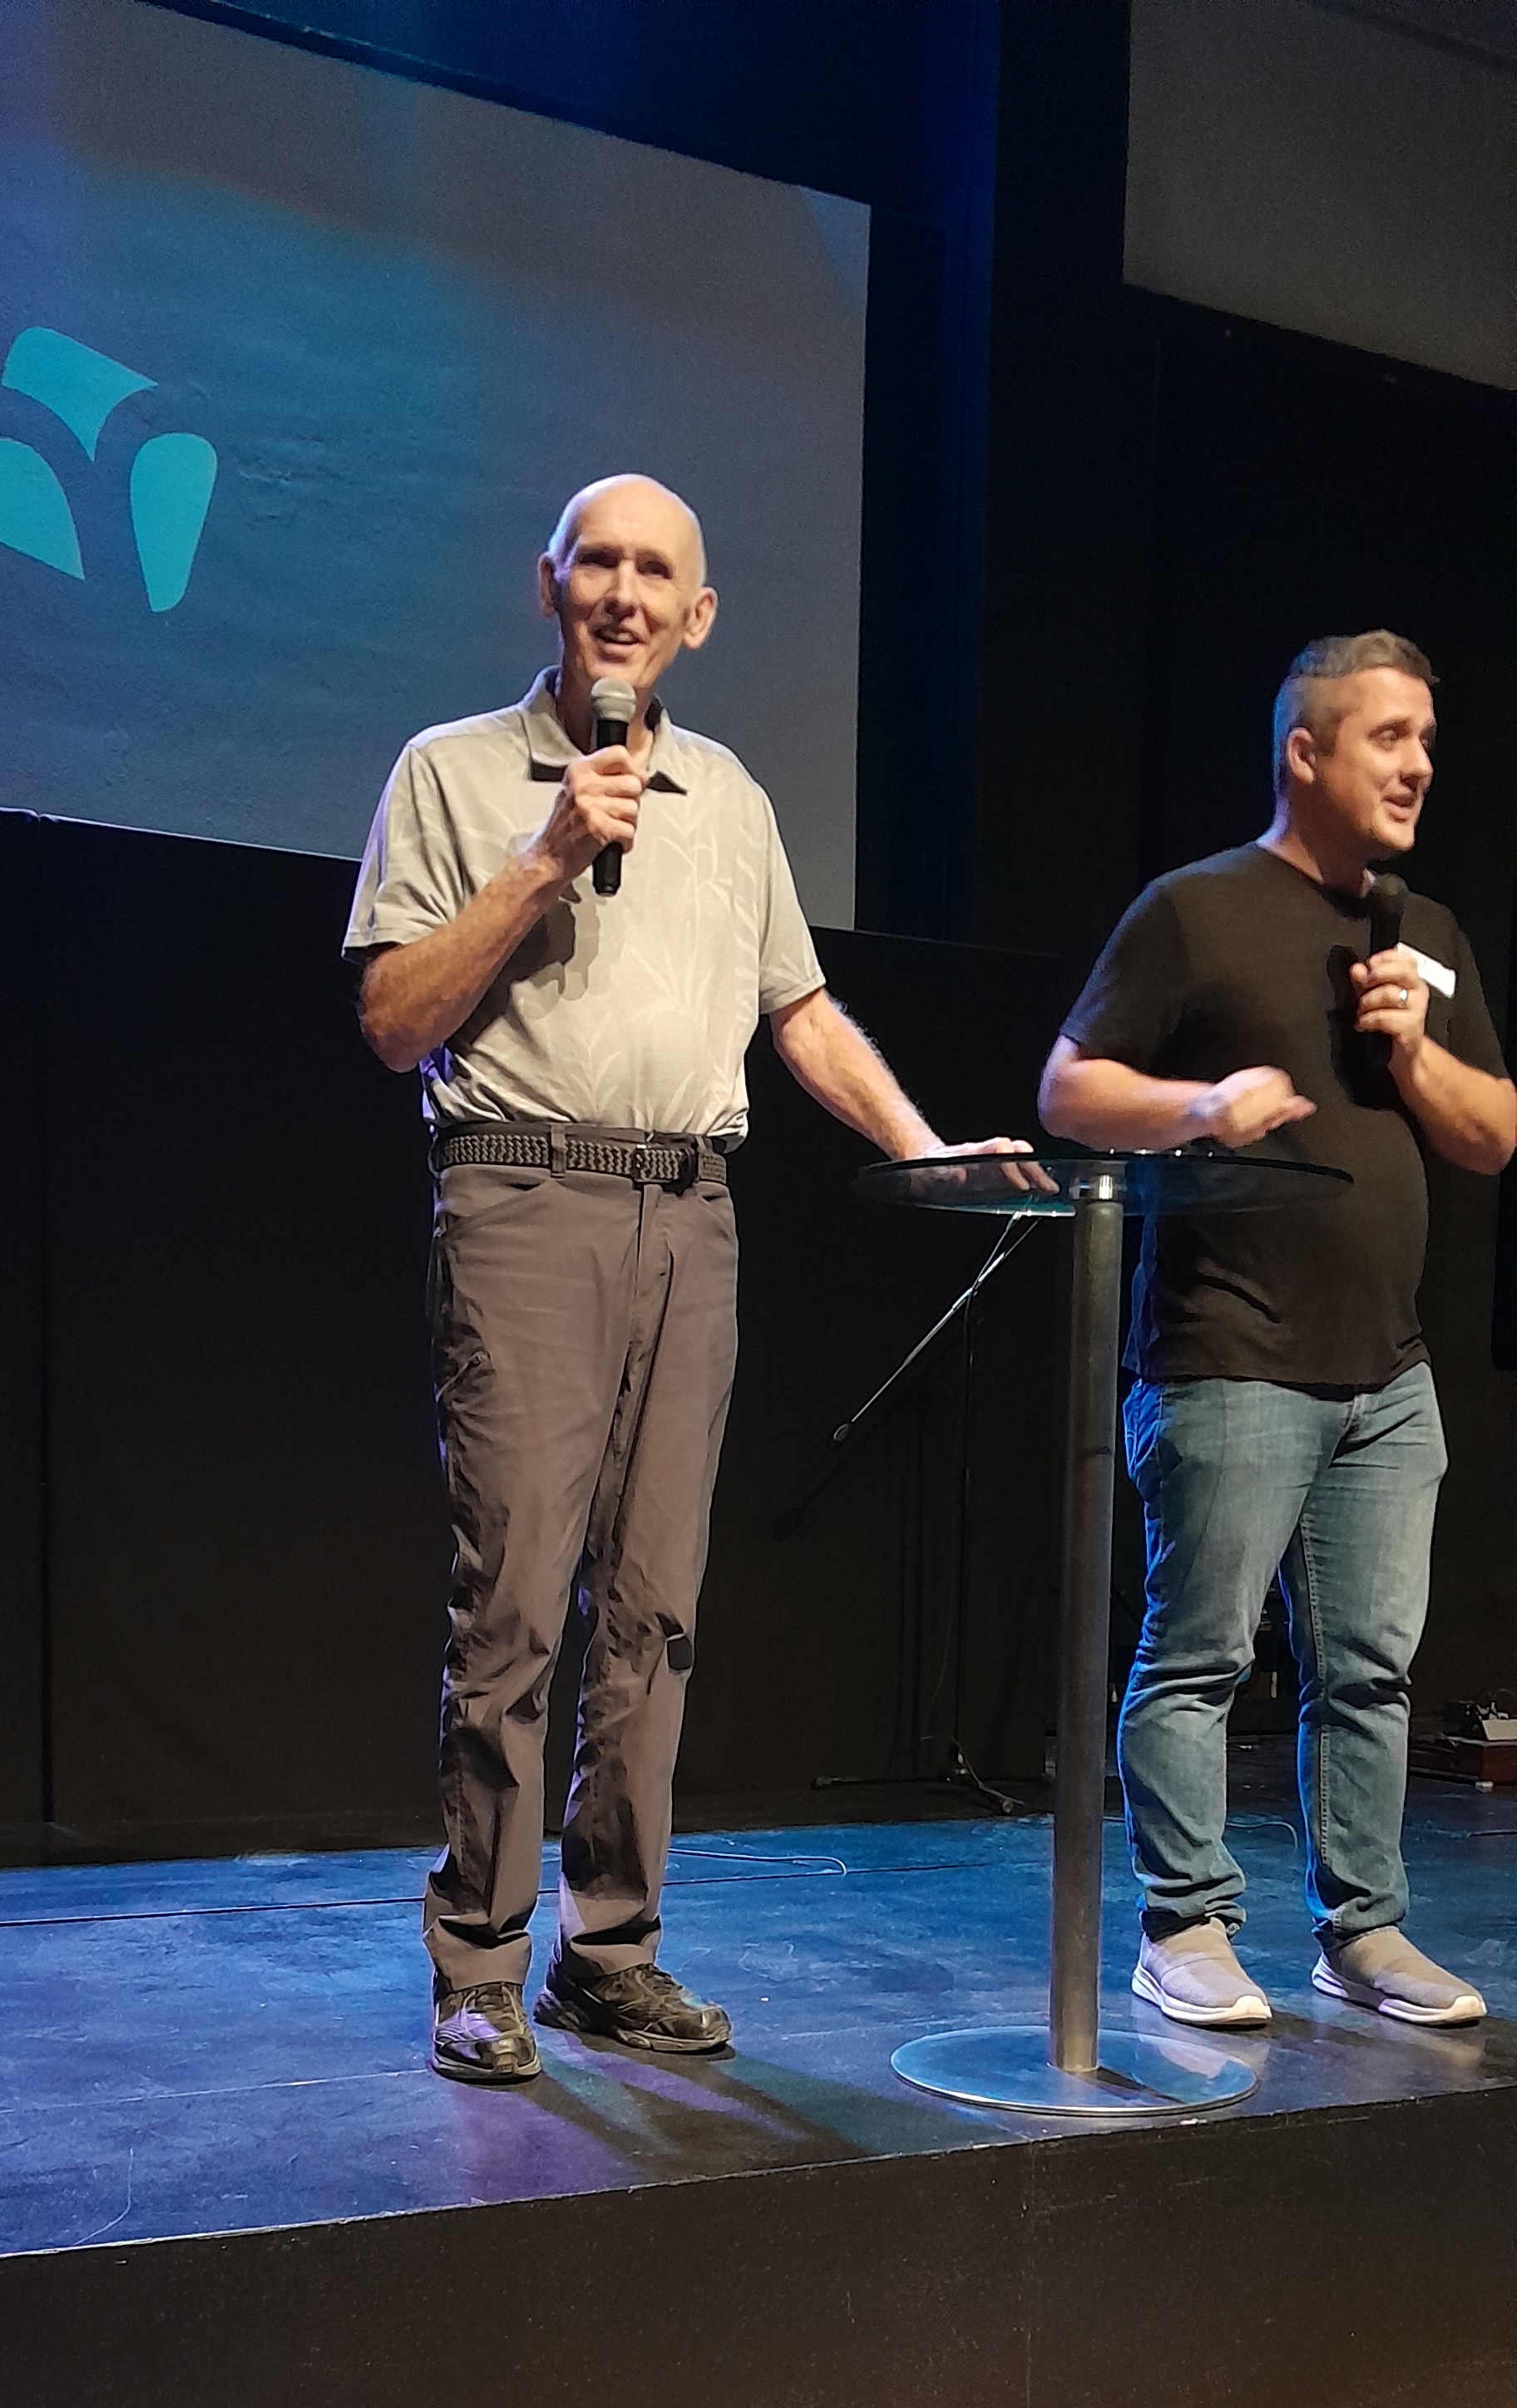
\includegraphics[scale=.5]{images/01.jpg}}
		\captionsetup{font=normalsize}
		\captionof*{figure}{I am preaching again at La Fuente in Mexico, accompanied by a translator, 2024.}
\end{minipage}\\

\thispagestyle{plain}
%For creating an image with a caption:
\begin{minipage}{\linewidth}
		\makebox[\linewidth]{%
		\centering
		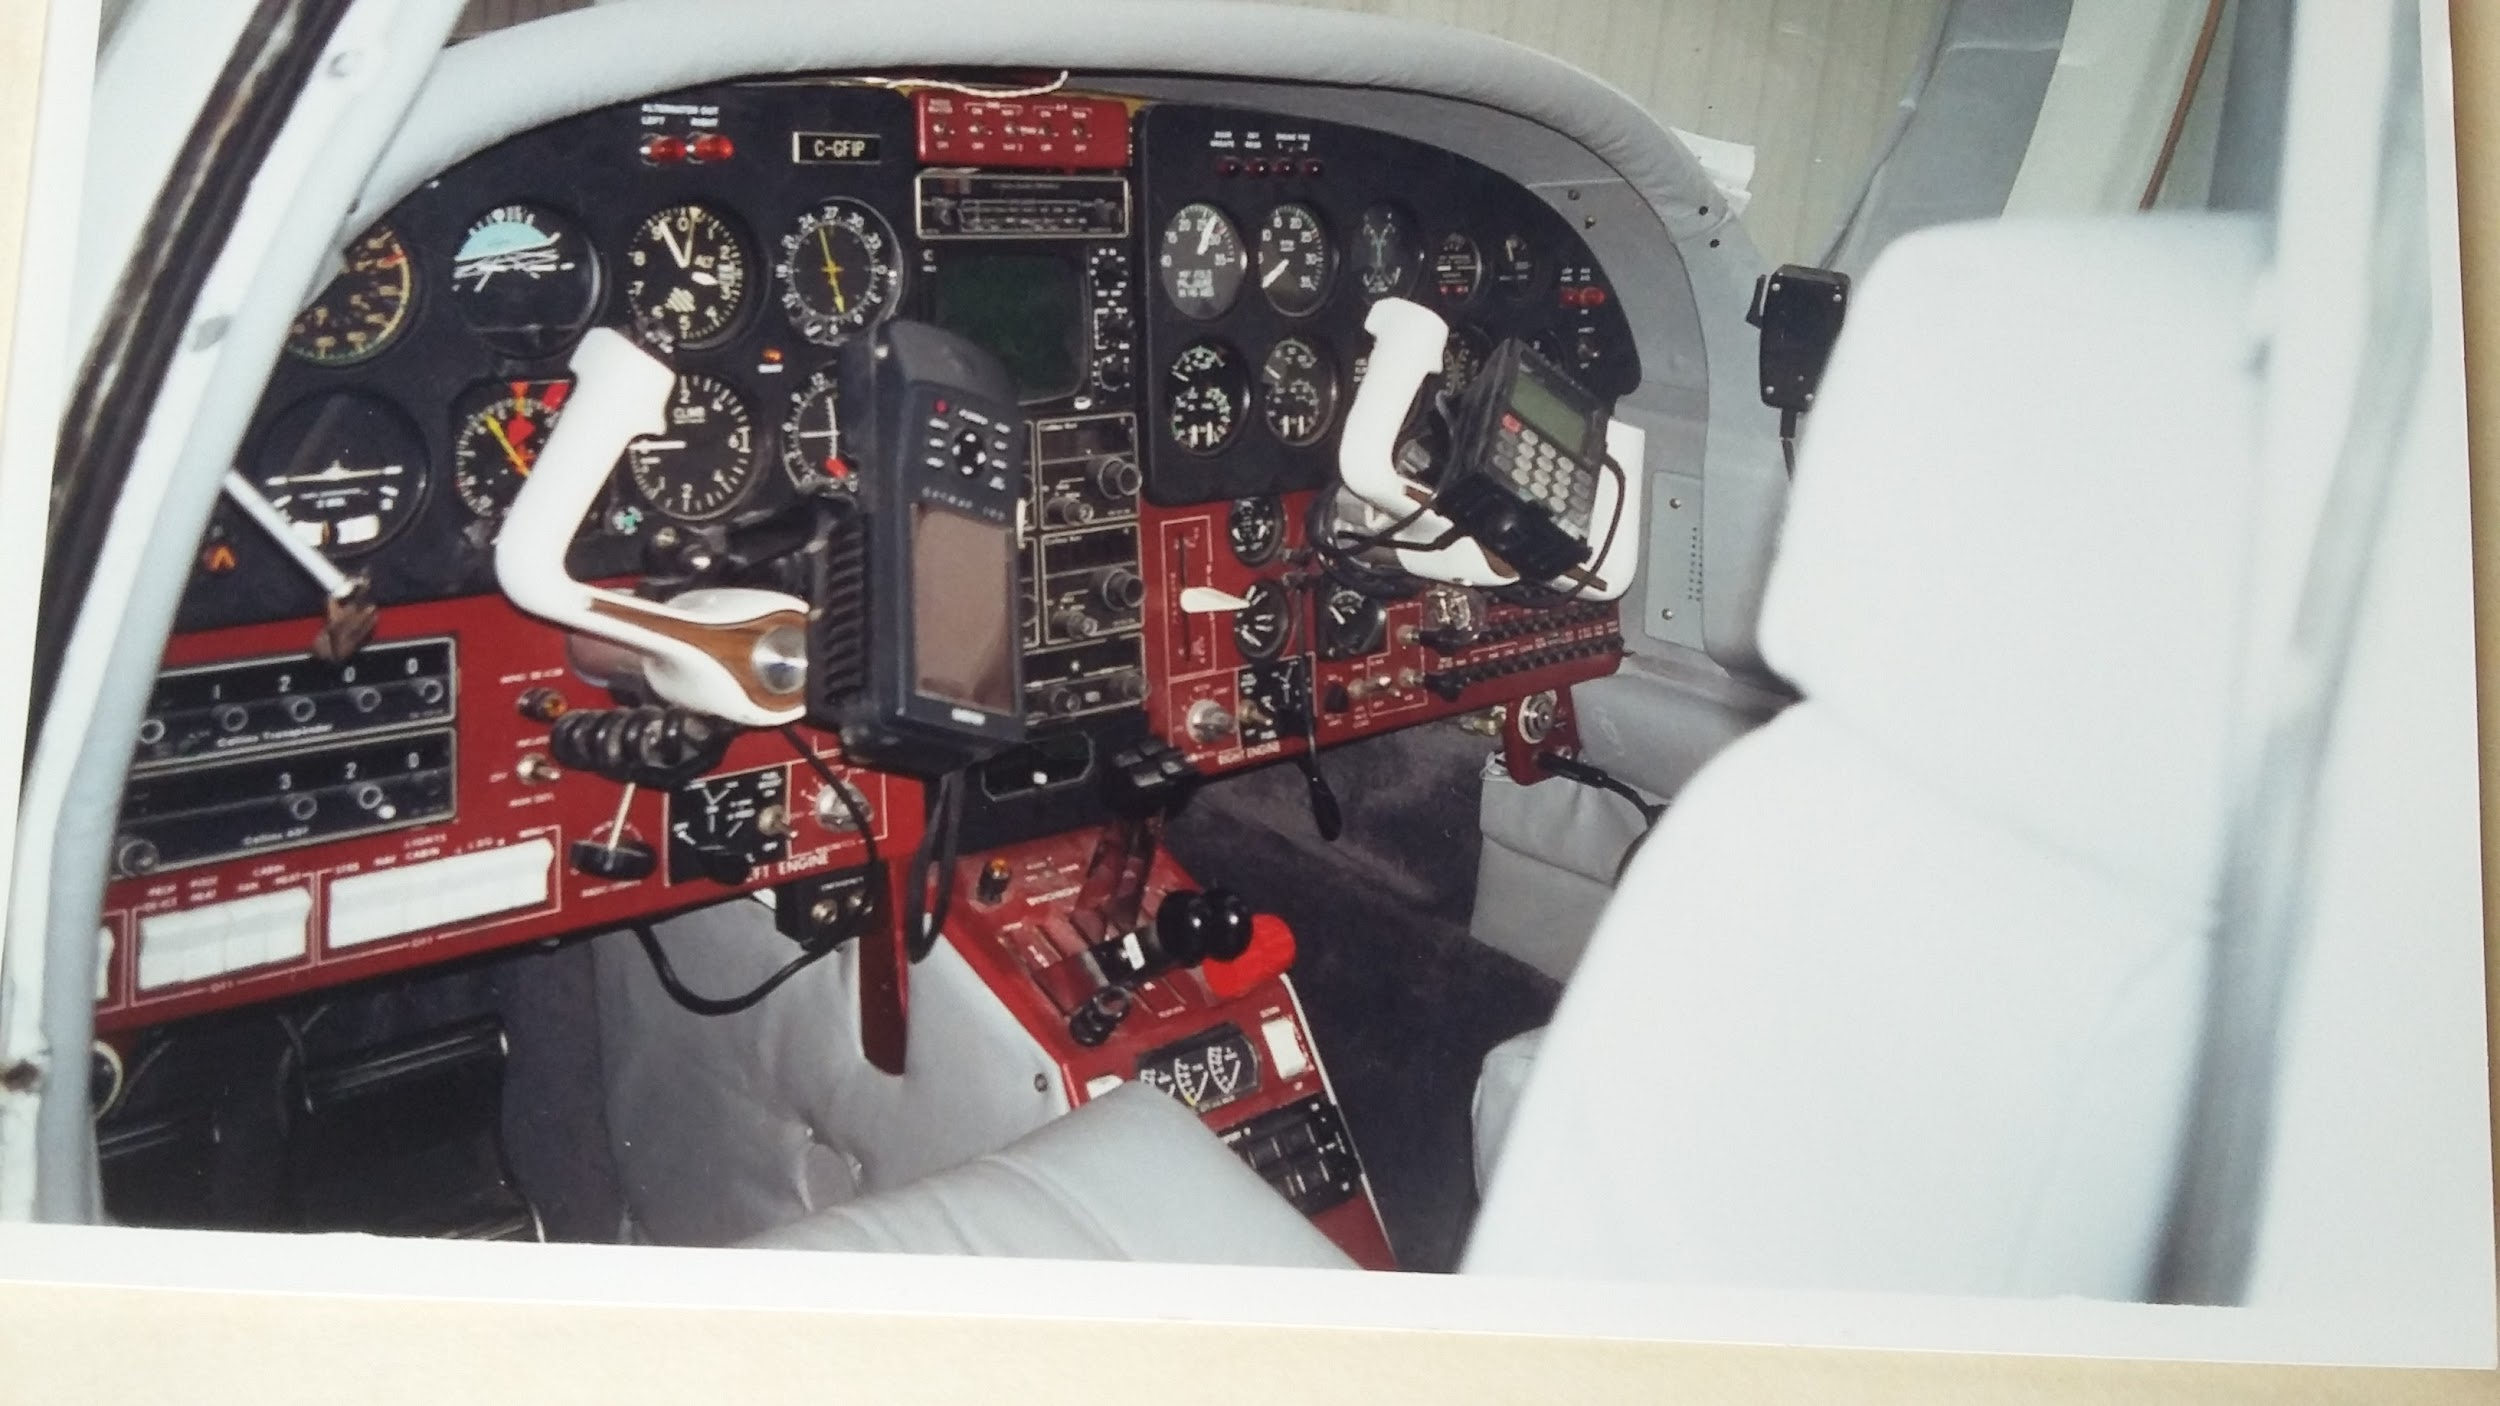
\includegraphics[scale=.1]{images/02.jpg}}
		\captionsetup{font=normalsize}
		\captionof*{figure}{Este es el último avión de cinco que tenía.  Es el Piper Aerostar con cabina presurizada de doble motor. Lo volé por más de 320,000 km, cumpliendo viajes del ministerio, aún hasta El Alto Ártico de Canadá.  }
\end{minipage}\\
\clearpage

\thispagestyle{plain}
\begin{minipage}{\linewidth}
		\makebox[\linewidth]{%
		\centering
		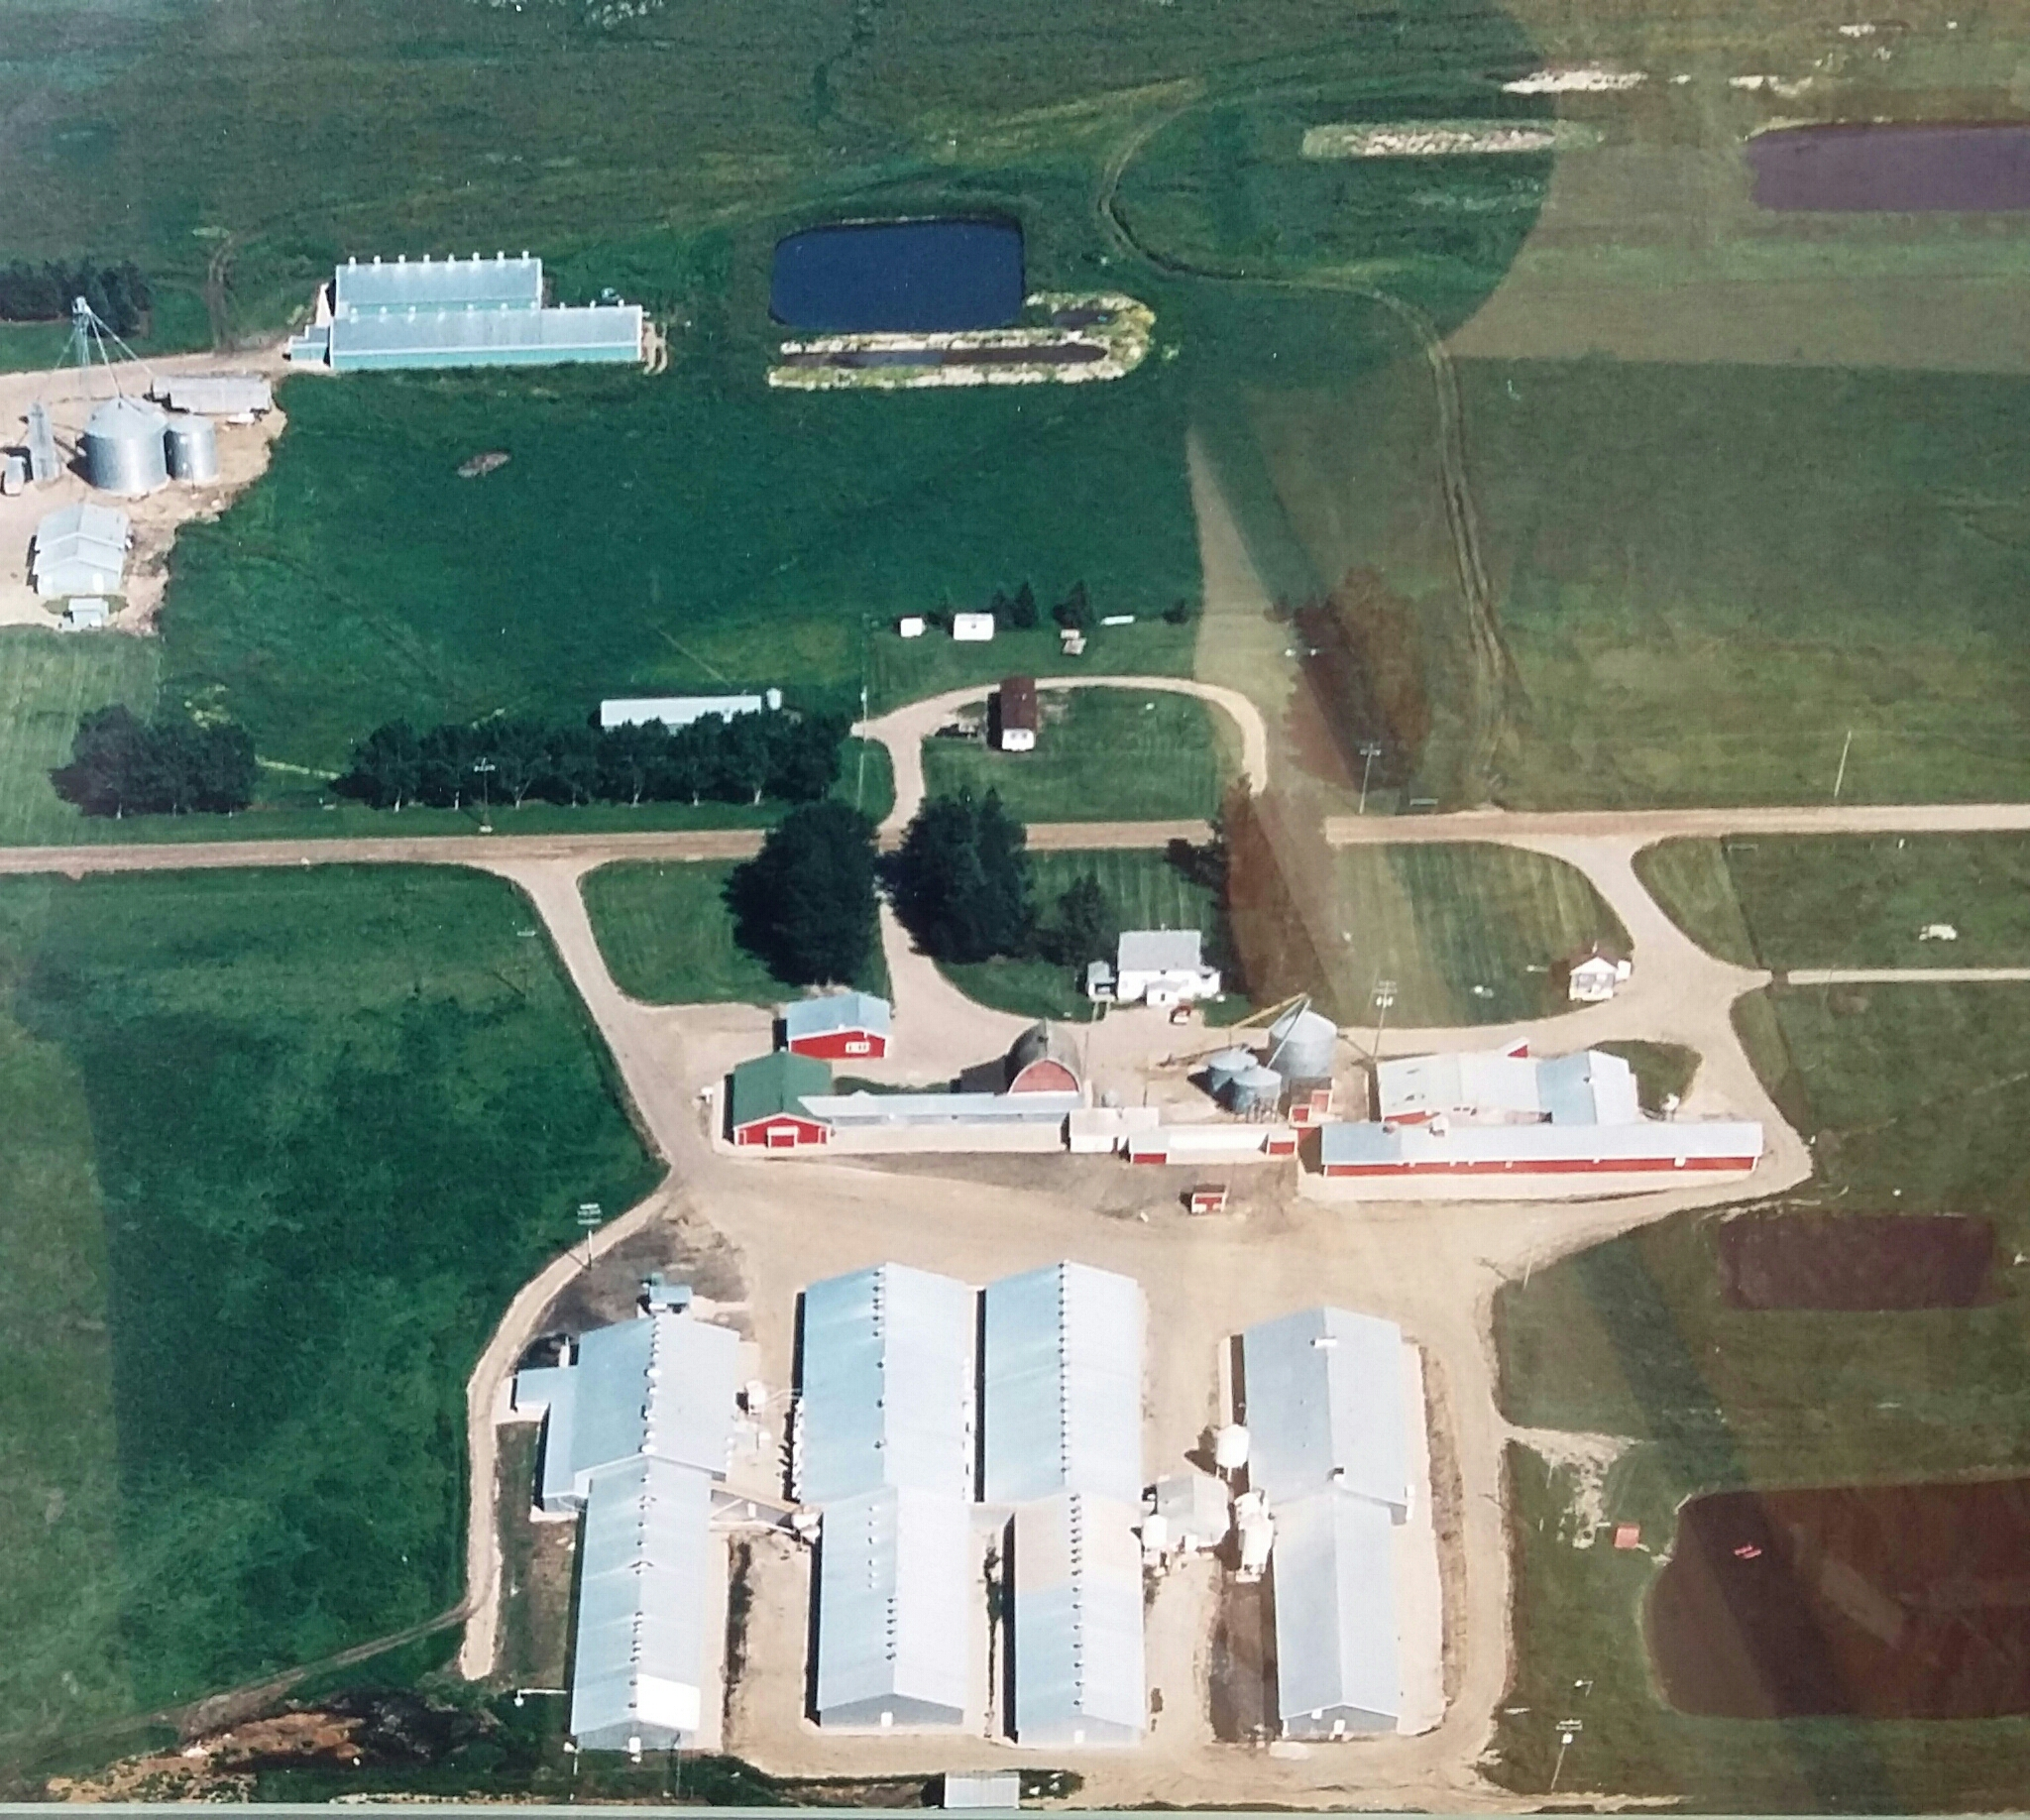
\includegraphics[scale=.1]{images/03.jpg}}
		\captionsetup{font=normalsize}
		\captionof*{figure}{La cabina de mando para el Aerostar, volando por todo tipo de clima en este asiento en todo Canadá, los Estados Unidos y El Alto Ártico.}
\end{minipage}\\
\clearpage

\thispagestyle{plain}
\begin{minipage}{\linewidth}
		\makebox[\linewidth]{%
		\centering
		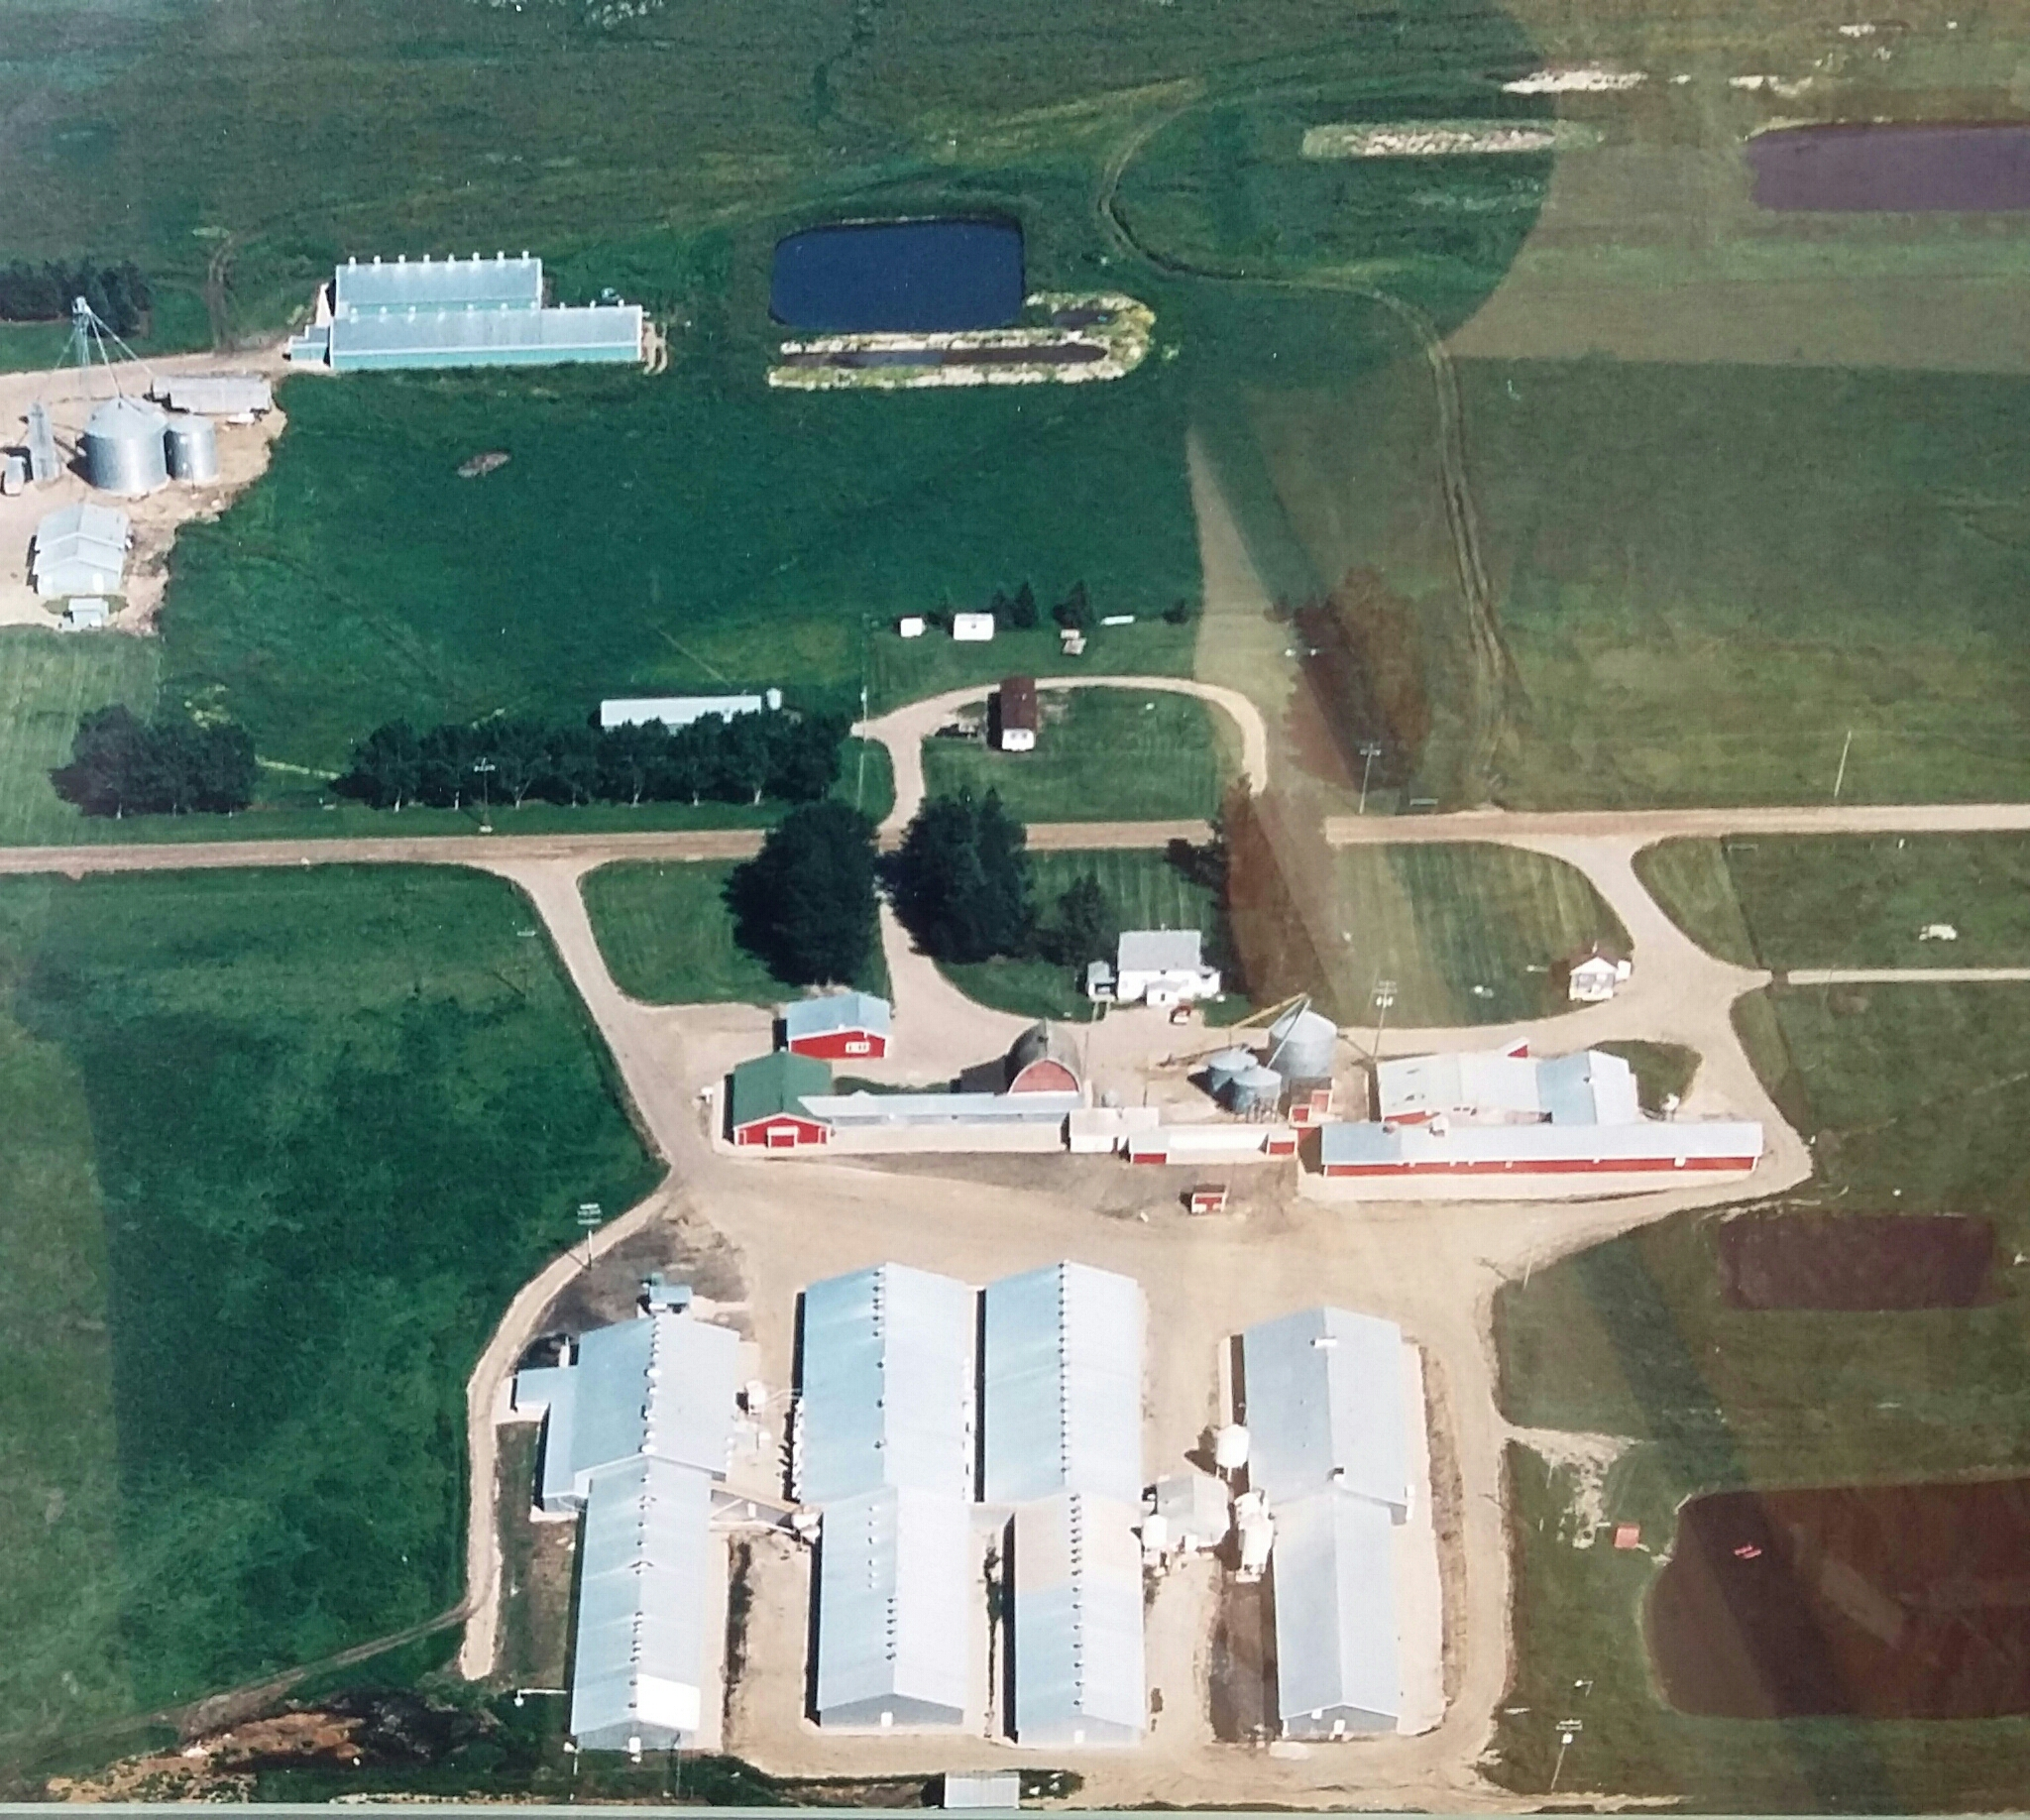
\includegraphics[scale=.15]{images/04.jpg}}
		\captionsetup{font=normalsize}
		\captionof*{figure}{Acres de Tocino, nuestra granja donde criamos más de 40,000 cerdos cada año. El granero de la derecha es donde ocurrió el incendio y donde Dios intercedió para proteger los otros edificios.}
\end{minipage}\\

\end{center}

\clearpage

\section{Algunos testimonios del Ministerio de Encuentros}

\begin{center}
\small{(printed by permission from the individuals involved)}
\end{center}
\
Es difícil poner en palabras como los encuentros de oración han cambiado mi vida. Diré que soy diferente. Sé quién soy en Cristo. Sé que Dios me ama sin ninguna duda. Sé que soy capaz de escuchar Su voz. En mi primer Encuentro, dirigido por el Pastor Dave y su primera esposa, Judy, Dios me mostró por qué yo era una persona muy controladora.  La raíz surgió de un recuerdo de mi padre utilizando sus palabras altisonantes y abusadoras hacia mi persona por traerle el cepillo equivocado. La mentira colocada en mi corazón fue, “no sirves para nada”. La verdad que Jesús habló a mi corazón ese día, fue que hay cosas que hago mal, sí, pero hago la mayoría de las cosas bien y las dos están bien. Después Dios profundizó a mi miedo de perder a seres queridos. Cada vez que me despedía de mis hijos, cuando se iban a la escuela o cuando mi marido iba a trabajar, me imaginaba su funeral. La mentira vino del incidente con mi perrito,una mascota atacada por otro perro justo delante de mí. Mi padre lo llevó al veterinario y nunca regresó porque murió allí. Entonces la mentira fue que cada vez que saliera alguien de la puerta, moriría.  La verdad es sí, las personas mueren, pero no ocurre cada vez que salgan de la puerta.  Hay muchos otros…pero he llegado al punto en el que soy capaz de reconocer las mentiras del enemigo y escuchar la verdad que Jesús tiene para mí y es libertad absoluta.\\

-Dawn, Las Vegas, Nevada, USA	

\clearpage

Estaba buscando a Dios para sanar el tejido cicatricial de mi cuello uterino. Mi ciclo menstrual no vendría por sí solo. Por un año se estaba empeorando progresivamente. También habíamos tratado de quedar embarazados. Durante un año estaba segura de que la cicatriz estaba impidiendo que ocurriera el embarazo. También había estado lidiando con células precancerosas del VIH durante muchos años. La última prueba mostró que se estaba empeorando gravemente. En octubre fui a un servicio de sanidad y me senté en la parte de atrás. Por fin, me animé de que Dave y Connie orara por mí porque esa noche sintieron una unción para levantar a las personas con cáncer. Dios los llevó a lidiar con problemas profundamente arraigados de autoestima entre otras cosas. Oraron por el tejido cicatricial, y el VIH. A la semana siguiente mi ciclo llegó por si solo.  Y nunca jamás hubo más problemas.  Un mes después me hizo una de las frecuentes pruebas de Papanicolaou. Me estaban observando diligentemente para el cáncer.  La prueba regresó completamente libre de las células del VIH.  El médico parecía un poco confundido.  Mi Dios fue tan bueno conmigo.  Y finalmente, cinco meses después quedamos embarazados de nuestro hermoso bebé.  Es un regalo precioso del amor y cuidado de Dios por nosotros. \\

- Nichole, Kalispell, MT, USA
\clearpage

Asistí a mi primer Encuentro en el 2010, a eso de un año después de ser salvo.  Fui sin expectativas; solo quería experimentar lo que era un encuentro.  Dios tenía otros planes.  El viernes por la noche, el Espíritu Santo se movía fuertemente entre el equipo de Encuentro.  Durante el tiempo de oración un miembro del grupo oró conmigo sobre el perdón para mi padre.  Sentí que la falta de perdón me dejó por primera vez y sentí amor hacia mi padre. La misma persona también sabía de un dolor mucho más profundo, algo que nunca había compartido, algo enterrado por años. Ni siquiera recordaba que había sucedido; dijo que el Espíritu Santo quería que compartiera una historia sobre cuando fui molestado sexualmente de niño. En ese momento recordé la mala experiencia.  Me pregunté, “¿Cómo conoce mi historia?”  Nunca le he contado a nadie, ¡NUNCA! Sentí como si estuviera hablando con Dios y que estuviera llegando muy dentro de mi corazón y limpiando la herida que quería sanar.  Mientras reflexionaba sobre lo que la persona del equipo compartió conmigo esa mañana, le compartí mi testimonio a mi esposa.  Oramos por eso, y supe que “ese día fui liberado de esta carga.”  Durante la primera sesión de oración del sábado por la mañana, fui a platicar con la persona del grupo de mi experiencia.  Mientras me acercaba a él, fue como si él supiera porque iba hacia él.  De nuevo, sentí como si yo estuviera con Dios.  Mientras orábamos, el Espíritu Santo me regaló una paz y me vi de niño con Jesús abrazándome y diciéndome que todo estaría bien.  Una paz sobrenatural me cubrió como nunca antes había experimentado. La carga se había ido para siempre. Ese día Dios me dio la fuerza para compartir mi testimonio sobre esta experiencia y sobre mi salvación con cualquiera que el Espíritu me llevaba a compartir. Siento que fue la plataforma de lanzamiento de un ministerio que nunca supe que era posible. Desde ese fin de semana he estado en el Ministerio de Hombres ayudando a otros a liberarse de sus cargas. En el otoño de 2016 ayudé a iniciar un grupo de Encuentros de Hombres donde otros pueden reunirse y experimentar este ministerio semanalmente, el que puede transformar vidas. Alabo a Dios por ponerme hombres como David Allan en mi vida y por su ministerio y pasión por ver al pueblo de Dios liberado. ¡Amén!. \\

- Un hombre anónimo, Kalispell, Mt
\clearpage

Fui muy bendecida al ser parte de este ministerio con Dave Allan, de ambas maneras, participante y parte del equipo. El primer fin de semana que participé en el Encuentro, descubrí que sería un gran mercado para mí. Intercambié mis penas por sanidad y entendimiento.  El aceite de Gilead (yo lo conozco como ungüento, pero para mí era como aceite) fue derramado sobre mi corazón y fue restaurado. Yo no sabía que desconfiaba de Dios, pero, ¡sí! El viernes por la noche, no pude clavar mis pecados sobre la cruz.  No podía confiar en Dios; si Él pudo llevarse a mi hermano de nuestra familia, ¿cómo podría yo confiar que Él perdonaría mis pecados? Siendo muy honesta con Dios, y Él siendo honesto conmigo, expusimos las mentiras donde Satanás me tenía envuelta por los últimos 23 años.  Pude llorar sinceramente la muerte de mi hermano. Vi a un ángel derramar aceite sobre mi corazón y físicamente lo sentí a través de mi cuerpo. Ahora cuando escucho hablar sobre la muerte ya no siento un hueco profundo, pero sí, hay un corazón completo.  Intercambié mi vergüenza por el amor de Dios, y Su aceptación a través de recuerdos revelados. Pude darme cuenta donde se encontraba Jesús durante los momentos difíciles. Trasladé el hecho de que Jesús me ama de mi cabeza a mi corazón. Yo era una persona a quien le importaban extremadamente mis habilidades. Tenía que hacerlo todo bien y controlar todo porque tenía mucho miedo de fallarle a la gente…pero con cada recuerdo que yo tenía, Dave me preguntaba ¿dónde se encuentra Jesús? ¿Mis expectativas? yo esperaba que Él estuviera lejos, con otras personas, pero siempre estaba a mi lado.  Vi una multitud de ángeles en el Cielo y Jesús y yo parados frente a ellos.  Mientras Jesús me presentaba, ellos me aplaudían.  Pude sentir a Jesús diciendo “esta es mi hija en quien estoy muy contento”.  Isaías 50:7 dice, “Porque el Señor DIOS me ayudará, por tanto, no me avergoncé, por eso puse mi rostro como un pedernal, y sé que no seré avergonzado.”  Al principio tenía miedo de ir a los encuentros; tenía miedo de que se mostrara toda mi vergüenza y la gente viera que yo era un fraude; pero Dios no me avergonzó, me levantó a un lugar de sanidad.  Ahora yo sé que puedo confiar en Dios y ¡Él nunca me avergonzará!  Ese fin de semana fue el comienzo de tener una vida sin las mentiras que me habían obligado creer. Intercambié esas mentiras por la verdad y ¡la Verdad me ha liberado totalmente!  Como participante y parte del equipo me sentía muy bendecida de ver a tantas personas liberarse de su esclavitud. Me sorprendió la cantidad de veces que Jesús apareció y en la manera que cada persona necesitaba.  Los encontró en sus lugares más oscuros y les mostró Su verdad. El poder que sentí cuando hacía este ministerio era inexplicable. Dios aparecía y su presencia era palpable. Una vez estaba orando por una mujer y sentí que los demonios comenzaron a atacarme. Sentí una pesadez increíble y me apretó como una serpiente alrededor de la garganta. Otro participante del equipo llamó a Dave y él vino y comenzó a orar por mí, específicamente hablando con el espíritu de la muerte. Recuerdo estar acostada en el suelo sintiendo como si estuviera siendo exprimida por una enorme serpiente, sintiendo que todos mis miedos se volvían tan grandes que me estaban dominando. Mientras él oraba, llamó al espíritu y le ordenó que se fuera; tomó autoridad sobre los demonios y fueron atados y echados. Físicamente, sentí que los demonios se iban y la paz que me llenó, fue verdaderamente una paz que superó a todo entendimiento (Fil 4:7) Esta experiencia fue ambos, aterradora y reconfortante. Fue una gran confirmación de que no luchamos contra la carne y la sangre sino contra los gobernantes, contra las autoridades, contra los poderes cósmicos, sobre esta oscuridad actual y contra las fuerzas espirituales del mal en los lugares celestiales (Efesios 6:12). He sentido físicamente esos poderes y he sentido el poder que el nombre de Jesús tiene sobre ellos. Es un consuelo saber que nada es más grande o más fuerte que ese precioso nombre. A menudo en nuestro mundo occidental no reconocemos el lado espiritual de los vivos. Pero esto me abrió los ojos a la realidad. Aprendí que los demonios son reales, pero también aprendí a través de esa experiencia que Jesús es más poderoso. Y está listo para salvar y proteger; todo lo que tenemos que hacer es pedirle. \\

- Shelley, Alberta, Canada
\clearpage

\addtocontents{toc}{\protect\addvspace{10pt}}
\addtocontents{toc}{\textbf{APPENDIX}}

\end{document}